\documentclass[graybox,envcountchap,sectrefs]{svmono}

\usepackage{mathptmx}
\usepackage{helvet}
\usepackage{courier}

\usepackage{type1cm}         
\usepackage{exercise}
\usepackage{makeidx}         % allows index generation
\usepackage{graphicx}        % standard LaTeX graphics tool
                             % when including figure files
\usepackage{multicol}        % used for the two-column index
\usepackage[bottom]{footmisc}% places footnotes at page bottom
\usepackage[usenames,dvipsnames,x11names]{xcolor}
 \usepackage{listings}
 \usepackage{epic}
 \usepackage{eepic}
 \usepackage{a4wide}
 \usepackage{color}
 \usepackage{amsmath}
 \usepackage{amssymb}
 \usepackage[T1]{fontenc}
 \usepackage{cite} % [2,3,4] --> [2--4]
 \usepackage{shadow}
 \usepackage{hyperref}
 \usepackage{bezier}
 \usepackage{pstricks}
% \usepackage{refcheck}
\setcounter{tocdepth}{2}

\usepackage{textcomp,type1ec,pdfpages}
\usepackage{bera}



\makeindex             % used for the subject index
                       % please use the style svind.ist with
                       % your makeindex program

%%%%%%%%%%%%%%%%%%%%%%%%%%%%%%%%%%%%%%%%%%%%%%%%%%%%%%%%%%%%%%%%%%%%%

\begin{document}

\author{Morten Hjorth-Jensen, Maria Paola Lombardo, and Ubirajara Van Kolck, Editors}
\title{An advanced course in computational nuclear physics}
 \subtitle{Bridging the scales from quarks to neutron stars}
\date{Fall 2015}
\maketitle

\frontmatter%%%%%%%%%%%%%%%%%%%%%%%%%%%%%%%%%%%%%%%%%%%%%%%%%%%%%%

%\include{dedic}
%\include{foreword}
\preface
This graduate-level text collects and synthesizes ten series of
lectures on the nuclear quantum many-body problem - starting from our
present understanding of the underlying forces with a presentation of
recent advances within the field of lattice quantum chromodynamics,
via effective field theories to central many-body methods like Monte
Carlo methods, coupled cluster theories, the similarity renormalization group approach, Green's function methods 
and large-scale
diagonalization approaches.

In particular algorithmic and computational advances show promise for
breakthroughs in predictive power including proper error estimates, a
better understanding of the underlying effective degrees of freedom
and of the respective forces at play.

Enabled by recent advances in theoretical, experimental and numerical
techniques, the modern and state-of-the art applications considered in
this volume span the entire range from our smallest components, quarks
and gluons as the mediators of the strong force to the computation of
the equation of state for neutron star matter.

 

The present lectures provide a proper exposition of the underlying
theoretical and algorithmic approaches as well as strong ties to the
numerical implementation of the exposed methods. Several of the
lectures provide links to actual numerical software and benchmark
calculations, allowing eventual readers, based upon the available
material, to develop their own programs for tackling challenging
nuclear many-body problems.


\include{acknow}

\tableofcontents

%\include{acronym}


\mainmatter%%%%%%%%%%%%%%%%%%%%%%%%%%%%%%%%%%%%%%%%%%%%%%%%%%%%%%%
\include{introduction}
\title{Quantum chromodynamics, an introduction}\label{chap:qcd}
\author{Thomas Schaefer}
\institute{Thomas Schaefer \at North Carolina State University, \email{name@email.address}}
\maketitle
\abstract{Each chapter should be preceded by an abstract (10--15 lines long) that summarizes the content. The abstract will appear \textit{online} at \url{www.SpringerLink.com} and be available with unrestricted access. This allows unregistered users to read the abstract as a teaser for the complete chapter. As a general rule the abstracts will not appear in the printed version of your book unless it is the style of your particular book or that of the series to which your book belongs.\newline\indent
Please use the 'starred' version of the new Springer \texttt{abstract} command for typesetting the text of the online abstracts (cf. source file of this chapter template \texttt{abstract}) and include them with the source files of your manuscript. Use the plain \texttt{abstract} command if the abstract is also to appear in the printed version of the book.}

\section{QCD and Symmetries}
\section{QCD at high Temperature}
\section{QCD at high Temperature: Experiment}
\section{QCD at Finite Density}
\section{Non-equilibrium QCD}



\begin{acknowledgement}
If you want to include acknowledgments of assistance and the like at the end of an individual chapter please use the \verb|acknowledgement| environment -- it will automatically render Springer's preferred layout.
\end{acknowledgement}
%
\section*{Appendix}
\addcontentsline{toc}{section}{Appendix}
%
%
When placed at the end of a chapter or contribution (as opposed to at the end of the book), the numbering of tables, figures, and equations in the appendix section continues on from that in the main text. Hence please \textit{do not} use the \verb|appendix| command when writing an appendix at the end of your chapter or contribution. If there is only one the appendix is designated ``Appendix'', or ``Appendix 1'', or ``Appendix 2'', etc. if there is more than one.

\biblstarthook{References may be \textit{cited} in the text either by number (preferred) or by author/year.\footnote{Make sure that all references from the list are cited in the text. Those not cited should be moved to a separate \textit{Further Reading} section or chapter.} The reference list should ideally be \textit{sorted} in alphabetical order -- even if reference numbers are used for the their citation in the text. If there are several works by the same author, the following order should be used: 
\begin{enumerate}
\item all works by the author alone, ordered chronologically by year of publication
\item all works by the author with a coauthor, ordered alphabetically by coauthor
\item all works by the author with several coauthors, ordered chronologically by year of publication.
\end{enumerate}
The \textit{styling} of references\footnote{Always use the standard abbreviation of a journal's name according to the ISSN \textit{List of Title Word Abbreviations}, see \url{http://www.issn.org/en/node/344}} depends on the subject of your book:
\begin{itemize}
\item The \textit{two} recommended styles for references in books on \textit{mathematical, physical, statistical and computer sciences} are depicted in ~\cite{science-contrib, science-online, science-mono, science-journal, science-DOI} and ~\cite{phys-online, phys-mono, phys-journal, phys-DOI, phys-contrib}.
\item Examples of the most commonly used reference style in books on \textit{Psychology, Social Sciences} are~\cite{psysoc-mono, psysoc-online,psysoc-journal, psysoc-contrib, psysoc-DOI}.
\item Examples for references in books on \textit{Humanities, Linguistics, Philosophy} are~\cite{humlinphil-journal, humlinphil-contrib, humlinphil-mono, humlinphil-online, humlinphil-DOI}.
\item Examples of the basic Springer style used in publications on a wide range of subjects such as \textit{Computer Science, Economics, Engineering, Geosciences, Life Sciences, Medicine, Biomedicine} are ~\cite{basic-contrib, basic-online, basic-journal, basic-DOI, basic-mono}. 
\end{itemize}
}

\begin{thebibliography}{99.}%

\end{thebibliography}

\title{Quantum Chromodynamics}
\author{Thomas Sch\"afer}
\institute{Thomas Sch\"afer \at Department of Physics, 
North Carolina State University, Raleigh, NC 27695,  USA, 
\email{tmschaef@ncsu.edu}}

\maketitle
\abstract{We present a brief introduction to QCD, the QCD phase
diagram, and non-equilibrium phenomena in QCD. We emphasize
aspects of the theory that can be addressed using computational
methods, in particular euclidean path integral Monte Carlo, 
fluid dynamics, kinetic theory, classical field theory and 
holographic duality.}



%%%%%%%%%%%%%%%%%%%%%%%%%%%%%%%%%%%%%%%%%%%%%%%%%%%%%%%%%%%%%%%%%%%%%%%%%%%
\section{Introduction}
%%%%%%%%%%%%%%%%%%%%%%%%%%%%%%%%%%%%%%%%%%%%%%%%%%%%%%%%%%%%%%%%%%%%%%%%%%%

 The goal of this chapter is to provide a brief summary of Quantum 
Chromodynamics (QCD) and the QCD phase diagram, and to give an introduction 
to computational methods that are being used to study different aspects of 
QCD. Quantum Chromodynamics is a remarkable theory in many respects. QCD 
is an almost parameter free theory. Indeed, in the context of nuclear 
physics QCD is completely characterized by the masses of the up, down,
and strange quark, and a reasonable caricature of nuclear physics emerges
in the even simpler case in which the up and down quark are taken to
be massless, and the strange quark is infinitely heavy. QCD nevertheless
accounts for the incredible richness of the phase diagram of strongly 
interacting matter. QCD describes finite nuclei, normal and superfluid 
states of nuclear matter, color superconductors, hadronic gases, quark 
gluon plasma, and many other states. This rich variety of states is
reflected in the large number of computational methods that have been 
brought to bear on problems in QCD. This includes a large number 
of methods for the structure and excitations of finite Fermi systems, 
quantum Monte Carlo methods, and a variety of tools for equilibrium
and non-equilibrium statistical mechanics. 

 The bulk of this book is devoted to the study of few and many nucleon
systems. Summarizing everything else in one brief chapter is obviously
out of the question, both because of limitations of space and because
of my limited expertise. I will therefore be very selective, and focus 
on a number of very simple yet powerful ideas. This reflects, in part, 
my background, which is not primarily in computational physics. It 
also reflects my conviction that progress in computational physics is 
unfortunately often reflected in increasingly complicated codes that 
obscure the simplicity of the underlying methods. 

%%%%%%%%%%%%%%%%%%%%%%%%%%%%%%%%%%%%%%%%%%%%%%%%%%%%%%%%%%%%%%%%%%%%%%%%%%%
\section{Path integrals and the Metropolis algorithm}
\label{sec_qm}
%%%%%%%%%%%%%%%%%%%%%%%%%%%%%%%%%%%%%%%%%%%%%%%%%%%%%%%%%%%%%%%%%%%%%%%%%%%

 Consider a simple quantum mechanical problem, the motion of a particle
in a one-dimensional potential. In order to be specific I will focus
on the double well potential $V(x)=\lambda(x^2-\eta^2)^2$, where $\eta$ 
and $\lambda$ are parameters. The Hamiltonian is
\be 
\label{H_dw}
 H = \frac{p^2}{2m}+\lambda (x^2-\eta^2)^2\, . 
\ee
Using a change of variables I can set $2m=\lambda=1$. This implies that
there is only one physical parameter in this problem, the barrier 
separation $\eta$. The regime $\eta\gg 1$ corresponds to the limit 
in which the system has two almost degenerate minima that are split
by semi-classical tunneling events. The energy eigenstates and wave 
functions are solutions of the eigenvalue problem $H|n\rangle = |n\rangle 
E_n$. Once the eigenstates are known I can compute all possible 
correlation functions 
\be 
\Pi_n(t_1,t_2,\ldots,t_n) = \langle 0 |x(t_1) x(t_2) \ldots
 x(t_n)|0\rangle \, ,
\ee
by inserting complete sets of states. An alternative to the Hamiltonian 
formulation of the problem is the Feynman path integral \cite{Feynman}. 
The path integral for the anharmonic oscillator is given by 
\be
\label{pathint}
 \langle x_1| e^{-iHt_f}|x_0\rangle = 
  \int_{x(0)=x_0}^{x(t_f)=x_1} {\cal D}x\, e^{iS}, 
  \hspace{1cm}
  S=\int_0^{t_f} dt\, \left(
   \frac{1}{4}\dot{x}^4-(x^2-\eta^2)^2 \right).
\ee
This expression contains a rapidly oscillating phase factor $e^{iS}$,
which prohibits any direct numerical attempt at computing the path 
integral. The standard approach is based on analytic continuation
to imaginary time $\tau=it$. This is also referred to as Euclidean
time, because the Minkowski interval $dx^2-dt^2$ turns into the 
Euclidean expression $dx^2+d\tau^2$. In the following I will consider 
the euclidean partition function
\be
\label{z}
 Z(T) = \int {\cal D}x\, e^{-S_E}, \hspace{1cm}
  S_E=\int_0^{\beta} d\tau\, \left(
   \frac{1}{4}\dot{x}^4+(x^2-\eta^2)^2 \right),
\ee
where $\beta=1/T$ is the inverse temperature and we assume periodic 
boundary conditions $x(0)=x(\beta)$. To see that equ.~(\ref{z})
is indeed the partition function we can use equ.~(\ref{pathint}) to 
express the path integral in terms of the eigenvalues of the Hamiltonian, 
$Z(T)=\sum_n\exp(-E_n/T)$. 
In the following I will describe numerical simulations using a discretized 
version of the euclidean action. For this purpose I discretize the euclidean 
time coordinate $\tau_j=ja,\,i=1,\ldots n$ where $a=\beta/n$ is the length 
of time interval. The discretized action is given by
\be
\label{S_disc}
 S = \sum_{i=1}^{n}\left\{ \frac{1}{4a} (x_i-x_{i-1})^2
  + a(x_i^2-\eta^2)^2 \right\},
\ee
where $x_i=x(\tau_i)$. I consider periodic boundary conditions $x_0=x_n$. 
The discretized euclidean path integral is formally equivalent to the 
partition function of a statistical system of (continuous) ``spins'' 
$x_i$ arranged on a one-dimensional lattice. This statistical system 
can be studied using standard Monte-Carlo sampling methods. In the following 
I will use the Metropolis algorithm \cite{Metropolis:1953am}. Detailed
numerical studies of the euclidean path integral can be found in 
\cite{Creutz:1980gp,Shuryak:1984xr,Shuryak:1987tr,Schafer:2004xa}.

 The Metropolis method generates an ensemble of configurations
$\{x_i\}^{(k)}$ where $i=1,\ldots, n$ labels the lattice points and $k=
1,\ldots,N_{conf}$ labels the configurations. Quantum mechanical averages 
are computed by averaging observables over many configurations, 
\be 
\langle {\cal O} \rangle = \lim_{N_{conf}\to\infty}
 \frac{1}{N_{conf}}\sum_{k=1}^{N_{conf}}
 {\cal O}^{(k)}
\ee
where ${\cal O}^{(k)}$ is the value of the classical observable
${\cal O}$ in the configuration $\{x_i\}^{(k)}$. The configurations 
are generated using Metropolis updates $\{x_i\}^{(k)}\to \{x_i\}^{(k+1)}$. 
The update consists of a sweep through the lattice during which a trial 
update $x_i^{(k+1)}= x_i^{(k)} +\delta x$ is performed for every lattice 
site. Here, $\delta x$ is a random number. The trial update is accepted 
with probability
\be
 P\left(x_i^{(k)}\to x_i^{(k+1)}\right)=
   \min\left\{\exp(-\Delta S),1\right\},
\ee 
where $\Delta S$ is the change in the action equ.~(\ref{S_disc}). 
This ensures that the configurations $\{x_i\}^{(k)}$ are distributed 
according the ``Boltzmann'' distribution $\exp(-S)$. The distribution 
of $\delta x$ is arbitrary as long as the trial update is micro-reversible, 
i.~e.~is equally likely to change $x_i^{(k)}$ to $x_i^{(k+1)}$ and back. 
The initial configuration is arbitrary. In order to study equilibration 
it is useful to compare an ordered (cold) start with $\{x_i\}^{(0)}=
\{\eta\}$ to a disordered (hot) start $\{x_i\}^{(0)}=\{r_i\}$, where 
$r_i$ is a random variable. 

 The advantage of the Metropolis algorithm is its simplicity and robustness. 
The only parameter to adjust is the distribution of $\delta x$. A simple
choice is to take $\delta x$ to be a Gaussian random number, and choose the
width of the distribution so that the average acceptance rate for the trial 
updates is around $50\%$. Fluctuations of ${\cal O}$ provide an estimate 
in the error of $\langle {\cal O}\rangle$. The uncertainty is given by 
\be 
\Delta \langle {\cal O} \rangle =
 \sqrt{\frac{\langle {\cal O}^2\rangle -\langle{\cal O}\rangle^2}
            {N_{conf}}}. 
\ee
This requires some care, because the error estimate is based on 
the assumption that the configurations are statistically independent. 
In practice this can be monitored by computing the auto-correlation 
``time'' in successive measurements ${\cal O}(\{x_i\}^{(k)})$. 

 I have written a simple fortran code that implements the Metropolis 
algorithm for euclidean path integrals \cite{Schafer:2004xa}. The 
most important part of that code is a sweep through the lattice 
with a Metropolis update on every site $\tau_j$: 

\vspace*{0.3cm} 
\begin{lstlisting}
 do j=1,n-1
            
         nhit = nhit+1  
          
         xpm = (x(j)-x(j-1))/a
         xpp = (x(j+1)-x(j))/a
         t = 1.0/4.0*(xpm**2+xpp**2)
         v = (x(j)**2-f**2)**2
         sold = a*(t+v)

         xnew = x(j) + delx*(2.0*ran2(iseed)-1.0)
             
         xpm = (xnew-x(j-1))/a
         xpp = (x(j+1)-xnew)/a
         t = 1.0/4.0*(xpm**2+xpp**2)
         v = (xnew**2-f**2)**2
         snew = a*(t+v)
         dels = snew-sold           
                       
         p  = ran2(iseed)          
         if (exp(-dels) .gt. p) then
            x(j) = xnew
            nacc = nacc + 1
         endif
            
enddo
\end{lstlisting}

\vspace*{0.3cm} 
 Here, {\tt sold} is the local action corresponding to the initial
value of ${\tt x(j)}$, and {\tt snew} is the action after the trial
update. The trial update is accepted if {\tt exp(-dels)} is greater
that the random variable ${\tt p}$. The function {\tt ran2()} generates 
a random number between 0 and 1, and {\tt nacc/nhit} measures the 
acceptance rate. A typical path is shown in Fig.~\ref{fig_path}. An 
important feature of the paths in the double well potential is the 
presence of tunneling events. Indeed, in the semi-classical regime 
$\eta\gg 1$, a typical path can be understood as Gaussian fluctuations 
superimposed on a series of tunneling events (instantons). 

%%%%%%%%%%%%%%%%%%%%%%%%%%%%%%%%%%%%%%%%%%%%%%%%%%%%%%%%%%%%%%%%%%%%%%%%%%%
\begin{figure}[t]
\begin{center}
\includegraphics[width=9cm]{Chapter2-figures/config1.pdf}  
\end{center}  
\caption{\label{fig_path}
Typical euclidean path obtained in a Monte Carlo simulation
of the discretized euclidean action of the double well 
potential for $\eta=1.4$. The lattice spacing in the 
euclidean time direction is $a=0.05$ and the total number 
of lattice points is $N_\tau=800$. The green curve shows 
the corresponding smooth path obtained by running 100 
cooling sweeps on the original path. }
\end{figure}
%%%%%%%%%%%%%%%%%%%%%%%%%%%%%%%%%%%%%%%%%%%%%%%%%%%%%%%%%%%%%%%%%%%%%%%%%%%

 The path integral method does not provide direct access to the eigenvalues
of the Hamiltonian, but it can be used to compute imaginary time correlation
functions
\be
\label{qm_cor}
 \Pi_n^E(\tau_1,\ldots,\tau_n)=\langle x(\tau_1)\ldots x(\tau_n)\rangle.
\ee
Note that the average is carried out with respect to the partition 
function in equ.~(\ref{z}). In the limit $\beta\to\infty$ this 
corresponds to the ground state expectation value. A very important 
observable is the two-point function $\Pi^E(\tau)\equiv \Pi^E_2(0,\tau)$. 
The euclidean correlation functions is related to the eigenstates of 
the Hamiltonian via a spectral representations. This representation 
is obtained by inserting a complete set of states into 
equ.~(\ref{qm_cor}). The result is
\be 
\label{spec}
\Pi^E(\tau)= \sum_n |\langle 0|x|n\rangle|^2 
 \exp(-(E_n-E_0)\tau),
\ee
where $E_n$ is the energy of the state $|n\rangle$. This can be written as
\be
\Pi^E(\tau)= \int dE\, \rho(E) \exp(-(E-E_0)\tau),
\ee
where $\rho(E)$ is the spectral function. In the case of the double well
potential there are only bound states and the spectral function is a sum 
of delta-functions. Equ.~(\ref{spec}) shows that the euclidean correlation 
function is easy to construct once the energy eigenvalues and eigenfunctions 
are known. The inverse problem is well defined in principle, but numerically 
much more difficult. The excitation energy of the first excited state 
$\Delta E_1 = E_1-E_0$ is easy to extract from the exponential decay of the 
two-point functions, but higher states are more difficult to compute. A 
technique for determining the spectral function from 
euclidean correlation functions is the maximum entropy image reconstruction 
method, see \cite{Jarrell:1996rrw,Asakawa:2000tr}.

 The calculation of correlation functions in a Monte Carlo simulation
is very straightforward. All I need to do is multiply the values of 
$x(\tau_i)$ for a given path, and then average over all paths:
 
\vspace*{0.3cm} 
\begin{lstlisting}
do ic=1,nc
            
      ncor = ncor + 1 
      ip0 = int( (n-np)*ran2(iseed) ) 
      x0  = x(ip0) 
            
      do ip=1,np
         x1 = x(ip0+ip)
         xcor = x0*x1
         x2cor= xcor**2
         xcor_sum(ip)  = xcor_sum(ip)  + xcor
         xcor2_sum(ip) = xcor2_sum(ip) + xcor**2
   enddo  
enddo
\end{lstlisting}

\vspace*{0.3cm} 
 The advantages of this method are that it is extremely robust, that it 
requires no knowledge (or preconceived notion) of what the wave function 
looks like, and that it can explore a very complicated configuration space.
On the other hand, in the case of one-dimensional quantum mechanics, the 
Metropolis method is very inefficient. Using direct diagonalization in a 
finite basis it is not difficult to compute the energies of the first 
several states in the potential in equ.~(\ref{H_dw}) with very high accuracy, 
$\Delta E/E_0 \sim O(10^{-6})$ or better. On the other hand, using the 
Monte Carlo method, it is quite difficult to achieve an accuracy of 
$O(10^{-2})$ for observable other than $(E_1-E_0)/E_0$. The advantage of the 
Monte Carlo method is that the computational cost scales much more 
favorably in high dimensional systems, such as quantum mechanics of 
many particles, or quantum field theory.

 The Monte Carlo method also does not directly provide the ground state
energy, or the partition function and free energy at finite temperature.
In quantum mechanics we can compute the ground state energy from the 
expectation value of the Hamiltonian $\langle H\rangle = \langle T+V
\rangle$ in the limit $\beta\to\infty$. The expectation value of the kinetic 
energy is singular as $a\to 0$, but this problem can be overcome by using
the Virial theorem
\be 
\langle H\rangle = \left\langle \frac{x}{2}V'+V \right\rangle\, . 
\ee
There is no simple analog of this method in quantum field theory. A method 
for computing the free energy which does generalize to quantum field theory
is the adiabatic switching technique. The idea is to start from a reference 
system for which the free energy is known and calculate the free energy 
difference to the real system using Monte Carlo methods. For this purpose 
I write the action as 
\be 
S_\alpha=S_0+\alpha\Delta S\, , 
\ee
where $S_0$ is the action of the reference system, $\Delta S$ is defined 
by $\Delta S=S-S_0$ where $S$ is the full action, and $\alpha$ can be viewed 
as a coupling constant. The action $S_\alpha$ interpolates between the 
physical system for $\alpha=1$ and the reference system for $\alpha=0$. 
Integrating the relation $\partial \log Z(\alpha)/(\partial\alpha)=
-\langle \Delta S \rangle_\alpha$ I find
\be
\label{adiab}
 \log(Z(\alpha\!=\!1))=\log(Z(\alpha\!=\!0)) 
 - \int_0^1 d\alpha'\, \langle \Delta S\rangle_{\alpha'} \;\; ,
\ee
where $\langle .\rangle_\alpha$ is computed using the action $S_\alpha$. In 
the case of the anharmonic oscillator it is natural to use the harmonic 
oscillator as a reference system. In that case the reference partition
function is 
\be 
 Z(\alpha\!=\!0) = \sum_n \exp(-\beta E_n^0) 
  = \frac{\exp(-\beta\omega_0/2)}{1-\exp(-\beta\omega_0)},
\ee
where $\omega_0$ is the oscillator constant. Note that the free energy 
$F=T\log(Z)$ of the anharmonic oscillator should be independent of the 
reference frequency $\omega_0$. The integral over the coupling constant 
$\alpha$ can be calculated in a Monte Carlo simulation by slowly changing 
$\alpha$ from 0 to 1 during the simulation. Free energy calculations of 
this type play an important role in quantum chemistry, and more efficient 
methods for determining $\Delta F$ have been developed \cite{Jarzynski:1997}.


%%%%%%%%%%%%%%%%%%%%%%%%%%%%%%%%%%%%%%%%%%%%%%%%%%%%%%%%%%%%%%%%%%%%%%%%%%%
\section{Quantumchromodynamics}
\subsection{QCD at zero temperature and density}
\label{sec_qcd}
%%%%%%%%%%%%%%%%%%%%%%%%%%%%%%%%%%%%%%%%%%%%%%%%%%%%%%%%%%%%%%%%%%%%%%%%%%%

 The rich phenomenology of strong interacting matter is encoded in a 
deceptively simple Lagrangian. The fundamental fields in the Lagrangian 
are quark fields $q_{\alpha\, f}^c$ and gluon fields $A_\mu^a$. Here, $\alpha=1,
\ldots,4$ is a Dirac spinor index, $c=1,\ldots,N_c$ with $N_c=3$ is a 
color index, and $f={\it up}, {\it down},{\it strange}, {\it charm},
{\it bottom}, {\it top}$ is a flavor index. Interactions in QCD are
governed by the color degrees of freedom. The gluon field $A_\mu^a$ is 
a vector field labeled by an index $a=1,\ldots,N_c^2-1$ in the adjoint
representation. The $N_c^2-$ multiplet of gluon fields can be used to 
construct a matrix valued field $A_\mu=A_\mu^a \frac{\lambda^a}{2}$, where 
$\lambda^a$ is a set of traceless, Hermitian, $N_c\times N_c$ matrices. 
The QCD Lagrangian is
\be
\label{l_qcd}
 {\cal L } =  - \frac{1}{4} G_{\mu\nu}^a G_{\mu\nu}^a
  + \sum_f^{N_f} \bar{q}_f ( i\gamma^\mu D_\mu - m_f) q_f\, ,
\ee
where $G^a_{\mu\nu}$ is the QCD field strength tensor defined by 
\be
 G_{\mu\nu}^a = \partial_\mu A_\nu^a - \partial_\nu A_\mu^a
  + gf^{abc} A_\mu^b A_\nu^c\, ,
\ee
and $f^{abc}=4i\,{\rm Tr}([\lambda^a,\lambda^b]\lambda^c)$ are 
the $SU(N_c)$ structure constants. The action of the covariant 
derivative on the quark fields is 
\be
 i D_\mu q =  \left(
 i\partial_\mu + g A_\mu^a \frac{\lambda^a}{2}\right) q\, ,
\ee
and $m_f$ is the mass of the quarks. The terms in equ.~(\ref{l_qcd}) 
describe the interaction between quarks and gluons, as well as nonlinear 
three and four-gluon interactions. Note that, except for the number 
of flavors and their masses, the structure of the QCD Lagrangian is
completely fixed by the local $SU(N_c)$ color symmetry.

 A natural starting point for studying the phase diagram of hadronic 
matter is to consider the light flavors (up, down, and strange) as
approximately massless, and the heavy flavors (charm, bottom, top) as
infinitely massive. In this limit the QCD Lagrangian is completely
characterized by two integer valued parameters, the number of colors 
$N_c=3$ and flavors $N_f=3$, and a single dimensionless coupling 
constant $g$. Quantum fluctuations cause the coupling constant
to become scale dependent \cite{Gross:1973id,Politzer:1973fx}. At 
one-loop order the running coupling constant is
\be
\label{g_1l}
 g^2(q^2) = \frac{16\pi^2}
  {b_0\log(q^2/\Lambda_{\it QCD}^2)}\, , \hspace{1cm}
 b_0=\frac{11}{3}N_c-\frac{2}{3}N_f\, ,
\ee
where $q$ is a characteristic momentum and $N_f$ is the number of active 
flavors. The scale dependence of the coupling implies that, as a quantum 
theory, QCD is not governed by a dimensionless coupling but by a 
dimensionful scale, the QCD scale parameter $\Lambda_{\it QCD}$. This 
phenomenon is known as dimensional transmutation~\cite{Coleman:1973jx}. 

 A crucial aspect of the scale dependence of the coupling in QCD is that
the effective interaction decreases as the energy or momentum scale is 
increased. This feature of QCD is called asymptotic freedom
\cite{Gross:1973id,Politzer:1973fx}. It implies that high energy 
interactions can be analyzed using perturbative QCD. The flip side of 
asymptotic freedom is anti-screening, or confinement: The effective 
interaction between quarks increases with distance, and quarks are 
permanently confined into hadrons. The absence of colored states in 
the spectrum implies that the use of perturbation theory is subtle, 
even at high energy. Quantities that can be computed perturbatively 
either involve a sum over many hadronic states, or allow for a 
factorization of perturbative interactions and non-perturbative 
matrix elements. 

 If quarks are massless then QCD observables are dimensionless ratios
like $m_p/\Lambda_{\it QCD}$, where $m_p$ is the mass of the proton. This
implies that the QCD scale is not a parameter of the theory, but reflects
a choice of units. In the real world QCD is part of the standard model,
quarks acquire masses by electroweak symmetry breaking, and the QCD 
scale is fixed by value of the coupling constant at the weak scale. 
Experiments determine the value of the QCD fine structure constant
$\alpha_s=g^2/(4\pi)$ at the position of the $Z$ boson pole, $\alpha_s
(m_z)= 0.1184\pm 0.0007$ \cite{Nakamura:2010zzi}. The numerical value 
of $\Lambda_{QCD}$ depends on the renormalization scheme used in
computing quantum corrections to the coupling constant. Physical 
observables, as well as the value of $b_0$, are independent of this 
choice. In the modified minimal subtraction ($\overline{MS}$) scheme
the scale parameter is $\Lambda_{QCD}\simeq 200$ MeV \cite{Nakamura:2010zzi}.

%%%%%%%%%%%%%%%%%%%%%%%%%%%%%%%%%%%%%%%%%%%%%%%%%%%%%%%%%%%%%%%%%%%%%%%%%
\begin{figure}[t]
\bc\includegraphics[width=0.7 \textwidth]{Chapter2-figures/qcd_ms_high.pdf}\ec
\caption{\label{fig_qcd_phase}
Schematic phase diagram of QCD as a function of temperature $T$ and
baryon chemical potential $\mu$. The quark gluon plasma phase is 
labeled QGP, and CFL refers to the color superconducting phase 
that is predicted to occur at asymptotically large chemical potential. 
The critical endpoints of the chiral and nuclear liquid-gas phase 
transitions, are denoted by red and black points, respectively. 
The chiral pseudo-critical line associated with the crossover transition
at low temperature is shown as a dashed line.  The green arrows indicate
the regions of the phase diagram that can be studied by the experimental 
heavy ion programs at RHIC and the LHC.}
\end{figure}
%%%%%%%%%%%%%%%%%%%%%%%%%%%%%%%%%%%%%%%%%%%%%%%%%%%%%%%%%%%%%%%%%%%%%%%%%

 A schematic phase diagram of QCD is shown in Fig.~\ref{fig_qcd_phase}.
In this figure I show the phases of strongly interacting matter as a 
function of the temperature $T$ and the baryon chemical potential $\mu$. 
The chemical potential $\mu$ controls the baryon density $\rho$, defined 
as 1/3 times the number density of quarks minus the number density of 
anti-quarks. In the following I will explain that the basic structure 
of the phase diagram is determined by asymptotic freedom and the 
symmetries of QCD. For more detailed reviews see
\cite{Alford:2007xm,Adams:2012th,Braun-Munzinger:2015hba}.

 At small temperature and chemical potential the interaction between
quarks is dominated by large distances and the effective coupling is
strong. This implies that quarks and gluons are permanently confined in
color singlet hadrons, with masses of order $\Lambda_{QCD}$. The proton,
for example, has a mass of $m_p=935$ MeV. A simplistic view of the 
structure of the proton is that it is a bound state of three constituent 
quarks with effective masses $m_Q\simeq m_p/3\simeq \Lambda_{QCD}$. These
masses should be compared to the bare up and down quark masses which are 
of the order 10 MeV.

 As a consequence of strong interactions between virtual quarks and 
anti-quarks in the QCD ground state a vacuum condensate of $\bar{q}q$ 
pairs is generated, $\langle\bar{q}q\rangle\simeq-\Lambda^3_{QCD}$
\cite{GellMann:1968rz,Coleman:1980mx,tHooft:1979bh}. This vacuum 
expectation value spontaneously breaks the approximate chiral $SU(3)_L
\times SU(3)_R$ flavor symmetry of the QCD Lagrangian down to its 
diagonal subgroup, the flavor symmetry $SU(3)_V$. Spontaneous chiral 
symmetry breaking implies the existence of Goldstone bosons, massless 
modes with the quantum numbers of the generators of the broken axial 
symmetry $SU(3)_A$. The corresponding excitations in the spectrum
of QCD are the $\pi$, $K$ and $\eta$ mesons. The $SU(3)_L\times SU(3)_R$ 
symmetry is explicitly broken by quark masses, and the mass of the 
charged pion is $m_\pi=139$ MeV. This scale can be compared to the 
mass of the lightest non-Goldstone particle, the rho meson, which 
has a mass $m_\rho=770$ MeV.

 At low energy Goldstone bosons can be described in terms of 
an effective field theory in which composite $\pi$, $K$ and 
$\eta$ particles are treated as fundamental fields. The Goldstone 
boson field can be parametrized by unitary matrices 
\be
\Sigma = \exp(i\lambda^a\phi^a/f_\pi)\, , 
\ee
where $\lambda^a$ are the Gell-Mann matrices for $SU(3)$ flavor 
and $f_\pi=93$ MeV is the pion decay constant. For example, $\pi^0=\phi^3$ 
and $\pi^\pm=(\phi_1\pm i\phi_2)/2$ describe the neutral and charged pion. 
Other components of $\phi^a$ describe the neutral and charged kaons, as 
well as the eta. The eta prime, which is the $SU(3)_F$ singlet meson,
acquires a large mass because of the axial anomaly, and is not a Goldstone 
boson. The axial anomaly refers to the fact that the flavor singlet
axial current, which is conserved in massless QCD at the classical
level, is not conserved if quantum effects are taken into account. The
divergence of the axial current $A_\mu=\bar{q}\gamma_\mu\gamma_5 q$ is 
\be 
\partial_\mu A^\mu = \frac{g^2N_f}{32\pi^2} 
\epsilon^{\mu\nu\alpha\beta}
      G^a_{\mu\nu}G^a_{\alpha\beta} \, . 
\ee
The right hand side is the topological charge density, which I will
discuss in more detail in Sect.~\ref{sec_QCD_vac}.

 At low energy the effective Lagrangian for the chiral field can be 
organized as a derivative expansion in gradients of $\Sigma$. Higher 
derivative terms describe interactions that scale as either the 
momentum or the energy of the Goldstone boson. Since Goldstone bosons 
are approximately massless, the energy is of the same order of magnitude 
as the momentum. We will see that the expansion parameter is $p/(4\pi 
f_\pi)$. At leading order in $(\partial/f_\pi)$ there is only one 
possible term which is consistent with chiral symmetry, Lorentz invariance 
and the discrete symmetries $C,P,T$. This is the Lagrangian of the 
non-linear sigma model
\be
\label{l_chpt}
{\mathcal L} = \frac{f_\pi^2}{4} {\rm Tr}\left[
 \partial_\mu\Sigma\partial^\mu\Sigma^\dagger\right] 
  +\left[ B {\rm Tr}(M\Sigma^\dagger) + h.c. \right]
+ \ldots. \, , 
\ee
where the term proportional to $B$ takes into account explicit symmetry 
breaking. Here, $M={\rm diag}(m_u,m_d,m_s)$ is the quark mass matrix 
and $B$ is a low energy constant that I will fix below. 

 First, I will show that the parameter $f_\pi$ controls the pion decay 
amplitude. For this purpose I have to gauge the weak $SU(2)_L$ symmetry
of the non-linear sigma model. 
As usual, this is achieved by promoting the derivative to a gauge covariant 
operator $\nabla_\mu\Sigma = \partial_\mu\Sigma+ig_w W_\mu\Sigma$ where 
$W_\mu$ is the charged weak gauge boson and $g_w$ is the weak coupling 
constant. The gauged non-linear sigma model gives a pion-$W$ boson 
interaction 
\be 
{\mathcal L}=g_w f_\pi W^\pm_\mu \partial^\mu \pi^\mp\, .
\ee 
This term contributes to the amplitude ${\cal A}$ for the decay $\pi^\pm\to 
W^\pm\to e^\pm\nu_e$. I get ${\cal A}=g_wf_\pi q_\mu$, where $q_\mu$ is 
the momentum of the pion. This result can be compared to the standard
definition of $f_\pi$ in terms of the weak axial current matrix element 
of the pion, $\langle 0|A_\mu^a|\pi^b\rangle = f_\pi q_\mu\delta^{ab}$. 
This comparison shows that the coefficient of the kinetic term in the
non-linear sigma model is indeed the weak decay constant of the pion.

 In the ground state $\Sigma=1$ and the ground state energy is $E_{vac}=
-2B{\rm Tr}[M]$. Using the relation $\langle\bar{q}q\rangle = \partial 
E_{vac}/(\partial m)$ we find $\langle\bar{q}q\rangle=-2B$. Fluctuations 
around $\Sigma=1$ determine the masses of the Goldstone bosons. The 
pion mass satisfies the Gell-Mann-Oaks-Renner relation (GMOR) 
\cite{GellMann:1968rz}
\be
\label{GMOR}
m_\pi^2 f_\pi^2 =-(m_u+m_d)\langle\bar{q}q\rangle
\ee
and analogous relations exist for the kaon and eta masses. This result
shows the characteristic non-analytic dependence of the pion mass on
the quark masses, $m_\pi\sim \sqrt{m_q}$. 


%%%%%%%%%%%%%%%%%%%%%%%%%%%%%%%%%%%%%%%%%%%%%%%%%%%%%%%%%%%%%%%%%%%%%%%%%%%
\subsection{QCD at finite temperature}
\label{sec_qcd_T}
%%%%%%%%%%%%%%%%%%%%%%%%%%%%%%%%%%%%%%%%%%%%%%%%%%%%%%%%%%%%%%%%%%%%%%%%%%%

 The structured of QCD at high temperature can be analyzed using the 
assumption that quarks and gluons are approximately free. We will 
see that this assumption is internally consistent, and that it is 
confirmed by lattice calculations. If the temperature is large then
quarks and gluons have thermal momenta $p\sim T\gg\Lambda_{QCD}$. 
Asymptotic freedom implies that these particles are weakly interacting, 
and that they form a plasma of mobile color charges, the quark gluon 
plasma (QGP)~\cite{Shuryak:1977ut,Shuryak:1978ij}. The pressure of 
a gas of quarks and gluons is
\be  
P =\frac{\pi^2T^4}{90}\left( 2\left(N_c^2-1\right)
  + 4N_cN_f \frac{7}{8}\right)\,  . 
\ee
This is the Stefan-Boltzmann law, where $2(N_c^2-1)$ is the number
of bosonic degrees of freedom, and $4N_cN_F$ is the number of fermions. 
The factor 7/8 takes into account the difference between Bose and
Fermi statistics. The pressure of a QGP is parametrically much bigger
than the pressure of a pion gas, indicating that the QGP at high
temperature is thermodynamically stable. 

  The argument that the QGP at asymptotically high temperature is 
weakly coupled is somewhat more subtle than it might appear at first 
glance. If two quarks or gluons in the plasma interact via large angle 
scattering then the momentum transfer is large, and asymptotic freedom
implies that the effective coupling is weak. However, the color Coulomb 
interaction is dominated by small angle scattering, and it is not 
immediately clear why the effective interaction that governs small 
angle scattering is weak. The basic observation is that in a high 
temperature plasma there is a large thermal population ($n\sim T^3$) 
of mobile color charges that screen the interaction at distances beyond 
the Debye length $r_D\sim 1/(gT)$. We also note that even in the limit 
$T\gg\Lambda_{QCD}$ the QGP contains a non-perturbative sector of 
static magnetic color fields \cite{Linde:1980ts}. This sector of
the theory, corresponding to energies below the magnetic screening
scale $m_M\lsim g^2T$, is strongly coupled, but it does not contribute 
to thermodynamic or transport properties of the plasma in the limit 
$T\to\infty$.

 The quark gluon plasma exhibits neither color confinement nor chiral
symmetry breaking. This implies that the high temperature phase must
be separated from the low temperature hadronic phase by a phase transition.
The order of this transition is very sensitive to the values of the quark
masses. In QCD with massless $u,d$ and infinitely massive $s,c,b,t$ quarks
the transition is second order \cite{Pisarski:1983ms}. In the case of
massless (or sufficiently light) $u,d,s$ quarks the transition is first
order. Lattice simulations show that for realistic quark masses, $m_u
\simeq m_d\simeq 10$ MeV and $m_s\simeq 120$ MeV, the phase transition
is a rapid crossover \cite{Aoki:2006we,Bazavov:2011nk}. The transition 
temperature, defined in terms of the chiral susceptibility, is $T_c\simeq 
151\pm 3 \pm 3$ MeV \cite{Aoki:2006br,Aoki:2009sc}, which is consistent with 
the result $154 \pm 9$ MeV reported in \cite{Bazavov:2011nk,Bazavov:2014pvz}.
 
 The phase transition is expected to strengthen as a function of chemical 
potential, so that there is a critical baryon chemical potential $\mu$ at 
which the crossover turns into a first order phase transition 
\cite{Stephanov:2004wx}. This critical point is the endpoint of the chiral 
phase transition. Because of the fermion sign problem, which I will discuss 
in Sect.~\ref{sec_lQCD_mu}, it is very difficult to locate the critical 
endpoint using simulations on the lattice. Model calculations typically 
predict the existence of a critical point, but do not constrain its 
location. A number of exploratory lattice calculations have been performed 
\cite{Fodor:2001pe,Allton:2002zi,Karsch:2003va,Fodor:2004nz,Gavai:2008zr,Datta:2012pj},
but at the time I am writing these notes it has not been demonstrated
conclusively that the transition strengthens with increasing baryon 
chemical potential \cite{deForcrand:2010he}. The critical endpoint is
important because, with the exception of the endpoint of the nuclear 
liquid-gas transition, it is the only thermodynamically stable point 
in the QCD phase diagram at which the correlation length diverges. This 
means that the critical endpoint may manifest itself in heavy ion collisions 
in terms of enhanced fluctuation observables\cite{Stephanov:1998dy}.
  
%%%%%%%%%%%%%%%%%%%%%%%%%%%%%%%%%%%%%%%%%%%%%%%%%%%%%%%%%%%%%%%%%%%%%%%
\subsection{High baryon density QCD}
\label{sec_qcd_mu}
%%%%%%%%%%%%%%%%%%%%%%%%%%%%%%%%%%%%%%%%%%%%%%%%%%%%%%%%%%%%%%%%%%%%%%%
 
 The origin of the phase diagram, $T=\mu=0$, corresponds to the vacuum 
state of QCD. If we stay on the $T=0$ line and increase the chemical 
potential $\mu$ then there is no change initially. At zero temperature 
the chemical potential $\mu$ is the energy required to add a baryon to 
the system, and QCD has a large mass gap for baryonic states. The first 
non-vacuum state we encounter along the $T=0$ axis of the phase diagram 
is nuclear matter, a strongly correlated superfluid composed of approximately 
non-relativistic neutrons and protons. Nuclear matter is self-bound, and 
the baryon density changes discontinuously at the onset transition,
from $\rho=0$ to nuclear matter saturation density $\rho=\rho_0 \simeq 
0.15\,{\rm fm}^{-3}$. The discontinuity decreases as nuclear matter is 
heated, and the nuclear-liquid gas phase transition ends in a critical 
point at $T\simeq 18$ MeV and $\rho\simeq\rho_0/3$  
\cite{Sauer:1976zzf,Pochodzalla:1995xy,Elliott:2013pna}. Hot hadronic 
matter can be described quite accurately as a weakly interacting gas 
of hadronic resonances. Empirically, the density of states for both 
mesons and baryons grows exponentially. A system of this type is called 
a Hagedorn gas, and it is known that a Hagedorn gas has a limiting 
temperature. It is also known that an exponential density of states
can be realized using the string model of hadronic resonances.

 In the regime $\mu\gg\Lambda_{QCD}$ we can use arguments similar to 
those in the limit $T\gg\Lambda_{\it QCD}$ to establish that quarks and 
gluons are weakly coupled. At low temperature non-interacting quarks 
form a Fermi surface, where all states below the Fermi energy $E_F
\simeq \mu/3$ are filled, and all states above the Fermi energy 
are empty. Interactions take place near the Fermi surface, and the 
corresponding interaction is weak. The main difference between cold 
quark matter and the hot QGP is that the large density of states near 
the quark Fermi surface implies that even weak interactions can cause 
qualitative changes in the ground state of dense matter. In particular, 
attractive interactions between pairs of quarks $(\vec{p}_F,-\vec{p}_F)$
on opposite sides of the Fermi surface leads to color superconductivity 
and the formation of a $\langle qq\rangle$ diquark condensate. 

 Since quarks carry many different quantum numbers, color, flavor, and 
spin, a variety of superconducting phases are possible. The most symmetric 
of these, known as the color-flavor locked (CFL) phase, is predicted to 
exist at asymptotically high density \cite{Alford:1998mk,Schafer:1999fe}. 
In the CFL phase the diquark order parameter is 
\be 
\label{CFL}
\langle q^A_{\alpha f} q^B_{\beta g}\rangle = 
  (C\gamma_5)_{\alpha\beta} \epsilon^{ABC}\epsilon_{fgh}\delta^h_C\Phi \, , 
\ee
where $C\gamma_5$ is an anti-symmetric (spin zero) Dirac matrix, 
and $\Phi$ determines the magnitude of the gap near the Fermi surface. 
This order parameter has a number of interesting properties. It breaks 
the $U(1)$ symmetry associated with baryon number, leading to superfluidity, 
and it breaks the chiral $SU(3)_L \times SU(3)_R$ symmetry. Except for 
Goldstone modes the spectrum is fully gapped. Fermions acquire a BCS-pairing 
gap, and gauge fields are screened by the color Meissner effect. This 
implies that the CFL phase, even though it is predicted to occur in a
very dense liquid of quarks, exhibits many properties of superfluid 
nuclear matter.

 The CFL order parameter describes equal pair-condensates $\langle ud
\rangle =\langle us\rangle = \langle ds\rangle$  of all three light quark 
flavors. As the density is lowered effects of the non-zero strange quark 
mass become important, and less symmetric phases are predicted to appear 
\cite{Alford:2007xm}. Phases that have been theoretically explored include 
Bose condensates of pions and kaons, hyperon matter, states with inhomogeneous 
quark-anti-quark or diquark condensates, and less symmetric color 
superconducting phases. The regimes of moderate baryon chemical potential 
in the phase diagram shown in Fig.~\ref{fig_qcd_phase} is largely conjecture. 
Empirical evidence shows that at low $\mu$ there is a nuclear matter phase 
with broken chiral symmetry and zero strangeness, and weak coupling 
calculations indicate that at high $\mu$ we find the CFL phase with 
broken chiral symmetry but non-zero strangeness. In principle the two 
phases could be separated by a single onset transition for strangeness
\cite{Schafer:1998ef,Hatsuda:2006ps}, but model calculation support a 
richer picture in which one or more first order transitions intervene, 
as indicated in Fig.~\ref{fig_qcd_phase}. 

%%%%%%%%%%%%%%%%%%%%%%%%%%%%%%%%%%%%%%%%%%%%%%%%%%%%%%%%%%%%%%%%%%%%
\section{Lattice QCD}
\label{sec_lqcd}
\subsection{The Wilson action}
\label{sec_wilson}
%%%%%%%%%%%%%%%%%%%%%%%%%%%%%%%%%%%%%%%%%%%%%%%%%%%%%%%%%%%%%%%%%%%%

 Symmetry arguments and perturbative calculations can be used to 
establish general features of the QCD phase diagram, but quantitative 
results can only be obtained using numerical calculations based on 
lattice QCD. The same is true for the masses of hadrons, their properties, 
and interactions. Lattice QCD is based on the euclidean path integral 
representation of the partition function, see the contribution by Hatsuda
and \cite{Creutz:1983,Montvay:1994,Smit:2002,Gattringer:2009,Lin:2014} for 
introductions. More detailed reviews of the lattice field theory approach 
to hot and dense QCD can be found in \cite{Fodor:2009ax,Ding:2015ona}. 

 The euclidean partition function for QCD is 
\be
 Z(T,\mu,V) = \int {\cal D}A_\mu\, {\cal D}q_f\, {\cal D}\bar{q}_f
 \; \exp(-S_E) \, , 
\ee
where $S_E$ is the euclidean action 
\be 
 S_E = -\int_0^\beta d\tau \int_V d^3x\; {\cal L}^E\, , 
\ee
$\beta=T^{-1}$ is the inverse temperature and ${\cal L}^E$ is the 
euclidean Lagrangian, which is obtained by analytically continuing 
equ.~(\ref{l_qcd}) to imaginary time $\tau=it$. As in the quantum
mechanical example in equ.~(\ref{z}) the temperature enters via
the boundary condition on the fields in the imaginary time direction. 
Gauge fields and fermions obey periodic and anti-periodic boundary 
conditions, respectively. The chemical potential enters through its
coupling to the conserved baryon density  
\be 
 {\cal L}^E(\mu) =  {\cal L}^E(0) + \mu \bar{q}_f\gamma_0 q_f\, . 
\ee
In his pioneering work Wilson proposed to discretize the action
on a $N_\tau\times N_\sigma^3$ space-time lattice with lattice spacings
$a_\tau$ and $a_\sigma$ \cite{Wilson:1974sk}. In many cases $a_\sigma=
a_\tau=a$, but we will encounter an exception in Sect.~\ref{sec_cl_QCD}.
when we discuss the Hamiltonian formulation of the theory.

 At finite temperature we have to ensure that the spatial volume 
is larger than the inverse temperature, $L>\beta$. Here, $\beta=N_\tau 
a_\tau$, $L=N_\sigma a_\sigma$, and $V=L^3$ is the volume.  Thermodynamic 
quantities are determined by taking derivatives of the partition
function. The energy and baryon density are given by 
\begin{eqnarray}
\label{e_part}
{\cal E} &=& -\frac{1}{V} \left.\frac{\partial\log Z}{\partial\beta}
  \right|_{\beta\mu}\, , \\
\label{n_part}
 \rho  &=& \;\frac{1}{\beta V} \left.\frac{\partial\log Z}{\partial\mu}
  \right|_{\beta}\, .
\end{eqnarray}
The discretized action for the gauge fields originally suggested by 
Wilson is given by 
\be 
\label{s_wilson}
S_W = - \frac{2}{g^2}\sum_n\sum_{\mu<\nu} {\rm Re}\,{\rm Tr} 
  \left[ W_{\mu\nu}(n) -1 \right]
\ee
where $W_{\mu\nu}(n)$ is the plaquette, the product of gauge links around
an elementary loop on the lattice, 
\be
\label{plaq}
 W_{\mu\nu}(n) = U_\mu(n)U_\nu(n+\hat\mu)U_{-\mu}(n+\hat\mu+\hat\nu)
                U_{-\nu}(n+\hat{\nu})\, . 
\ee
Here, $n=(n_\tau,n_i)$ labels lattice sites and $\hat\mu$ is a unit
vector in the $\mu$-direction. The gauge links $U_\mu(n)$ are $SU(N_c)$ 
matrices. We can think of the gauge links as line integrals 
\be 
\label{link_var}
U_\mu(n)=\exp(ia A_\mu(n))\, , 
\ee
and of the plaquettes as fluxes
\be 
 W_{\mu\nu}(n))=\exp(ia^2 G_{\mu\nu}(n))\, ,
\ee
but the fundamental variables in the path integral are the (compact) 
group variables $U_\mu$, not the (non-compact) gauge potentials $A_\mu$.
In particular, the path integral in pure gauge QCD takes the form
\be 
\label{Z_Wilson}
 Z = \int \prod_{n,\mu} dU_\mu(n)\, \exp(-S_W)\, ,
\ee
where $dU$ is the Haar measure on $SU(N_c)$. The Haar measure describes
the correct integration measure for the gauge group. Some group integrals
are discussed by Hatsuda, but part of the beauty of the Metropolis method
is that we never have to explicitly construct $dU_\mu(n)$. 

Using equ.~(\ref{link_var})
we can check that the Wilson action reduces to continuum pure gauge
theory in the limit $a\to 0$. We note that the gauge invariance of QCD 
is maintained exactly, even on a finite lattice, but that Lorentz invariance 
is only restored in the continuum limit. We also observe that classical scale 
invariance implies that the massless QCD action is independent of $a$. The 
continuum limit is taken by adjusting the bare coupling at the scale of 
the lattice spacing according to asymptotic freedom, see equ.~(\ref{g_1l}). 
In practice the lattice spacing is not small enough to ensure the accuracy 
of this method, and more sophisticated scale setting procedures are 
used \cite{Fodor:2009ax,Ding:2015ona}.

 Monte Carlo simulations of the path integral equ.~(\ref{Z_Wilson}) can 
be performed using the Metropolis algorithm  explained in 
Sect.~\ref{sec_qm}:

\begin{itemize}
\item Initialize the link variables with random
$SU(N_c)$ matrices. A simple algorithm is based on writing $U$
in terms of $N_c$ complex row vectors $\vec{u}_i$. Take each vector
to be random unit vector and then use the Gram-Schmidt method to 
orthogonalize the different vectors, $\vec{u}_i\cdot\vec{u}_j^*
=\delta_{ij}$. This ensures that $U$ is unitary and distributed
according to the $SU(N_c)$ Haar measure \cite{Mezzadri:2006}.

\item Sweep through the lattice and update individual link variables. 
For this purpose multiply the link variable by a random $SU(N_c)$
matrix, $U_\mu\to R U_\mu$. Compute the change in the Wilson action 
and accept the update with probability $\exp(-\Delta S_W)$. 

\item Compute physical observables. The simplest observable is the 
average plaquette $\langle W_{\mu\nu}\rangle$, which can be related
to the equation of state, see equ.~(\ref{e_part}). More complicated
observables include the correlation function between plaquettes, and 
the Wilson loop
\be 
W({\cal C}) = Tr\left[ L({\cal C})\right] \, , 
\hspace{0.5cm}
L({\cal C})= \prod_{(n,\mu)\in{\cal C}} U_\mu(n)\, , 
\ee
where $L({\cal C})$ is the product of link variables around a closed
loop. The average Wilson loop is related to the potential between
two static charges in the fundamental representation
\be 
 V(R) = -\lim_{T\to\infty}\frac{1}{T} 
    \log \left[\langle W({\cal C}) \rangle \right]\, ,
\ee
where $R\times T$ is the area of a rectangular loop ${\cal C}$. 

\item Tune to the continuum limit $a\to 0$ by adjusting the coupling 
constant according to the asymptotic freedom formula equ.~(\ref{g_1l}). 
Note that the Lambda parameter for the lattice regulator is quite small, 
$\Lambda_{\it lat} = \Lambda_{\bar{MS}}/28.8$ \cite{Hasenfratz:1980kn}. 
Also observe that we have to increase $N_\sigma,N_\tau$ to keep the 
physical volume constant as $a\to 0$. Indeed, once the continuum limit
$a\to 0$ is reached we have to study the infinite volume (thermodynamic)
limit $V\to \infty$. This is more difficult than it appears, because 
$a\to 0$, corresponding to $g\to 0$, is a critical point of the 
partition function (\ref{Z_Wilson}), and simulations exhibit critical 
slowing down. 

\end{itemize}

Metropolis simulations with the pure gauge Wilson action are very simple 
and robust. As an illustration I provide a simple $Z_2$ lattice gauge 
theory code written by M.~Creutz in the appendix. Reasonable results for the 
heavy quark potential can be obtained on fairly coarse lattices, for example 
an $8^4$ lattice with a spacing $a\simeq 0.25$ fm \cite{Lepage:1998dt}.
However, accurate results with controlled error bars require significant 
computational resources. In practice the perturbative relation between 
$a$ and $g^2$ is only valid on very fine lattices, and the scale setting 
has to be done non-perturbatively. Also, determining the spectrum of pure 
gauge theory is difficult. Purely gluonic states, glueballs, are quite heavy, 
with masses in the range $m\simeq 1.6$ GeV and higher. This implies that 
gluonic correlation functions are short range, requiring a resolution 
$a\simeq 0.1$ fm or better. Finally, simulations on fine lattices are 
affected by critical slowing down. Indeed, finding an efficient method 
for updating gauge fields on very fine lattices, analogous to the cluster 
algorithms for spin models \cite{Wolff:1988uh}, is an important unsolved 
problem.

%%%%%%%%%%%%%%%%%%%%%%%%%%%%%%%%%%%%%%%%%%%%%%%%%%%%%%%%%%%%%%%%%%%%
\subsection{Fermions on the lattice}
\label{sec_fermions}
%%%%%%%%%%%%%%%%%%%%%%%%%%%%%%%%%%%%%%%%%%%%%%%%%%%%%%%%%%%%%%%%%%%%
 
 The main difficulty in lattice QCD is related to the presence
of light fermions. The fermion action is of the form
\be 
 S_F= a^4 \sum_{m,n} \bar{q}(m)D_{mn}q(n)\, . 
\ee
Formally, the integration over the fermion fields 
can be performed exactly, resulting in the determinant of the Dirac 
operator $\det(D(A_\mu,\mu))$. Several methods exist for discretizing 
the Dirac operator $D$, and for sampling the determinant. Different 
discretization schemes differ in the degree to which chiral symmetry 
is maintained on a finite lattice. The original formulation due to Wilson 
\cite{Wilson:1974sk} preserves no chiral symmetry, the staggered Fermion 
scheme \cite{Kogut:1974ag} maintains a subset of the full chiral symmetry, 
while the domain wall \cite{Kaplan:1992bt} and overlap methods
\cite{Neuberger:1997fp} aim to preserve the full chiral symmetry on 
a discrete lattice. 

 The central difficulty in implementing these methods is that the 
fermion determinant is a very non-local object. While updating a
single gauge link only requires recalculating a small number of 
plaquettes (6 in $d=4$ dimensions) in the Wilson action, recalculating
the fermion action requires computing the determinant of a (very sparse) 
matrix of size $(N_\tau N_\sigma^3)\times(N_\tau N_\sigma^3)$ or larger. 
This is clearly impractical. Fermion algorithms rely on a number of 
tricks. The first is the observation that the Dirac operator has a 
property called $\gamma_5$-hermiticity, $\gamma_5 D\gamma_5=D^\dagger$,
which implies that $\det(D)$ is real. The determinant of a two-flavor 
theory is then real and positive. This allows us to rewrite the 
fermion determinant as a path integral over a bosonic field with a 
non-local but positive action
\be 
\det(D_u)\det(D_d) = 
\det(DD^\dagger) = \int {\cal D}\phi{\cal D}\phi^\dagger\, 
  \exp(-\phi^\dagger (DD^\dagger)^{-1}\phi) \, . 
\ee
The path integral over the pseudofermion field $\phi$ can be sampled 
using a combination of deterministic methods like molecular dynamics 
and stochastic methods such as the Metropolis algorithm. These combined 
algorithms are known as Hybrid Monte Carlo (HMC) methods. Codes that
implement the HMC algorithm for pseudofermions are significantly
more complicated than the Metropolis algorithm for the pure gauge
Wilson action discussed above, and I refer the interested reader 
to the more specialized literature \cite{Luscher:2010ae}. I also
note that since these algorithms involve the calculation of $D^{-1}$
the computational cost increases as the quark masses are lowered. 

 The calculation of correlation functions also differs from the 
bosonic case. Consider, for example, an operator with the quantum
numbers of a charged pion, $J_\pi(x)=\bar{u}^a(x)\gamma_5 d^a(x)$. Since 
the fermion action is quadratic the correlation function in a given
gauge configuration can be computed exactly in terms of the fermion
propagator. The full correlation function is 
\be
 \Pi_\pi(x) = \langle J_\pi(x)J_\pi(0)\rangle = 
  \left\langle {\rm Tr}\left[ S(x,0)\gamma_5 S(0,x)\gamma_5\right]
  \right\rangle\, , 
\ee
where $S(x,y)=\langle x|D^{-1}|y\rangle$ is the fermion propagator, and
we have assumed exact isospin symmetry so that the propagator of the 
up quark is equal to the propagator of the down quark. Note that the
interaction between quarks is encoded in the average over all gauge 
fields. The one-gluon exchange interaction, for example, corresponds
to a perturbative fluctuation in the gauge field that modifies the 
two quark propagators. An operator with the quantum number of the 
proton is $\eta_\alpha(x) =\epsilon_{abc}(u^a(x)C\gamma_\mu u^b(x))(
\gamma^\mu\gamma_5 d^c(x))_\alpha$. The correlation function is
\be 
 \Pi_{\alpha\beta}(x) = 2\epsilon_{abc}\epsilon_{a'b'c'}
   \Big\langle 
   \left(\gamma_\mu\gamma_5 S^{cc'}(0,x)\gamma_\nu\gamma_5\right)_{\alpha\beta}
   {\rm Tr}\left[\gamma_\mu S^{aa'}(0,x)\gamma_\nu C(S^{bb'}(0,x))^TC\right]
   \Big\rangle \, . 
\ee
Note that meson correlation function involves one forward and one 
backward going propagator, whereas the propagators in the baryon 
correlation function are all forward going. A difficulty arises when
we consider flavor singlet $\bar{q}{q}$ currents such as $J_{\eta'}=
(\bar{u}^a(x)\gamma_5 u^a(x)+\bar{d}^a(x)\gamma_5 d^a(x))/\sqrt{2}$,
which has the quantum numbers of the $\eta'$ meson. We find 
\be
 \Pi_{\eta'}(x) = \langle J_{\eta'}(x)J_{\eta'}(0)\rangle = 
  \left\langle {\rm Tr}\left[ S(x,0)\gamma_5 S(0,x)\gamma_5\right]
     -2{\rm Tr}\left[ S(x,x)\gamma_5\right]
      {\rm Tr}\left[ S(0,0)\gamma_5\right]
  \right\rangle\, , 
\ee
which involve propagators $S(x,x)$ that loop back to the same point.
These contributions are known as quark-line disconnected diagrams, 
and difficult to treat numerically, see \cite{Endress:2014qpa} for
a recent discussion.

%%%%%%%%%%%%%%%%%%%%%%%%%%%%%%%%%%%%%%%%%%%%%%%%%%%%%%%%%%%%%%%%%%%%%%%%%
\begin{figure}[t]
\bc\includegraphics[width=0.7\textwidth]{Chapter2-figures/topology.pdf}\ec
\caption{\label{fig_top}
Topological objects in lattice QCD (figure courtesy of S.~Sharma, 
see \cite{Dick:2015twa}). This picture shows a slice through a 
low lying eigenstate of the Dirac operator in lattice QCD. }
\end{figure}
%%%%%%%%%%%%%%%%%%%%%%%%%%%%%%%%%%%%%%%%%%%%%%%%%%%%%%%%%%%%%%%%%%%%%%%%%

%%%%%%%%%%%%%%%%%%%%%%%%%%%%%%%%%%%%%%%%%%%%%%%%%%%%%%%%%%%%%%%%%%%%
\subsection{The QCD vacuum}
\label{sec_QCD_vac}
%%%%%%%%%%%%%%%%%%%%%%%%%%%%%%%%%%%%%%%%%%%%%%%%%%%%%%%%%%%%%%%%%%%%

  It is natural to hope that lattice QCD can provide us with an intuitive 
picture of what the QCD vacuum looks like, similar to the picture of the 
quantum mechanical ground state shown in Fig.~\ref{fig_path}. This turns 
out to be more complicated, for a number of reasons. The first is that the 
field in QCD is a $SU(3)$ matrix, which is hard to visualize. The second, 
more important, problem is related to quantum fluctuations. In QCD there
is no obvious separation of scales that would allow us to clearly 
separate perturbative fluctuations from large semi-classical fluctuations.

 This has led to the idea to eliminate short range fluctuations by 
some kind of filtering or smoothing algorithm. The simplest of these is
known as cooling \cite{Teper:1985ek}. In the cooling method we modify
the Metropolis algorithm so that only updates that reduce the action
are accepted. Since the update algorithm is local, this will tend to
eliminate small structures but preserve larger objects. A modern version
of cooling is gradient flow \cite{Luscher:2010iy}. In the gradient 
flow method we continue the gauge fields to a 5th ``time'' dimension. In 
this direction the fields satisfy a differential equation
\be 
\label{grad_flow} 
 \partial_\tau A_\mu = D^\nu G_{\mu\nu}\, ,
\ee
where $A_\mu(\tau=0)$ is the four-dimensional gauge field and the rhs
is computed from the gauge potentials evaluated at the flow time $\tau$.
The Lorentz indices remain four-dimensional. The rhs of the flow equations
is the classical equation of motion, so that the gradient flow tends to
drive gauge fields towards the closest classical solution. The only 
finite action solutions of the euclidean field equations on $R^4$ are
instantons \cite{Belavin:1975fg,Schafer:1996wv}. Instantons and 
anti-instantons are characterized by integer values $Q_{\it top}=\pm 1$
of the topological charge 
\be 
\label{q_top}
 Q_{\it top} = \int d^4x \, q(x)\, , \hspace{0.5cm}
 q(x) = \frac{g^2}{64\pi^2} \epsilon^{\mu\nu\alpha\beta}
        G^a_{\mu\nu}G^a_{\alpha\beta}\, . 
\ee
Exact higher charge solutions exist, but the QCD vacuum is dominated
by configurations with both instantons and anti-instantons. These
gauge field configurations are only approximate solutions of the equations 
of motion \cite{Schafer:1996wv}. Under cooling or gradient flow instantons 
and anti-instantons will eventually annihilate and evolve to an exact 
multi-instantons solution with $Q_{\it top}=N_I-N_A$ , where $N_{I,A}$ are 
the numbers of (anti)instantons. However, the $N_I+N_A$ topological objects 
are preserved for flow times that are much longer than the decay time of 
ordinary quantum fluctuations, and the total number of well separated 
instantons and anti-instantons can be determined. 

 The average topological charge is zero, but the pure gauge vacuum 
is characterized by a non-zero topological susceptibility
\be
 \chi_{\it top} = \frac{1}{V} \langle Q_{\it top}^2\rangle \, , 
\ee
where $V$ is the euclidean four-volume. The topological charge
can be determined using the naive lattice discretization of 
equ.~(\ref{q_top}), but this operator is very noisy, and in general not 
an integer. This problem can be addressed using the cooling or gradient 
flow algorithms discussed above. Recent lattice calculations based 
on these methods give $\chi_{\it top} = (190\pm 5\,{\rm MeV})^4$ 
\cite{DelDebbio:2004ns,Ce:2014sfa}. A simple picture of the QCD vacuum 
which is consistent with this value is the dilute instanton liquid
model, which assumes that the topological susceptibility is determined
by Poisson fluctuations in an ensemble of instantons and anti-instantons 
with an average density $(N_I+N_A)/V\simeq 1 \, {\rm fm}^{-4}$
\cite{Schafer:1996wv}. This is an approximate picture, and more 
complicated configurations involving monopoles and fractional charges
are needed to understand the large $N_c$ limit and the role of 
confinement \cite{Poppitz:2012nz}. 

 Another important development is the use of fermionic methods
to analyze the vacuum structure of QCD. In a given gauge configuration
the quark propagator can written as 
\be 
 S(x,y) = \sum_\lambda \frac{\psi_\lambda(x)\psi^\dagger_\lambda(y)}
  {\lambda+im}\, ,
\ee
where $\psi_\lambda$ is an eigenvector of the Dirac operator with 
eigenvalue $\lambda$: $D\psi_\lambda= (\lambda+im)\psi_\lambda$. Note that 
this is not how propagators are typically determined in lattice QCD,
because the calculation of the complete spectrum is numerically very 
expensive. Gamma five hermiticity implies that eigenvalues come 
in pairs $\pm \lambda$. The quark condensate is given by
\be 
 \langle \bar{q}q \rangle = -i\int d^4x\, 
   \left\langle {\rm Tr}\left[S(x,x)\right]\right\rangle 
 = -\left\langle \sum_{\lambda > 0} \frac{2m}{\lambda^2+m^2}
      \right\rangle\, .
\ee
Here, I have ignored the contribution from exact zero modes because
the density of zero modes is suppressed by $m^{N_f}$. This factor
comes from the determinant in the measure. If we were to ignore the
determinant (this is called the quenched approximation), then the 
quark condensate would diverge as $1/m$. We observe that a finite 
value of the quark condensate in the chiral limit $m\to 0$ requires
an accumulation of eigenvalues near zero. This can be made more explicit 
by introducing the density of states
\be 
 \rho(\nu) = \left\langle \sum_{\lambda\geq 0}\delta(\lambda-\nu) 
   \right\rangle \, .   
\ee
The chiral condensate in the thermodynamic and chiral limits is 
given by 
\be 
 \langle\bar{q}q\rangle  = - \pi\rho(0)\, . 
\ee
This is known as the Banks-Casher relation \cite{Banks:1979yr}.
Note that is is essential to take the thermodynamic $V\to\infty$ limit 
before the chiral limit $m\to 0$. 

 Exact zero modes of the Dirac operator are related to topology. The 
Dirac operator has one left handed zero mode in the field of an instanton, 
and a right handed zero mode in the field of an anti-instanton. This 
is consistent with the Atiyah-Singer index theorem, which states that 
the topological charge is equal to the index of the Dirac operator, the 
difference between the number of left and right handed zero modes,
$Q_{\it top}=N_f(n_L-n_R)$. These results suggest that it is possible 
to give a purely fermionic definition of the topological charge density. 

 On the lattice, this can be achieved for a class of Dirac operators
that satisfy the Ginsparg-Wilson relation \cite{Ginsparg:1981bj}
\be 
 D\gamma_5 + \gamma_5 D = a D\gamma_5 D \, , 
\ee
where $a$ is the lattice spacing. In the continuum limit we recover
the expected relation $ D\gamma_5 + \gamma_5 D =0$ for the massless
Dirac operator. The important observation is that the fermionic 
topological density
\be 
\label{q_ferm}
q_f(n) = \frac{1}{2a^3}\, {\rm tr}_{CD}\left[ \gamma_5 D(n,n)\right] \, ,
\ee
where ${\rm tr}_{CD}$ is a color-Dirac trace, satisfies the index
theorem 
\be 
 Q_{\it top}=a^4\sum_n \; q_f(n)\,  
\ee
on a discrete lattice. 
Fig.~\ref{fig_top} shows the absolute square of $q_f(x)$ constructed 
from lying eigenmodes of the Dirac operator. We observe that 
fermionic operators can indeed be used to probe the topological content 
of the QCD vacuum directly, without the need for filtering or smoothing.

 The existence of zero mode implies that the topological susceptibility 
is zero if at least one quark flavor is massless. This is because the
path integral measure contains the fermion determinant, which is 
vanishes if $m=0$ and $Q_{\it top}\neq 0$. We can be more precise 
using the chiral lagrangian equ.~(\ref{l_chpt}). In order to keep 
track of topology we add to the QCD action a topological term 
$S_\theta = i\theta Q_{\it top}$. Then the topological susceptibility 
is given by the second derivative of the free energy with respect 
to $\theta$. Since every zero mode in the Dirac operator contributes 
a factor ${\rm det}(M)$ to the partition function we know that 
$\theta$ enters the effective lagrangian in the combination $\theta
+{\rm arg}(\det(M))$. The vacuum energy is determined by 
\be 
\label{v_theta}
 V =-B {\rm Tr}\left[Me^{i\theta/N_f}\Sigma^\dagger\right] + {\it h.c.} \, , 
\ee
and we observe that the topological susceptibility in QCD with degenerate
quark masses is proportional to $m\langle\bar{q}q\rangle$. Note that 
equ.~(\ref{v_theta}) is consistent with the vanishing of $\chi_{\it top}$ 
for $m_u=0$. If $m_u=0$ and $m_d\neq 0$ then equ.~(\ref{v_theta}) is 
minimized by $\Sigma=\exp(i\phi\tau_3)$ with $\phi=\theta/2$, and the 
vacuum energy is independent of $\theta$.   

 It is tempting to think that exact zero modes, governed by topology, 
and approximate zero modes, connected to chiral symmetry breaking,
are related. This is the basis of the instanton liquid model
\cite{Schafer:1996wv}. In the instanton liquid model we consider an 
ensemble of instantons and anti-instantons with no (or small) net 
topology. The exact zero modes of individual instantons are lifted, 
and form a zero mode zone. The density of eigenvalues in the zero 
mode zone determines the chiral condensate via the Banks-Casher relation. 
This model predicts the correct order of magnitude of $\langle\bar{q}q
\rangle$, but the calculation cannot be systematically improved
because chiral symmetry breaking requires strong coupling. Recently,
we showed that the connection of chiral symmetry breaking, instantons
and monopoles can be made precise in a certain limit of QCD. The
idea is to compactify QCD on $R^3\times S_1$, where the size of the 
circle is much smaller than $\Lambda^{-1}_{\it QCD}$, and the fermions 
satisfy non-thermal (twisted) boundary conditions \cite{Cherman:2016hcd}.

%%%%%%%%%%%%%%%%%%%%%%%%%%%%%%%%%%%%%%%%%%%%%%%%%%%%%%%%%%%%%%%%%%%%
\subsection{Lattice QCD at finite baryon density}
\label{sec_lQCD_mu}
%%%%%%%%%%%%%%%%%%%%%%%%%%%%%%%%%%%%%%%%%%%%%%%%%%%%%%%%%%%%%%%%%%%%
 
 In section \ref{sec_fermions} I discussed some of the difficulties 
that appear when we discretize the Dirac operator.  A separate, more 
serious, issue with fermions is that for $\mu\neq 0$ the Dirac
operator does not satisfy $\gamma_5$-hermiticity. This implies that  
the fermion determinant is no longer real, and that standard importance 
sampling methods fail. This is the ``sign'' problem already mentioned in 
Sect.~\ref{sec_qcd_T}. To understand the severity of the problem 
consider a generic expectation value 
\be
\langle {\cal O} \rangle = 
  \frac{\int dU \, \det(D)\,{\cal O}\,e^{-S}}
       {\int dU \, \det(D)\,e^{-S}}\, . 
\ee
If the determinant is complex I can write this as
\be
\label{O_pq}
\langle {\cal O} \rangle = 
  \frac{\int dU \, |\det(D)|\,{\cal O}e^{i\varphi}\,e^{-S}}
       {\int dU \, |\det(D)|\,e^{i\varphi}e^{-S}}
 \equiv \frac{\langle {\cal O}e^{i\varphi}\rangle_{pq}}
             {\langle e^{i\varphi}\rangle_{pq}}\, , 
\ee
where $\langle .\rangle_{pq}$ refers to a phase quenched average. This
average can be computed using the Metropolis (or HMC) algorithm. The 
problem is that the average phase $\langle e^{i\varphi}\rangle_{pq}$ is
very small. This follows from the fact that the average phase can
be expressed as the ratio of two partition functions
\be
\label{ph_av}
\langle e^{i\varphi} \rangle_{pq} = 
  \frac{\int dU \, \det(D)\,\,e^{-S}}
       {\int dU \, |\det(D)|\,e^{-S}}
 = \frac{Z}{Z_{pq}} = e^{-V\Delta F} \, , 
\ee
where $\Delta F$ is the free energy density difference, and $V$ is the 
volume of the system. This shows that the phase is exponentially small, 
and that the ratio equ.~(\ref{O_pq}) is very difficult to compute. 

As a specific example consider QCD with two degenerate flavors, up and
down, and a baryon chemical potential $\mu_u=\mu_d=\mu_B/3$. Then 
$\det(D)=\det(D_u)\det(D_d)$ and $|\det(D)|=\det(D_u)\det(D_d)^*$.
The phase quenched partition function 
$Z_{pq}$ can be interpreted as the partition function of QCD with a
non-zero isospin chemical potential $\mu_u=-\mu_d=\mu_I/2$. The small
$\mu$ behavior of both the isospin and baryon number theories at $T=0$
is easily understood. The isospin theory has a second order phase
transition at $\mu_I=m_\pi$ which corresponds to the onset of pion
condensation. The baryon theory has a first order transition at
$\mu_B=m_p-B$, where $B\simeq 15$ MeV is the binding energy of infinite
nuclear matter. This implies that for $\mu>m_\pi$ the partition functions
$Z$ and $Z_{pq}$ describe very different physical systems, and the 
sign problem is severe. 

 The sign problem may manifest itself in different ways. Consider,
for example, an attempt to study the correlation function of $A$ 
nucleons in a QCD ensemble generated at $\mu_B=0$. For large $A$ 
this correlation function determines the binding energy of nuclear 
matter. There are two difficulties with this approach. The first is 
that the operator contains $3A$ quark fields, so that the correlator
has up to $(3A)!$ contractions. This is not prohibitive, because
the number of contractions can be reduced using symmetries and 
iterative algorithms. Indeed, correlators for medium mass nuclei 
have been computed \cite{Lin:2014}. The second, more serious, problem
is the signal-to-noise ratio. The variance of the correlator $C$ is 
\be 
 {\rm var}(C)= \langle CC^\dagger \rangle - \langle C\rangle^2\, . 
\ee
The $A$ nucleon correlator $C$ contains $3A$ forward going quark propagators,
and $CC^\dagger$ consists of $3A$ forward and $3A$ backward propagators. This
implies that $CC^\dagger$ couples to a state of $3A$ mesons. Since the lightest
meson is the pion and the lightest baryon is the proton the signal-to-noise
of an $A$ nucleon correlation function is 
\be 
 \frac{\cal S}{\cal N} \sim \exp(-A(m_p -3m_\pi/2)\tau) \, . 
\ee
In order to resolve the ground state with a given $A$ we have to 
make $\tau$ sufficiently large so that excited states with the same
$A$ are suppressed. For $A=1$ there is a $\pi N$ continuum starting 
an excitation energy $\Delta E=m_\pi$, and the first resonance at 
$\Delta E=m_\Delta-m_N\simeq 300$ MeV. This means that we have to 
consider $\tau\gsim 1$ fm. For multi-nucleon states the situation
is more complicated, because there are many closely spaced multi-nucleon
states in a finite volume. The problem is studied, for example, in 
\cite{Beane:2003da}. The conclusion is that different bound and 
scattering states are separated by 10s of MeV, requiring $\tau\gsim
4$ fm. It may be possible to improve on this estimate by using 
variationally improved sources, but even for $\tau\simeq 2$ fm the 
signal to noise is extremely poor for $A\gsim 4$. This shows that in 
simulations with fixed $A$ the sign problem manifests itself as a 
noise problem. This is not surprising. One way to think about the 
sign problem is to view it as an overlap problem. The configurations
that contribute to $Z_{pq}$ have poor overlap with those that contribute
to $Z$. The same phenomenon is at work here. Configurations generated
at $\mu_B=0$ reflect vacuum physics, and the lightest fermionic 
fluctuation is a pion. Large cancellations are required to explore the
physics of multi-baryon states. 


 There are many attempts to find direct solutions to the sign problem, 
but at this time the only regime in which controlled calculations
are feasible is the regime of small $\mu$ and high $T$. In this region
the partition function can be expanded in a Taylor series in $\mu/T$. 
The corresponding expansion coefficients are generalized susceptibilities
that can be determined from lattice simulations at zero chemical
potential. The susceptibilities not only determine the equation of state
at finite baryon density, but also control fluctuations of conserved
charges. 

In addition to methods that are restricted to the regime $\mu
\lsim \pi T$, a number of proposals to explore QCD at high baryon 
density are being pursued. This includes new approaches, like integration 
over Lefshetz thimbles \cite{Cristoforetti:2012su,Aarts:2014nxa},
as well as novel variants of old approaches, like the complex Langevin
method \cite{Aarts:2009uq,Sexty:2013ica}, or the use of dual variables 
\cite{Kloiber:2013rba}. The ultimate promise of these methods is still 
unclear, but the central importance of the sign problem to computational 
physics continues to attract new ideas. 
 

%%%%%%%%%%%%%%%%%%%%%%%%%%%%%%%%%%%%%%%%%%%%%%%%%%%%%%%%%%%%%%%%%%%%
\subsection{Real time properties}
\label{sec_lQCD_real}
%%%%%%%%%%%%%%%%%%%%%%%%%%%%%%%%%%%%%%%%%%%%%%%%%%%%%%%%%%%%%%%%%%%%

 The basic trick in lattice QCD is the continuation of the path 
integral to imaginary time. This makes it possible to calculate 
the path integral by importance sampling, but it implies that we 
only have direct access to imaginary time correlation functions. 
For many observables this is not a serious problem. Thermodynamic
observables, for example, are static quantities and no analytic 
continuation is necessary. The ground state contribution to a hadron 
correlation function is $\Pi(\tau)\sim e^{-m_H\tau}$ which is trivially 
continued to $\Pi(t)\sim e^{-im_Ht}$. However, difficulties arise if one 
studies excited states, in particular resonances, the interaction between
hadrons, or the real time response of many body systems at finite 
temperature and density. 

 Significant progress has been made in studying scattering processes,
at least in the elastic regime. This is discussed in some of the later 
chapters of this book. Here, I will concentrate on the calculation
of real time response functions. The prototypical example is the 
calculation of the shear viscosity of a QCD plasma using the retarded 
correlation function of the stress tensor $T^{xy}$, 
\be
\label{G_ret}
G^{xy,xy}_R(\omega,\vec{k}) = -i\int dt\int d^3x\, 
  e^{i(\omega t-\vec{k}\cdot\vec{x})} \Theta(t)
  \langle \left[ T^{xy}(\vec{x},t),T^{xy}(0,0)\right]\rangle\, , 
\ee
The associated spectral function is defined by $\rho(\omega,\vec{k})
=-\,{\rm Im}\,G_R(\omega,\vec{k})$. The imaginary part of the retarded 
correlator is a measure of dissipation. This relation can be made 
more precise using fluid dynamics, which is an effective theory of 
the response function in the low energy, small momentum limit 
\cite{Schafer:2009dj,Schaefer:2014awa}. 

 Linearized fluid dynamics shows that the static response function is
determined by the pressure of the fluid, and that the leading energy and
momentum dependence is governed by transport coefficients. These
relations can be used to derive Kubo formulas, expressions for the 
transport coefficients in terms of retarded correlation functions. 
The Kubo relation for the shear viscosity is 
\be 
\label{eta_kubo}
\eta = \lim_{\omega\to 0} \lim_{k\to 0} 
   \frac{\rho^{xy,xy}(\omega,\vec{k})}{\omega}\, ,
\ee
and similar results hold for the bulk viscosity, the thermal conductivity, 
and heavy quark diffusion constants. 

 The spectral function contains information about the physical
excitations that carry the response. The euclidean path integral does 
not provide direct access to the retarded correlator or the spectral
function. Lattice calculations are based on the relation between the 
spectral function and the imaginary energy (Matsubara) correlation 
function 
\be 
\label{G_E_w}
G_E(i\omega_n)= \int \frac{d\omega}{2\pi} \frac{\rho(\omega)}
 {\omega-i\omega_n}\, , 
\ee
where $\omega_n=2\pi nT$ is the Matsubara frequency. The imaginary
time correlation function is 
\be 
\label{G_E_tau}
G_E(\tau)= \int \frac{d\omega}{2\pi} K(\omega,\tau) \rho(\omega) \, , 
\ee
where the kernel $K(\omega,\tau)$ is given by 
\be 
\label{Ker}
K(\omega,\tau) = \frac{\cosh[\omega(\tau-1/(2T))]}{\sinh[\omega/(2T)]}
 =  \left[1+n_B(\omega)\right] e^{-\omega\tau}
      + n_B(\omega)e^{\omega\tau}\, ,
\ee
and $n_B(\omega)$ is the Bose distribution function. The imaginary time 
correlation function equ.~(\ref{G_E_tau}) was studied on the lattice 
in \cite{Karsch:1986cq,Meyer:2007ic,Meyer:2007dy,Sakai:2007cm}. The 
basic idea for calculating transport coefficients is to numerically 
compute $G_E(\tau)$, invert the integral transform in equ.~(\ref{G_E_tau}) 
to obtain the spectral functions $\rho(\omega)$, and then study the 
limit $\omega\to 0$.

 The problem is that $G_E(\tau)$ is computed on a small number of 
discrete lattice sites, and that the imaginary time correlator 
at distances on the order of $\beta/2$ is not very sensitive to the 
slope of the spectral function at low energy. Recent attempts to 
to address these problems and to obtain numerically stable spectral 
functions and reliable error estimates are based on Bayesian methods
such as the maximum entropy method mentioned in Sect.~\ref{sec_qm}, 
see \cite{Aarts:2007wj,Aarts:2007va}. It is also possible to 
optimize the contribution from the transport peak by measuring 
the correlation functions of conserved charges, such as energy and 
momentum density, at non-zero spatial momentum 
\cite{Aarts:2006wt,Meyer:2008gt}. A possible issue with lattice 
calculations is that effects of poor resolution tend to bias the result
towards small values of $\eta/s$, where $s$ is the entropy density. 
The finite temperature spectral function satisfies 
the sum rule \cite{Romatschke:2009ng}
\be 
\frac{2}{\pi} \int d\omega\, 
  \left[ \eta(\omega) -\eta_{T\!=\!0}(\omega)\right] = 
  \frac{3}{10}\, sT\, , 
\ee
where $\eta(\omega) = \rho(\omega)/\omega$. On the lattice it is 
difficult to resolve sharp features in the spectral function. Roughly,
the resolution is limited by the lowest Matsubara frequency $\pi T$. I 
will therefore assume that the $T\neq 0$ spectral function is a Lorentzian
with width $\pi T$
\be
\eta(\omega) -\eta_{T\!=\!0}(\omega) \simeq
 \frac{\eta(0)(\pi T)^2}{\omega^2 + (\pi T)^2}\, . 
\ee
Then the integral on the lhs is equal to $\eta(0)\pi T$, and the sum
rule predicts $\eta/s\sim 3/(10\pi)$, quite close to $\eta/s=1/(4\pi)$. 
The lesson is that it is easy to obtain small values of $\eta/s$, and 
much more difficult to obtain large values of $\eta/s$, predicted by 
perturbative QCD \cite{Arnold:2000dr}. 

 The first calculation of the shear viscosity on the lattice was 
performed by Karsch and Wyld \cite{Karsch:1986cq}. More recently, the 
problem of computing the shear and and bulk viscosity in a pure gauge
plasma near $T_c$ was revisited by Meyer \cite{Meyer:2007ic,Meyer:2008gt}. 
He obtains $\eta/s=0.102(56)$ and $\zeta/s=0.065(17)$ at $T=1.24T_c$. Shear 
viscosity is only weakly dependent on temperature, but bulk viscosity is
strongly peaked near $T_c$. The value of $\eta/s$ is consistent with 
experimental results, and with the prediction from holographic duality,
$\eta/s=1/(4\pi)$ \cite{Kovtun:2004de}. 

 

%%%%%%%%%%%%%%%%%%%%%%%%%%%%%%%%%%%%%%%%%%%%%%%%%%%%%%%%%%%%%%%%%%%%%%%%%
\begin{figure}[t]
\bc\includegraphics[width=0.95 \textwidth]{Chapter2-figures/hic_evol_schem.pdf}\ec
\caption{\label{fig_hic}
Schematic time evolution of a heavy ion collision. Figure courtesy 
of S.~Bass. CGC refers to the color glass condensate, a semi-classical
model of the overpopulated gluon configuration in the initial state
of a heavy ion collision. Glasma refers to the non-equilibrium evolution 
of this state into a locally equilibrated plasma. Hydrodynamics is 
the theory of the time evolution of a locally equilibrated fireball,
and hadronic phase refers to the late time kinetic stage of the
collision. }
\end{figure}
%%%%%%%%%%%%%%%%%%%%%%%%%%%%%%%%%%%%%%%%%%%%%%%%%%%%%%%%%%%%%%%%%%%%%%%%%


%%%%%%%%%%%%%%%%%%%%%%%%%%%%%%%%%%%%%%%%%%%%%%%%%%%%%%%%%%%%%%%%%%%%%%%%%%%
\section{Nonequilibrium QCD}
\label{sec_neq_qcd}
%%%%%%%%%%%%%%%%%%%%%%%%%%%%%%%%%%%%%%%%%%%%%%%%%%%%%%%%%%%%%%%%%%%%%%%%%%%

 In the remainder of this chapter I will discuss a number of coarse
grained approaches to the non-equilibrium dynamics of QCD. These 
method are relevant to the study of nuclear collisions, in particular
in the ultra-relativistic regime. This regime is explored experimentally
at the Relativistic Heavy Ion Collider (RHIC) at Brookhaven National
Laboratory and the Large Hadron Collider (LHC) at CERN. A rough 
time line of a heavy ion collision is shown in Fig.~\ref{fig_hic}.
Initial nucleon-nucleon collisions release a large number of quarks 
and gluons. This process is described by the full non-equilibrium
quantum field theory, but there are a number of approximate descriptions 
that may be useful in certain regimes. The first is a classical 
field theory description in terms of highly occupied classical 
gluon fields. The second is a kinetic theory in terms of quark and
gluon quasi-particles. Finally, there is a new approach, which is a 
description in terms of a dual gravitational theory. 

 Theories of the initial state demonstrate that there is a tendency
towards local equilibration. If local equilibrium is achieved then a 
simpler theory, fluid dynamics is applicable. Fluid dynamics is 
very efficient in the sense that it deals with a small number of 
variables, the conserved densities of particle number, energy and 
momentum, and that it has very few parameters, an equation of state 
and a set of transport coefficients. The fluid dynamic stage of a 
heavy ion collision has a finite duration. Eventually the density
becomes too low and local equilibrium can no longer be maintained. 
At this point kinetic theory is again relevant, now formulated in
terms of hadronic quasi-particles. All the theories we have 
mentioned, fluid dynamics, kinetic theory, classical field theory, 
and holography, have reached a high degree of sophistication and
I will point to text books and review for detailed introductions.
Nevertheless, the basic ideas are quite simple, and I will provide
some examples in the following sections.
 

%%%%%%%%%%%%%%%%%%%%%%%%%%%%%%%%%%%%%%%%%%%%%%%%%%%%%%%%%%%%%%%%%%%%%%%%%%%
\subsection{Fluid Dynamics}
\label{sec_hydro}
%%%%%%%%%%%%%%%%%%%%%%%%%%%%%%%%%%%%%%%%%%%%%%%%%%%%%%%%%%%%%%%%%%%%%%%%%%%

 I begin with fluid dynamics, because it is the most general and in some 
ways the simplest non-equilibrium theory. It is important to remember, 
however, that fluid dynamics is a very rich framework, both mathematically 
and in terms of the range of phenomena that one may encounter. In the 
following I will focus on the non-relativistic theory. There is no 
fundamental difference between the relativistic and non-relativistic 
theories, but some simplifications appear in the non-relativistic regime. 
Non-relativistic fluid dynamics is used in many areas of physics, including 
the physics of cold atomic Fermi gases and neutron stars. The relativistic 
theory is relevant to high energy heavy ion collisions and supernova 
explosions. Introductions to relativistic fluid dynamics can be found in
\cite{Romatschke:2009im,Rezzolla:2013,Jeon:2015dfa}.

 Fluid dynamics reduces the complicated non-equilibrium many-body
problem to equations of motion for the conserved charges. The 
reason that this is possible is the separation of scales between
the microscopic collision time $\tau_{\it micro}$, and the relaxation
time $\tau_{\it macro}$ of hydrodynamic variables. A generic perturbation
of the system decays on a time scale on the order of $\tau_{\it micro}$,
irrespective of the typical length scale involved. Here, $\tau_{\it micro}$
is determined by microscopic time scales, such as the typical collision
time between quasi-particles. A fluctuation of a conserved charge, on 
the other hand, cannot decay locally and has to relax by diffusion or 
propagation. The relevant time scale $\tau_{\it macro}$ increases with 
the length scale of the perturbation. As a consequence, when we focus 
on sufficiently large scales we can assume $\tau_{\it macro}\gg 
\tau_{\it micro}$, and focus on the evolution of conserved charges. 

 In a simple non-relativistic fluid the conserved charges are the mass 
density $\rho$, the momentum density $\vec{\pi}$, and the energy density 
${\cal E}$. The momentum density can be used to define the fluid velocity, 
$\vec{u}=\vec{\pi}/\rho$. By Galilean invariance the energy density can 
then be written as the sum of the internal energy density and the 
kinetic energy density, ${\cal E}={\cal E}_0+\frac{1}{2}\rho u^2$. The 
conservation laws are
\bea
\label{hydro1}
\frac{\partial \rho}{\partial t} &=& 
   - \vec{\nabla}\cdot\vec{\pi}   , \\
\label{hydro2}
 \frac{\partial \pi_i}{\partial t} &=&  
   - \nabla_j\Pi_{ij}, \\
\label{hydro3}
 \frac{\partial {\cal E}}{\partial t} &=&
   - \vec{\nabla} \cdot\vec{j}^{\epsilon} .  
\eea 
In order for these equations to close we have to specify constitutive 
relations for the stress tensor $\Pi_{ij}$ and the energy current 
$\vec{j}^{\epsilon}$. Since fluid dynamics is an effective long
wavelength theory we expect that the currents can be systematically
expanded in gradients of the hydrodynamic variables $\rho$, $\vec{u}$
and ${\cal E}_0$. At leading order the stress tensor contains no derivatives
and the structure is completely fixed by rotational symmetry and
Galilean invariance. We have 
\be 
 \Pi_{ij} = \rho u_i u_j + P\delta_{ij}+ \delta \Pi_{ij}\, ,
\ee
where $P=P(\rho,{\cal E}_0)$ is the equation of state and $\delta\Pi_{ij}$ 
contains gradient terms. The approximation $\delta\Pi_{ij}=0$ is 
called ideal fluid dynamics, and the equation of motion for $\vec\pi$ 
is known as the Euler equation. Ideal fluid dynamics is time reversal 
invariant and the entropy is conserved. If gradient terms are included
then time reversal invariance is broken and the entropy increases.
We will refer to  $\delta\Pi_{ij}$ as the dissipative stresses. At
first order  in the gradient expansion  $\delta\Pi_{ij}$ can be 
written as $\delta\Pi_{ij}=-\eta\sigma_{ij}-\zeta\delta_{ij}\langle 
\sigma\rangle$ with
\be 
 \sigma_{ij} = \nabla_i u_j +\nabla_j u_i 
  -\frac{2}{3}\delta_{ij}   \langle\sigma\rangle \, ,
\hspace{0.1\hsize}
 \langle\sigma\rangle =\vec{\nabla}\cdot\vec{u}\, . 
\ee
The dissipative stresses are determined by two transport coefficients, 
the shear viscosity $\eta$ and the bulk viscosity $\zeta$. The energy 
current is given by 
\be
\vec{j}^{\;\epsilon} = \vec{u}w+\delta\vec{j}^{\epsilon}\, , 
\ee
where $w=P+{\cal E}$ is the enthalpy. At leading order in the gradient 
expansion 
\be
\label{j_kappa}
\delta j_i^{\epsilon}=u_j\delta\Pi_{ij}-\kappa\nabla_i T\, , 
\ee
where $\kappa$ is the thermal conductivity. The second law of thermodynamics 
implies that $\eta,\zeta$ and $\kappa$ must be positive. The equation of 
motion for $\vec{\pi}$ at first order in gradients is known as the 
Navier-Stokes equation, and equ.~(\ref{j_kappa}) is Fourier's law
of heat conduction. 

 It is sometimes useful to rewrite the fluid dynamic equations using 
the comoving derivatives $D_t=\partial_t +\vec{u}\cdot\vec{\nabla}$. The
equations are
\bea
\label{rho_lag}
 D_t\rho &=& -\rho \vec{\nabla}\cdot \vec{u}\, , \\
\label{u_lag}
 D_t u_i & = & - \frac{1}{\rho} \nabla_j\left( \delta_{ij} P 
 + \delta \Pi_{ij} \right) \, , \\
\label{e_lag}
 D_t \epsilon & = & - \frac{1}{\rho} \nabla_i \left( u_i P 
 + \delta j^{\cal E}_i \right) \, ,
\eea
where $\epsilon={\cal E}/\rho$ is the energy per mass. This is called 
the Lagrangian form of the equations, in contrast to the Eulerian form 
given above. The Eulerian form is more naturally implemented on a fixed 
space-time lattice, whereas the Lagrangian form lends itself to a 
discretization where the computational cell is dragged along with the 
fluid. 

 
%%%%%%%%%%%%%%%%%%%%%%%%%%%%%%%%%%%%%%%%%%%%%%%%%%%%%%%%%%%%%%%%%%%%%%%%%%%
\subsection{Computational fluid dynamics}
\label{sec_hydro_num}
%%%%%%%%%%%%%%%%%%%%%%%%%%%%%%%%%%%%%%%%%%%%%%%%%%%%%%%%%%%%%%%%%%%%%%%%%%%

The fluid dynamic equations form a set of partial differential 
equations (PDEs) that can be solved in a variety of ways. I will 
focus here on grid based methods. The main difficulties that a numerical 
method needs to address are: i) The existence of surfaces of 
discontinuity (shocks), ii) the need to implement global conservation
laws exactly, even on a coarse lattice, iii) the existence of 
instabilities (turbulence), and the need to deal with solutions
that involve many different length scales. 

 In the following I will discuss a numerical scheme that addresses
these issues in a fairly efficient way, the PPM algorithm of Collela 
and Woodward \cite{Colella:1984}, as implemented in the VH1 code by 
Blondin and Lufkin \cite{Blondin:1993} and extended to viscous fluids
in \cite{Schafer:2010dv}. The first observation is that it is sufficient
to construct a 1-d algorithm. Higher dimensional methods can be constructed
by combining updates in different directions. Note that the coordinate
system can be curvilinear, for example 3-d spherical or cylindrical
coordinates, or the Milne coordinate system that is used for 
longitudinally expanding quark gluon plasmas. 

 The basic 1-d algorithm consists of a Lagrangian time step followed
by a remap onto an Eulerian grid. I will denote the 1-d velocity by
$u$ and write the equation of mass conservation in terms of a mass
variable $m$
\be 
\label{hydro_1_m}
 \frac{\partial\tau}{\partial t}- \frac{\partial u}{\partial m}=0\, , 
\ee
where $\tau=\rho^{-1}$ and 
\be 
\label{m_def}
 m(r) = \int_{r_0}^{r}dr\,  \rho(r)\, .
\ee
Here, I restrict myself to flat coordinate systems. In curvilinear
coordinates equ.~(\ref{hydro_1_m}) and (\ref{m_def}) contain suitable
volume factors. Equ.~(\ref{hydro_1_m}) is solved by 
\be 
\label{r_lag}
 \frac{dr}{dt}= u\left(m(r),t\right)\, , 
\ee
which is the equation for the Lagrange coordinate. In terms of the mass
coordinate $m(r)$ the momentum and energy equations are 
\bea
\label{hydro_2_m}
\frac{\partial u}{\partial t} + \frac{\partial P}{\partial m} &=& 0 \, , \\
\label{hydro_3_m}
\frac{\partial \epsilon}{\partial t} 
  + \frac{\partial (uP)}{\partial m} &=& 0\, , 
\eea
where I have only written down the ideal contributions to the stress
tensor and energy current. To put these equations on a grid I focus
on the mass integrated quantities
\be 
U_j^n = \frac{1}{\Delta m_j} \int_{m_{j-1/2}}^{m_{j+1/2}} U(m,t^n) dm
\ee
where $U$ is any of the hydrodynamic variables $(\tau,u,\epsilon)$, 
$\Delta m_j$ is the mass contained in the cell $j$, and $m_{j+1/2}=
\sum_{k}^{j}\Delta m_k$. We can now integrate the conservation laws
(\ref{hydro_2_m},\ref{hydro_1_m}). The result is 
\bea
u_j^{n+1} &=& u_j^n + \frac{\Delta t}{\Delta m_j} 
 \left( \bar{P}_{j-1/2}-\bar{P}_{j+1/2}\right)\, ,  \\
\epsilon_j^{n+1} &=& \epsilon_j^n + \frac{\Delta t}{\Delta m_j} 
 \left( \bar{u}_{j-1/2}\bar{P}_{j-1/2}-\bar{u}_{j+1/2}\bar{P}_{j+1/2}\right) \, ,
\eea
where I have introduced the cell face averages $\bar{u}_{j\pm 1/2}$ and
$\bar{P}_{j\pm 1/2}$. These quantities can be obtained by parabolic 
interpolation from the cell integrated values. The PPM scheme
introduced in \cite{Colella:1984} uses a method for constructing 
cell face averages which conserves the cell integrated variables. 

 This scheme addresses the second issue mentioned above. The first
issue, the existence of shocks, can be taken into account by refining 
the method for calculating the cell face averages. The observation is 
that one can make use of exact solution of the equations of fluid dynamics 
in the case of piecewise constant one-dimensional flows, known as the 
Riemann problem. We can view $\bar{u}_{j+1/2}$ and $\bar{P}_{j+1/2}$ as
the solution of a Riemann problem with left state $u_j,P_j$ and 
right state $u_{j+1},P_{j+1}$. The PPM code contains a simple iterative 
Riemann solver described in \cite{Colella:1984}. Using $\bar{u}_{j\pm 1/2}$ 
and $\bar{P}_{j\pm 1/2}$ the Lagrange step is given by:

\vspace*{0.3cm} 
\begin{lstlisting}
do n = nmin-3, nmax+3

! density evolution. lagrangian code, so all we have to do is watch the 
! change in the geometry.

  r(n) = r(n) * ( dvol1(n) / dvol(n) )
  r(n) = max(r(n),smallr)

! velocity evolution due to pressure acceleration and forces.

  uold (n) = u(n)
  u(n) = u(n) - dtbdm(n)*(pmid(n+1)-pmid(n))*0.5*(amid(n+1)+amid(n)) &
        + 0.5*dt*(fict0(n)+fict1(n)) 

! total energy evolution

  e(n) = e(n) - dtbdm(n)*(amid(n+1)*upmid(n+1) - amid(n)*upmid(n))  
  q(n) = e(n) - 0.5*(u(n)**2+v(n)**2+w(n)**2)
  p(n) = max(r(n)*q(n)*gamm,smallp)

enddo
\end{lstlisting}

\vspace*{0.3cm} 
Here, ${\tt r(n)}$ is the density, ${\tt u(n)}$ is the velocity, 
and ${\tt e(n)}$ is the energy per mass. The transverse components
of the velocity are ${\tt v(n),w(n)}$. In cartesian coordinates
the volume and area factors ${\tt dvol(n),amid(n)}$ are equal to unity, 
and  the fictitious forces ${\tt fict(n)}$ vanish.

 After the Lagrange step the hydrodynamic variables have to be remapped
onto a fixed Eulerian grid. This can be done using the parabolic interpolation 
mentioned above. The advantage of the remap step is that it is simple to 
change the grid resolution in the process. Finally, we have to specify the 
time step and grid resolution. The grid resolution is determined by the 
requirement that $(\Delta x)\nabla_x U\ll U$, where $\Delta x$ is the cell 
size, and $U$ is any of the hydrodynamic variables. Note that there is 
no need to worry about discontinuities, because shocks are captured by 
the Riemann solver. Also note that the PPM scheme has at least second 
order accuracy, so that relatively coarse grids can be used. The time 
step is determined by the Courant criterion $c\Delta x \leq \Delta t$, 
where $c$ is the maximum of the speed of sound and the local flow velocity. 
This criterion ensures that the domain of dependence of any physical
variable does not exceed the cell size. 

 In general, modern hydro codes are very fast and efficient. The main 
difficulty is that $3+1$ dimensional simulations may require a lot 
of memory, and that some physical phenomena, such as turbulent 
convection and shock instabilities in supernovae, require very high 
resolution. One of the frontiers of numerical hydrodynamics is the 
problem of dealing with systems that transition from fluid dynamics
to ballistic behavior at either early or late times, or systems in
which the density varies by a very large factor. Problems of this 
type arise in the early and late time dynamics of heavy ion collisions, 
the dilute corona of cold atomic gases, and the transition from 
hydrodynamics to free streaming in the neutrino transport in a 
supernova explosions. Recent progress in this direction includes
the development of the anisotropic hydrodynamics method 
\cite{Florkowski:2010cf,Martinez:2010sc,Bluhm:2015raa,Bluhm:2015bzi}, 
and applications of the lattice Boltzmann method to problems in nuclear 
and atomic physics \cite{Romatschke:2011hm,Brewer:2015hua}.

 In the relativistic regime recent progress includes the development of 
stable and causal viscous fluid dynamics codes 
\cite{Romatschke:2009im,Jeon:2015dfa}. The problem with a naive 
implementation of the relativistic Navier-Stokes equation derived
by Landau is that viscous stresses are determined by the instantaneous
value of the shear strain $\nabla_i u_j$. This leads to acausal
propagation of shear waves and possible instabilities. This is not 
a fundamental problem with fluid dynamics. Acausal behavior occurs 
in the regime of high wave numbers in which fluid dynamics is not 
expected to be reliable. However, high wave number instabilities 
prohibit numerical implementations. The solution is to go to next order
in the gradient expansion, which includes the finite relaxation time 
of viscous stresses. In practice, second order fluid dynamics codes
are usually based on the idea of transient fluid dynamics. In this
method, the shear stresses $\delta\Pi_{ij}$ are promoted to fluid
dynamic variables, which satisfy separate fluid dynamic equations, 
see \cite{Romatschke:2009im,Jeon:2015dfa}.

%%%%%%%%%%%%%%%%%%%%%%%%%%%%%%%%%%%%%%%%%%%%%%%%%%%%%%%%%%%%%%%%%%%%%%%%%%%
\subsection{Kinetic theory}
%%%%%%%%%%%%%%%%%%%%%%%%%%%%%%%%%%%%%%%%%%%%%%%%%%%%%%%%%%%%%%%%%%%%%%%%%%%

 Fluid dynamics is based on the assumption of local thermal equilibrium
and requires the mean free path to be small compared to the characteristic
scales of the problem. When this condition is not satisfied a more 
microscopic approach to the non-equilibrium problem is required. The
simplest method of this type is kinetic theory, which is based on the 
existence of well defined quasi-particles. This implies, in particular,
that the width of a quasi-particle has to be small compared to its energy. 
In this case we can define the phase space density $f(\vec{x},\vec{p},t)$
of quasi-particles. In general, there can be many different kinds of 
quasi-particles, labeled by their spin, charge, and other quantum numbers. 
The phase space distribution determines the conserved densities that enter
the hydrodynamic description. For example, the mass density is given by
\be 
 \rho(\vec{x},t) = \int d\Gamma\, m f(\vec{x},\vec{p},t) \, ,
\ee
where $d\Gamma=d^3p/(2\pi)^3$. The momentum density is
\be 
 \vec{\pi}(\vec{x},t) = \int d\Gamma\, m v_p f(\vec{x},\vec{p},t) \, ,
\ee
where $v_p=\nabla_p E_p$ is the quasi-particle velocity and $E_p$ is 
the quasi-particle energy. In general, the quasi-particle energy can
be a functional of the phase distribution $f(\vec{x},\vec{p},t)$. This 
takes into account possible in-medium modifications of particle 
properties. If $E_p$ is a functional of $f(\vec{x},\vec{p},t)$ then
the total energy of the system is not just given by the integral of
$E_p f(\vec{x},\vec{p},t)$. Instead, we must construct an energy 
density functional ${\cal E}[f]$ that satisfies \cite{Kadanoff}
\be 
 E_p = \frac{\delta {\cal E}}{\delta f_p}\, .
\ee
The equation of motion for the distribution function is the Boltzmann
equation
\be
\label{be}
\left( \partial_t + \vec{v}\cdot\vec{\nabla}_x 
                  - \vec{F}\cdot\vec{\nabla}_p \right) 
  f(\vec{x},\vec{p},t) = C[f]\, , 
\ee
where $\vec{F}=-\vec\nabla_x E_p$ is a force, and $C[f_p]$ is the collision 
term. For dilute systems the collision term is dominated by binary scattering
and 
\be 
 C[f_p] = -\prod_{i=2,3,4}\Big(\int d\Gamma_{i}\Big) w(1,2;3,4)
   \left( f_1f_2-f_3f_4\right)\, , 
\ee
where $f_i=f(\vec{x},\vec{p}_i,t)$. The transition rate is given by
\be
w(1,2;3,4) = (2\pi)^4\delta\Big(\sum_i E_i\Big)
         \delta\Big(\sum_i \vec{p}_i\Big) \,|{\cal A}|^2\, ,
\ee  
where ${\cal A}$ is the scattering amplitude. For non-relativistic $s$-wave 
scattering ${\cal A} = 4\pi a/m$, where $a$ is the scattering length. 

 The Boltzmann equation is a 6+1 dimensional partial integro-differential
equation, and direct methods of integration, similar to those used 
in computational fluid dynamics, are impractical. Standard methods for
solving the Boltzmann equation rely on sampling phase space using 
Monte Carlo methods. In nuclear physics the test particle method for
solving the Boltzmann equation was popularized by Bertsch and Das Gupta
\cite{Bertsch:1988ik}. Below, I will present a simple non-relativistic 
algorithm described by Lepers et al.~\cite{Lepers:2010be}.
 
 The main idea is to represent the distribution as a sum of delta
functions
\be
\label{test_part}
f(\vec{x},\vec{p},t)= \frac{N}{N_t} \sum_{i=1}^{N_t}
    (2\pi)^3 \delta(\vec{p}-\vec{p}_i(t))\delta(\vec{x}-\vec{x}_i(t)) \,,
\ee
where $N$ is the number of particles, the integral of $f(\vec{x},\vec{p},t)$
over phase space, and $N_t$ is the number of test particles. In typical
applications $N_t\gg N$, but if $N$ is already very large it is possible
to run simulations with $N_t<N$. Phase space averages can be computed
as averages over test particles
\be
\bar{F}  = \frac{1}{N}\int d^3x\int d\Gamma\, f(\vec{x},\vec{p},t)
 F(\vec{x},\vec{p}) 
 =  \frac{1}{N_t}\sum_{i=1}^{N_t} F(\vec{x}_i,\vec{p}_i)\,.
\ee
In practice this requires some smoothing, and the delta functions
are replaced by Gaussian distributions
\be
\label{gauss_sm}
\delta(\vec{p}-\vec{p}_i) \delta(\vec{x}-\vec{x}_i)
 \to  g_{w_p}(\vec{p}-\vec{p}_i)g_{w_x}(\vec{x}-\vec{x}_i)\, ,
\ee
where $g_w(\vec{x})$ is a normalized Gaussian with width $w$. The 
widths $w_x$ and $w_p$ are chosen such that the delta function
singularities are smoothed out, but physical structures of the 
distribution function $f(\vec{x},\vec{p},t)$ are preserved. 

 If there is no collision term the equation of motion for the 
distribution function is Hamilton's equation for the test particle
positions and momenta
\be
 \frac{d\vec{x}_i}{dt} = \frac{\vec{p}_i}{m} \, , \hspace{1cm}
 \frac{d\vec{p}_i}{dt} = \vec{F}_i\, . 
\ee
These equations can be solved with high accuracy using a staggered
leapfrog algorithm
\bea
\label{leap_1}
\vec{v}_i(t_{n+1/2}) &=& \vec{v}_i(t_n) + \vec{a}_i(t_n) \Delta t/2\, ,\\
\label{leap_2}
\vec{r}_i(t_{n+1})  &=& \vec{r}_i(t_n)  + \vec{v}_i(t_{n+1/2})\Delta t\, ,\\
\label{leap_3}
\vec{v}_i(t_{n+1})  &=& \vec{v}_i(t_{n+1/2}) + \vec{a}_i(t_{n+1})\Delta t/2\, ,
\eea
where $\vec{a}_i=\vec{F}_i/m$ is the acceleration of particle $i$, and 
$\Delta t = t_{n+1}-t_n$ is the time step of the algorithm. The size of 
the time step depends on the specific problem, but a good check is 
provided by monitoring conservation of energy. 

 The collision term is treated stochastically, by allowing the test particles
to collide with the scaled cross section $\sigma_t = (N/N_t)\sigma$. To 
determine whether a collision occurs we go through all pairs of particles
and compute the relative distance $\vec{r}_{ij} = \vec{r}_i-\vec{r}_j$
and velocity $\vec{v}_{ij} =\vec{v}_i-\vec{v}_j$. We then determine whether 
on the current trajectory the time of closest approach will be reached during 
the next time step. This happens if $t_{\it min} = t_n-\vec{r}_{ij}\cdot
\vec{v}_{ij}/\vec{v}_{ij}^2$ satisfies $|t_{\it min}-t_n|\leq \Delta t/2$. 
In that case we compute  
\be
r_{\it min}^2 =\vec{r}_{ij}^2-
 \frac{(\vec{r}_{ij}\cdot \vec{v}_{ij})^2}{\vec{v}_{ij}^2} 
\ee
and check if $\pi r_{\it min}^2 < \sigma_t$. If this condition is satisfied 
then the collision is allowed to take place. For an $s$-wave elastic 
collision we propagate the particles to $t_{\it min}$, randomize their 
relative velocity $\vec{v}_{ij}$, and then propagate them back to $t_n$. 
Higher partial wave amplitudes are easy to implement by randomizing 
$\vec{v}_{ij}$ with suitable probability distributions. After all pairs 
have been checked we perform the velocity and position update in 
equ.~(\ref{leap_1}-\ref{leap_3}). 

 There are a number of refinements that can be included. At low temperature 
Pauli-blocking has to be taken into account. This can be done by computing
the phase space densities $f(\vec{r}_i,\vec{p}_i,t)$ for the collision
products, and accepting the collision with probability $(1-f_i)(1-f_j)$.
At higher energies relativistic effects are important. Relativistic 
effects in the particle propagation are easy to incorporate, but the
treatment of the collision term is more subtle. The problem is that 
a finite collision cross section, treated geometrically, will lead
to instantaneous interactions at a distance. Additional difficulties
arise from the treatment of resonances, pair production and annihilation, 
$n$-body processes, etc. There are a number of codes on the market 
that address these issues, and that have been tuned against existing
data on $pp$, $pA$ and $AA$ interactions in the relativistic 
regime. Examples include UrQMD \cite{Bass:1998ca}, GiBUU \cite{Buss:2011mx}, 
HSD \cite{Ehehalt:1996uq}, and others. 

 At high energies the initial $pp$ collisions are very inelastic, and
one has to rely on Monte Carlo generators developed in the high energy
physics community. A possible alternative is to use a purely partonic
kinetic theory that involves scattering between quark and gluon 
quasi-particles. There are some subtleties with this approach, having 
to do with the problem of how to include screening and damping of the 
exchanged gluons, soft gluon radiation, etc. I will not attempt to 
discuss these issues here, and I refer the reader to the original 
literature \cite{Geiger:1991nj,Xu:2004mz}.


%%%%%%%%%%%%%%%%%%%%%%%%%%%%%%%%%%%%%%%%%%%%%%%%%%%%%%%%%%%%%%%%%%%%%%%%%%%
\subsection{Classical field theory}
\label{sec_cl_QCD}
%%%%%%%%%%%%%%%%%%%%%%%%%%%%%%%%%%%%%%%%%%%%%%%%%%%%%%%%%%%%%%%%%%%%%%%%%%%

 An interesting simplification occurs if the occupation numbers are large,
$f\gg 1$. This is argued to happen for the gluons in the initial state of a 
heavy ion collision \cite{McLerran:1993ni}. In this limit the classical 
kinetic theory is equivalent to a classical field theory \cite{Mueller:2002gd}.
Indeed, if the occupations numbers are non-perturbative, $f\gsim 1/g$, the 
kinetic theory no longer applies, and we have to rely on classical field 
theory. In general the classical action is not known, but in the weak 
coupling limit the bare QCD action can be used. 
 
 Classical QCD simulation have been used to study a number of issues,
such as particle production from an overpopulated gluon field, and 
the possible approach to thermal equilibrium. Instabilities in the 
classical field evolution may play an important role in speeding
up the equilibration process. Here, I will briefly describe a
method for solving classical evolution equations on a space-time
lattice, following the recent review \cite{Mrowczynski:2016etf}.

 In order to construct a Hamiltonian approach to lattice QCD I 
start from the Wilson action in Minkowski space with separate 
coupling constants $\beta_0$ and $\beta_s$ in the temporal and
spatial direction  
\be
\label{s_lat_aniso}
S[U]=-\frac{\beta_0}{2N_c}\sum_x \sum_{i=1}^3
   {\rm Tr}\left( W_{0i}(x) + W^\dagger_{0i}(x) - 2\right)
+ \frac{\beta_s}{2N_c}\sum_x \sum_{i<j} 
   {\rm Tr}\left( W_{ij}(x)+ W^\dagger_{ij}(x)- 2\right) ,
\ee
In the continuum limit, we expect
\be 
\beta_0 = \frac{2N_c a}{g^2\Delta t}\, , \hspace{0.5cm}
\beta_s = \frac{2N_c\Delta t}{g^2a}\, . 
\ee
where $a$ and $\Delta t$ are spatial and temporal lattice spacings. 
In order to construct a Hamiltonian we have to fix the gauge freedom
of the theory. Here, I will use the temporal axial gauge, $A_0=0$. 
In this case the canonical variables are the spatial gauge potentials
and the conjugate momenta are the electric fields. On the lattice
the gauge $A_0=0$ corresponds to setting all temporal gauge links 
to the identity, $U_0(x)=1$. The canonical variables are given by
the spatial gauge links $U_j(x)$, and the conjugate momenta are 
the  temporal plaquettes $W_{0j}(x)$. In the continuum limit 
\bea
\label{A_j_latt}
A_j^a(x)  &=& \frac{2i}{ag} \, {\rm Tr} \big[\lambda^a U_j(x) \big]  , \\
\label{E_j_latt}
E^a_j(x)  &=& \frac{2i}{ag\Delta t} \, {\rm Tr} \big[\lambda^a W_{0j}(x) \big] .
\eea
Varying the action equ.~(\ref{s_lat_aniso}) with respect to $U_j(x)$ 
gives an equation of motion for $E_j$
\bea
E^a_j(t + \Delta t, {\vec x})  &=&  E^a_j(t, {\vec x}) 
  + \frac{i \Delta t}{g a^3} \sum_{k}  
       \left\{ {\rm Tr} \left[\lambda^a U_j(x) U_k (x+\hat{j}) 
                       U^{\dagger}_j (x +\hat{k}) U^{\dagger}_k(x) \right] 
\right. \nonumber \\ 
\label{E_eom}
&& \hspace{2cm}\left.\mbox{}
  +  {\rm Tr} \left[\lambda^a U_j(x) U^{\dagger}_{k}(x+\hat{j}-\hat{k}) 
                U^\dagger_{j}(x-\hat{k}) U_{k}( x -\hat{k}) \right] \right\}   .
\eea
We note that $E^a_j(t+\Delta t, {\vec x})$ is determined by the electric 
fields and the spatial gauge links at time $t$. Using equ.~(\ref{E_j_latt})
and the electric field $E_j^a$ at time $t+\Delta t$ we can compute the temporal 
plaquette $W_{0j}(x)$ at $t+\Delta t$. This result can be used to evolve
the spacelike gauge links
\bea
\label{U_eom}
 U_j(t+\Delta t,\vec{x})=W_{0j}(x) U_j(x)\, .
\eea
Together, equ.~(\ref{E_eom}) and equ.~(\ref{U_eom}) describe a staggered
leapfrog algorithm, similar to equ.~(\ref{leap_1}-\ref{leap_3}) above. An
important constraint on the numerical evolution is provided by Gauss law. 
Varying the lattice action with respect to $U_0$ before imposing temporal
axial gauge gives
\be
\label{Gauss_cons}
\sum_{j} \left[ E_j^a(x) -
    U^\dagger_{j}(x-\hat{j}) E_j^a(x-\hat{j}) U_j(x-\hat{j}) 
        \right] = 0 \, . 
\ee
This constraint is preserved by the evolution equations.

 The classical field equations are exactly scale invariant and there 
is no dependence on the coupling constant $g$. Physical quantities,
like the energy momentum tensor, explicitly depend on $g$. In practice
classical field simulations require a model for the initial conditions
and the corresponding coupling. The initial conditions are typically
an ensemble of gauge fields distributed according to some distribution, 
for example an anisotropic Gaussian in momentum space. The anisotropy 
is assumed to be a consequence of the strong longitudinal expansion of 
the initial state of a heavy ion collision. Physical observables are
determined by averages the evolved fields over the initial ensemble.

 Note that a purely classical field evolution does not thermalize. 
A thermal ensemble of classical fields would satisfy the equipartition
law, and the total energy would be dominated by modes near the 
lattice cutoff. This is the Rayleigh-Jeans UV catastrophe. However,
classical field evolution has interesting non-thermal fixed points
\cite{Berges:2008wm}, which may play a role in thermalization. 

 The classical field framework has been extended in a variety
of ways. One direction is the inclusion of quantum fluctuations
on top of the classical field \cite{Dusling:2010rm}. Another problem
is the inclusion of modes that are not highly populated. In the hard
thermal loop approximation one can show that hard modes can be described
as colored particles interacting with the classical field corresponding 
to the soft modes \cite{Litim:2001db}. The equations of motion for the 
colored particles are known as Wong's equations \cite{Wong:1970fu}. 
Numerical studies can be found in \cite{Hu:1996sf}.


%%%%%%%%%%%%%%%%%%%%%%%%%%%%%%%%%%%%%%%%%%%%%%%%%%%%%%%%%%%%%%%%%%%%%%%%%%%
\subsection{Nonequilibrium QCD: Holography}
\label{sec_ads}
%%%%%%%%%%%%%%%%%%%%%%%%%%%%%%%%%%%%%%%%%%%%%%%%%%%%%%%%%%%%%%%%%%%%%%%%%%%
 
 A new approach to quantum fields in and out of equilibrium is provided
by the AdS/CFT correspondence \cite{Maldacena:1997re,Son:2007vk,Gubser:2009md,CasalderreySolana:2011us,DeWolfe:2013cua}.
The AdS/CFT correspondence is a holographic duality. It asserts that the
dynamics of a quantum field theory defined on the boundary of a higher 
dimensional space is encoded in boundary correlation functions of a 
gravitational theory in the bulk. The correspondence is simplest if 
the boundary theory is strongly coupled and contains a large number 
$N$ of degrees of freedom. In this case the bulk theory is simply classical 
Einstein gravity. The partition function of the boundary quantum 
field theory (QFT) is 
\be 
 Z_{\it QFT}[J_i]=\exp\left(-S\left[\left.\phi_i\right|_{\partial{\it M}}
= J_i\right]\right)\, , 
\ee
where $J_i$ is a set of sources in the field theory, $S$ is the gravitational 
action, $\phi_i$ is a dual set of fields in the gravitational theory, and 
$\partial{\it M}$ is the boundary of $AdS_5$. The fields $\phi_i$ satisfy 
classical equations of motions subject to boundary conditions on 
$\partial{\it M}$.

 The original construction involves a black hole in AdS$_5$ and is dual 
to a relativistic fluid governed by a generalization of QCD known as 
${\cal N}=4$ super Yang-Mills theory. This theory is considered in 
the limit of a large number of colors $N_c$. The gravitational theory 
is Einstein gravity with additional matter fields that are not 
relevant here. The AdS$_5$ black hole metric is  
\be
\label{bh_son}
ds^2 = \frac{(\pi T R_a)^2}{u}  \left(-f(u) dt^2 + d\vec{x}^2 \right) + 
  \frac{R_a^2}{4 u^2 f(u)} du^2\, ,
\ee
where $\vec{x},t$ are Minkowski space coordinates, and $u$ is a 
``radial'' coordinate where $u=1$ is the location of the black hole 
horizon and $u=0$ is the boundary. $T$ is the temperature, $R_a$ is the 
AdS radius, and $f(u)=1-u^2$. 

 It is instructive to check that this metric does indeed provide a 
solution to the Einstein equations with a negative cosmological 
constant. This can be done using a simple Mathematica script. I begin
by defining the metric and its inverse: 

\vspace*{0.3cm} 
\begin{lstlisting}
(* metric *)
(* ------ *)
n = 5;
coord = {t, x, y, z, u};
f[u_] := 1 - u^2
metric = DiagonalMatrix[{-f[u]/u*(Pi*T*Ra)^2, (Pi*T*Ra)^2/u, (Pi*T*Ra)^2/
    u, (Pi*T*Ra)^2/u, Ra^2/(4*u^2*f[u])}]
inversemetric = Simplify[Inverse[metric]]
\end{lstlisting}

\vspace*{0.3cm} 
\noindent
From the metric I compute the Christoffel symbols 
\be
\Gamma^\mu_{\alpha\beta} = \frac{1}{2}g^{\mu\nu}
\left( \partial_\alpha g_{\nu\beta}
      +\partial_\beta  g_{\nu\alpha}
      -\partial_\mu    g_{\alpha\beta}\right) \, , 
\ee
the Riemann tensor 
\be 
R^\mu_{\;\, \nu\alpha\beta} = 
  \partial_\alpha \Gamma^\mu_{\nu\beta} 
- \partial_\beta  \Gamma^\mu_{\nu\alpha}
+ \Gamma^\rho_{\nu\beta}\Gamma^\mu_{\rho\alpha}
- \Gamma^\rho_{\nu\alpha}\Gamma^\mu_{\rho\beta} \, , 
\ee
the Ricci tensor $R_{\alpha\beta}=R^\mu_{\;\,\alpha\mu\beta}$, and the 
scalar curvature $R=R^\mu_{\;\,\mu}$. Finally, I compute the 
Einstein tensor $G_{\mu\nu}=R_{\mu\nu}-\frac{1}{2}g_{\mu\nu}R$. 

\vspace*{0.3cm} 
\begin{lstlisting}
(* Christoffel Symbols *)
(* ------------------- *)
affine :=  affine = Simplify[
   Table[(1/2)*
     Sum[(inversemetric[[i, s]])*(D[metric[[s, j]], coord[[k]]] + 
         D[metric[[s, k]], coord[[j]]] - 
         D[metric[[j, k]], coord[[s]]]), {s, 1, n}], {i, 1, n}, {j, 1,
      n}, {k, 1, n}]]

(* Riemann Tensor *)
(* -------------- *)
riemann :=  riemann =   Simplify[Table[
    D[affine[[i, j, l]], coord[[k]]] - 
     D[affine[[i, j, k]], coord[[l]]] + 
     Sum[affine[[s, j, l]]*affine[[i, k, s]] - 
       affine[[s, j, k]]*affine[[i, l, s]], {s, 1, n}], {i, 1, n}, {j,
      1, n}, {k, 1, n}, {l, 1, n}]]

(* Ricci Tensor *)
(* ------------ *)
ricci :=  ricci = Simplify[
   Table[Sum[riemann[[i, j, i, l]], {i, 1, n}], {j, 1, n}, {l, 1, n}]]

(* scalar curvature *)
(* ---------------- *)
scalar = Simplify[
  Sum[inversemetric[[i, j]]*ricci[[i, j]], {i, 1, n}, {j, 1, n}]]

(* Einstein tensor *)
(* --------------- *)
einstein = Simplify[ricci - (1/2)*scalar*metric]
\end{lstlisting}

\vspace*{0.3cm} 
Now I can check the equation of motion, $G_{\mu\nu}=\frac{\Lambda}{2}
g_{\mu\nu}$, where the cosmological constant is determined by the 
AdS radius $R$. 

\begin{lstlisting}
(* Field equation with cosmological constant *)
(* ----------------------------------------- *)
lam = 12/Ra^2;
Simplify[einstein - lam/2*metric]
\end{lstlisting}

\vspace*{0.3cm} 
 In the boundary theory the metric couples to the stress tensor 
$\Pi_{\mu\nu}$. Correlation functions of the stress tensor can be found 
by linearizing the bulk action around the AdS$_5$ solution, $g_{\mu\nu}=
g_{\mu\nu}^0+\delta g_{\mu\nu}$. Small oscillations of the off-diagonal 
strain $\delta g_x^y$ are particularly simple, because the equation of 
motion for $\phi\equiv g_x^y$ is that of a minimally coupled scalar
\be 
\frac{1}{\sqrt{-g}}\partial_\mu \left( \sqrt{-g}g^{\mu\nu}\partial_\nu 
 \phi\right) = 0\, .  
\ee 
The wave equation can be obtained using the metric coefficients defined
above. 

\vspace*{0.3cm} 
\begin{lstlisting}
(* \sqrt{-g} g^{\mu\nu} \partial_{nu} \Phi(t,z,u) *)
(* -------------------------------------------- *)
SqrtG = Simplify[Sqrt[-Det[metric]], {Ra > 0, T > 0, u > 0}]
dnuPhi = Table[D[Phi[t, z, u], coord[[i]]], {i, 1, n}];
DnuPhi = SqrtG*inversemetric.dnuPhi;

(* Laplacian, up to factor \sqrt{-g} *)
(* --------------------------------- *)
DPhi = FullSimplify[Sum[D[DnuPhi[[nu]], coord[[nu]]], {nu, 1, n}]]

(* harmonic space and time dependence *)
(* ---------------------------------- *)
DPhiS = 
 DPhi /. { D[Phi[t, z, u], {z, 2}] -> -k^2*fp, 
   D[Phi[t, z, u], {t, 2}] -> -w^2*fp, 
   D[Phi[t, z, u], {u, 2}] -> fpPP, D[Phi[t, z, u], {u, 1}] -> fpP}
\end{lstlisting}

\vspace*{0.3cm} 
In the case of harmonic dependence on the Minkowski coordinates $\delta g_x^y
=\phi_k(u)e^{ikx-i\omega t}$ the fluctuations are governed by the wave equation
\be
\label{lingrav}
\phi_k''(u) - \frac{1+u^2}{uf(u)} \phi_k'(u) 
      + \frac{\omega^2 -k^2f(u)}{(2\pi T)^2 u f(u)^2}
  \phi_k(u) = 0\, .
\ee
This differential equation has two linearly independent solutions.
The retarded correlation function corresponds to picking a solution 
that is purely infalling at the horizon \cite{Son:2007vk}. The retarded 
correlation function $G_R(\omega,k)$ defined in equ.~(\ref{G_ret})
is determined by inserting the solution into the Einstein-Hilbert action, 
and then computing the variation with respect to the boundary value 
of $\delta g_x^y$. 

%%%%%%%%%%%%%%%%%%%%%%%%%%%%%%%%%%%%%%%%%%%%%%%%%%%%%%%%%%%%%%%%%%%%
\begin{figure}[t!]
\begin{center}
\includegraphics*[width=6.5cm]{Chapter2-figures/AdS5_Schwarz_eta_w_txt.pdf}
\includegraphics*[width=6.5cm]{Chapter2-figures/AdS5_Schwarz_eta_w_subtr_txt.pdf}
\end{center}
\caption{\label{fig_ads_spec_fct}
Viscosity spectral function in a ${\cal N}=4$ SUSY Yang Mills plasma. 
The spectral function is computed in the large $N_c$ limit of a strongly 
coupled plasma using the AdS/CFT correspondence. The figure in the left 
panel shows $\eta(\omega)/s$ (blue) and the zero temperature counterpart 
$\eta_{T=0}(\omega)/s$ (red) as a function of $\omega$. The figure in the 
right panel shows the finite temperature part $[\eta(\omega)-\eta_{T=0}
(\omega)]/s$. The figures were generated using the script described 
below equ.~(\ref{G_R_Action}).}
\end{figure}
%%%%%%%%%%%%%%%%%%%%%%%%%%%%%%%%%%%%%%%%%%%%%%%%%%%%%%%%%%%%%%%%%%%%

 The infalling solution can be expressed as 
\be 
\label{phi_k_ans}
\phi_k(u) = (1-u) ^{-i\mathfrak{w}/2}F_k(u)
\ee
where $\mathfrak{w}=\omega/(2\pi T)$ and the first factor describes
the near horizon behavior. The function $F_k(u)$ can be obtained
as an expansion in $\mathfrak{w}$ and $\mathfrak{k}=k/(2\pi T)$. 
At second order in $O(\mathfrak{w}$ and $\mathfrak{k}$ the solution 
is \cite{Policastro:2002se}
\be 
F_k(u) = 1-\frac{i\mathfrak{w}}{2}\log\left(\frac{1+u}{2}\right)
  +\frac{\mathfrak{w}^2}{8} \left\{
     \left[ 8 - \frac{8\mathfrak{k}^2}{\mathfrak{w}^2}
              + \log\left(\frac{1+u}{2}\right)\right]
                              \log\left(\frac{1+u}{2}\right)
   - 4{\it Li}_2\left(\frac{1-u}{2}\right)\right\}\, . 
\ee
In the opposite limit, $\mathfrak{w}\gg 1$, the wave equation can be 
solved using a WKB approximation \cite{Teaney:2006nc}. For $\mathfrak{k}=0$ 
the result is 
\be 
\phi_k(u) = \pi\mathfrak{w}^2\frac{u}{\sqrt{1-u^2}}
 \left[ iJ_2\left(2\mathfrak{w}\sqrt{u}\right)
         -Y_2\left(2\mathfrak{w}\sqrt{u}\right)\right]\, . 
\ee
In the intermediate regime the wave equation can be solved numerically.
A standard method is to start from the near horizon result given in 
equ.~(\ref{phi_k_ans}) and integrate outwards towards the boundary. The 
retarded correlation function is given by the variation of the boundary 
action with respect to the field. For this purpose we consider the 
quadratic part of the Einstein-Hilbert action and use the AdS/CFT 
correspondence to express Newton's constant in terms of gauge theory 
parameters. We find
\be 
 S = -\frac{\pi^2N^2T^4}{8}\int du\int d^4x\, 
    \frac{f(u)}{u}  \left(\partial_u\phi\right)^2 + \ldots \, .  
\ee
The boundary action follows after an integration by parts. The retarded 
Green function is determined by the second variational derivative with 
respect to the boundary value of the field 
\cite{Policastro:2002se,Son:2006em}, 
\be 
\label{G_R_Action}
G_R(\mathfrak{w},\mathfrak{k})= -\frac{\pi^2N^2T^4}{4}
  \left[ \frac{f(u)\partial_u \phi_k(u)}{u\phi_k(u)}
     \right]_{u\to 0}\, .
\ee
Finally, the spectral function is given by $\eta(\omega,k)=-\omega^{-1}
{\it Im}\,G_R(\omega,k)$. Below is a short Mathematica script that 
determines the spectral function numerically.

\vspace*{0.3cm} 
\begin{lstlisting}
(* equation of motion for minimally coupled scalar *)
(* with harmonic space and time dependence         *)
(* ----------------------------------------------- *)
f[u_] := 1 - u^2
EomPhi = phi''[u] - (1 + u^2)/(u f[u]) phi'[u] 
   + (w^2 - q^2 f[u])/(u f[u]^2) phi[u]

(* boundary solution *)
(* ----------------- *)
phiHorizon[u_] := (1-u)^(-I*w/2)

(* numerically integrate from Horizon to boundary *)
(* ---------------------------------------------- *)
SolPhi[omega_, qq_] := Block[{w = omega, q = qq},
   NDSolve[
    {0 == EomPhi,
     phi[epsH]  == phiHorizon[epsH],
     phi'[epsH] == phiHorizon'[epsH]},
    phi[u],
    {u, epsB, epsH}]][[1, 1, 2]]

(* retarded correlator from boundary action *)
(* ---------------------------------------- *)
Gret[omega_, qq_] := (f[u]/u D[solPhi[omega, qq], u]/solPhi[omega, qq] ) 
 /. {u -> epsB}

\end{lstlisting}

%%%%%%%%%%%%%%%%%%%%%%%%%%%%%%%%%%%%%%%%%%%%%%%%%%%%%%%%%%%%%%%%%%%%
\begin{figure}[t!]
\begin{center}
\includegraphics*[width=8.5cm]{Chapter2-figures/EnergyDensity.pdf}
\end{center}
\caption{\label{fig_coll_shocks}
Energy density of colliding shock waves in $AdS_5$ space \cite{Chesler:2010bi}.
The figure shows the energy density ${\cal E}/\mu^4$ on the boundary of 
$AdS_5$ as a function of the time coordinate $v$ and the longitudinal 
direction $z$. The shocks are infinitely extended in the transverse 
direction. The parameter $\mu$ sets the overall scale. }
\end{figure}
%%%%%%%%%%%%%%%%%%%%%%%%%%%%%%%%%%%%%%%%%%%%%%%%%%%%%%%%%%%%%%%%%%%%

\vspace*{0.3cm} 
The spectral function for $k=0$ is shown in Fig.~\ref{fig_ads_spec_fct}. This 
is an interesting result because it represent a systematic calculation of a
real time observable in the strong coupling limit of a quantum field theory. 
As explained in Sect.~\ref{sec_lQCD_real} the corresponding lattice 
calculation is very difficult, and existing results are difficult to improve 
upon. We also note that the result is quite different from expectations at 
weak coupling. At weak coupling we expect the spectral function to show a 
narrow transport peak at zero energy \cite{Schaefer:2014awa}.

 So far we have only considered calculations very close to equilibrium, 
corresponding to small perturbations of the $AdS_5$ Schwarzschild solution. 
In order to address the problem of initial state dynamics and thermalization
we have to consider initial conditions that mimic colliding nuclei. Recent
work focuses on colliding shock waves in asymptotically $AdS_5$ spaces. 
In the strong coupling limit the evolution of the shock waves is a problem
in numerical relativity. Special methods have been developed to deal 
with problems in $AdS$ space \cite{Chesler:2013lia}. These methods are 
quite different from the techniques employed in connection with black
hole or neutron star mergers in asymptotically flat Minkowski space time. 
A typical result is shown in Fig.~\ref{fig_coll_shocks}. The calculations
demonstrate fast ``hydrodynamization'', that means a rapid decay of 
non-hydrodynamic modes. At somewhat longer time scales thermal 
equilibration is achieved. This corresponds to the formation of an 
event horizon in the bulk. In general, it was realized that there 
is a fluid-gravity correspondence, an equivalence between dynamic 
space times containing a horizon and solutions of the Navier-Stokes
equation \cite{Rangamani:2009xk}. This correspondence can be used 
to study, both analytically and numerically, difficult problems in 
fluid dynamics.  

%%%%%%%%%%%%%%%%%%%%%%%%%%%%%%%%%%%%%%%%%%%%%%%%%%%%%%%%%%%%%%%%%%%%%%%%%%%
\section{Outlook and acknowledgments}
\label{sec_out}
%%%%%%%%%%%%%%%%%%%%%%%%%%%%%%%%%%%%%%%%%%%%%%%%%%%%%%%%%%%%%%%%%%%%%%%%%%%

 I hope this brief review provides a flavor of the breadth of computational
problems that are related QCD. This includes many issues that are at the 
forefront of computational physics, like the sign problem in euclidean 
QCD at finite baryon density, and the challenge to extract real time 
correlation functions from the euclidean path integral. It also includes
many problems that are of great interest to mathematicians. Both the 
Yang-Mills existence and mass gap as well as the Navier-Stokes existence 
and smoothness problems are among the Clay Millenium Prize problems
\cite{Clay-YM,Clay-NS}. Interesting work on the Boltzmann equation was 
recently recognized with a Fields medal \cite{Villani:2009}, and gradient 
flow plays an important role in the proof of the Poincare conjecture
\cite{Perelman}. 


\begin{acknowledgement}
The euclidean path integral simulation in quantum
mechanics is described in \cite{Schafer:2004xa}, and the programs are 
available at {\tt https://www.physics.ncsu.edu/schaefer/{\allowbreak}physics/}. 
A simple $Z_2$ lattice gauge code can be found in the Appendix. You should be
able to extend this code to $SU(2)$ and $SU(3)$. Modern lattice QCD tools
can be found on the chroma website {\tt http://github.com/JeffersonLab/chroma}.
The VH1 hydro code is described in \cite{Blondin:1993} and can be downloaded
at {\tt http://wonka.{\allowbreak}physics.ncsu.edu/pub/VH-1/}. Dissipative 
and anisotropic versions are available on request. There are a number of 
relativistic hydro codes on the web. An example is the VISHNU code 
\cite{Shen:2014vra} which is available at {\tt https://u.osu.edu/vishnu/}. 
Both UrQMD {\tt http://urqmd.org/} and GiBUU 
{\tt https://gibuu.{\allowbreak}hepforge.org/} are also available online.

 The mathematica notebooks in Sect.~\ref{sec_ads} are adapted from
notebooks available on Jim Hartle's website 
{\tt http://web.{\allowbreak}physics.ucsb.edu/{\textasciitilde}gravitybook/}. 
Much more sophisticated tensor packages are easily found on the web. 
The simple script for solving the wave equation in $AdS_5$ is adapted 
from a notebook written by Matthias Kaminski. A set of lecture notes 
and mathematica notebooks for solving the Einstein equations numerically
on asymptotically $AdS$ spaces can be found on Wilke van der Schee's website
{\tt https://sites.google.com/site/{\allowbreak}wilkevanderschee/ads-numerics}.
T.~S. work is supported by the US Department 
of Energy grant DE-FG02-03ER41260. 

\end{acknowledgement}



\section*{Appendix: $Z_2$ gauge theory}
\addcontentsline{toc}{section}{Appendix}
 This is a simple Monte Carlo program for $Z_2$ gauge theory 
written by M.~Creutz \cite{Creutz:2004}.

\begin{lstlisting}
/* Z_2 lattice gauge simulation */
/* Michael Creutz <creutz@bnl.gov>     */
/* http://thy.phy.bnl.gov/~creutz/z2.c */

#include <stdio.h>
#include <stdlib.h>
#include <math.h>

/* the lattice is of dimensions SIZE**4  */
#define SIZE 6
int link[SIZE][SIZE][SIZE][SIZE][4]; /* last index gives link direction */

/* utility functions */
void moveup(int x[],int d) {
  x[d]+=1;
  if (x[d]>=SIZE) x[d]-=SIZE; 
  return;
}
void movedown(int x[],int d) {
  x[d]-=1;
  if (x[d]<0) x[d]+=SIZE;
  return;
}
void coldstart(){  /* set all links to unity */
  int x[4],d;
  for (x[0]=0;x[0]<SIZE;x[0]++)
    for (x[1]=0;x[1]<SIZE;x[1]++)
      for (x[2]=0;x[2]<SIZE;x[2]++)
        for (x[3]=0;x[3]<SIZE;x[3]++)
          for (d=0;d<4;d++)
	    link[x[0]][x[1]][x[2]][x[3]][d]=1;
  return;
}
/* for a random start: call coldstart() and then update once at beta=0 */

/* do a Monte Carlo sweep; return energy */
double update(double beta){
  int x[4],d,dperp,staple,staplesum;    
  double bplus,bminus,action=0.0; 
  for (x[0]=0; x[0]<SIZE; x[0]++)
    for (x[1]=0; x[1]<SIZE; x[1]++)
      for (x[2]=0; x[2]<SIZE; x[2]++)
        for (x[3]=0; x[3]<SIZE; x[3]++)
          for (d=0; d<4; d++) {
            staplesum=0;
            for (dperp=0;dperp<4;dperp++){
              if (dperp!=d){
                /*  move around thusly:
                    dperp        6--5
                    ^            |  |
                    |            1--4
                    |            |  |
                    -----> d     2--3  */
                /* plaquette 1234 */
                movedown(x,dperp);
                staple=link[x[0]][x[1]][x[2]][x[3]][dperp]
                  *link[x[0]][x[1]][x[2]][x[3]][d];
                moveup(x,d);
                staple*=link[x[0]][x[1]][x[2]][x[3]][dperp];  
                moveup(x,dperp);
                staplesum+=staple;
                /* plaquette 1456 */
                staple=link[x[0]][x[1]][x[2]][x[3]][dperp];
                moveup(x,dperp);
                movedown(x,d);
                staple*=link[x[0]][x[1]][x[2]][x[3]][d];
                movedown(x,dperp);
                staple*=link[x[0]][x[1]][x[2]][x[3]][dperp];
                staplesum+=staple;
              }
	    }
            /* calculate the Boltzmann weight */
            bplus=exp(beta*staplesum);
            bminus=1/bplus;
            bplus=bplus/(bplus+bminus);
            /* the heatbath algorithm */
            if ( drand48() < bplus ){
              link[x[0]][x[1]][x[2]][x[3]][d]=1;
              action+=staplesum;
            }
            else{ 
              link[x[0]][x[1]][x[2]][x[3]][d]=-1;
              action-=staplesum;
            }
          }
  action /= (SIZE*SIZE*SIZE*SIZE*4*6);
  return 1.-action;
}

/******************************/
int main(){
  double beta, dbeta, action;
  srand48(1234L);  /* initialize random number generator */
  /* do your experiment here; this example is a thermal cycle */
  dbeta=.01;
  coldstart();
  /* heat it up */
  for (beta=1; beta>0.0; beta-=dbeta){
    action=update(beta);
    printf("%g\t%g\n",beta,action); 
  }
  printf("\n\n");
  /* cool it down */
  for (beta=0; beta<1.0; beta+=dbeta){
    action=update(beta);
    printf("%g\t%g\n",beta,action); 
  }
  printf("\n\n");
  exit(0);
}

\end{lstlisting}
\bibliographystyle{spphys}
\bibliography{lnp}


\title{Lattice quantum chromodynamics}\label{chap:latticeqcd}
\author{Tetsuo Hatsuda} 
\institute{Tetsuo Hatsuda \at Nishina Center, RIKEN, Saitama 351-0198, Japan,  \email{thatsuda@riken.jp}}
\maketitle
\abstract{
Concepts and applications of lattice quantum chromodynamics (LQCD) are introduced.
After discussing how to define quarks and gluons on the Euclidean hypercubic lattice, 
 the strong coupling expansion  and the weak coupling expansions are reviewed 
 to see the vital role played by the quantum fluctuations in QCD.
 Fundamental techniques for numerical LQCD simulations  such as the Markov Chain Monte Carlo method and the
  Hybrid Monte Carlo method are discussed in some details.  As 
  examples of the high precision LQCD simulations,  numerical results of the heavy quark potential and the hadron masses
   are shown.  Recent LQCD results on the baryon-baryon interactions are briefly discussed.
   }


%%%%%%%%%%%%%
\section{Introduction}
%%%%%%%%%%%%%

In this chapter, we introduce  lattice quantum chromodynamics (LQCD) 
originally proposed by K. Wilson in 1974 \cite{Wilson:1974sk}. What makes the LQCD unique and powerful is that
it can allow first-principle,  gauge invariant and non-perturbative calculations of strongly interacting
quarks and gluons.  After the first numerical attempts by M. Creutz \cite{Creutz:1980zw},
 LQCD simulations have been extensively applied to study heavy quark potentials,
hadron masses,  hadronic matrix elements, QCD phase transition at finite temperature, 
and so on.  In recent years, there are also progresses 
in deriving the  baryon-baryon interactions, which are particularly relevant to 
nuclear physics and astrophysics. Throughout this chapter, we will focus on the theoretical concepts, numerical techniques and some
applications to hadron masses and nuclear forces.  LQCD at finite temperature and/or baryon density will
not be covered.  The interested readers may want to consult the  following review articles for further details, or may even 
want to run the open source codes or to use the open LQCD configurations.

\vspace{0.3cm}

 \noindent
 {\bf Review articles:}   Here is a list a few articles which are useful to learn more about LQCD.  
 \begin{itemize}
\item Comprehensive review on QCD can be seen in \cite{Brambilla:2014jmp}.
\item The origin of LQCD is discussed in \cite{Wilson:2004de}.
\item The basic concepts  of LQCD are summarized in the monographs \cite{Creutz:1984mg,Rothe:1992nt}.
 \item Recent progresses of LQCD can be seen in the reviews \cite{Hoelbling:2014uea,Ukawa:2015eka} and references therein. 
 \end{itemize}

\vspace{0.3cm}

 \noindent
 {\bf Open source codes:} 
 It takes a lot of time and energy to develop the LQCD code from scratch. To lower the bar,
 several source codes for LQCD simulations have been released for public use.
  \begin{itemize}
\item Bridge++: \url{http://bridge.kek.jp/Lattice-code/index_e.html}
\item Lattice ToolKit: \url{http://nio-mon.riise.hiroshima-u.ac.jp/LTK/}
\item OpenQCD: \url{http://luscher.web.cern.ch/luscher/openQCD/index.html}
\item USQCD: \url{http://usqcd-software.github.io/}
\end{itemize}

\vspace{0.3cm}
 \noindent
{\bf LQCD configurations:}  Outputs of large scale LQCD simulations  is a {\it big data}  
called "LQCD configurations".   Physicists can study various aspects of QCD by using these configurations.
 The International Lattice Data Grid (ILDG) is a project to share the configurations around the world.
  \begin{itemize}
 \item ILDG \url{http://plone.jldg.org/wiki/index.php/Main_Page}
\end{itemize}
 
%================================
  \subsection{Euclidean QCD action}
%================================
LQCD is formulated on the Euclidean spacetime lattice.
Observables in the Minkowski spacetime are obtained by the analytic continuation of the 
imaginary-time $\tau$ to the real-time $t$.  In terms of the time evolution operator in quantum mechanics,
it corresponds to the continuation from the imaginary time evolution, $e^{-H \tau} $, to the real time
evolution, $e^{-iHt}$, where $H$ being the Hamiltonian of the system.  The functional integral representation of the 
the Euclidean QCD partition function ${\cal Z}$  on a finite spatial box $L^3$  and the temperature $T$ is given by
\beq
\label{eq:Z-QCD}
{\cal Z}(T,V,J) = \int [dA d\bar{q} dq] e^{- \int_{0}^{1/T}  d\tau \int_{L^3} d^3 x \left( {\cal L}_{\rm QCD}^{\rm E} + J \Xi \right) }
\eeq
where the Euclidean QCD Lagrangian in terms of quarks $q^{\alpha=1,2,3}$ and gluons $A_{\mu=1,2,3,4}^{b=1, \cdots, 8}$ 
is given by
\beq
{\cal L}_{\rm QCD}^{\rm E} = \bar{q}^{\alpha} (\Gamma_{\mu}  D_{\mu}^{\alpha \beta} + m \delta^{\alpha \beta}) q^{\beta} 
+ \frac{1}{4} G_{\mu \nu}^b G_{\mu \nu}^b,
\eeq
Here the Euclidean version of the $\gamma$-matrices, $\Gamma_\mu$, is defined in
 the Appendix [Four vectors and Dirac matrices].
The quark mass matrix in the flavor space ($u, d, s, \cdots$) is denoted by $m$ with the flavor indices suppressed.
 The color covariant derivative is defined by
\beq
D_{\mu}^{\alpha \beta} = \partial_{\mu} \delta^{\alpha \beta} + ig A_{\mu}^{\alpha \beta}, 
\eeq
with  $x_{\mu}= (\tau, \mathbf{x})$,  $\partial_{\mu} = (\partial_{\tau}, \nabla )$ and the $3 \times 3$ matrix field, $A_{\mu} = A_{\mu}^b t^b$. 
The explicit form of the color SU(3) generators $t^{b=1, \cdots, 8}$ is given in the Appendix [SU$(N)$ algebra]. 
The field strength tensor is $G_{\mu \nu}=G_{\mu \nu}^b t^b$ with
 $G_{\mu \nu}^b= \partial_{\mu}A_{\nu}^b - \partial_{\nu} A_{\mu}^b -g f_{bcd} A_{\mu}^c A_{\nu}^d$.
 The arbitrary external fields (such as the external source of the quarks and gluons,
 external electroweak fields etc) are denoted by $J$, while the corresponding dynamical operators 
  are denoted by $\Xi (A, \bar{q}, q)$.  The functional integration measure for the 
 c-number gluons and the Grassmann-number quarks is defined by
 \beq
 [dA d\bar{q} dq] \equiv \prod_{x, {\rm color, spin, flavor}}  dA_{\mu}^b(x) d\bar{q}^{\alpha}(x)  dq^{\beta} (x).
\eeq 
See Appendix [Gaussian and Grassmann integrals] for the examples of integration with these measures.
The temporal boundary condition of the gluon (quark) field is periodic (anti-periodic) due to its
c-number (Grassmann-number) character;  $A_{\mu}^b (\tau=0, \mathbf{x})=A_{\mu}^b (\tau=1/T, \mathbf{x})$,
$\bar{q}^{\alpha}(\tau=0,\mathbf{x})=-\bar{q}^{\alpha}(\tau=1/T,\mathbf{x})$, and 
$q^{\beta}(\tau=0,\mathbf{x})=-q^{\beta}(\tau=1/T,\mathbf{x})$.    On the other hand, the spatial boundary conditions are 
not constrained and can be taken to be either periodic or anti-periodic; the difference should disappear in the 
thermodynamic limit, $L \rightarrow \infty$.
 Throughout this chapter, we take $T = 1/L $   to
  study hadrons and hadron-hadron interactions at zero temperature in the thermodynamic limit.

Further details of the functional integral formulation of the general many-body systems of fermions and bosons
can be seen in the textbook \cite{Negele:1988vy}.

%================================
 \subsection{Quantum fluctuations}
%================================
In weak coupling perturbation theory, one assumes that the QCD coupling $g$  is small and expand the partition function
 ${\cal Z}$ in terms of a power series of $g$.  Such a perturbative expansion in QCD is justified, however, only in  limited 
 circumstances  such as at extreme high  temperature/density  or at very short distances. This is because  the 
  renormalized QCD coupling (or often called the running coupling) becomes small only in the processes 
  with the energy scale much above 1 GeV. This is called the asymptotic freedom.
 To calculate low-energy hadron properties below 1 GeV,
  we need to go beyond perturbation theory and to evaluate the functional integral with full quantum fluctuations.
 The lattice QCD provides a way to carry out this task numerically in a gauge invariant manner. 
 

  
%%%%%%%%%%%%%%%%%%%%%%
\section{Lattice QCD: theoretical basis } 
%%%%%%%%%%%%%%%%%%%%%%

%================================
\subsection{Wilson line}
%================================

% FIG %%%%%%%%%%%%%%%%%%%%%%%%%%
\begin{figure}[t]
\begin{center}
%\framebox[74mm]{\rule[-26mm]{0mm}{52mm}}
\includegraphics[scale=0.6]{Chapter3-figures/wilson-line.eps}
 \end{center}
\caption{(a) The Wilson line in the Euclidean spacetime. (b)
 Basic quark bilinears with gauge invariance.}
\label{fig:wilson-line}
\end{figure}
%%%%%%%%%%%%%%%%%%%%%%%%%%%%%


Let us first start with the {\it Wilson line} which is defined on 
  a path $P$ connecting the point $y$  and $x$ in the continuous Euclidean spacetime 
   as shown in Fig.\ref{fig:wilson-line}(a).
By parametrizing the path in terms of a coordinate
   $z(s)$ with $z(s=0)= y$ and $z(s=1)=x$, the Wilson line reads
\beq
\label{eq:5.wilson-line}
U_P(x,y;A) & = & 
{\rm P} \ {\rm exp} \left( ig \int_P dz_{\mu} A_{\mu} \right)
={\rm P} \ {\rm exp} \left( ig \int_0^1 ds\ \lambda_{\mu}
 A_{\mu} \right)
  \nonumber \\
  &  & \! \! \! \! \!  
  \! \! \! \! \! \! \! \! \! \! \! \! \! \! = \sum_{n=0}^{\infty} 
 {(ig)^n \over n!} \int_0^1 ds_1 \int_0^1 ds_2 \cdot \cdot \cdot \int_0^1 ds_n \ 
 {\rm P}[\lambda \cdot A(s_1)\ \cdot \cdot \cdot \
  \lambda \cdot A(s_n)],
 \eeq
 where   
 $\lambda_{\mu} = dz_{\mu}/ds$. The path ordered symbol ${\rm P}$ is 
  necessary because $A_{\mu} = A_{\mu}^b t^b$ is a 
  matrix in the color space.   
 
  The Wilson line has the following  properties
   which can be proved from  the definition of $U_P$ (Exercise \ref{prob:1}) :
\begin{enumerate}
  \item[(i)]  It can be broken into parts at any arbitrary points on the path;
\beq
\label{eq:5.wilson-line-i}
U_P(x,y;A) = U_{P_2}(x,z(s);A) U_{P_1}(z(s),y;A).
\eeq
\item[(ii)] It satisfies a differential equation,
\beq
\label{eq:5.wilson-line-ii}
{d \over ds} U_P(z(s),y;A)= 
 \left[ ig \lambda(s)\cdot  A(z(s)) \right] \ U_P(z(s),y;A).
\eeq
\item[(iii)] Under the local gauge transformation  
$A_{\mu}^V(x) = V(x)[A_{\mu}(x) V^{\dagger}(x) -(i/g) V(x) (\partial_{\mu}  V^{\dagger}(x))$, 
 it transforms covariantly, 
\beq
\label{eq:5.wilson-line-iii}
U_P(x,y;A) \rightarrow U_P(x,y;A^V) = V(x) U_P(x,y;A) V^{\dagger}(y).
\eeq
 \end{enumerate}

The Wilson line is useful to define the non-local and gauge-invariant objects.
In particular, the gauge-invariant quark bilinear
$\bar{q}(x) U_P(x,y;A) q(y)$, and the gauge-invariant {\it Wilson loop}
 ${\rm tr} \ U_P(x,x;A)$ turn out to be important building blocks to define
   the QCD action on the lattice.  Here ``tr" implies the trace 
 over  color indices.
   
%===========================  
\subsection{Lattice gluons}  
%===========================

% FIG %%%%%%%%%%%%%%%%%%%%%%%%%%
\begin{figure}[t]
\begin{center}
%\framebox[74mm]{\rule[-26mm]{0mm}{52mm}}
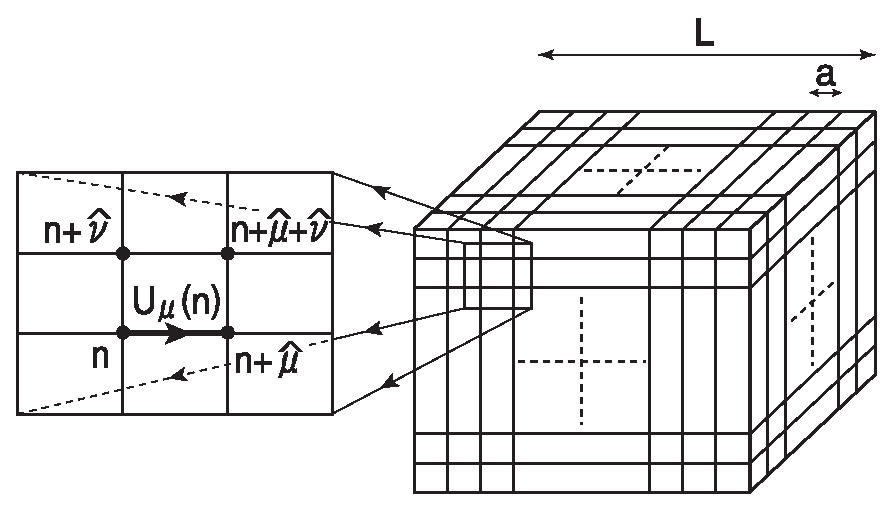
\includegraphics[scale=0.6]{Chapter3-figures/cube.eps}
 \end{center}
\caption{A hypercubic lattice in Euclidean spacetime with
 a lattice constant $a$ and the lattice size $L$.
 Quarks $q(n)$ (gluons $U_{\mu} (n)$ ) are
 defined on the sites (links).}
\label{fig:cube}
\end{figure}
%%%%%%%%%%%%%%%%%%%%%%%%%%%%%%


Let us consider a four dimensional  hyper-cubic lattice
 with a lattice spacing $a$ and the four dimensional volume $L^4$.
 Each lattice site is specified by  $n_{\mu}$ corresponding to the
 Euclidean coordinates through $x_{\mu} = a n_{\mu}$ (see Fig.\ref{fig:cube}).
   The {\it link variable} (the shortest  Wilson line on the lattice) is an SU(3)
 matrix connecting the neighboring sites $n$ and $n + \hat{\mu}$,
\beq
\label{eq:5.wilson-link}
U_{\mu}(n) = {\rm exp} \left(  ig a A_{\mu} (n) \right) .
\eeq
 Here $\hat{\mu}$ implies a vector  pointing the 
 direction of $\mu$ with a length $a$. 
 Since it is the minimal
     Wilson line, we do not need the path ordering symbol ${\rm P}$.
   Also, any non-minimal Wilson line on the lattice  is represented by a
    product of link-variables.  For later purpose, we introduce the link variable pointing the 
    opposite direction as  $U_{-\mu}(n+\hat{\mu}) = [U_{\mu}(n)]^{\dagger}$.

Let us now  define the smallest closed loop;
\beq\label{eq:5.wilson-plaq}
 U_{\mu \nu}(n) = 
 U_{\nu}^{\dagger}(n) U_{\mu}^{\dagger}(n+ \hat{\nu} ) 
  U_{\nu}(n+ \hat{\mu} )U_{\mu}(n ).
\eeq
Under local gauge
 transformation (rotation under  arbitrary  SU(3) matrix $V(n)$), we have 
\beq
 U_{\mu}(n) \rightarrow  V(n) U_{\mu}(n) V^{\dagger}(n+\hat{\mu}), \ \ 
 U_{\mu \nu}(n) \rightarrow  U_{\mu \nu}^V(n)=V(n) U_{\mu \nu}(n) V^{\dagger}(n),
 \eeq
which are the  direct consequence of Eq.(\ref{eq:5.wilson-line-iii}).

In the naive continuum limit where $a \rightarrow 0$, we have
\beq
 \label{eq:5.wilson-plaq-cont}
 U_{\mu}(n) -1 
   &=& iga A_{\mu}(n)  + O(a^2), \\
 \label{eq:5.wilson-plaq-cont-2}
 U_{\mu \nu}(n) -1 
  &=& \exp \left( iga^2 t^b (G_{\mu \nu}^b(n) + O(a^3) ) \right) -1
  = ig a^2 G_{\mu \nu}(n)  + O(a^4), \\
{\rm tr} \left(    U_{\mu \nu}(n) -1 \right) 
 &=&   {\rm tr} \left[  iga^2 t^b (G_{\mu \nu}^b(n) + O(a^3)) - \frac{1}{2} g^2 a^4 G_{\mu \nu}(n)^2 + O(a^5) \right] \nonumber \\ 
 &=& - \frac{1}{4} g^2 a^4 (G_{\mu \nu}^b(n))^2 + O(a^5) .
\eeq
Here  Eq.(\ref{eq:5.wilson-plaq-cont-2}) is obtained by 
 using the Baker-Campbell-Hausdorff formula, 
  ${\rm exp}X\cdot {\rm exp}Y =
  {\rm exp}(X + Y + [X,Y]/2 + \cdot \cdot \cdot )$.  (Exercise \ref{prob:2}). 


Finally, 
a  gluon action on the lattice, which reduces to the Yang-Mills
 action in the leading order of the  naive continuum limit ($a \rightarrow 0$), reads
\beq
\label{eq:5.wilson-action-cont}
 S_{\rm G}  &=& \beta \sum_{\rm Pl} \left[ 1 - \frac{1}{N_c} {\rm Re} \ {\rm tr} \ U_{\mu \nu}(n) \right] \\
 &=& \beta  a^4 \sum_n \sum_{\mu < \nu} \left[ 1 - \frac{1}{2N_c} {\rm tr}  \left( U_{\mu \nu}(n) +  U_{\mu \nu}^{\dagger}(n) \right) \right] \nonumber \\
 & = & \frac{1}{g^2} \sum_n \sum_{\mu \neq \nu} {\rm tr} \left[ 1 -U_{\mu \nu} (n) \right] 
  \ \ \ \ \xrightarrow{a\rightarrow 0}   \ {1 \over 4} \int d^4x  \ G_{\mu \nu}^b (x)^2 , \nonumber
 \eeq
where $\sum_{\rm Pl} $ is a sum over all non-oriented {\it plaquettes} (minimum square tile on the lattice with the area $a^2$). 
Note that  $\beta \equiv \frac{2N_c}{g^2}$ with $N_c$ being the number of colors ($N_c=3$ for QCD) 
 should not be  confused with the inverse temperature. 
    The lattice gluon action is not unique in the sense
 that one may add arbitrary non-minimal terms which vanish
 in the continuum limit ($a\rightarrow 0$).
  
%============================
\subsection{Lattice fermions}
%============================

There exist three types of gauge invariant objects made of nearest neighbor fermions as shown in Fig.\ref{fig:wilson-line}(b);
\beq
\label{eq:5.nn-link}
\bar{q}(n) q(n), \ \ 
\bar{q}(n+\hat{\mu}) U_{\mu}(n) q(n), \ \
\bar{q}(n-\hat{\mu}) U_{-\mu}(n) q(n).
\eeq
Here one may put any $\gamma$-matrices  between $\bar{q}$ and $q$
 without spoiling the color gauge invariance.
A special combination of the above   terms is called the Wilson's fermion action 
\beq
\label{eq:5.wilson-fermion}
\! \! \! 
S_{\rm F}
 &=& a^4 \sum_n 
  \left[
    m   \bar{q}(n)q(n) - \frac{1}{2a}
    \sum_{\pm \mu} \bar{q}(n+\hat{\mu}) {\Gamma}_{\mu} U_{\mu}(n) q(n)   
    - \frac{r}{2a} \sum_{\pm \mu}   \left( \bar{q}(n+\hat{\mu}) U_{\mu}(n) q(n) - \bar{q}(n)q(n) \right) 
  \right]  \nonumber \\ 
\label{eq:5.wilson-fermion2}
 & \equiv & a^4 \sum_{n',n} \bar{q}(n')
 \left( m \delta_{n',n} + D_{_{\rm W}}(n',n;U) \right) q(n)  \\
 \label{eq:5.wilson-fermion3}
 & & \xrightarrow[a \rightarrow 0] \ \  \int d^4x\  \bar{q} (x)  \left(\Gamma_{\mu} D_{\mu} + m - \frac{ar}{2} D_{\mu}^2 \right)   q(x),
\eeq
where the Wilson's Dirac operator in Eq.(\ref{eq:5.wilson-fermion2})  with the Wilson's parameter $r$ reads
\beq
\label{eq:5.wilson-dirac}
D_{\rm W}(n',n;U) 
  = - \frac{1}{2a} \sum_{\pm \mu}
 \left[
 \delta_{n',n+\hat{\mu}} (r+ {\Gamma}_{\mu} ) U_{\mu}(n)
   - r \delta_{n',n}
 \right]      .
\eeq
 To take the continuum limit in Eq.(\ref{eq:5.wilson-fermion3}), 
we use  the midpoint prescription,  $(f(x+a)-f(x-a))/2a = f'(x) + O(a^2)$
 and $(f(x+a)+f(x-a) -2f(x))/a^2 = f''(x) + O(a^2)$.
 One of the important properties of $ D_{\rm W}(n',n;U) $ is its $\Gamma_5$ Hermiticity (Exercise  \ref{prob:3}),
 \beq
 \label{eq:gamma5-hermite}
 \Gamma_5 D_{\rm W} \Gamma_5 = D_{\rm W}^{\dagger},
 \eeq
where $\Gamma_5$ is given in Appendix [Four vectors and Dirac matrices].  Note that the 
 Hermitian conjugate is taken for color, spin and  spacetime.
 
The dispersion relation (relation between the energy and momentum)
for free fermion can be obtained from Eq.(\ref{eq:5.wilson-fermion}) by taking $U_{\mu}=1$ (or equivalently $g=0$)
and substituting  the Fourier transform,
$q(n) = \int_{-\pi/a}^{\pi/a} \frac{d^4p}{(2\pi)^4} e^{i p_{\mu} n_{\mu}} q(p)$.
 This leads to $S_{\rm F}^{\rm (free)}= \int \frac{d^4p}{(2\pi)^4} \bar{q}(-p) {\cal G}_{\rm F}^{-1} q(p)$ with the
 free fermion propagator (Exercise  \ref{prob:4}),
 \beq
 \label{eq:DF}
 {\cal G}_{\rm F} (p) &=& \frac{-i  \sum_{\mu} \bar{p}_{\mu} \Gamma_{\mu}  + m(p) }{\sum_{\mu} \bar{p}_{\mu}^2 + m^2(p)},  \\
 \label{eq:Mp}
 \ \ \ \ \bar{p}_{\mu} &=& \frac{1}{a} \sin (p_{\mu} a), \ \  m(p)  =  m(0) + \frac{r}{a}  \sum_{\mu}      \left( 1-\cos (p_{\mu} a) \right)  .
 \eeq
Since $\sin (p_{\mu} a)$ becomes zero
 for $p_{\mu}a$=$(0,0,0,0)$, $(\pi, 0,0,0)$,$ \cdot $
  $(0,\pi,\pi,\pi)$, $(\pi,\pi,\pi,\pi)$, there arise
  $2^4 =16$ degenerate fermions  if we take  $r=0$.
 This is called the fermion doubling problem on the 
 lattice. In fact, there is a no-go theorem
 by  Nielsen and Ninomiya: 
 The  fermion doubling always exists, if the free fermion action  on the lattice
 has (i) bilinearity in quark field, 
  (ii) translational invariance,
   (iii) hermiticity (in the Minkowski spacetime),
    (iv) locality in spacetime, and (v) exact chiral symmetry.
Indeed, (i)-(v) are all satisfied for $r=0$.

The doubling in the dispersion relation in  the Minkowski spacetime is easily seen by Wick rotating 
$p_4 \rightarrow i E$ in Eq.(\ref{eq:DF}).  As an illustration, let us take the case with massless fermion ($m(0)=0$)
in (1+1)-dimension.  Then, the zero of the denominator after the Wick rotation for small $a$ gives,
\beq
E^2(p) \simeq \left( \frac{1}{a} \sin (pa) \right)^2 + \left( \frac{r}{a}  (1-\cos(pa)) \right)^2 ,
\eeq
whose positive energy solution is plotted in Fig.\ref{fig:dispersion} for several values of $r$.
One finds that the unphysical massless pole at $pa=\pi$ is lifted up as $r$ increases.

% FIG %%%%%%%%%%%%%%%%%%%%%%%%%%
\begin{figure}[t]
\begin{center}
%\framebox[74mm]{\rule[-26mm]{0mm}{52mm}}
\includegraphics[scale=0.75]{Chapter3-figures/dispersion.eps}
 \end{center}
\caption{The  dispersion relation for massless fermion in (1+1)-dimension on the lattice for different values of 
 the Wilson's parameter $r$.  The linear dispersion in the continuum ($E=p$) is also shown for comparison.}
\label{fig:dispersion}
\end{figure}
%%%%%%%%%%%%%%%%%%%%%%%%%%%%%% 
 
 In general, $r\neq 0$  leads to a mass splitting   of 16 fermions:
$    m(p)  \simeq  m(0)\  (^{\forall }p_{\mu} \rightarrow 0) $ and 
$m(p)= m(0) +  \frac{2r}{a}N_{\pi}  \   (^{\exists }p_{\mu} \rightarrow \pi/a) $,
 where $N_{\pi}(=1,2,3,4)$ being the number of $\pi$'s
 in  $p_{\mu}a$.  This implies that we can select only one light
 fermion by choosing $m(0) \simeq 0$ and all the other
 15 fermions have masses of $O(1/a) $  for positive  $r$.  
 A price to pay  is that the non-vanishing  $r$ breaks chiral symmetry
 explicitly for finite $a$, i.e. $\{ \gamma_5, D_{\rm W} \} \neq 0$ even for $m(0)=0$.   
  Namely, the Nielsen-Ninomiya's no-go theorem is evaded by breaking the condition (v).

  Better way to  evade the no-go theorem 
  is to break the condition (v)  in a way that the definition of
 chiral symmetry is modified.  
 Suppose we consider a modified chiral rotation in the flavor space,
 \beq
 \label{eq:5.mod-chiral}
 q \rightarrow   {\rm e}^{-i \theta_{\rm {_A}} \hat{\Gamma}_5   } q, 
  \ \ \bar{q} \rightarrow \bar{q} {\rm e}^{-i \theta_{\rm {_A}} \Gamma_5 }  \ \ 
   {\rm with} \ \  \hat{\Gamma}_5 =  \Gamma_5 (1-2 a D_{_{\rm GW}})  ,
\eeq
which  reduces to the standard axial rotation for $a\rightarrow 0$.
Here  $D_{\rm GW}$ is a generalized Dirac operator which is 
 constructed so that   
  $\bar{q} D_{\rm GW} q$ is  invariant under
 Eq.(\ref{eq:5.mod-chiral}) even for finite $a$;
\beq
 \label{eq:5.GW-1}
\Gamma_5 D_{\rm GW} + D_{\rm GW} \hat{\Gamma}_5 =0 ,
\eeq
or equivalently  $\{ \Gamma_5, D_{_{\rm GW}} \} 
 = 2a D_{_{\rm GW}} \Gamma_5 D_{_{\rm GW}}$.
 This     is called the Ginsparg-Wilson relation.
  An explicit form of $D_{\rm GW}$ may be constructed as
\beq
 \label{eq:5.overlap-op}
 D_{\rm GW} = 
 \frac{1}{2a} \left( 1+  \frac{X}{\sqrt{X^{\dagger}X}} \right)  \ \  
 {\rm with} \ \ 
 X \equiv   D_{\rm W}^{(r=1)} - m_0  ,
\eeq
where $m_0 a$ being a dimensionless parameter of $O(1)$.
 Unlike the case of $m$ in the Wilson fermion,
 $m_0$  is not directly related to the physical fermion mass.
 Nevertheless,  if we choose the region $0< m_0 a < 2$,  
  there exists
 an  exact massless mode for $N_{\pi}=0$ for finite $a$,
 and  other 15 modes have a large mass 
 $(2/a)(2N_{\pi}-m_0 a)>0$.   (Exercise  \ref{prob:5}).
 
 Going back to the Wilson's fermion action, Eq.(\ref{eq:5.wilson-fermion}).
it  can be  conveniently rewritten  as 
\beq
 \label{eq:5.wilson-fermion-lat}
S_{\rm F}    
    & = & \sum_{n',n} \bar{\psi}(n') F(n',n;U) \psi(n) ,\\
\label{eq:5.wilson-fermion-op}
F(n',n;U) &=& \delta_{n'n} 
- \kappa \sum_{\pm \mu} \delta_{n',n+\hat{\mu}}
 (r + {\Gamma}_{\mu}) U_{\mu}(n),
\eeq
where we have redefined the quark field 
 as $\psi = a^{3/2} q /\sqrt{2\kappa }$ with
 $\kappa = [2(ma + 4r)]^{-1}$
 being the  {\it hopping parameter}. 
  If the quark mass $m$ is large, $\kappa$ is
 small and the ``hopping" to the 
  neighboring lattice site is suppressed.
   
%=================================
\subsection{Partition function on the lattice}
%=================================

The functional integration over quarks and gluons in continuum QCD
in Eq.(\ref{eq:Z-QCD}) is now transformed to the integration over quarks 
  on each site and gluons on each link in lattice QCD. 
 With Eq.(\ref{eq:5.wilson-action-cont}) and
   Eq.(\ref{eq:5.wilson-fermion-lat}), the partition function without the external field ($J=0$) reads
\beq
\label{eq:5.lattice-Z}
{\cal Z}  =  \int[dU d\bar{\psi}d\psi]   {\rm e}^{-  S_{\rm G}(U) - S_{\rm F}(\bar{\psi},\psi,U) }  
    =  \int[dU]\ {\rm Det}\ F(U) \ {\rm e}^{- S_{\rm G}(U) }
    = \int[dU]\  \ {\rm e}^{- S_{\rm eff}(U) }
\eeq
To obtain the second equality, we have explicitly carried out the integration over the
 Grassmann variables, $\bar{\psi}$ and $\psi$, 
 by using the formula in Appendix [Gaussian and Grassmann integrals]. Here ${\rm Det}$ implies the determinant in 
  spacetime, color, flavor and spin degrees of freedom.
In the third equality, the exponent  is defined as 
 \beq
\label{eq:Seff}
 S_{\rm eff}(U) \equiv S_{\rm G}(U) - {\rm ln Det} F(U).
 \eeq
 
 The integration over the group element $[dU] = \prod_{\mu,n} dU_{\mu}(n) $ can be defined through 
  the {\it Haar measure} $dU$ which has the property,
  $ d(V_{\rm L}U V_{\rm R}^{\dagger})=dU$
  with  $V_{\rm L,R}$ being arbitrary group elements. Such a measure is
   unique for compact groups such as SU$(N)$.
 If we parametrize the group element as $U=\exp(i \theta_a t^a)$,  one can define the 
 distance in the group space as $ds^2 = g_{ab}  (\theta) d\theta_a d\theta_b$, where the 
 metric is given by $g_{ab}=  {\rm tr} (L_aL_b) =  {\rm tr} (R_a R_b) $ with 
 \beq
 \label{eq:LR-form}
 L_a= -i U^{-1} ( {\partial} U/{\partial \theta_a}), \ \ \ 
 R_a= -i ({\partial}U/{\partial \theta_a} ) U^{-1}.
 \eeq   
 Then the Haar measure can be   explicitly written as
  \beq
  \label{eq:Haar-measure}
   dU = {\cal N} \sqrt{ \det g} \ \prod_a d\theta_a,
  \eeq
  with an overall normalization factor ${\cal N}$.
  
 The followings are some examples of the  SU($N$)  group integration, which can be proved
 by the invariant property of the Haar measure (except for the first one which determines the 
 normalization of the measure) (Exercise \ref{prob:6}):
 \beq
 \label{eq:group-int-0}
  & &   \int dU \  1  =  1 , \\ 
 \label{eq:group-int-1}
 & &   \int dU \ U_{ij}  =  0, \\
 \label{eq:group-int-2}
 & &    \int  dU \ U_{ij} U_{k\ell}^{\dagger}  =  \frac{1}{N} \delta_{i\ell} \delta_{jk} , \\
 \label{eq:group-int-4}
 & &  \int dU \ U_{ij} U_{k\ell}  U_{i'j'}^{\dagger} U_{k'\ell'}^{\dagger}
 = \frac{ \delta_{ij'} \delta_{ji'} \delta_{k\ell'} \delta_{\ell k'} + {(j' \leftrightarrow \ell',  i' \leftrightarrow k' ) }}{N^2-1}
   -  \frac{\delta_{ij'} \delta_{jk'} \delta_{k\ell'} \delta_{\ell i'} + { (j' \leftrightarrow \ell',  i' \leftrightarrow k' )}  }{N}, \\
 \label{eq:group-int-B}
 & &  \int dU \ U_{i_1 j_1} \cdots U_{i_N j_N} = 
 \frac{1}{N!} \epsilon_{i_1 \cdots i_N}    \epsilon_{j_1 \cdots j_N} .
 \eeq    

   
Similar to the statistical systems such as the Ising model, 
 observables are obtained by averaging over the statistical weight  as
 \beq
 \langle {\cal O} \rangle = \frac{1}{{\cal Z}}  \int[dU]\ {\cal O}(U) \ {\rm e}^{- S_{\rm eff}(U) }.
 \eeq
    Due to the gauge invariance of the Haar  measure,
 gauge non-invariant quantities have vanishing expectation values
  (Elitzer's theorem).  For example, consider the expectation value of the link variable,
 \beq
 \label{eq:elitzer}
 \langle U_{\mu} (n) \rangle 
 = \frac{1}{{\cal Z}}  \int [dU] U_{\mu} (n)  \ {\rm e}^{- S_{\rm eff}(U) }  = V(n)  \langle U_{\mu} (n) \rangle ,
\eeq
where we have made a change of variable, $U_{\mu}(n) \rightarrow V(n) U_{\mu}(n)$ with $V(n)$ 
being the $SU(N)$ matrix, and used the  gauge invariance of the Haar measure as well as ${\rm Det}\ F(U)$ and 
$S_{\rm G}(U)$.  Since Eq.(\ref{eq:elitzer}) must be true for arbitrary $V(n)$, we have $ \langle U_{\mu} (n) \rangle =0$.
 
Some examples of the non-vanishing  observables are shown  in Fig.\ref{fig:correlation}:
 (a) and (b) correspond to the mesic and baryonic correlations, respectively,  while (c) is a correlation related to the 
baryon-baryon interactions.  The filled circles are the spacetime points where the quarks and anti-quarks
are created or absorbed. Each  line with arrow indicates the quark propagator $F^{-1}(n,n';U)$ 
connecting two spacetime points $n$ and $n'$.  Thus, the explicit forms of the
 mesic and baryonic correlations are
 \beq
 \label{eq:correlation-M}
C_{\rm M}(n,n') 
 &=& \frac{1}{{\cal Z}}  \int [dU] \ F_{\alpha \beta}^{-1}(n,n';U) F_{\beta \alpha}^{-1}(n',n;U)  \ {\rm e}^{- S_{\rm eff}(U) } ,\\
\label{eq:correlation-B}
C_{\rm B}(n,n') 
 &=& \frac{1}{{\cal Z}}  \int [dU] \ \epsilon_{\alpha \beta \gamma} \epsilon_{\alpha' \beta' \gamma'} 
 F_{\alpha \alpha'}^{-1}(n,n';U) F_{\beta \beta'}^{-1}(n,n';U) F_{\gamma \gamma'}^{-1}(n,n';U)  \ {\rm e}^{- S_{\rm eff}(U) } ,
  \eeq
where all the color indices are contracted so that $C_{\rm M}$ and $C_{\rm B}$ are gauge invariant. 
 Other quantum numbers such as spin and flavor  associated with $F^{-1}$ are
 not shown explicitly.
  Spacetime, spin and flavor dependences of  $C_{\rm M}(n,n')$ in (a) and $C_{\rm B}(n,n')$ in (b)
  have all the information on the hadronic states in various different channels, while
  $C_{\rm BB}(n,m,n',m')$   in (c) has the information on baryon-baryon interactions.
      
% FIG %%%%%%%%%%%%%%%%%%%%%%%%%%
 \begin{figure}[t]
%\vspace{-1cm}
\begin{center}
%\framebox[74mm]{\rule[-26mm]{0mm}{52mm}}
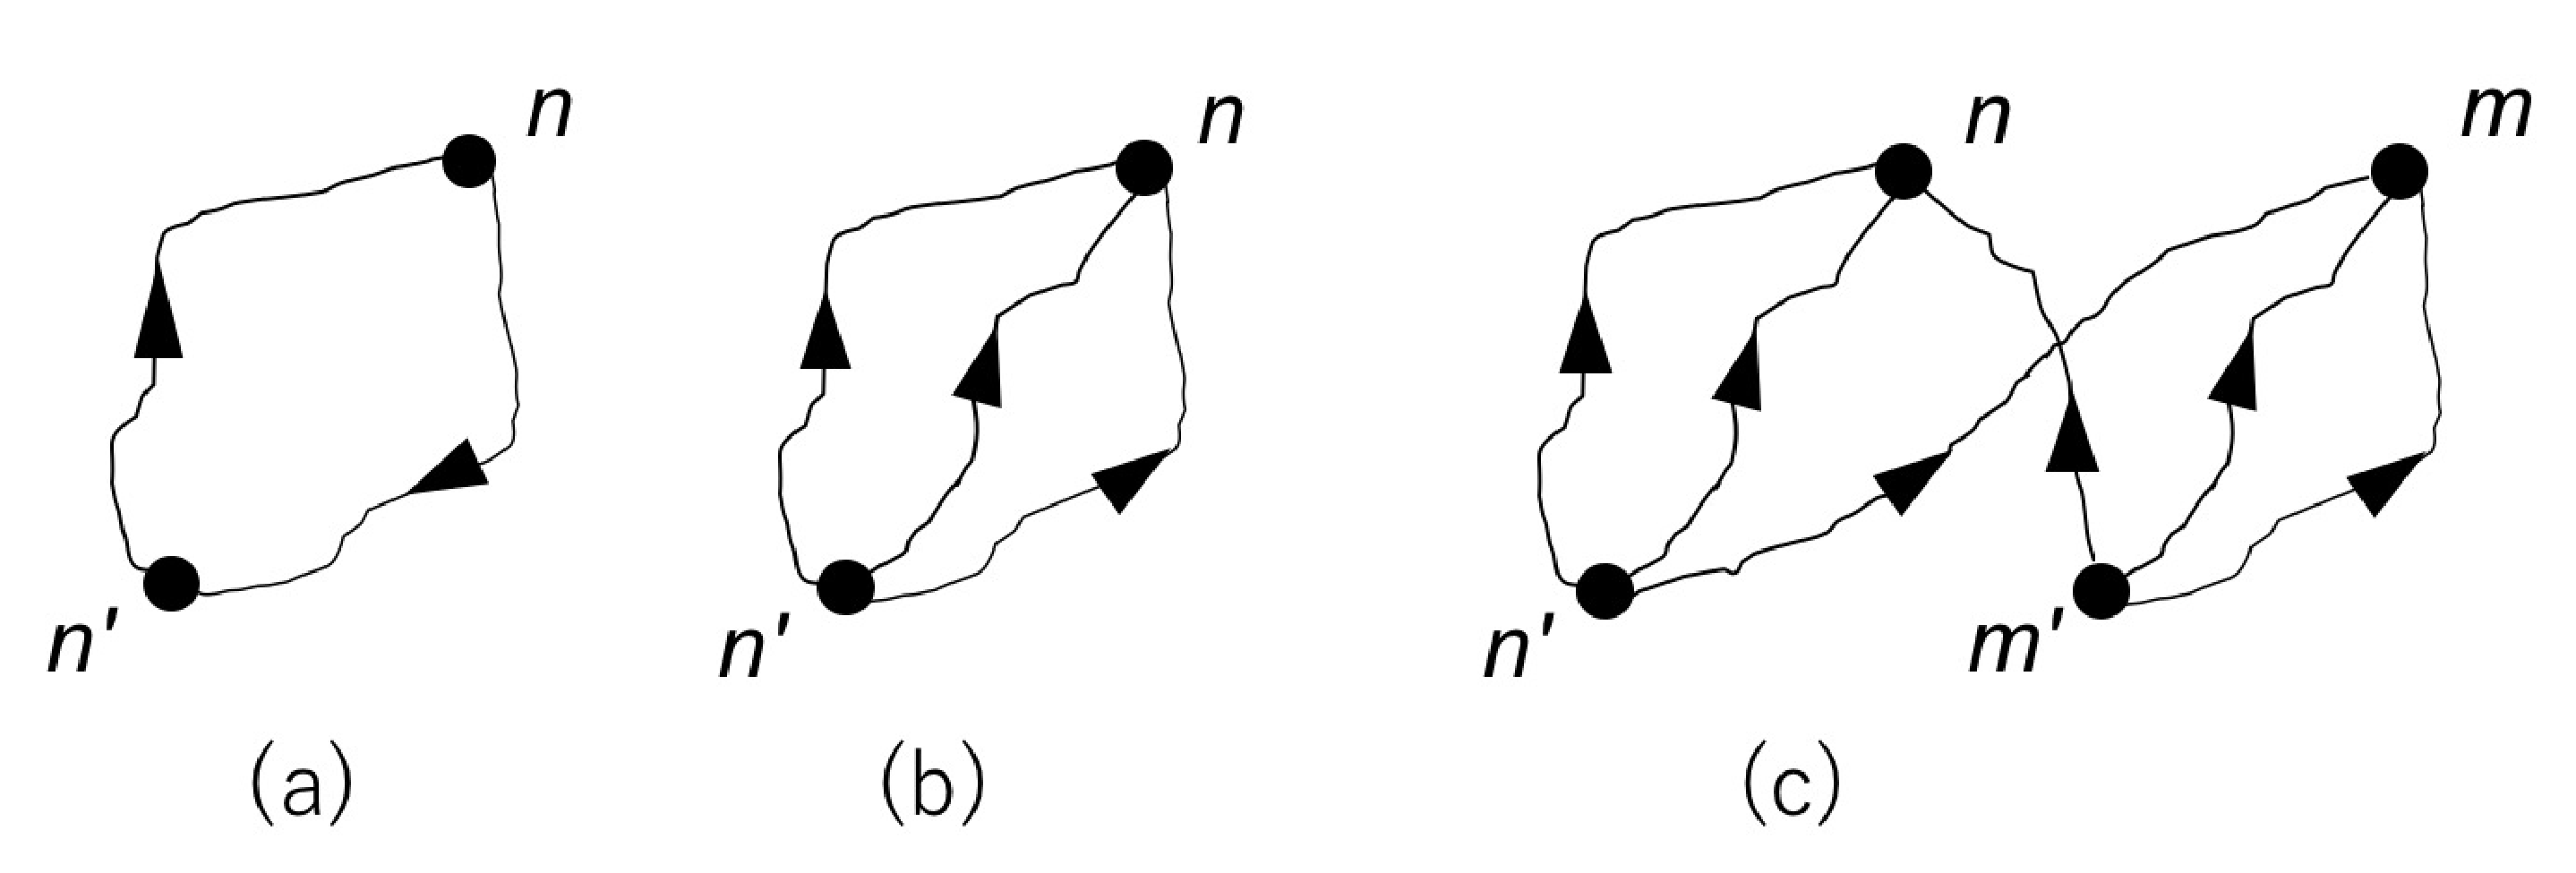
\includegraphics[scale=0.2]{Chapter3-figures/correlations.eps}
 \end{center}
%\vspace{-1cm}
\caption{
(a) Single meson correlation representing the propagation of a  meson created at point $n'$ and absorbed at point $n$.
(b)  Single baryonic correlation representing the propagation of a  baryon created at point $n'$ and absorbed at point $n$.
(c)  Two baryon correlation which contains the information on baryon-baryon interaction.}
\label{fig:correlation}
\end{figure}
%%%%%%%%%%%%%%%%%%%%%%%%%%%%%%%
 
   
%===========================================
\subsection{Strong coupling expansion and quark confinement}
%===========================================


% FIG %%%%%%%%%%%%%%%%%%%%%%%%%%
\begin{figure}[t]
\begin{center}
%\framebox[74mm]{\rule[-26mm]{0mm}{52mm}}
\includegraphics[scale=0.55]{Chapter3-figures/wilson-L.eps}
 \end{center}
\caption{A rectangular  Wilson loop with the
 temporal (spatial) size ${\cal T}$ ($R$).}
\label{fig:wilson-L}
\end{figure}
%%%%%%%%%%%%%%%%%%%%%%%%%%%%%%

One of the remarkable properties of QCD is the   confinement of quarks inside 
hadrons.  Simplest setup to see this phenomena is to consider
the potential $V(R)$ between  an infinitely heavy quark $Q$ and an anti-quark $\bar{Q}$ with
a fixed separation $R$.
It corresponds to Fig.\ref{fig:wilson-L} and can be written as
\beq
 \label{eq:5.wilson-loop-lattice}
\langle W(C) \rangle  
 & = & \langle {\rm tr}\ \prod_{{\rm link}\in C}  U_{\mu}(n) \rangle , \\
 \label{eq:5.wilson-loop-asym}
 & \propto  & 
  {\rm e}^{-V(R) {\cal T} } \simeq 
 \exp \left[ -\left( K R + b + \frac{c}{R} + \cdots \right) {\cal T} \right] ,
\eeq  
where we  have taken a limit     
${\cal T} \gg R \rightarrow \infty$ in   Eq.(\ref{eq:5.wilson-loop-asym}).
 Remembering the fact that the real time $t$ and the imaginary time $\tau$ are
 related as  $\tau=it$, the exponential falloff of  $\langle W(C) \rangle$ in $\tau$ implies the 
  temporal oscillation in $t$, and its $R$-dependent coefficient is nothing but the 
 interaction  energy between $Q$ and $\bar{Q}$.  
 
In Eq.(\ref{eq:5.wilson-loop-asym}), 
   $K > 0$  implies 
 the existence of a string-like
linear confining potential.
 It also implies 
 the area law  of the Wilson loop 
 $\langle W(C) \rangle \sim \exp(-K{\cal A})$
 where ${\cal A}= R \times {\cal T} $ is 
  the area inside the path $C$.
    In full QCD where pair creation of light quarks 
 are allowed,  
  the linear rising potential becomes eventually 
    flat at long distances due to the breaking of the string,
  $Q\bar{Q} \rightarrow (Q\bar{q})(q\bar{Q})$.
  
  To make the analysis simple, let us now consider the 
  SU$(N_c)$ Yang-Mills theory
  without light quarks: This is called the quenched 
  approximation and corresponds to take $F(U) =1$.
In this case,  the Wilson loop can be evaluated analytically
 in the strong coupling regime ($g \rightarrow \infty$).
First of all,  $S_{\rm G}$ is proportional to $1/g^2$,
so that  one can make an expansion,  
$\exp (-S_{\rm G}) = 1 - S_{\rm G}+ S_{\rm G}^2 /2 + \cdots $
 and finds (Exercise \ref{prob:7})
\beq
\label{eq:5.wilson-strong}
\langle W(C) \rangle = {1 \over {\cal Z}}
 \int [dU] \ {\rm tr} \prod_{{\rm link}\in C} U_{\mu}(n) \  
 \sum_{\ell =0}^{\infty} \frac{1}{\ell !} (-S_{\rm G})^{\ell}.
\eeq
 
Only the first three integrals, Eqs.(\ref{eq:group-int-0},\ref{eq:group-int-1},\ref{eq:group-int-2}),
 are necessary to extract the leading contribution to 
 $\langle W(C) \rangle $  in the strong coupling.
   Key observation is that all the $U$'s 
  from the Wilson loop and $U^{\dagger}$'s 
 from $(-S_{\rm G})^{\ell}$ should be paired in the leading order of $1/g^2$
 in   Eq.(\ref{eq:5.wilson-strong}).
  This means that the area inside the Wilson loop is tiled up 
 with minimum number of plaquettes as shown in
  Fig.\ref{fig:strong-c}. All the structures other than 
  the minimal surface are higher orders in  $1/g^2$.

% FIG %%%%%%%%%%%%%%%%%%%%%%%%%%
 \begin{figure}[t]
\begin{center}
%\framebox[74mm]{\rule[-26mm]{0mm}{52mm}}
\includegraphics[scale=0.65]{Chapter3-figures/strong-c.eps}
 \end{center}
\caption{A minimum surface in which the Wilson loop is tiled 
   up by the fundamental plaquettes in the 
 strong coupling limit.}
\label{fig:strong-c}
\end{figure} 
%%%%%%%%%%%%%%%%%%%%%%%%%%%%%%

 In the evaluation of the numerator of
 Eq.(\ref{eq:5.wilson-strong}), 
 each plaquette has a contribution $1/g^2$. 
 Also each  integration on the link
   gives a factor $1/N_c$
   and the contraction of the color indices gives a factor $N_c$
 on each  site.
  On the other hand,
 ${\cal Z}$  (the denominator of Eq.(\ref{eq:5.wilson-strong})
 is   unity in the leading order. 
    Thus, one arrives at the formula in the lowest order
 of the strong coupling expansion,
\beq
 \label{eq:5.strong-estimate}
\frac{1}{N_c} \langle W(C) \rangle 
& & \xrightarrow[g^2\rightarrow \infty] 
 \  \frac{1}{N_c} \cdot  
\left(\frac{1}{g^2} \right)^{N_{\rm plaq}} \cdot  
\left(\frac{1}{N_c} \right)^{N_{\rm link}} \cdot N_c^{N_{\rm site}}  , \nonumber \\
& & \ \ \ \ \ \ \ \ \ \ \ =\left(\frac{1}{N_c g^2} \right)^{\frac{R {\cal T}}{a^2}} 
= \exp \left( - \frac{\ln N_c g^2}{a^2} R {\cal T} \right) ,
\eeq
where we have used a relation, $N_{\rm link}-N_{\rm site}+1 
 = N_{\rm plaq}$ and 
$N_{\rm plaq} a^2 = R {\cal T} ={\cal A}$.
 Since it shows the area law, \index{area law}
  the confinement is naturally obtained in the strong coupling
  with the linear rising potential, 
\beq
 \label{eq:5.linear-potential}
V(R) = K R \ \ {\rm with} \ \ K = \frac{1}{a^2} \ln (N_c g^2).
\eeq

 If we consider higher orders of the strong coupling expansion,
   ``rough" surfaces should be taken 
 into account.
 Nevertheless, the confining feature is
 stable against small perturbations in $1/g^2$.
  In fact, there exits a theorem 
  that,  for sufficiently large $g$, the strong coupling expansion 
  converges and shows confinement for all compact gauge groups  
  in all spacetime dimensions.
  

  A question here is that whether the real world 
  corresponds to the strong coupling region discussed above.
  The answer is no;  the real world corresponds to  the weak coupling regime. 
  For compact QED (quantum electrodynamics
  formulated in terms of the  U(1) link variable),
  the confinement  $K>0$ in the strong coupling regime 
   changes to  $K=0$ in the weak coupling regime.
  On the other hand,  in QCD in four spacetime dimensions 
 with $N_c=3$,   the confinement feature is expected to persist even in the weak coupling regime. 
 Indeed, there are  strong evidences for this statement 
  from  LQCD simulations.
  Its analytic proof, however,  is  still missing and is being one of the 
   most challenging problems in mathematical  physics.
   

%===============================================
\subsection{Weak coupling expansion and continuum limit}
%===============================================

  Lattice QCD can be regarded as an effective field theory
   with an ultraviolet (UV)  cutoff in the coordinate space. 
   The gauge coupling  $g$ is then interpreted as
  a bare coupling defined at the scale $a$ where
  quantum fluctuations with the wave length shorter than 
  $a$ are integrated out.  In non-Abelian gauge theories,
   it can be shown that $g(a)$ decreases logarithmically as $a$ decreases
   unless the number of matter fields is not too large.  
    This is called the {\it asymptotic freedom}, and is essential for taking
    the continuum limit ($a \rightarrow 0$) to remove the 
    lattice artifact. 
        
 For simplicity, let us consider the case with massless fermions, where 
 observables
   ${\cal O}$ such as the string tension and the hadron masses  depend only
   on the coupling $g$ and the  regularization scale $a$. 
   Then,  from the dimensional ground, one can  write  
     \beq
\label{eq:5.O-dim}
 {\cal O} (g(a),a) = a^{-d} X(g(a)),
 \eeq
 where $d$ is the mass-dimension of ${\cal O}$ and $X$ is a dimensionless
 function of $g$.  The $a$-independence of the observable implies
 \beq
\label{eq:5.O-RG}
 a{d{\cal O} \over da} 
  =  
  \left( a \frac{\partial}{\partial a} 
 - \beta_{_{\rm LAT}}  \frac{\partial}{\partial g} \right) {\cal O}(g(a), a)  = 0 , 
\ \   \beta_{_{\rm LAT}}(g) =  -a {dg(a) \over da} .
\eeq
By integrating the first equation in Eq.(\ref{eq:5.O-RG}),  we find
\beq
\label{eq:5.lat-F}
 X(g) = 
 \exp \left( -d \int^g {dg' \over \beta_{_{\rm LAT}}(g')} \right) .
 \eeq
Suppose that 
 the beta-function can be expanded in terms of $g$ for small $a$:
$\beta_{_{\rm LAT}}(g)   = 
  - \beta_0 g^3 - \beta_1  g^5 + \cdot \cdot \cdot $. Here
  $\beta_0$ and $\beta_1$ can be shown to be independent of the 
   regularization scheme and are known to be 
\beq
\beta_0= \frac{1}{(4\pi)^2} \left( \frac{11N_c}{3}-\frac{2N_f}{3} \right),
\ \ \  \beta_1= \frac{1}{(4\pi)^4} \left( \frac{34N_c^2}{3}-\frac{38N_f}{3} \right),
\eeq
           for QCD with $N_c$ colors and     $N_f$ fermions.
  
% FIG %%%%%%%%%%%%%%%%%%%%%%%%%%
 \begin{figure}[t]
\begin{center}
%\framebox[74mm]{\rule[-26mm]{0mm}{52mm}}
%\includegraphics[scale=0.6]{as-scale.eps}
\includegraphics[scale=0.30]{Chapter3-figures/crossover.eps} 
 \end{center}
\caption{Crossover behavior of the dimensionless
 string tension $Ka^2$ from the strong coupling
 regime  $\beta=2N_c/g^2 \rightarrow 0$ to the weak coupling
  (asymptotic scaling) regime  $\beta=2N_c/g^2 \rightarrow \infty$
  for SU($N_c=2$) Yang-Mills theory.  The figure is adapted from
  \cite{Creutz:1980zw}.
  }
\label{fig:as-scale}
\end{figure}
%%%%%%%%%%%%%%%%%%%%%%%%%%%%%%%%

        
By integrating  the second equation in Eq.(\ref{eq:5.O-RG}) with the above expansion of
$\beta_{_{\rm LAT}}(g)$, one finds  
 \beq
\label{eq:5.a-vs-L}
 a = \Lambda_{_{\rm LAT}}^{-1} \cdot  
 \exp  \left( -\frac{1}{2\beta_0 g^2}  \right)  \cdot
  (\beta_0 g^2)^{-{\beta_1 \over 2 \beta_0^2}} 
 \cdot (1 + O(g^2)).
 \eeq
Here  $ \Lambda_{_{\rm LAT}}$ is called the scale parameter on the lattice, and  
   $g(a)$ can be expressed in terms of $a$ and $ \Lambda_{_{\rm LAT}}$ ((Exercise \ref{prob:8}),
 \beq
\label{eq:5.lat-running-g}
{1 \over g^2(a)} = \beta_0 \ln \left( 1 \over a^2  \Lambda_{_{\rm LAT}}^2 \right)
+ {\beta_1 \over \beta_0} \ln \ln \left( 1 \over a^2  \Lambda_{_{\rm LAT}}^2 \right)
+ \cdot \cdot \cdot .
\eeq
 This is the asymptotic freedom
 in which $g(a)$ decreases as $a$ decreases.  This also justified the 
 assumption that the beta-function can be expanded by $g(a)$ for small $a$.
 
 
Direct way to extract the actual value of $ \Lambda_{_{\rm LAT}}$  is to
 carry out  numerical simulations of  
 a certain physical quantity (such as the string tension)
 and compare the result with the experimental value. 
 For example, the string tension, which has mass-dimension
 two ($d=2$) should  behave as
\beq
\label{eq:5.lat-K}
K a^2 = C_K \exp \left( - {1 \over \beta_0 g^2} \right) 
(\beta_0 g^2)^{-\beta_1 /\beta_0^2} = C_K  \Lambda_{_{\rm LAT}}^2 ,
\eeq
with $C_K$ being a dimensionless numerical constant independent
 of $g$.  As  can be seen from this example, 
 the functional form of the physical quantities 
 for $g\sim 0$  is  severely constrained.  
This is called the {\em asymptotic scaling} which 
 is used to check whether the system is 
  close enough to the continuum limit.
Shown in Fig.\ref{fig:as-scale} is a historic numerical study, which shows 
 a crossover of $Ka^2$  from the strong coupling regime to the weak coupling regime
 in SU(2) Yangs-Mills theory. 
  


%===============================
\subsection{Running coupling}
%===============================

% FIG %%%%%%%%%%%%%%%%%%%%%%%%%%
\begin{figure}[t]
\begin{center}
%\framebox[74mm]{\rule[-26mm]{0mm}{52mm}}
%\includegraphics[scale=0.6]{as-scale.eps}
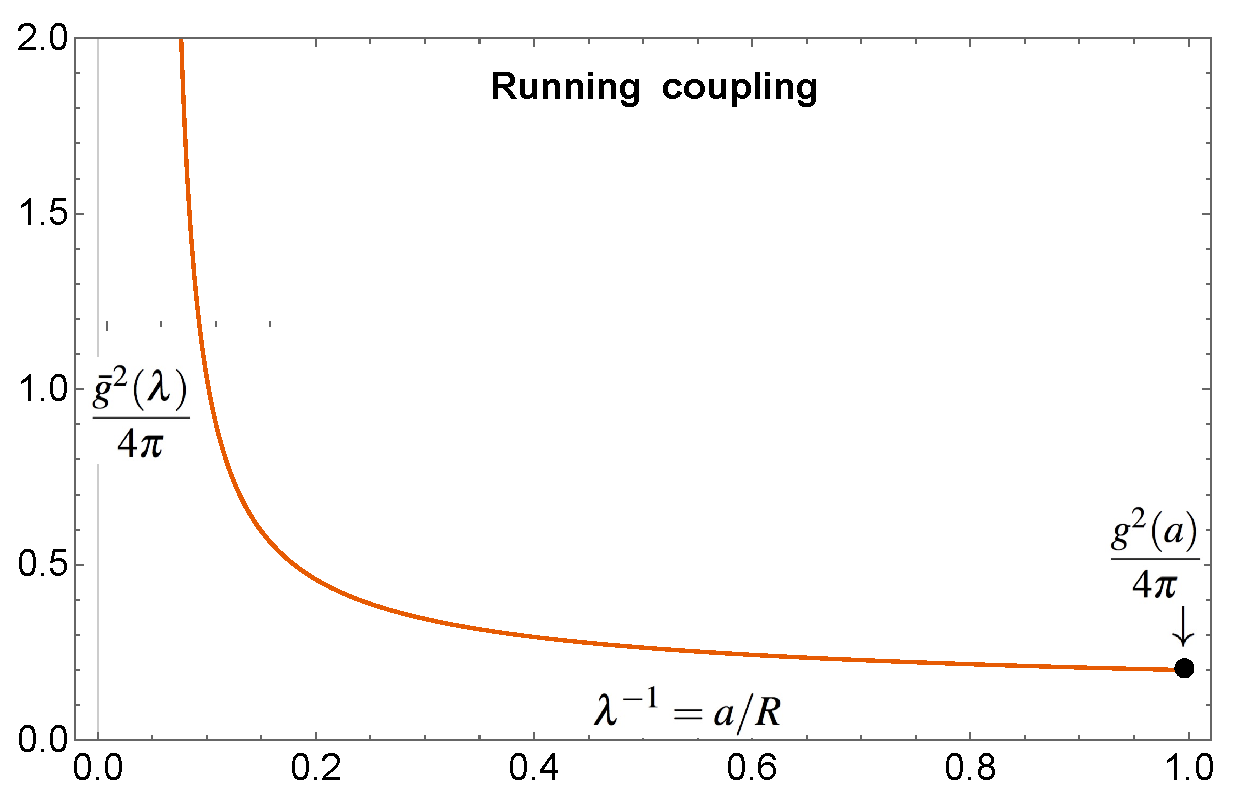
\includegraphics[scale=0.45]{Chapter3-figures/running-g.eps} 
 \end{center}
\caption{Perturbative running coupling $\frac{1}{4\pi}\bar{g}^2(\lambda)$ as a function of $\lambda^{-1}$.
In the short distance limit ($\lambda =1$), the running coupling coincides with the bare coupling $\bar{g}(\lambda=1)=g(a)$,
while, in the long distance regime ($\lambda \ll 1$), the running coupling grows. }
\label{fig:running-g}
\end{figure}
%%%%%%%%%%%%%%%%%%%%%%%%%%%%%%%


Let us now consider an observable ${\cal O}$ which depends 
not only on $g(a)$ and $a$ but also on some external dimensionful parameter.
For concreteness, we consider the heavy quark potential $V(R; g(a),a)$ in the 
quenched approximation.  Since it has the dimension of energy, one may write
\beq
V(R,g(a),a) = R^{-1} \tilde{V} (R/a, g(a)).
\eeq
Then the cutoff independence of the observable, $a \frac{d}{da}V(R,g(a),a)=0$,  leads to
\beq
\left( \lambda \frac{\partial}{\partial \lambda} + \beta_{_{\rm LAT}} \frac{\partial}{\partial g} \right) \tilde{V} (\lambda,g)=0,
\label{eq:RG-R}
\eeq
where we have introduced 
a dimensionless  scaling parameter $\lambda$ through $R=\lambda a$.

]The solution of the {\it renormalization group equation}, Eq.(\ref{eq:RG-R}), reads
\beq
\label{eq:RG-sol}
 \tilde{V} (\lambda,g(a)) = \tilde{V} (1, \bar{g}(\lambda)).
 \eeq
 Here $\bar{g}(\lambda)$ is called the {\it running coupling} which is  a solution of
\beq
\lambda \frac{d\bar{g}}{d\lambda}  = - \beta_{_{\rm LAT}} (\bar{g}(\lambda)),
\eeq
with the boundary condition, $\bar{g}(\lambda=1)= g(a)$.
One can show that  Eq.(\ref{eq:RG-sol})  satisfies Eq.(\ref{eq:RG-R}) explicitly by applying the partial derivatives 
 or more generally by the method of characteristics in Appendix [Method of characteristics].
Then, we eventually arrive at the formula 
\beq
V(R,g(a), a) = \frac{a}{R} V (a, \bar{g}(R/a), a) .
\eeq
If $R$ is  in the interval,  $a < R \ll  \Lambda_{_{\rm LAT}}^{-1}$, the running coupling $\bar{g}$ is small enough, so that 
one may use the perturbative expansion of $\beta_{_{\rm LAT}}$ to obtain
\beq
\bar{g}^2(R/a) \simeq \frac{g^2(a)}{1-2\beta_0 g^2(a) \ln (R/a)} =  \frac{1}{2\beta_0 \ln (1/(R \Lambda_{_{\rm LAT}}) ) }. 
\label{eq:running-R}
\eeq 
In Fig.\ref{fig:running-g}, the behavior of $\frac{1}{4\pi}\bar{g}^2(\lambda)$  as a function of $\lambda^{-1}$ is shown.
The bare coupling $\frac{1}{4\pi}g^2(a)$ appears as the boundary condition at shortest distance $\lambda=R/a=1$,
while $\frac{1}{4\pi} \bar{g}^2(\lambda)$ grows  as $\lambda$ increases.
The latter implies that the strong interaction has anti-screening feature.

For $R$ sufficiently close to $a$, one may evaluate the potential by using perturbation theory as
$V (a, \bar{g}(R/a), a)  = - C_{{\rm F}} \frac{\bar{g}(R/a)^2}{4\pi a}$, so that we finally obtain
\beq
\label{eq:RG-Coulomb}
V(R,g(a),a) \simeq - C_{{\rm F}} \frac{\bar{g}^2(R/a)}{4\pi R} \ \ \ \ \ (a < R \ll  \Lambda_{_{\rm LAT}}^{-1}),
\eeq
where $C_{{\rm F}}=4/3$ for $N_c=3$ is given in Appendix [SU($N$) algebra].
Eq.(\ref{eq:RG-Coulomb}) is nothing but the Coulomb potential with the running coupling constant.
Note that the left hand side is $a$-independent, while the right hand side has
logarithmic $a$-dependence through $\bar{g}$.  This is due to the use of perturbation theory;
such a logarithmic $a$-dependence  is cancelled by the next-to-leading order term.
Note also that the similar analysis can be done for any other observables.
The QCD thermal pressure at finite temperature $P(T,g(a),a)$ is a typical example, in which 
the weak coupling analysis (i.e. the description by  quark-gluon plasma picture)
is justified  under the condition  $  \Lambda_{_{\rm LAT}} \ll T < a^{-1}$. 



%%%%%%%%%%%%%%%%%%%
\section{Lattice QCD:  numerical simulations}
%%%%%%%%%%%%%%%%%%%


Suppose we have a lattice having $N_{\rm s}$ ($N_{\tau}$) number of sites
in each spatial (temporal) direction. Then 
 the total number of links is 
   $  N_{\rm s}^3 \times N_{\tau}  \times 4$. 
 Therefore the total  number of gluon integrations $\int [dU]$
 for a moderate lattice size  $N_{\rm s} = N_{\tau} =32$ reads
\beq
\label{eq:5.lattice-size}
 ( N_{\rm s}^3 \times N_{\tau} \times 4 )_{\rm links} \times 8_{\rm
 color} \sim 3 \times 10^7 .  
\eeq 
This is hopelessly a large number for standard methods of numerical
integration.  In this case, the Monte Carlo (MC) integration, which is
a statistical way to evaluate the integral, plays a powerful role. For
rapidly varying integrand, the MC integration should be supplemented
by the importance sampling to have better accuracy, in which the
rapidly varying part is sampled more than the slowly varying part.
     
     
 %==========================
\subsection{Importance sampling}
\label{ss:IS}
%==========================
    
     Let us consider the general partition function ${\cal Z}= \int [d\phi] \exp(-S(\phi)) $,
    with some c-number field $\phi$  and try to calculate  an observable ${\cal O} $ by
  \beq
  \langle {\cal O} \rangle = \frac{1}{{\cal Z}} \int [d \phi] \ {\cal O} (\phi) e^{-S(\phi)}.
  \eeq   
  The basic procedure of the MC integration
  with the {\it importance sampling} consists of two steps:
  \begin{enumerate}
  \item[(I)]   Generate a set of field configurations, $ \{  \phi^{(1)}, \phi^{(2)}, \cdots, \phi^{(N)} \}$, 
with $\phi^{(n)}$  being arranged to appear with 
 a probability in ``equilibrium", $W_{\rm eq}[\phi]={\cal Z}^{-1} \exp (-S(\phi))$.
 \item[(II)]  The field configurations thus generated 
 are  used to calculate the expectation value,
 \beq
\label{eq:5.obs-average}
\langle {\cal O} \rangle = \frac{1}{N}\sum_{n=1}^N {\cal O}^{(n)}
\pm \sqrt{{\sigma^2 \over N}}, \ \ \ \ \ 
\sigma^2 =  \frac{1}{N-1} \sum_{n=1}^N \langle {\cal O}^{(n)} - \langle {\cal O} \rangle \rangle^2 ,
\eeq
with ${\cal O}^{(n)}={\cal O}(\phi^{(n)})$.
\end{enumerate}

 %=========================================
\subsection{Markov chain Monte Carlo (MCMC)}
%==========================================
  
 For large  number of integration variables such as Eq.(\ref{eq:5.lattice-size}), 
 it  is essential to develop an appropriate scheme to carry out  Step (I) in Sec. \ref{ss:IS}. 
 The {\it Markov chain Monte Carlo (MCMC)}  method is one of such schemes. 
    
Let us consider a chain of configurations  generated successively starting from an
initial configuration,
\beq
\label{eq:M-chain}
 \phi_{0} \rightarrow  \phi_{1} \rightarrow \phi_{2}
 \rightarrow \cdots \rightarrow \phi_{i} \rightarrow  \phi_{i+1}
\rightarrow \cdots ,  
\eeq
where the ``{\it update}" of the $i$-th configuration ($\phi$)  to
the $(i+1)$-th configulation ($\phi'$)  is governed by the conditional probability
$P$ or equivalently  the transition matrix $\mathbf{T}$, 
\beq
\label{eq:M-transition}
P(\phi \rightarrow \phi') = (\mathbf{T})_{\phi \phi'} 
\eeq
which has the property, $\sum_{\phi'} P(\phi \rightarrow \phi')=1$.
Eq.(\ref{eq:M-chain}) generated by Eq.(\ref{eq:M-transition}) is called the {\it Markov chain} since
it is governed by the Markov process where the conditional probability depends only on the 
neighbouring pair. The probability distribution $W[\phi]$ (with the properties, $W[\phi] \ge 0$ and 
$\sum_{\phi} W[\phi]=1$) is updated successively by Eq.(\ref{eq:M-transition}),
\beq
\label{eq:5.MC-update}
W'[\phi' ] =  \sum_\phi  W[\phi] P(\phi \rightarrow \phi'). 
\eeq

If  the Markov chain is {\it irreducible} (any $\phi$ and $\phi'$ are connected with each other) and  {\it aperiodic}
(absence of $\phi$ which appears periodically) \footnote{Rigorous definitions are as follows. (i) The Markov chain is said to be 
irreducible if one can find a finite positive integer $n (< \infty)$  such that  $(\mathbf{T}^n)_{\phi \phi'} > 0 $ for all $\phi$ and $\phi'$.
(ii)  The period, $d(\phi)$, is defined by the greatest common divisor  of the set of positive integers $n (\ge 1)$
such that  $(\mathbf{T}^n)_{\phi \phi} > 0 $ is satisfied. If $d(\phi)=1$ for all $\phi$, the Markov chain is 
said to be aperiodic \cite{Haggstrom:2002}.},  there exists a theorem that the Markov chain
 has a unique equilibrium distribution $W_{\rm eq}$ satisfying 
\beq
\label{eq:transition-W}
W_{\rm eq}[\phi']  =  \sum_\phi W_{\rm eq}[\phi] P (\phi \rightarrow \phi'),
\eeq
and it can be reached by $\mathbf{T}^{\infty}$ starting from arbitrary initial distribution.
For a heuristic proof of this theorem, see Exercise \ref{prob:9}. For mathematical proof,  see  \cite{Haggstrom:2002}.

As is easily seen, a  sufficient but not necessary condition for $P$ to lead $W_{\rm eq}$  is the {\it detailed balance}:
\beq
\label{eq:5.det-balance}
W_{\rm eq}[\phi] P (\phi \rightarrow \phi' )  =
 W_{\rm eq}[\phi'] P (\phi' \rightarrow \phi ).
\eeq
There also exits specific algorithm without the detailed balance in MCMC  \cite{SuwaTodo:2010}.


The Markov chain Eq.(\ref{eq:M-chain})  takes 
certain {\it thermalization time} to reach equilibration. 
Also, the nearby  field configurations  are strongly correlated  during the {\it autocorrelation time}.
To calculate the actual average in Eq.(\ref{eq:5.obs-average}), we then 
need to discard non-themalized configurations and also 
thin out the configurations to avoid the autocorrelations. 
This is schematically shown for an observable ${\cal O}$ in Fig.\ref{fig:auto}.
The thermalization time can be estimated by monitoring the behavior of ${\cal O}$  under 
successive update, while the autocorrelation time can be estimated by 
calculating the correlations of ${\cal O}$ for different configurations.

 
% FIG %%%%%%%%%%%%%%%%%%%%%%%%%%
\begin{figure}[t]
\begin{center}
%\framebox[74mm]{\rule[-26mm]{0mm}{52mm}}
%\includegraphics[scale=0.6]{as-scale.eps}
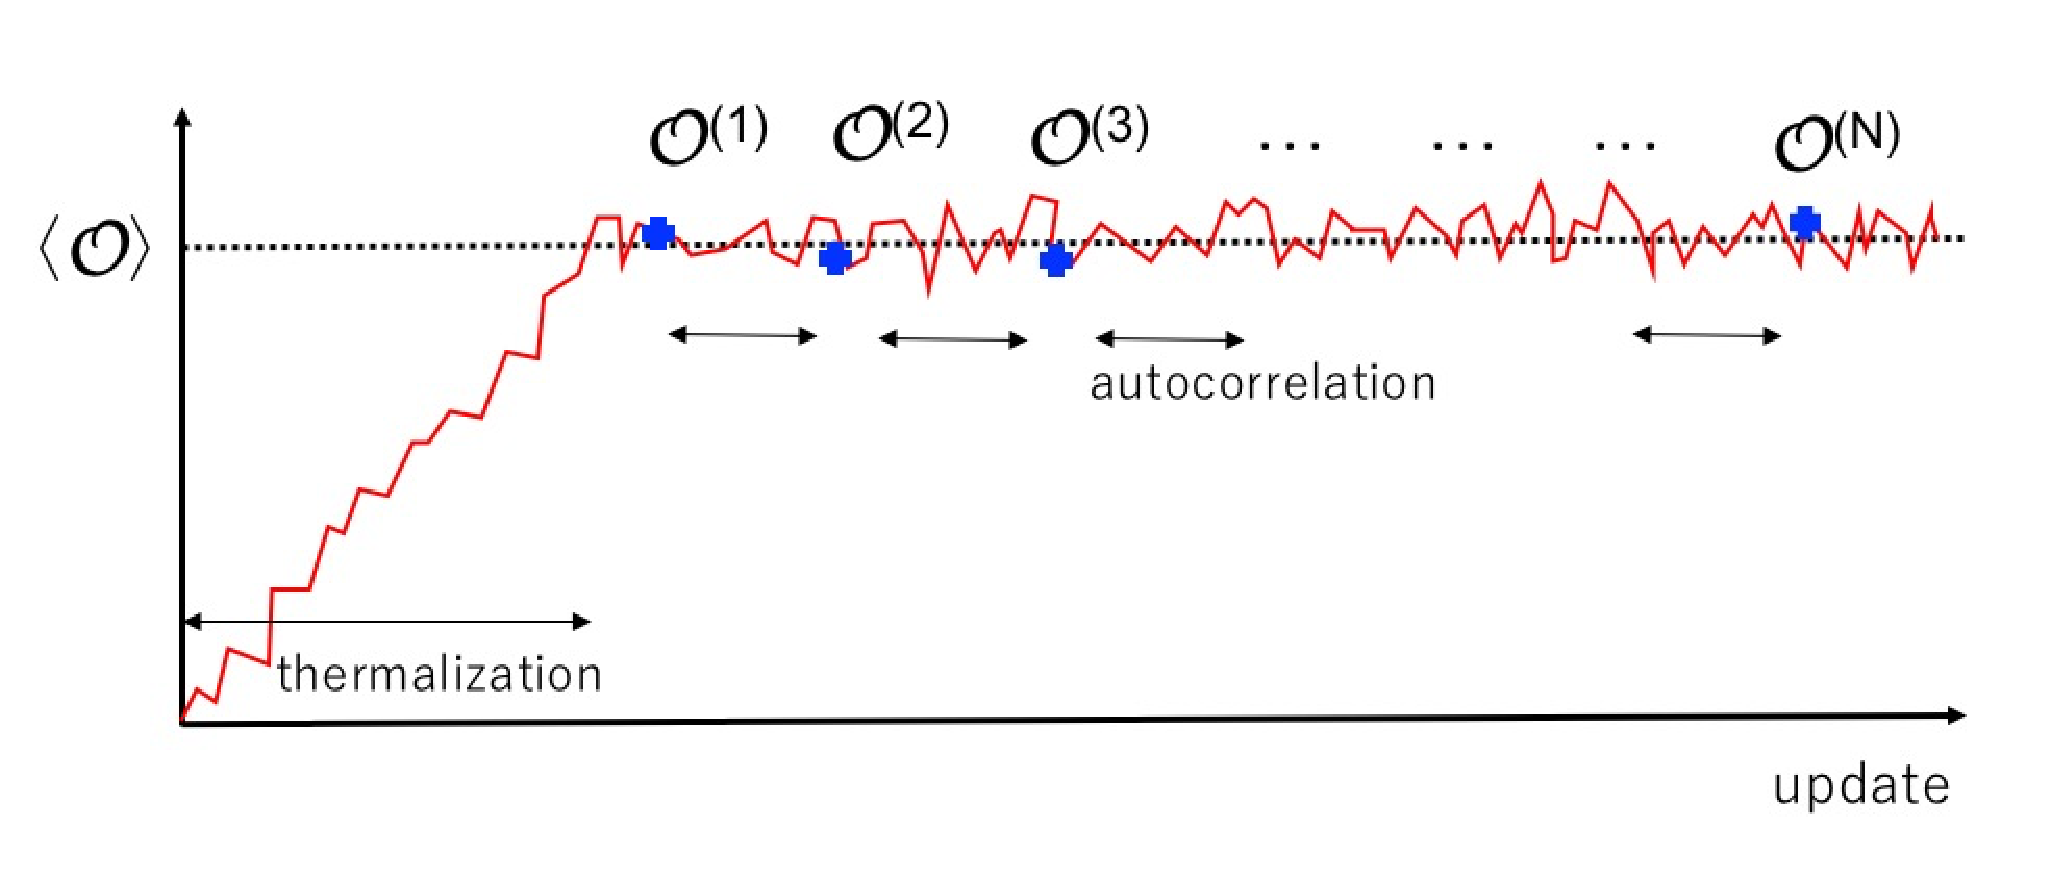
\includegraphics[scale=0.37]{Chapter3-figures/auto.eps} 
 \end{center}
\caption{Schematic illustration on the behavior of ${\cal O}$ under successive update starting from
certain initial configuration. Blue crosses correspond to ${\cal O}^{(n)}$ to be used for the actual average in
Eq.(\ref{eq:5.obs-average}).}
\label{fig:auto}
\end{figure}
%%%%%%%%%%%%%%%%%%%%%%%%%%%%%%
    
    
    
%===============================
\subsection{Hybrid Monte Carlo (HMC)}
%===============================

 Most widely used method   for 
  generating configurations in LQCD 
  is  the hybrid Monte Carlo (HMC) method \cite{Duane:1987de} and its variations.
 The basic procedure of the HMC can be summarized as follows:
 First, we rewrite the partition function by introducing a conjugate momentum field $\pi$,
 so that ${\cal Z}$ is transformed to a phase space functional integral,
\beq
{\cal Z}= \int [d\phi]\ e^{-S(\phi)}= \int [d\Phi] \  e^{- H(\Phi)}, \ \  \ \ \ 
H(\Phi) = \frac{1}{2} \pi^2 + S(\phi) ,
\eeq
where $\Phi\equiv(\phi,\pi)$ and $[d\Phi]\equiv [d\phi d\pi]$.
Then we follow the steps below:
 \begin{enumerate}
 \item[1.]   Start with arbitrary chosen initial configuration, $\phi$.
 \item[2.]  Generate $\pi$ with the Gaussian distribution, 
 \beq 
 P_{\rm G}(\pi) \propto \exp(-\pi^2/2).
 \eeq
\item[3.]  Evolve $\Phi $ under transition probability $P_{\rm H}$ with the {\it reversibility condition}, 
\beq
\label{eq:reversible}
P_{\rm H}(\Phi \rightarrow \Phi') = P_{\rm H}(\Phi'_r \rightarrow \Phi_r),   \ \ \  \Phi_r \equiv (\phi,-\pi). 
\eeq
\item[4.] Accept the configuration $\Phi'$ with the probability, 
\beq 
\label{eq:MET-test}
P_{\rm A} (\Phi \rightarrow \Phi')  = {\rm min.} \{ 1, e^{-\Delta H} \} ,
\eeq
where  $\Delta H=H(\Phi')- H(\Phi)$.  This is called the {\it Metropolis test}  \cite{Metropolis_1953}.
\item[5.] If the new configuration $\Phi'$ is accepted, go to Step 2 with $\phi'$.
 Otherwise, keep the original $\phi$ and go to Step 2. 
\end{enumerate}

The above procedure satisfies the detailed balance  Eq.(\ref{eq:5.det-balance}) 
with $W_{\rm eq}[\phi]=\exp(-S(\phi))$. 
In fact, the Step 4  satisfies the detail balance in phase space (Exercise \ref{prob:10}),
\beq
\label{eq:DT-balance}
e^{-H(\Phi)} P_{\rm A} (\Phi\rightarrow \Phi') = e^{-H(\Phi')} P_{\rm A} (\Phi' \rightarrow \Phi) .
\eeq
Then, we have
\beq
e^{-S(\phi)} P (\phi \rightarrow \phi' ) 
&=& e^{-S(\phi)} \int [d\pi d\pi'] P_{\rm G}(\pi)  P_{\rm H}(\Phi \rightarrow \Phi') P_{\rm A} (\Phi \rightarrow \Phi') , \nonumber \\
&=& \int [d\pi d\pi']\ e^{-H(\Phi)}  P_{\rm H}(\Phi \rightarrow \Phi') P_{\rm A} (\Phi \rightarrow \Phi') ,\nonumber \\
&=& \int [d\pi d\pi']\ e^{-H(\Phi')}  P_{\rm H}(\Phi \rightarrow \Phi') P_{\rm A} (\Phi' \rightarrow \Phi) ,\nonumber \\
&=& \int [d\pi d\pi']\ e^{-H(\Phi')}  P_{\rm H}(\Phi'_r \rightarrow \Phi_r)  P_{\rm A} (\Phi' \rightarrow \Phi) ,\nonumber \\
&=& \int [d\pi d\pi']\ e^{-H(\Phi')}  P_{\rm H}(\Phi' \rightarrow \Phi ) P_{\rm A} (\Phi' \rightarrow \Phi) ,\nonumber \\
&=& e^{-S(\phi')} \int [d\pi d\pi'] P_{\rm G}(\pi')  P_{\rm H}(\Phi' \rightarrow \Phi)  P_{\rm A} (\Phi' \rightarrow \Phi) 
= e^{-S(\phi')}  P (\phi' \rightarrow \phi ) ,
\eeq
where we have used Eq.(\ref{eq:reversible}) to obtain the 4th line, and also used $H(\Phi)=H(\Phi_r)$ 
 to obtain the 5th line. 

Note that $P_{\rm H}$ can be chosen to be any transition probability as long as it satisfies
Eq.(\ref{eq:reversible}).  In practice, the deterministic procedure based on the Molecular Dynamics (MD) 
evolution along the  ``computer"  time $s$ is useful:
\beq
\label{eq:MD}
\frac{d}{ds} 
\left(
\begin{array}{cc}
 \phi  \\
  \pi 
\end{array}
\right)
=
\left(
\begin{array}{cc}
 0 &  1   \\
 -1  & 0   
\end{array}
\right)
\left(
\begin{array}{cc}
  {\delta H (\phi,\pi)}/{\delta \phi}   \\
  {\delta H (\phi,\pi)}/{\delta \pi}
\end{array}
\right) =
\left(
\begin{array}{cc}
 \pi  \\
  -  {\delta S (\phi)}/{\delta \phi}
\end{array}
\right) ,
\eeq
which leads to
\beq
P_{\rm H}(\Phi \rightarrow \Phi')  = \delta (\Phi' - \Phi(s)),
\eeq
 on the phase space trajectories, $\Phi = \Phi(0) \rightarrow \Phi(s)$. 
 
If we do not introduce the MD before the Metropolis test $P_{\rm A}$,
the procedure is essentially the MCMC with the Metropolis test.  It
becomes, however, very slow for non-local action such as
Eq.(\ref{eq:Seff}) where $S_{\rm G}(U)$ is local in spacetime while
${\rm Ln Det} F(U)$ is non-local.  The MD is a nice way to evolve the
whole variables on the lattice at once.  The computer time $s$ needs
to be discretized with a step size $\varepsilon$, which brings
inevitable numerical error in MD. However, the Metropolis test in Step
4 eliminates such error so that no extrapolation to $\epsilon=0$ is
required in HMC.

 There are numerical algorithms in MD to satisfy the reversibility and
 preserve the phase space area exactly for finite $\varepsilon$.  The
 {\it leapfrog integrator} is one of such algorithms widely used in
 LQCD (see Appendix [Leapfrog integrator in molecular dynamics]).
 Since this conserves the Hamiltonian with $0(\varepsilon^2$)
 accuracy, the acceptance rate in Step 4 can be kept high.


 In LQCD simulations, we need to treat the unitary matrices $U_{\mu}(n)$ as dynamical variables, i.e.
  the MD should be performed on the SU($N_c$)  group manifold.
 The appropriate choice of the conjugate momentum would be the element of the Lie algebra,
  $ P_l =  R_l^a t^a = -i  (d{U_l}/ds) U_l^{-1} $ (see Eq.(\ref{eq:LR-form})) where
  we have abbreviated the link index $n$ and site index $\mu$  as $l$ for simplicity.
 This  leads to the
  equation of motion for $U_l$,
\beq
\label{eq:EOM-U}
\frac{d U_l}{ds}= i P_l U_l .  
\eeq
The effective Hamiltonian is naturally written as 
\beq
\label{eq:EOM-H}
H= {\rm tr} \sum_{l} P_l^2 + S_{\rm eff}(U) , 
\eeq
 where ${\rm tr}$ is over color indices with the normalization given in Eq.(\ref{eq:tt}).
 Then the  time-parameter independence  $\frac{dH}{ds}=0$ leads to the equation of motion for $P_l$
 (Exercise \ref{prob:11}),
  \beq
 \label{eq:EOM-P} 
 \frac{dP_l}{ds} = - i  \sum_{i,j} t^a \left( t^a U_l \right)_{ij} \frac{\partial S_{\rm eff}(U)}{\partial (U_l)_{ij}}.
\eeq
In the actual simulations, the ${\rm ln Det}F(U) $ part of the effective action is treated by
introducing a set of bosonic variables (pseudofermions) through the identity,
\beq
{\rm Det} F = ({\rm Det} F^{-1})^{-1} = \int [d\chi^* d\chi] \ \exp \left( -\sum_{IJ} \chi^*_{I} F_{IJ}^{-1} \chi_J \right),
\eeq
where $I$ and $J$ stand for all possible internal and spacetime indices carried by $F$.    
For further details of HMC (and its variations) with pseudofermions, 
consult the recent review \cite{Schaefer:2012tq} and references therein.


%===========================
\subsection{Error estimate}
%===========================

There are two kinds of errors  in the data obtained from  LQCD simulations.\\

\noindent {\bf Systematic errors:} \\
 They are related to the lattice spacing $a$, the lattice volume $L^3$,
  and the quark masses ($m$).  During 
  the continuum extrapolation ($a\rightarrow 0$) and the thermodynamic extrapolation ($L \rightarrow \infty$) 
  under the  guidance of  the asymptotic scaling for small $a$ 
 and the finite size scaling for  large $L$, some systematic errors are brought in.
 Also,  one often needs to make extrapolation to the physical quark mass by using 
 lattice data  with heavier  quark masses. This  also brings some
 systematic errors.\\
 
 \noindent
{\bf Statistical error:} \\
It originates from the importance sampling.  A very useful procedure to estimate such error
 commonly used in LQCD is the {\it jackknife resampling method}. (The name
  originates from the ``jackknife"  which is an easy and  portable  tool  for general purposes).
  Let us consider the mean and the unbiased variance of a certain quantity $ {\cal O}$,
  \beq
   \langle {\cal O} \rangle = \frac{1}{N} \sum_{n=1}^N {\cal O}^{(n)}  \pm \sqrt{\frac{\sigma^2({\cal O} )}{N}}, \ \ \ \
   \sigma^2({\cal O}) = \left( \frac{N}{N-1} \right)  \frac{1}{N} \sum_{n=1}^N ( {\cal O}^{(n)}  - \langle {\cal O} \rangle )^2,
  \eeq
where the factor $\frac{N}{N-1}$ is called the Bessel's correction.
 The jackknife samples are obtained by
 \beq
  {\cal O}^{(n)}_J= \frac{1}{N-1} \sum_{n' \neq n}  {\cal O}^{(n')}      \ \ \ \  (n=1, \cdots, N).
 \eeq
 If we need to make a quick estimate of the 
  mean and the variance of a function $f({\cal O})$, we have
 \beq
\label{eq:jack}
 \langle f({\cal O}_J)\rangle = \frac{1}{N} \sum_{n=1}^{N} f( {\cal O}^{(n)}_J) \pm  \sqrt{\frac{\sigma_J^2(f)}{N}}, \ \ \ \ 
  \sigma_J^2(f) = (N-1) \sum_{n=1}^N ( f( {\cal O}^{(n)}_J) -  \langle f( {\cal O}_J)\rangle)^2. 
\eeq
For $f( {\cal O})={\cal O}$, we recover the original  mean and variance;
 $\langle  {\cal O}_J \rangle = \langle  {\cal O} \rangle$ and  $\sigma_J^2({\cal O})=\sigma^2({\cal O})$. (Exercise \ref{prob:12}).
One can generalize this procedure by dividing $N$ into $N_b=N/n_b$  
with the bin-size $n_b$ and create the $N_b$ jackknife samples. 
 Eq.(\ref{eq:jack})  corresponds to the case with $n_b=1$.

 
 
%===========================
\subsection{Heavy quark potential}
%===========================

 As one of the examples of the accurate  inter-quark potential obtained from LQCD simulations,
 we  show in Fig.\ref{fig:QQbar-pot}  the  
 dimensionless ${\rm Q}\bar{\rm Q}$ potential 
$[V(R)-V(R_0)]\times R_0$
 as a function of $R/R_0$ extracted from the calculation of the   
   Wilson loop in the quenched approximation.
 $R$ is a distance between the heavy quarks
  and $R_0$ is called the {\it Sommer scale}   defined by
 $  \left. R^2 \frac{dV(R)}{dR} \right|_{R=R_0}=1.65$.
 
 Simulations with different lattice couplings $6/g^2$
  correspond to different lattice spacings $a$.
 The latter can be fixed, e.g., by   
 taking a phenomenological value
  $R_0\simeq 0.5\ {\rm fm}$. 
    The lattice spacings in the physical uniit in the figure are
   $a=0.094\ {\rm fm}$ (squares: $\beta=6/g^2=6.0$),
    $a= 0.069\ {\rm fm}$ (circles: $\beta=6.2$)
  and  $a=0.051\ {\rm fm}$ (triangles: $\beta=6.4$).
  Since there exists no appreciable $a$ dependence of the potential,
 the system is already close enough to the continuum limit. 
  
 Fig.\ref{fig:QQbar-pot} clearly shows that the 
  heavy quark potential has a linear confining part
   at long distance and an attractive Coulombic part 
    at short distance. The LQCD results agree
     not only qualitatively but also quantitatively  
  with an empirical linear + Coulomb potential
  (the Cornell potential)    shown by the solid line,
   $V(r) = Kr - b/r + {\rm const}$ with $b=0.295$.  
   
% FIG %%%%%%%%%%%%%%%%%%%%%%%%%%   
\begin{figure}[t]
\begin{center}
%\framebox[74mm]{\rule[-26mm]{0mm}{52mm}}
%\includegraphics[scale=0.6]{as-scale.eps}
\includegraphics[scale=0.5]{Chapter3-figures/QQbar-pot.eps} 
 \end{center}
\caption{A dimensionless ${\rm Q}\bar{\rm Q}$ potential as a 
 function of a dimensionless quark$-$anti-quark
 separation $R/R_0$ with $R_0$ being the Sommer scale. 
 Different  symbols correspond to different lattice couplings
  $g(a)$    and hence different lattice spacings. 
  The solid line shows an empirical Cornell potential. 
  The figure is adapted from \cite{Bali:2000gf}.
  }
\label{fig:QQbar-pot}
\end{figure}
%%%%%%%%%%%%%%%%%%%%%%%%%%%%%%


%============================
\subsection{Masses of light hadrons}
%============================

 Meson masses and baryon masses can be calculated with high accuracy
 by LQCD simulations with dynamical quarks.  The starting point is the
 hadronic correlation functions $C_{\rm H=M,B} (n,n')$ in
 Eqs.(\ref{eq:correlation-M},\ref{eq:correlation-B}) integrated over
 the spatial coordinates, $\mathbf{n}$ and
 $\mathbf{n}'$, 
\beq \label{eq:5.D-tau} C_{\rm H}(\tau)
 = \sum_{\mathbf{n}, \mathbf{n}'} C_{\rm H}
 (n,n') \xrightarrow[\tau \rightarrow \infty] \ |Z_{\rm H}|^2 {\rm
 e}^{-M_{\rm H} \tau} , 
\eeq 
where $\tau= (n_4-n_4')a$ is the temporal
 distance between the source at $n'$ and the sink at $n$, and $M_{\rm
 H}$ ($Z_{\rm H}$) corresponds to the mass (the pole residue) of a
 lightest bound state in each channel.  If the temporal extent of the
 lattice is infinite, one can extract the hadron mass from the
 formula, $M_{\rm H}= -(1/\tau) \ln C_{\rm
 H}(\tau)|_{\tau \rightarrow \infty} $.  In practice, the {\it
 effective mass} defined below is more useful, \beq aM_{\rm H}^{\rm
 eff}(\tau) = \ln \left( \frac{C_{\rm H}(\tau)}{C_{\rm H}(\tau+a)
 } \right) .
\eeq
The asymptotic plateau of the effective mass at large $\tau$
     corresponds to the hadron mass.  In actual simulations, the
     temporal extent is limited ($0 \le \tau/a \le N_{\tau}$), so that
     the exponential damping of Eq.(\ref{eq:5.D-tau}) is replaced by
     $C_{\rm H} \rightarrow \exp[-M_{\rm H} \tau ] \pm \exp [-M_{\rm
     H} (N_{\tau} a - \tau)]$ where $+ (-)$ for the periodic
     (anti-periodic) boundary condition.
     
 Shown in the left panel of Fig.\ref{fig:hadron-mass} is the
 dimensionless effective masses ($a M_{\rm H}^{\rm eff}$) against
 $\tau/a=(n_4-n_4')$ \cite{Durr:2008zz}.  Data points are the
 effective masses for the pion $(\pi)$, the kaon $(K)$, the nucleon
 ($N$), the cascade baryon ($\Xi$) and the omega baryon $(\Omega$)
 calculated on the lattice with $a \simeq 0.085$ fm and the pion mass
 $M_{\pi} \simeq 190$ MeV.  Reasonable plateau above $\tau/a > 9$ can
 be seen within the error bars.
 
 Shown in the right panel of Fig.\ref{fig:hadron-mass} is the
 $M_{\pi}^2$-dependence of the $N$ and $\Omega$ masses for three
 different values of $a$ \cite{Durr:2008zz}.  The crosses are the
 values extrapolated to the continuum limit and to the physical pion
 mass.  The $N$ and $\Omega$ masses predicted from LQCD and
 corresponding experimental numbers are
\beq
\label{eq:mass-LQCD}
M_N^{\rm LQCD} &=& 0.936(25)(22) \ {\rm GeV}, \ \ \ M_\Omega^{\rm
LQCD} =1.676(20)(15)\ {\rm GeV}, \\ M_N^{\rm exp.} &=& 0.939 \ {\rm
GeV}, \ \ \ \ \ \ \ \ \ \ \ \ \ \ \ \ M_\Omega^{\rm exp.} =1.672 \
{\rm GeV}.
\eeq
  Note that the numbers in the first (second) parenthesis in
 Eq.(\ref{eq:mass-LQCD}) represent the statistical (systematic) errors
 on the last digits.

% FIG %%%%%%%%%%%%%%%%%%%%%%%%%%   
\begin{figure}[t]
\begin{center}
%\framebox[74mm]{\rule[-26mm]{0mm}{52mm}}
%\includegraphics[scale=0.6]{as-scale.eps}
\includegraphics[scale=0.29]{Chapter3-figures/effective-mass.eps} \ \ 
\includegraphics[scale=0.28]{Chapter3-figures/NO_scaling.eps}
 \end{center}
\caption{(Left) The effective masses of hadrons against the 
 temporal separation between the source and the sink. 
(Right)  Hadron masses under the changes of the (pion mass)$^2$ as well as the lattice spacing $a$.
The figures are taken from \cite{Durr:2008zz}
  }
\label{fig:hadron-mass}
\end{figure}
%%%%%%%%%%%%%%%%%%%%%%%%%%%%%%%

Shown in Fig.\ref{fig:pn-mass} are the high precision numerical
 results of the hadron mass splittings obtained by the QCD+QED lattice
 simulations with dynamical $u,d,s,c$ quarks \cite{Borsanyi:2014jba}.
 The horizontal lines are the experimental values and the grey shaded
 regions represent the experimental errors.  Red dots are the lattice
 results with their uncertainties denoted by the vertical error bars.
 The neutron-proton mass differences from numerical simulations and
 the corresponding experimental numbers are
\beq
(M_n-M_p)^{\rm LQCD+QED} &=&\Delta N = 1.51(16)(23)\   {\rm MeV}, \\
(M_n-M_p)^{\rm exp.} &=& 1.29\   {\rm MeV}. 
\eeq

% FIG %%%%%%%%%%%%%%%%%%%%%%%%%%
\begin{figure}[t]
\begin{center}
%\framebox[74mm]{\rule[-26mm]{0mm}{52mm}}
%\includegraphics[scale=0.6]{as-scale.eps}
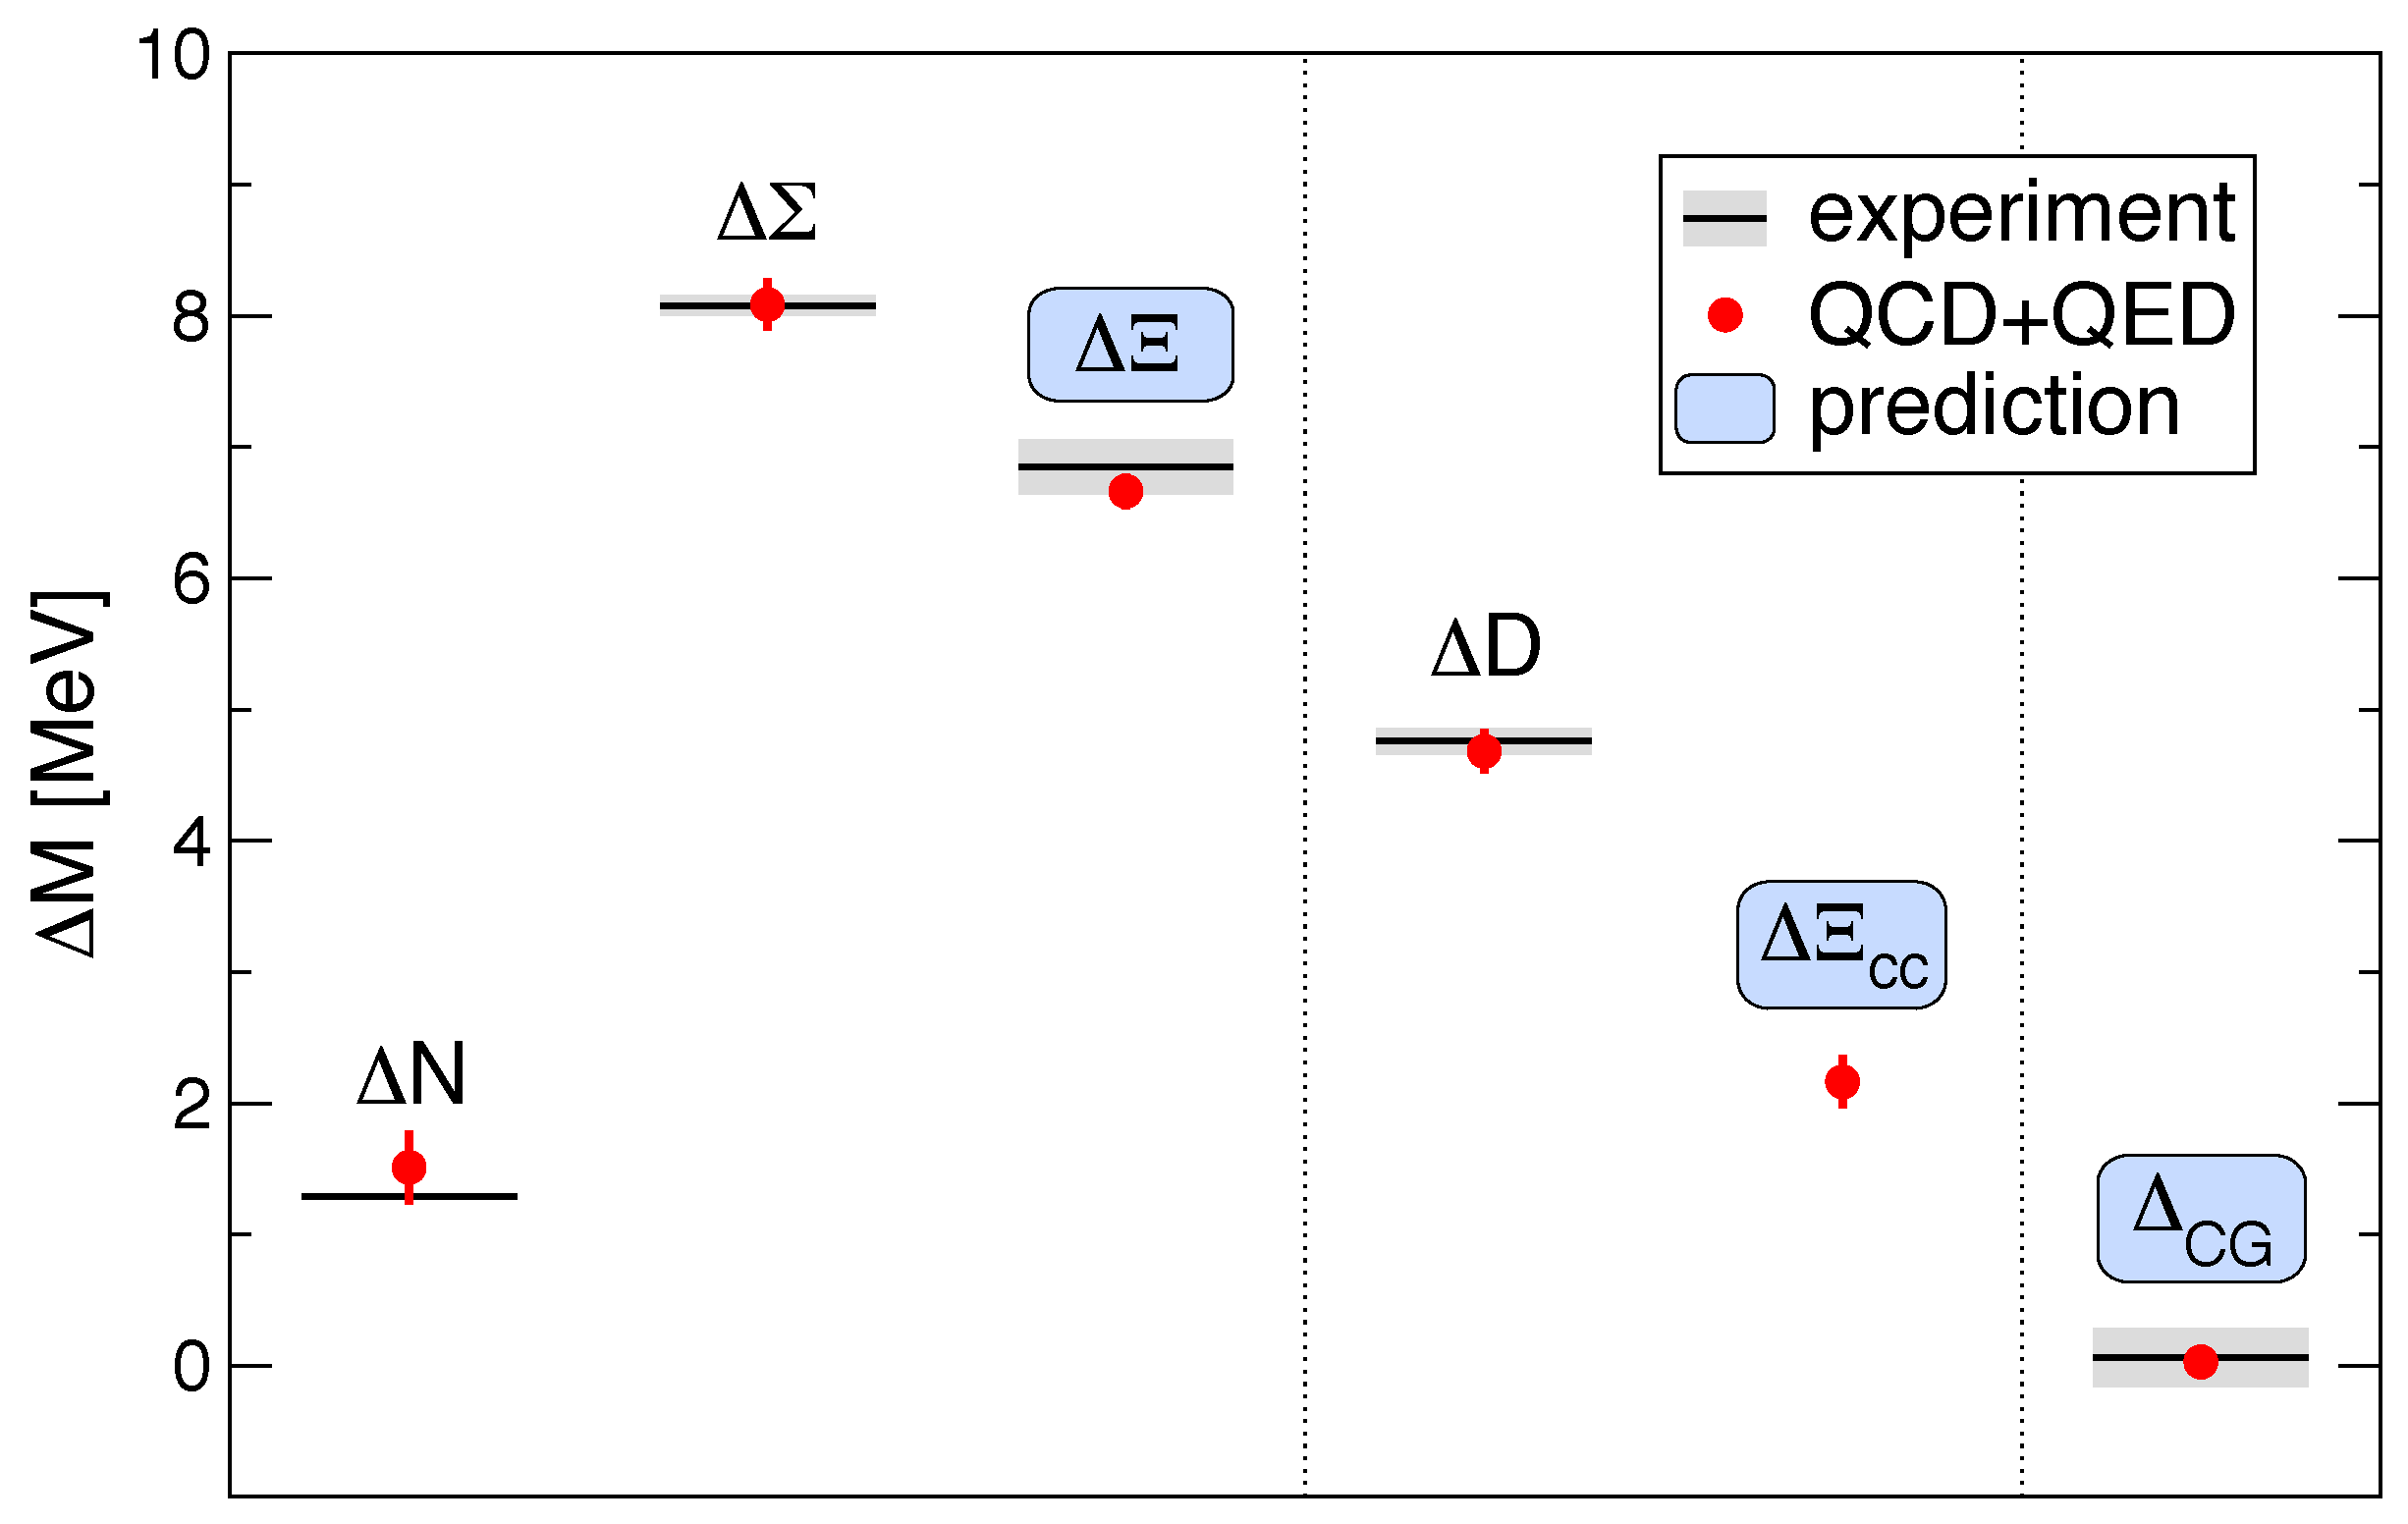
\includegraphics[scale=0.2]{Chapter3-figures/pn-mass.eps}
 \end{center}
\caption{Mass splittings in channels that are stable under the strong and electromagnetic interactions.
$\Delta N=M_n-M_p$, $\Delta \Sigma = M_{\Sigma^-}- M_{\Sigma^+}$,
$\Delta \Xi =M_{\Xi^-}- M_{\Xi^+}$,
$\Delta D= M_{D^{\pm}} - M_{D^0}$,
$\Delta \Xi_{cc} = \Delta \Xi_{cc}^{++} - \Delta \Xi_{cc}^{+}$,
$\Delta CG = \Delta N-\Delta \Sigma + \Delta \Xi$.
The figure is taken from
\cite{Borsanyi:2014jba}.
  }
\label{fig:pn-mass}
\end{figure}
%%%%%%%%%%%%%%%%%%%%%%%%%%%

Since all hadrons are composite particles of quarks and gluons, there
are numerous excited states \cite{RPP}.  To extract the properties of
the excited hadrons from LQCD, only looking at the asymptotic form as
shown in Eq.(\ref{eq:5.D-tau}) is not sufficient, and more
sophisticated methods such as the maximal entropy method (MEM) and the
variational method are required.  Interested readers should consult
the reviews \cite{Asakawa:2000tr,Fodor:2012gf} and references there
in.


%%%%%%%%%%%%%%%%%%%%%%%%
\section{Lattice QCD and nuclear force}
%%%%%%%%%%%%%%%%%%%%%%%%

Understanding of the nuclear force from QCD is one of the most
 challenging problems in nuclear physics.  Below the pion production
 threshold, the notion of the $NN$ potential (either in the coordinate
 space or in the momentum space) has been known to be useful, since it
 can be used not only to describe the two-body system but also to
 study nuclear many-body problems through ab-initio
 calculations \cite{this_book}.

  Several high precision phenomenological $NN$ forces have been
  constructed to reproduce the neutron-proton and proton-proton
  scattering data (about 4500 data points) with a $\chi^2/{\rm
  dof} \sim 1$. However, they have typically 20-40 fitting parameters:
  e.g. the CD Bonn potential, AV18 potential and N$^3$LO chiral
  effective field theory have 38, 40, and 24 parameters,
  respectively \cite{Machleidt:2007ms}.  If one tries to extend these
  to hyperon-nucleon and hyperon-hyperon interactions, the task
  becomes extremely tough since the number of parameters increases and
  the scattering data are scarce.
 
  Under this situation, it is highly desirable to study
  baryon-baryon interactions from first principle LQCD simulations,
  where all the hadronic interactions are controlled only by the QCD
  coupling $g$ and the quark mass $m$ whose values are pretty well
  determined at present by the precision QCD
  simulations \cite{Aoki:2013ldr}.
 
 The finite volume method (FVM), a theoretical framework to study
  hadron-hadron interactions from LQCD, was first proposed by
  L\"{u}scher \cite{luescher}: For two hadrons in a finite box with a
  spatial size $L^3$, an exact relation between the energy spectra in
  the box and the elastic scattering phase shift can be derived.  If
  the range of the hadronic interaction $R_{\rm QCD}$ is sufficiently
  smaller than the size of the box $R_{\rm QCD}<L/2$, the behavior of
  the the equal-time Bethe-Salpeter amplitude (or more precisely the
  Nambu-Bethe-Salpeter (NBS) amplitude) $\psi (\mathbf{r})$ in the
  interval $R_{\rm QCD} < | \mathbf{r} | < L/2 $ has sufficient
  information to relate the phase shift and the energy shift 
$\Delta E=M_{\rm HH}-2M_{\rm H}$.
  
The HAL QCD method was proposed as another theoretical framework to
 study the hadron-hadron interactions from LQCD by Ishii, Aoki and
 Hatsuda \cite{Ishii:2006ec} and was further developed by HAL QCD
 Collaboration \cite{HALQCD:2012aa}.  The starting point is the same
 equal-time NBS amplitude $\psi (\mathbf{r})$: Instead of looking at
 the amplitude outside the range of the interaction, the internal
 region $ |\mathbf{r} | < R_{\rm QCD}$ is considered and an
 energy-independent non-local potential $U(\mathbf{r}, \mathbf{r}')$
 is deduced from $\psi (\mathbf{r})$.  Since
 $U(\mathbf{r}, \mathbf{r}')$ in QCD is spatially localized due to the
 confinement of quarks and gluons, it is affected only weakly by the
 finite lattice volume. Physical quantities such as the scattering
 phase shifts, bound state spectra, and resonance energies can be
 calculated by solving the integro-differential differential equation
 satisfied by $\psi (\mathbf{r})$ with $U(\mathbf{r}, \mathbf{r}')$.
   
  Recently, a detailed comparison between the FVM and the HAL QCD
  method has been carried out: Although they agree with each other
  quite accurately for non-resonant pion-pion scattering, large signal
  to noise ratio inherent in the effective mass $\Delta E^{\rm
  eff}(\tau)$ for baryon-baryon scatterings prevents FVM to extract
  scattering observables \cite{Iritani:2015dhu}.  Therefore, we will
  focus on the HAL QCD method below.
  
%=============================================     
\subsection{Master equation for baryon-baryon interaction}
%=============================================  
  
Let us consider the baryon-baryon correlation in
Fig.\ref{fig:correlation}(c) and define the equal-time NBS amplitude
$\psi_{\ell}(\mathbf{r},\tau)$ from its large $\tau$ behavior: 
\beq
C_{\rm BB}(\mathbf{r}, \tau)
=\sum_{\mathbf{n}',\mathbf{m}'} \left. C_{\rm
BB}(n,m,n',m') \right|_{n_4=m_4,n_4'=m_4'} \rightarrow \sum_{\ell}
a_{\ell} \psi_{\ell} (\mathbf{r},\tau) e^{-E_{\ell} \tau} , 
\eeq 
where
$\mathbf{r}=(\mathbf{n}-\mathbf{m}) a$, $\tau=(n_4-n_4')a$, and
$\psi_{\ell} (\mathbf{r},\tau)$ being the NBS wave function for
$\ell$-th scattering state on the lattice.  For large lattice size,
$E_{\ell}$ is very dense, so that it is impossible to identify each
level.  This causes a fatal problem in FVM as mentioned above.  On the
other hand, if we define $ C_{\rm BB}(\mathbf{r};\tau)= {\cal
R}(\mathbf{r},\tau) e^{-2M_{\rm B} \tau}$, the following
integro-differential equation can be derived below the inelastic
threshold ($\tau > M_{\pi}^{-1}$),
\beq
  \left\{
  \frac1{4M_{\rm B}}\frac{\partial^2}{\partial \tau^2} 
  -\frac{\partial}{\partial \tau}
  - H_0
  \right\}
  {\cal R}(\mathbf{r},\tau)
  =
  \int d^3 r'
  U(\mathbf{r}, \mathbf{r}')
  {\cal R}(\mathbf{r}', \tau),
  \label{eq.tdep}
\eeq
 with  $H_0= - \nabla^2/M_{\rm B}$.
 This is the master equation which has the 
correct information of the S-matrix and hence the scattering phase shift for
elastic $BB$ scatterings \cite{HALQCD:2012aa}.
  
  If we further focus on the 
  energies  much below  the inelastic threshold,
   the velocity expansion
   of $U(\mathbf{r},\mathbf{r}')$ in terms of its  non-locality can be adopted.
   In fact, the potential with hermiticity, 
   rotational invariance, parity symmetry,   and time-reversal invariance may be expanded as \cite{okubo}
\begin{eqnarray} 
\label{eq:U-del}
  U(\mathbf{r},\mathbf{r}')    &=& V(\mathbf{r}, \mathbf{v}) \delta(\mathbf{r}-\mathbf{r}'), \\
 V(\mathbf{r}, \mathbf{v})    & =&
   \underbrace{V_{\rm C}(r) + V_{\rm T}(r) S_{12}}_{\rm LO} 
  + \underbrace{V_{\rm LS}(r) {\mathbf{L}} \cdot {\mathbf{S}}}_{\rm NLO}  
  +\underbrace{{O}(\mathbf{v}^2)}_{{\rm N}^2{\rm LO}}
  + \cdots , 
   \label{eq:V-pot}
\end{eqnarray} 
   where $\mathbf{v} = \mathbf{p}/(M_{\rm B}/2) $, $\mathbf{L} = \mathbf{r} \times \mathbf{p} $, 
   $\mathbf{p} = -i \nabla$ and 
   $S_{12}=3(\mathbf{\sigma}_1 \cdot \mathbf{r})(\mathbf{\sigma}_2 \cdot \mathbf{r})/r^2 - \mathbf{\sigma}_1 \cdot \mathbf{\sigma}_2$.
     The central potential $V_{\rm C}$ and 
  the tensor potential $V_{\rm T}$ are classified as
  the leading order (LO) potentials since they
  are of $O(\mathbf{v}^0)$. The next-to-leading (NLO) potential of  
  $O(\mathbf{v})$ is the spin-orbit potential  $V_{\rm LS}(r)$. 

%=============================================
\subsection{Baryon-baryon interaction in flavor SU(3) limit}
%=============================================  
  
 % FIG %%%%%%%%%%%%%%%%%%%%%%%%%%
\begin{figure}[t]
\begin{center}
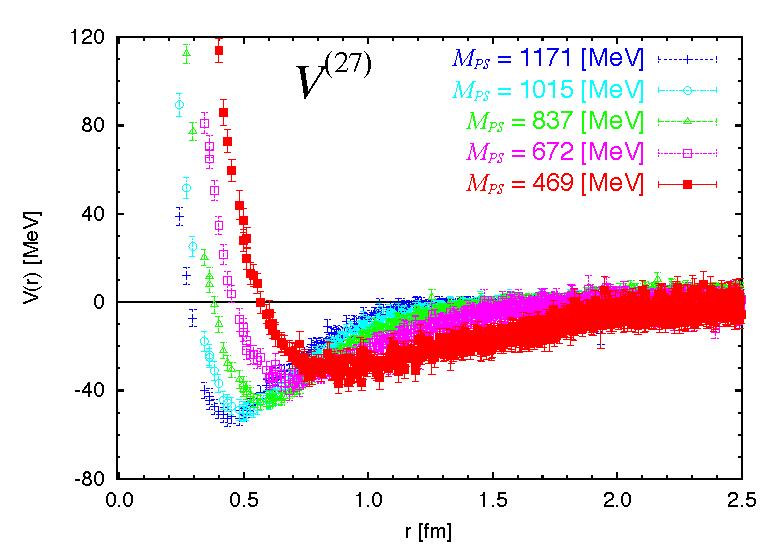
\includegraphics[scale=0.55]{Chapter3-figures/Vc_27_npa2.eps}\ \ \ \ \ \ \ 
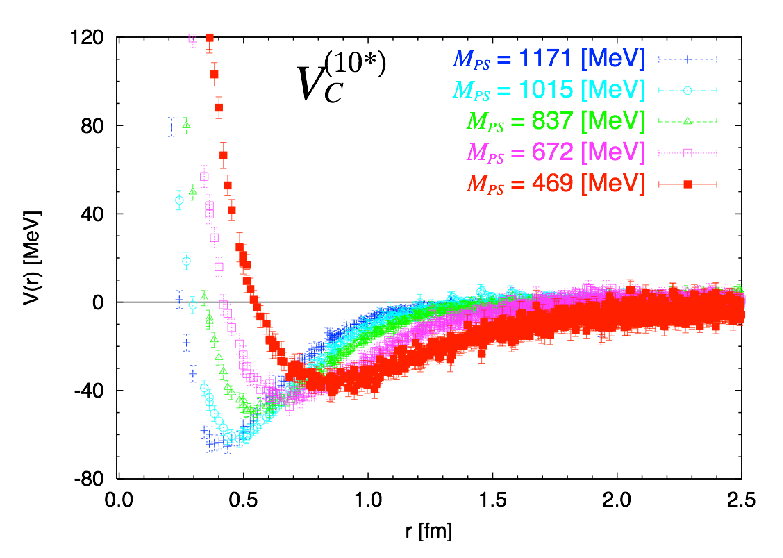
\includegraphics[scale=0.55]{Chapter3-figures/Vc_10s_npa2.eps}\\
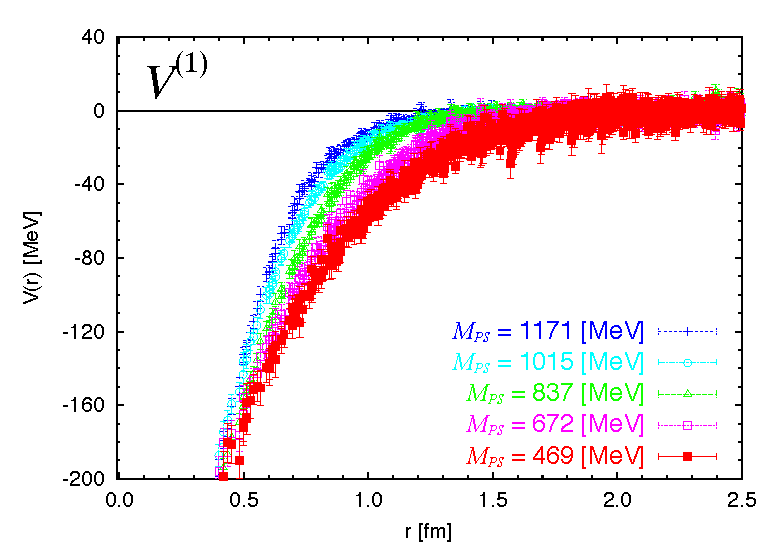
\includegraphics[scale=0.55]{Chapter3-figures/Vc_1_npa2.eps}\ \ \ \ \ \ \ 
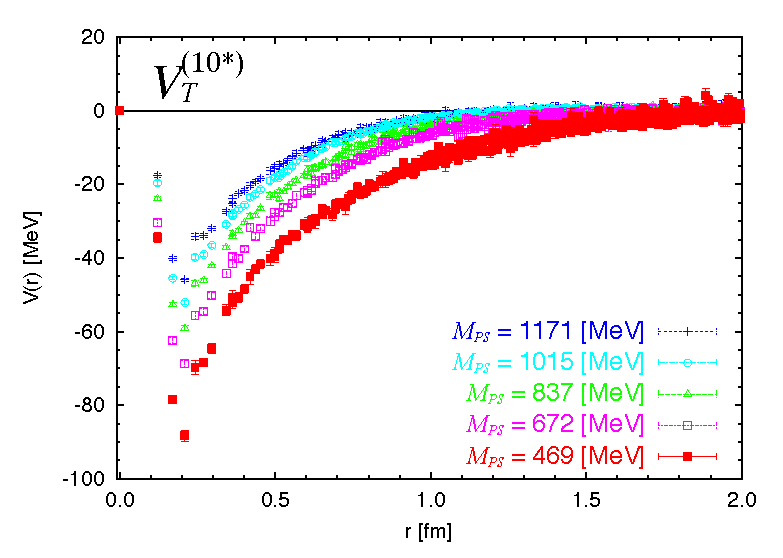
\includegraphics[scale=0.55]{Chapter3-figures/Vt_10s_npa2.eps}
 \end{center}
\caption{The baryon-baryon potentials from LQCD simulations in the flavour
SU(3) limit with several different masses of pseudo-scalar meson. 
The figures are taken from \cite{Inoue:2011ai}.
  }
\label{fig:NN-potential}
\end{figure}
%%%%%%%%%%%%%%%%%%%%%%%%%%%%%
  
 To obtain qualitative understandings of the nuclear force from QCD,
  the $S$-wave interaction between octet baryons  
 in the flavour SU(3) limit  would be a good starting point.
 In this case,  two baryon states with a given angular momentum
are labelled by the irreducible flavour multiplets,
\begin{equation}
 {\bf 8} \otimes {\bf 8} 
 = \underbrace{{\bf 27} \oplus {\bf 8}_s \oplus {\bf 1}}_{\mbox{symmetric}} ~ 
  \oplus \underbrace{{\bf 10}^* \oplus {\bf 10} \oplus {\bf 8}_a}_{\mbox{anti-symmetric}} \ . 
\end{equation}
Here ``symmetric" and ``anti-symmetric" stand for the symmetry under the
flavour exchange of two baryons.
For the system in the orbital S-wave, the Pauli principle between two baryons imposes 
${\bf 27}$, ${\bf 8}_s$ and ${\bf 1}$ to be spin singlet  ($^1S_0$) while 
${\bf 10}^*$, ${\bf 10}$ and ${\bf 8}_a$ to be spin triplet ($^3S_1$). 
Since there are no mixings among different multiplets in the SU(3) limit, 
one may define the corresponding potentials as
 \beq
^1S_0 \ &:& \  V^{({\bf 27})}(r), \ V^{({\bf 8}_s)}(r), \ V^{({\bf 1})}(r), 
\\ 
^3S_1 \ &:& \ V^{({\bf 10}^*)}(r), \ V^{({\bf 10})}(r), \ V^{({\bf 8}_a)}(r) ~.
\eeq
The diagonal potential ($B_1B_2 \rightarrow B_1 B_2)$ and  
 the off-diagonal potentials ($B_1B_2 \rightarrow B_3 B_4$) in the particle basis, 
 are obtained by  suitable combinations
of $V^{(\alpha)}(r)$ with $\alpha={\bf 27},{\bf 8}_s,{\bf 1},{\bf10}^*,{\bf 10},{\bf 8}_a$.

% FIG %%%%%%%%%%%%%%%%%%%%%%%%%%
\begin{figure}[t]
\begin{center}
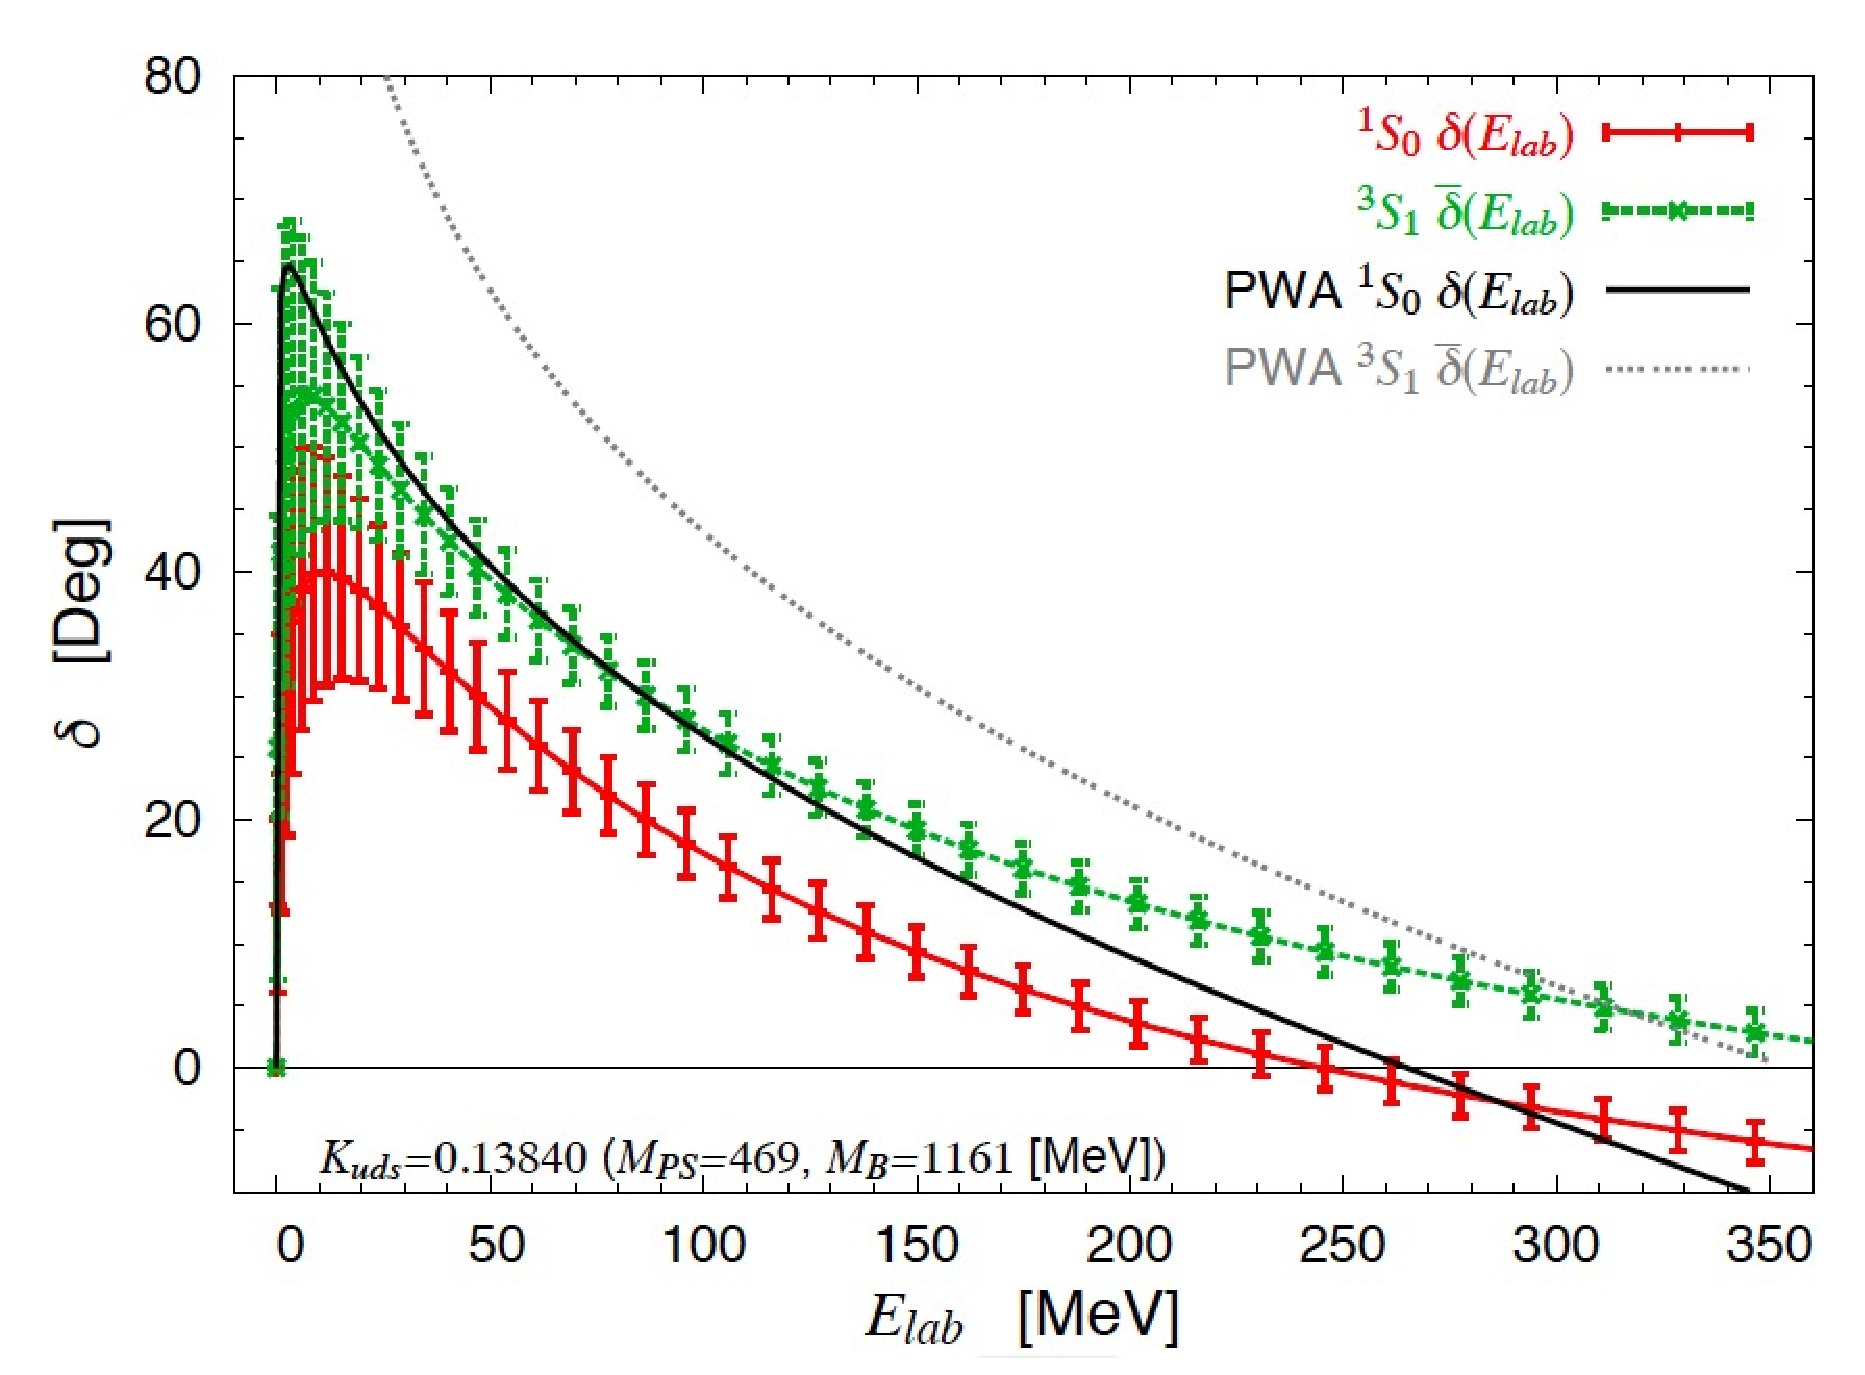
\includegraphics[scale=0.25]{Chapter3-figures/phase-shift.eps}\ \ \ \ 
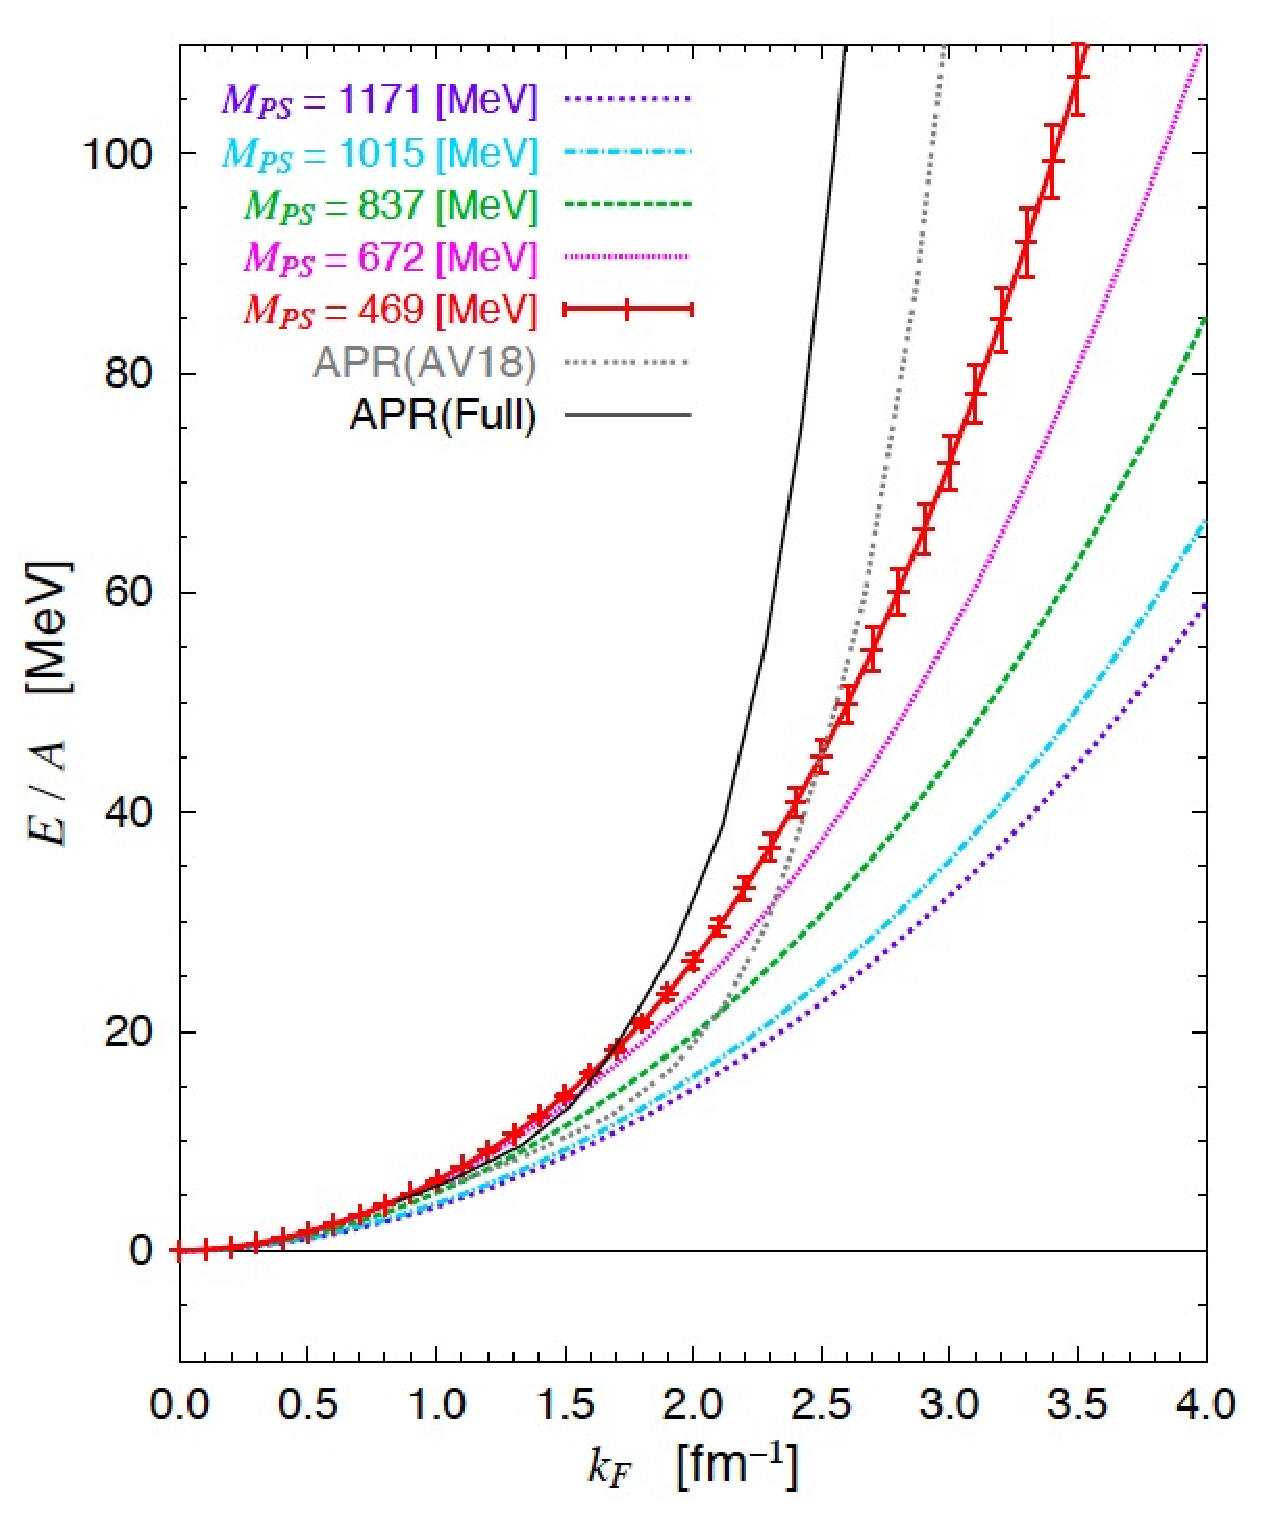
\includegraphics[scale=0.27]{Chapter3-figures/neutron-matter.eps}
 \end{center}
\caption{(Left) Phase shifts of the NN scattering as a
function of energy in the laboratory frame, extracted from
LQCD data at the pion mass 469 MeV in the flavor-SU(3) limit.
 The black and gray dashed lines are the results of the partial wave
analysis (PWA) of the experimental data. (Right) Ground state energy per neutron for the
pure neutron matter as a function of the Fermi momentum.
 The APR with black dotted line (black solid line)   corresponds to the empirical equation of state without (with) the
phenomenological three nucleon force \cite{Akmal:1998cf}.
 \cite{Akmal:1998cf}.
The figures are taken from \cite{Inoue:2013nfe}.
  }
\label{fig:NN-phase_shift}
\end{figure}
%%%%%%%%%%%%%%%%%%%%%%%%%%%%%%


Shown in Fig.\ref{fig:NN-potential}  are the results of the exploratory study of the potentials
obtained by LQCD simulations on the lattice  with $a\simeq 0.12$ fm, 
$L\simeq 4$ fm and 3 degenerate flavours  \cite{Inoue:2011ai}.  Corresponding pion mass ranges from
 469 MeV to 1171 MeV. 
\begin{itemize}
\item  The upper left panel is the 
central potential $V^{({\bf 27})}(r)$ to which the  $^1S_0$ nucleon-nucleon potential belongs.
 It  has a repulsive core at short distance and an attractive pocket at intermediate distance.
As the pion mass decreases,  the repulsive core gets stronger and the attractive tail gets
 longer.  
\item As shown in the lower left panel, the structure of the potential is quite different for $V^{({\bf 1})}(r)$ to which the
  flavour singlet $H$ dibaryon (composed of $uuddss$) belongs.   There is no repulsive core and the attraction 
  increases as the pion mass decreases.  Such a feature is consistent with the 
   notion of  the quark Pauli principle previous discussed in phenomenological quark models \cite{Oka-Fujiwara}.
\item The upper and lower right panels of  Fig.\ref{fig:NN-potential}  are the 
central potential and the tensor potential of $V^{({\bf 10}^*)}(r)$, respectively. The
$^3S_1$ nucleon-nucleon potential belongs to this channel. The central part has a similar
structure as the $^1S_0$ channel, while the tensor part has strong attraction and grows rapidly  as the 
 pin mass decreases.  The latter aspect is qualitatively consistent with the one-pion-exchange picture at
 long distances.
 \end{itemize}
   
 Shown in  Fig.\ref{fig:NN-phase_shift} (left) is  the nucleon-nucleon scattering phase shifts
  in the $^1S_0$ channel and $^3S_1$ channel obtained by using the 
   potentials, $V^{({\bf 27})}(r)$ and $V^{({\bf 10}^*)}(r)$,  for the pion mass 469 MeV \cite{Inoue:2013nfe}.
   The qualitative feature of the 
   phase shift in the $^1S_0$ channel is similar to the experimental one denoted by the 
   black solid  line, despite the fact that pion mass in the simulation is  more than 3 times
   heavier than the physical value. In the  $^3S_1$ channel, the deuteron bound state is 
   not formed yet due to heavy pion mass, so that the phase shift starts from 0 at zero energy
    in contrast the the experimental one denoted by the black dashed line.
    There is however a tendency that the attraction in the $^3S_1$ channel is larger than
   the $^1S_0$ channel even for the heavy pion mass.
  Shown in  Fig.\ref{fig:NN-phase_shift} (right) is  the energy per particle $E/A$ as a function of the 
  fermi momentum $k_{\rm F}$ for pure neutron matter calculated by using the Brueckner-Hartree-Fock method
  with the neutron-neutron potential in the $^1S_0$ channel in Fig.\ref{fig:NN-phase_shift} (left). 
 As the pion mass decreases, the equation of state becomes stiffer due to the growth of the repulsive  core. 
 The APR with black dotted line (black solid line)   corresponds to the empirical equation of state without (with) the
phenomenological three nucleon force  \cite{Akmal:1998cf}.

 We note that calculations of the baryon-baryon interactions  with  
  (2+1)-flavour LQCD on a large volume ($L \simeq 8.2 {\rm fm}$, $a\simeq 0.085$ fm) at
   nearly the physical quark mass ($m_{\pi}\simeq146$ MeV, $m_{K}\simeq$ 525 MeV)
   are underway  \cite{Doi:2015oha}.
 
  
%%%%%%%%%%%%%
\section{Exercises}
%%%%%%%%%%%%%

\begin{prob} \label{prob:1}
Prove the properties of the Wilson line, Eqs.(\ref{eq:5.wilson-line-i}), (\ref{eq:5.wilson-line-ii}), and (\ref{eq:5.wilson-line-iii}).
\end{prob}

\begin{prob}\label{prob:2}
Derive the expression on $U_{\mu \nu}(n)-1$ in 
Eq.(\ref{eq:5.wilson-plaq-cont-2}) by using the Baker-Campbell-Hausdorff formula.
\end{prob}

\begin{prob}\label{prob:3}
Show the $\Gamma_5$ Hermiticity of the Dirac operator in Eq.(\ref{eq:gamma5-hermite}).
\end{prob}

\begin{prob}\label{prob:4}
Derive  the free fermion propagator on the lattice in the momentum representation,
Eqs.(\ref{eq:DF}) and (\ref{eq:Mp}). 
\end{prob}

\begin{prob}\label{prob:5}
Analyze the dispersion relation of the free fermion associated with the 
Dirac operator, $D_{\rm GW}$ in Eq.(\ref{eq:5.overlap-op}).
\end{prob}

\begin{prob}\label{prob:6}
Derive the group integration formulas, Eq.(\ref{eq:group-int-1})- Eq.(\ref{eq:group-int-B}), by taking appropriate 
contractions of the color indices.
\end{prob}


\begin{prob}\label{prob:7}
Derive the formula for the Wilson loop in the strong coupling limit Eq.(\ref{eq:5.wilson-strong}) by using the group integration formulas
Eqs.(\ref{eq:group-int-0})-(\ref{eq:group-int-2}). 
\end{prob}

\begin{prob}\label{prob:8}
Derive the lattice coupling $g(a)$ as a function of the lattice spacing $a$, Eq.(\ref{eq:5.lat-running-g}).
\end{prob}

\begin{prob}\label{prob:9}
Show the convergence of $W[\phi]$ to the equilibrium distribution $W_{\rm eq}[\phi]$
under the Markov process by introducing the distance $D= \sum_{\phi} \left| W[\phi] -W_{\rm eq}[\phi] \right| $
 and by studying its behavior under update.
\end{prob}

\begin{prob}\label{prob:10}
Prove that the Metropolis test in Eq.(\ref{eq:MET-test})
satisfies the detailed balance Eq.(\ref{eq:DT-balance}).
\end{prob}

\begin{prob}\label{prob:11}
Derive the equation of motion for $P_l$ in Eq.(\ref{eq:EOM-P})
from Eq.(\ref{eq:EOM-U}) and  Eq.(\ref{eq:EOM-H}).
\end{prob}

\begin{prob}\label{prob:12}
Prove that the jackknife average and variance for $f({\cal O})={\cal O}$ reduce to the 
standard mean and unbiased variance, respectively.
\end{prob}

\begin{prob}\label{prob:13}
Prove that  the leapfrog integrator satisfies the reversibility Eq.(\ref{eq:reversible}) exactly.
Also prove that  the leapfrog integrator preserves the phase space area exactly by
evaluate the Jacobian, $d\phi' d\pi'= J d\phi d\pi $. 
\end{prob}
 

%%%%%%%%%%%%%%%%
\begin{acknowledgement}
%%%%%%%%%%%%%%%%
%If you want to include acknowledgments of assistance and the like at the end of an individual chapter 
%please use the \verb|acknowledgement| environment -- it will automatically render Springer's preferred layout.
The author thanks Takumi Doi and Atsushi Nakamura for useful comments and information on various aspects of
LQCD simulations.
He also thank the members of HAL QCD Collaboration for  fruitful discussions on the hadron-hadron interactions 
on the lattice.
This work was supported in part by MEXT SPIRE and JICFuS and also by RIKEN iTHES Project.
\end{acknowledgement}
%

\section{Appendix}
\addcontentsline{toc}{section}{Appendix}

%%%%%%%%%%%%%%%%%%%%%%%%%%%%
\subsubsection*{\center{Four vectors and Dirac matrices}}
%%%%%%%%%%%%%%%%%%%%%%%%%%%%

In the (3+1)-dimensional  Minkowski spacetime, coordinates, derivatives 
and four vectors with $\mu=0,1,2,3$ are
\beq
x^{\mu} = (t, \mathbf{x}),
\ \ \partial^{\mu}   =  (\partial_t, -\nabla),
\ \  A^{\mu} =(A^0, \mathbf{A}).
\label{eq:B.vector-M}
\eeq
In the 4-dimensional Euclidean space, 
 we define the corresponding vectors  for $\mu=4,1,2,3$ as
 \beq
(x_{\mu})^{\rm E} = (\tau=it, \mathbf{x}),
\ \ (\partial_{\mu})^{\rm E}   =  (\partial_\tau = -i \partial_{t}, \nabla),
\ \  (A_{\mu})^{\rm E}  =(A_4=iA^0,\mathbf{A}).
\label{eq:B.vector-E}
\eeq


In the (3+1)-dimensional  Minkowski spacetime with the 
 metric $g^{\mu \nu}={\rm diag}(1,-1,-1,-1)$,
  the Dirac matrices satisfy the following relations for $\mu=0,1,2,3$,
\beq
\{ \gamma^{\mu}, \gamma^{\nu} \} = 2 g^{\mu \nu},
\ \ \left( \gamma^{\mu} \right)^{\dagger} = \gamma^0 \gamma^{\mu} \gamma^0,
\ \ \gamma^5 &=& i \gamma^0 \gamma^1 \gamma^2 \gamma^3 
 = \gamma_5 = \left( \gamma_5 \right)^{\dagger}.
\label{eq:B.gamma-min}
\eeq
In the standard Dirac representation, we have
\beq
\gamma^0 = 
\left(  \begin{array}{cc}
        1   & 0   \\
        0   & -1  \\
        \end{array}  \right) , \ \ 
\gamma^j = 
\left(  \begin{array}{cc}
        0           & \sigma_j   \\
        -\sigma_j   & 0          \\
        \end{array}  \right) , \ \ 
\gamma^5 =
\left(  \begin{array}{cc}
        0   & 1   \\
        1   & 0   \\
        \end{array}  \right)  ,
\eeq
where $\sigma_j$ are the Pauli matrices;        
$
%\beq
\sigma_1 = 
\left(  \begin{array}{cc}
        0   & 1   \\
        1   & 0   \\
        \end{array}  \right) , 
\sigma_2 = 
\left(  \begin{array}{cc}
        0           & -i   \\
        i           & 0    \\
        \end{array}  \right) , 
\sigma_3 =
\left(  \begin{array}{cc}
        1   & 0    \\
        0   & -1   \\
        \end{array}  \right)  .
%\label{eq:B.Pauli-matrix}
%\eeq
$

In the 4-dimensional Euclidean space  with the metric
 $\delta_{\mu \nu}={\rm diag}(1,1,1,1)$, we define
  the Euclidean Dirac matrices as
 \beq
  \Gamma_{\mu}  \equiv
 \left(\gamma_4= \gamma^0, -i \mathbf{\gamma} \right),  
 \ \ \Gamma_{-\mu} \equiv  - \Gamma_{\mu}, 
  \ \ {\rm and}   \ \ \Gamma_5 \equiv \gamma^5,
  \eeq
 which satisfy the relations,
 \beq
 \{ \Gamma_{\mu}, \Gamma_{\nu} \}  = 2 \delta_{\mu \nu},
\ \ \Gamma_{\mu}^{\dagger} = \Gamma_{\mu} , 
\ \ \ \ ({\rm for} \ \mu=1,2,3,4,5) 
\label{eq:B.gamma-lat} 
\eeq 

%%%%%%%%%%%%%%%%%%%%%
\subsubsection*{\center{SU$(N)$ algebra}}
%%%%%%%%%%%%%%%%%%%%%

Let ${\cal T}^a$ ($a=1, \cdots , N^2-1$) are the 
 Hermitian generators of the SU$(N)$ group. They satisfy
  the Lie algebra  \index{Lie algebra}
\beq
\left[  {\cal T}^a , {\cal T}^b \right] = i f_{abc} {\cal T}^c ,
\eeq
where $f_{abc}$ is the structure constant \index{structure constants}
 being totally anti-symmetric in its indices.
 $({\cal T}^b)^2$ commutes with every generator ${\cal T}^a$
  and   is called the quadratic Casimir operator. 
  
 For $N=2$, $f_{abc}$ reduces to the  anti-symmetric
 tensor $\epsilon_{ijk}$ with  $\epsilon_{123}=1$.
For $N=3$, the non-vanishing components of $f_{abc}$ read
$f_{123}=1, f_{147}=-f_{156}=f_{246}=f_{257}=f_{345}=-f_{367}=1/2,  
f_{458}=f_{678}= {\sqrt{3}}/{2}$.
   
  In the fundamental representation, 
 ${\cal T}^a$ is written by the $N \times N$ matrices $t^a$ as
\beq
t^a = \frac{1}{2} \lambda_a,
\eeq
 where $\lambda_a$ for $N=2$ reduce to  the Pauli matrices 
 $\sigma_i$, while  those for $N=3$ reduce to the Gell-Mann matrices.
 
 Some useful relations of $t^a$ for general $N$ are
\beq
\label{eq:tt}
{\rm tr} (t^a t^b) = \frac{1}{2} \delta_{ab}, 
\ \ \ t_{ij}^a t_{kl}^b  =  \frac{1}{2} (\delta_{il}\delta_{jk} -\frac{1}{N} \delta_{ij}\delta_{kl} ),
\ \ \ (t^a t^a)_{ij} = C_{{\rm F}} \delta_{ij},
\ \ \ {\rm with} \ C_{{\rm F}}=\frac{N^2-1}{2N}.
\eeq
   
In the adjoint representation, \index{adjoint representation}
 ${\cal T}^a$ is written by  $(N^2-1) \times (N^2-1)$ matrices $T^a$ as
\beq
(T^a)_{bc} = -i f_{abc} ,
\eeq
which satisfy the relations
\beq
  {\rm tr} (T^a T^b) &=& N \delta_{ab}, 
  \ \ \  (T^a T^a)_{bc} = C_{{\rm A}} \delta_{bc},
  \ \ \  {\rm with} \ C_{{\rm A}}= N.
\eeq



%%%%%%%%%%%%%%%%%%%%%%%%%%%%%%
\subsubsection*{\center{Gaussian and Grassmann integrals}}
%%%%%%%%%%%%%%%%%%%%%%%%%%%%%%
 
Basic Gaussian and Grassmann integrals are 
\beq
 \label{eq:C.gauss-x}
& &\int_{-\infty}^{+\infty} \frac{dx}{\sqrt{2\pi}}\ {\rm e}^{-ax^2/2} 
    =\frac{1}{\sqrt{a}}, \\
 \label{eq:C.gauss-z}
& & \int \frac{dz^* dz}{2 \pi i}\ {\rm e}^{-b |z|^2} = \frac{1}{b}, \\
 \label{eq:C.gauss-xi}
& & \int d\bar{\xi} d\xi\  {\rm e}^{- c \bar{\xi} \xi} = c .
\eeq     
Here $x$ ($z$) is a real (complex) number, while $\bar{\xi}$ and
 $\xi$ are anti-commuting Grassmann numbers ($\{ \xi, \bar{\xi} \} =0$,
 and  $\xi^2 = \bar{\xi}^2=0$).
 $a$ and $b$ are assumed to be real and positive numbers, while $c$ is an
  arbitrary complex number.
 Eq.(\ref{eq:C.gauss-z}) can be shown by rewriting the integral 
 in terms of the real and imaginary parts of $z$ or in terms of the 
 polar coordinates of $z$.   Eq.(\ref{eq:C.gauss-xi})
  can be shown by noting that 
   ${\rm e}^{-c\bar{\xi}\xi} = 1- c \bar{\xi}{\xi}$
   and $ \int d\xi = \partial/\partial \xi $
   (integral = derivative) for Grassmann variables.
  
Generalization of the above results to the case of multiple variables
 is straightforward.  For $x =(x_1, \cdots, x_n)$, 
  $z =(z_1, \cdots, z_n)$, $\xi =(\xi_1, \cdots, \xi_n)$,
 and $\bar{\xi} =(\bar{\xi}_1, \cdots, \bar{\xi}_n)$ with
  $\{ \xi_k, \xi_l \} = \{ \bar{\xi}_k, \bar{\xi}_l \} 
   = \{ \xi_k, \bar{\xi}_l \} =0$,  we have
 \beq
 \label{eq:C.gauss-xn}
& &\int \prod_{l=1}^n \frac{dx_l}{ \sqrt{2\pi} }\ 
 {\rm e}^{-\frac{1}{2} x A x} = \frac{1}{\sqrt{{\rm Det}\ A}}, \\
 \label{eq:C.gauss-zn}
& & \int \prod_{l=1}^n \frac{dz_l^* dz_l}{2 \pi i}\ 
{\rm e}^{- z^* B z} = \frac{1}{{\rm Det}\ B}, \\
 \label{eq:C.Z-grass-xin}
& & \int \prod_{l=1}^n d\bar{\xi}_l d\xi_l \
  {\rm e}^{- \bar{\xi}C \xi} = {\rm Det}\ C .
\eeq  
Here $A$ is a non-singular and real-symmetric matrix whose
 eigenvalues $a_l$ satisfy $a_l > 0$ for all $l$.
 $B$ is a non-singular complex matrix whose complex eigenvalues $b_l$
  obtained by the 
  biunitary transformation ($U B V^{\dagger}$)  
  satisfy ${\rm Re}\ b_l > 0$ for all $l$.
 $C$ is an arbitrary complex matrix with no conditions. 
 Note that $B$ and $C$ do not have to be Hermitian matrices.
 In field theories, the label ``$l$" summarizes all possible indices including
  spin, flavor, color, spacetime points etc. and 
  ``${\rm Det}$" denotes the determinant for all these indices. 
 


%%%%%%%%%%%%%%%%%%%%%%%%%%
\subsubsection*{\center{Method of characteristics}}
%%%%%%%%%%%%%%%%%%%%%%%%%%

We need to construct  a general  solution of the 
following partial differential equation,
\beq
 \left( \lambda \frac{\partial}{\partial \lambda} + \beta(g) \frac{\partial}{\partial g} \right) f(\lambda,g)=0.
 \label{eq:MCA-1}
 \eeq
 For this purpose, we introduce the running coupling $\bar{g}(\lambda)$ through 
 $\lambda d\bar{g}/d\lambda = -\beta(\bar{g})$ whose formal solution reads
 \beq
 \lambda = \exp \left( - \int_g^{\bar{g}(\lambda) }  \frac{dg'}{\beta(g')}  \right) .
 \label{eq:MCA-2}
  \eeq
 Then the solution of Eq.(\ref{eq:MCA-1}) can be written as 
 \beq
 f(\lambda, g) = f (1, \bar{g} (\lambda)).
 \eeq
 This can be explicitly checked  by applying the partial derivative on both sides,
 \beq
  \lambda \partial_{\lambda}  f(\lambda,g)&=&
  \lambda (\partial_{\lambda} \bar{g})   (\partial_{\bar{g}} f) = - \beta (\bar{g})  (\partial_{\bar{g}} f) , \nonumber \\
  \beta \partial_g f(\lambda,g) &=&
  \beta(g) \left. (\partial \bar{g}/\partial g) \right|_{\lambda}  (\partial_{\bar{g}} f) = \beta (\bar{g})  (\partial_{\bar{g}} f) .
 \eeq 
 where we have used the  relation $\partial \bar{g}/\partial g = \beta(\bar{g})/\beta(g)$ 
  obtained from   Eq.(\ref{eq:MCA-2}).
 
 In general, the first-order partial differential equation (PDE)  can be transformed to 
 a set of ordinary   differential equations (ODEs) and can  be solved by  {\it the method of characteristics}. 
 As an illustration,  let us consider the following PDE, 
 \beq
  a(t,x) \partial_t u(t,x) + b(t,x) \partial_x f(t,x) = c(t,x).
\label{eq:MCA-3}
 \eeq
This is equivalent to the coupled ODEs,
\beq
\frac{d \bar{t}}{ds}  = a (\bar{t}, \bar{x}) , \ \ 
\frac{d \bar{x}}{ds}  = b (\bar{t}, \bar{x}) , \ \ 
\frac{d f(\bar{t},\bar{x} ) } {ds}  = a (\bar{t}, \bar{x}) ,
\label{eq:MCA-4}
\eeq
where $s$ parametrizes the  "flow" of the coordinates. $(\bar{t}(s), \bar{x}(s))$.
This is called the {\it characteristic curve} as shown in Fig.\ref{fig:char-c}.

\begin{figure}[t]
\begin{center}
%\framebox[74mm]{\rule[-26mm]{0mm}{52mm}}
%\includegraphics[scale=0.6]{as-scale.eps}
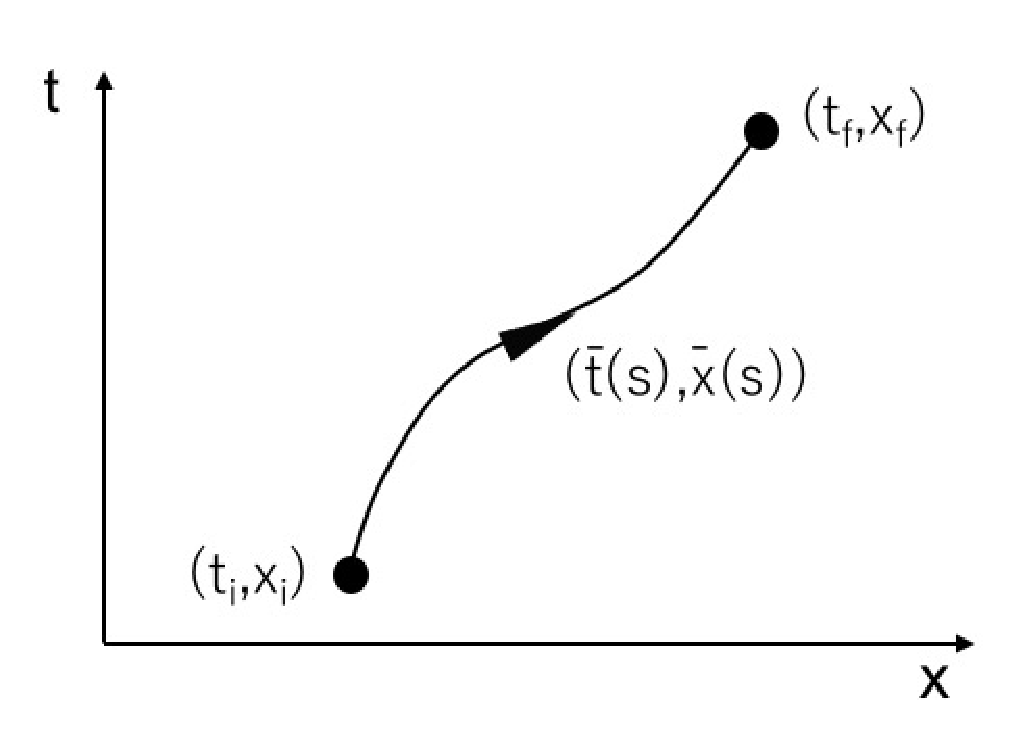
\includegraphics[scale=0.35]{Chapter3-figures/char-c.eps} 
 \end{center}
\caption{Schematic illustration of the characteristic curve.}
\label{fig:char-c}
\end{figure}

The function $f$ can be obtained by integrating the last equation of Eq.(\ref{eq:MCA-4}) 
on the  characteristic curve from the initial point $(t_{\rm i},x_{\rm i})$ to the final point $(t_{\rm f},x_{\rm f})\equiv (t,x)$,
\beq
f(t,x)= f (t_{\rm i}, x_{\rm i}) + h (t, x, t_{\rm i}, x_{\rm i})
\label{eq:MCA-6}
\eeq
where  $h$ stands for an integration of the known function $c(\bar{t},\bar{x})$ on the
characteristic curve.  Eq.(\ref{eq:MCA-6}) implies  that the desired function at $(t,x)$ is obtained 
essential by a "pullback" of the point to $(t_{\rm i},x_{\rm i})$ along the characteristic curve. 
It is a straightforward exercise  to generalize the above derivation to the system with more coordinates,
$(t, \mathbf{x})$.  

%%%%%%%%%%%%%%%%%%%%%%%%%%%%%%%%%%
 \subsubsection*{\center{Leapfrog integrator in molecular dynamics}}
%%%%%%%%%%%%%%%%%%%%%%%%%%%%%%%%%%

Let us start with a Tayler expansion of the field $\phi$:
\beq
\label{eq:LF-phi}
\phi(s+\varepsilon) &=& \phi(s) + \varepsilon \dot{\phi}(s) + \frac{\varepsilon^2}{2} \ddot{\phi}(s) + O(\varepsilon^3), \nonumber \\
&=&  \phi(s) + \varepsilon {\pi}(s) + \frac{\varepsilon^2}{2} \dot{\pi}(s) + O(\varepsilon^3), \nonumber  \\
&=& \phi(s) + \varepsilon {\pi}(s+\varepsilon/2) + O(\varepsilon^3), 
\eeq
where we have used the equation of motion, $\dot{\phi}(s) \equiv d\phi(s)/ds = \pi(s)$.
To evaluate ${\pi}(s+\varepsilon/2)$, we take the midpoint prescription which does not have $O(\varepsilon^2)$ error,
 \beq
 \label{eq:LF-pi}
{\pi}(s+\varepsilon/2)&=&{\pi}(s-\varepsilon/2) + \varepsilon \dot{\pi}(s) + O(\varepsilon^3) \nonumber \\
&=&  {\pi}(s-\varepsilon/2)   - \varepsilon \frac{\delta S(\phi)}{\delta \phi(s)} + O(\varepsilon^3) .
\eeq
Eqs.(\ref{eq:LF-phi}) and (\ref{eq:LF-pi})  give a procedure to move the molecular dynamics one-step forward,
$(\phi(s), \pi(s-\varepsilon/2))  \rightarrow (\phi(s+\varepsilon), \pi(s+\varepsilon/2))$. 
The initial and final steps need to receive special care,
\beq
\pi(\varepsilon/2) = \pi(0) - \frac{1}{2} \varepsilon \frac{\delta S(\phi)}{\delta \phi(s)} + O(\varepsilon^2), \ \ \ 
\pi(s_{\rm f}) =\pi(s_{\rm f}-\varepsilon/2) -  \frac{1}{2} \varepsilon \frac{\delta S(\phi)}{\delta \phi(s_{\rm f})} + 
O(\varepsilon^2),
 \eeq
 which have only $O(\epsilon^2)$ accuracy.  An illustration of this leapfrog integrator is shown in Fig.(\ref{fig:LF}).
 Since the initial and final steps introduce  $O(\varepsilon^2)$ error irrespective of the 
length of the MD trajectory, and  the intermediate steps introduce 
$O(\varepsilon^3) \times \varepsilon^{-1} =O(\varepsilon^2)$ error as a whole,  one finds
 $\Delta H = O(\varepsilon^2)$ after one MD trajectory before the Metropolis test.

The leapfrog integrator satisfies the reversibility and symplectic property, which can be checked explicitly
by using the above definitions (Exercise \ref{prob:13}).
 
 \begin{figure}[t]
\begin{center}
%\framebox[74mm]{\rule[-26mm]{0mm}{52mm}}
%\includegraphics[scale=0.6]{as-scale.eps}
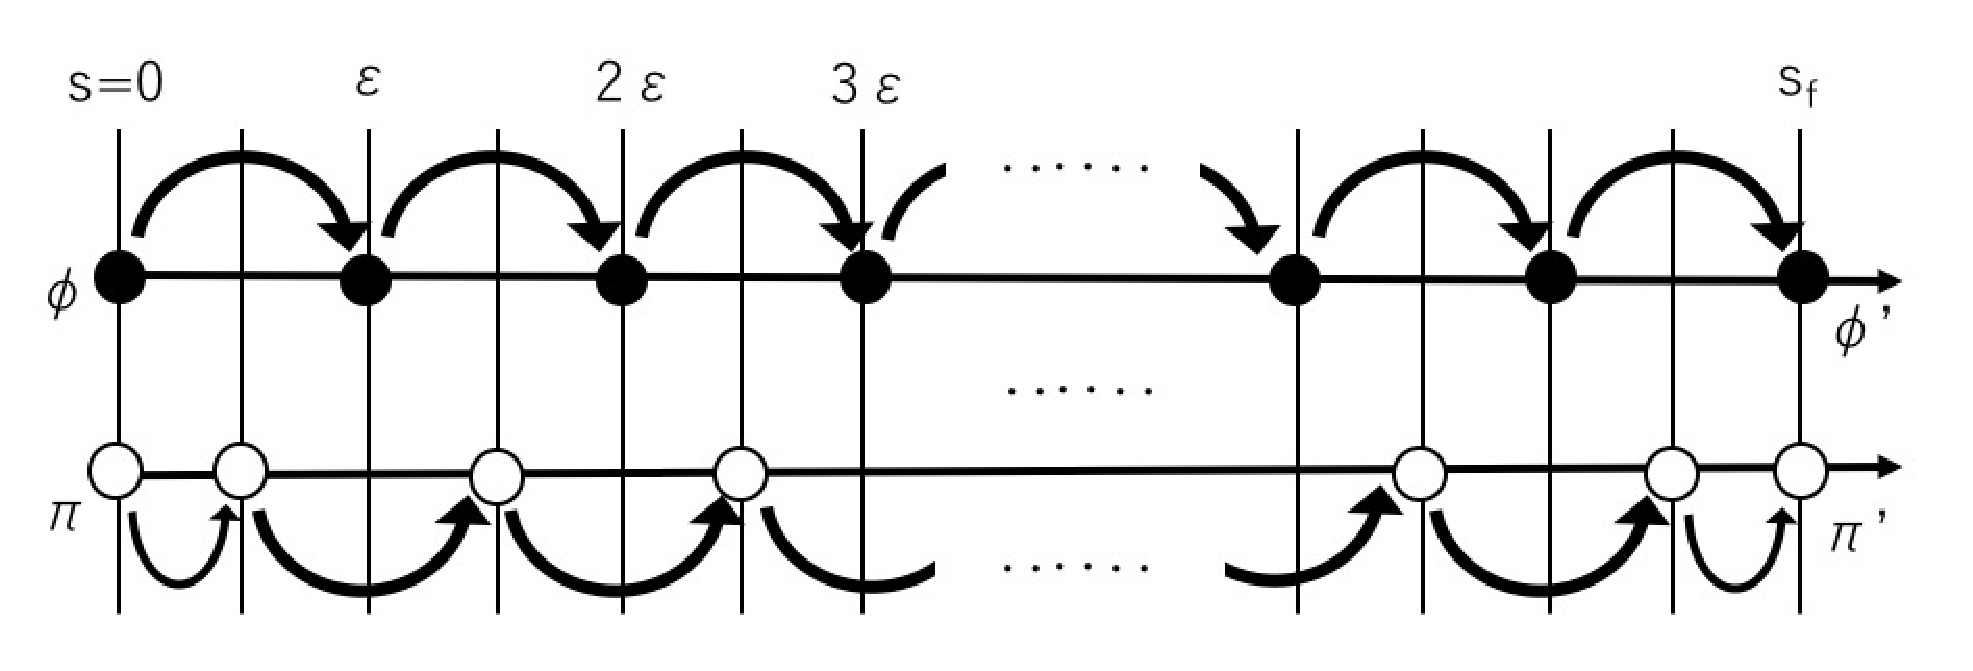
\includegraphics[scale=0.3]{Chapter3-figures/leapfrog.eps} 
 \end{center}
\caption{The leapfrog integrator.}
\label{fig:LF}
\end{figure}


%%%% references %%%%%%%%%
\begin{thebibliography}{99.}%

\bibitem{Wilson:1974sk}
  K.~G.~Wilson, Phys.\ Rev.\ D {\bf 10},  2445  (1974)
  
 \bibitem{Creutz:1980zw}
  M.~Creutz, Phys.\ Rev.\ D {\bf 21},  2308 (1980) 
  
  \bibitem{Brambilla:2014jmp}
  N.~Brambilla {\it et al.}, Eur.\ Phys.\ J.\ C {\bf 74},  2981 (2014)
   
  \bibitem{Wilson:2004de}
  K.~G.~Wilson,  Nucl.\ Phys.\ Proc.\ Suppl.\  {\bf 140},  3 (2005)
  
\bibitem{Creutz:1984mg}
  M.~Creutz, {\em Quarks, gluons and lattices} (Cambridge University Press, 1985)
    
\bibitem{Rothe:1992nt}
  H.~J.~Rothe, World Sci.\ Lect.\ Notes Phys.~{\bf 82}, 1 (2012)

 \bibitem{Hoelbling:2014uea}
  C.~Hoelbling, Acta Phys.\ Polon.\ B {\bf 45},   2143 (2014)


 \bibitem{Ukawa:2015eka}
  A.~Ukawa, J.\ Statist.\ Phys.\  {\bf 160},  1081 (2015)
 
\bibitem{Negele:1988vy}
  J.~W.~Negele and H.~Orland,
 {\em Quantum Many Particle Systems} (Addison-Wesley, 1988)   

\bibitem{Haggstrom:2002}
  O. H\"{a}ggstr\"{o}m,
  {\em Finite Markov Chains and Algorithmic Applications} (Cambridge University Press, 2002)

\bibitem{SuwaTodo:2010}
 H. Suwa and S.Todo,
 Phys.\ Rev.\ Lett.\ {\bf 105},  120603 (2010)

 \bibitem{Duane:1987de}
  S.~Duane, A.~D.~Kennedy, B.~J.~Pendleton and D.~Roweth, Phys.\ Lett.\ B {\bf 195},  216 (1987)

  
\bibitem{Metropolis_1953}
 N. Metropolis, A. W. Rosenbluth, M. N. Rosenbluth, A. H. Teller and E. Teller, J. Chem. Phys. {\bf 21},  1087 (1953)
  
\bibitem{Schaefer:2012tq}
  S.~Schaefer, PoS {\bf LATTICE2012},  001 (2012)
  
 \bibitem{Bali:2000gf}
  G.~S.~Bali, Phys.\ Rept.\  {\bf 343},  1 (2001)

\bibitem{Durr:2008zz}
  S.~Durr {\it et al.}, Science {\bf 322},  1224 (2008)
  
\bibitem{Borsanyi:2014jba}
  S.~Borsanyi {\it et al.}, Science {\bf 347},  1452 (2015)
  
\bibitem{RPP}   
The Review of Particle Physics (2015), \url{http://pdg.lbl.gov/ } 
  
\bibitem{Asakawa:2000tr}
  M.~Asakawa, T.~Hatsuda and Y.~Nakahara,
  Prog.\ Part.\ Nucl.\ Phys.\  {\bf 46} (2001) 459

  
\bibitem{Fodor:2012gf}
  Z.~Fodor and C.~Hoelbling, Rev.\ Mod.\ Phys.\  {\bf 84},  449 (2012)
   
\bibitem{this_book}
Consult other chapters of this volume
 
 \bibitem{Machleidt:2007ms}
  R.~Machleidt, arXiv:0704.0807

\bibitem{Aoki:2013ldr}
  S.~Aoki {\it et al.},
  Eur.\ Phys.\ J.\ C {\bf 74},  2890 (2014)

\bibitem{luescher}
 M.~L\"{u}scher, Nucl. \ Phys.\ B {\bf 354},  531 (1991)

\bibitem{Ishii:2006ec}
N.~Ishii, S.~Aoki and T.~Hatsuda,
Phys.\ Rev.\ Lett.\  {\bf 99},  022001 (2007)

\bibitem{HALQCD:2012aa}
  N.~Ishii {\it et al.} [HAL QCD Collaboration],
 Phys.\ Lett.\ B {\bf 712},  437 (2012)

\bibitem{Iritani:2015dhu}
T.~Iritani [HALQCD Collaboration], arXiv:1511.05246

\bibitem{okubo}
S. Okubo S, R.E. Marshak, Ann. of Phys. {\bf 4},  166 (1958)

\bibitem{Oka-Fujiwara}
M. Oka, K. Shimizu, K. Yazaki, Prog.\ Theor.\ Phys.\ Suppl.\  {\bf 137},   1 (2000)

\bibitem{Inoue:2011ai}
  T.~Inoue {\it et al.} [HAL QCD Collaboration],
  Nucl.\ Phys.\ A {\bf 881},  28 (2012)
  
  \bibitem{Inoue:2013nfe}
  T.~Inoue {\it et al.} [HAL QCD Collaboration],
  Phys.\ Rev.\ Lett.\  {\bf 111},  112503 (2013)
  
 \bibitem{Akmal:1998cf}
  A.~Akmal, V.~R.~Pandharipande and D.~G.~Ravenhall,
  Phys.\ Rev.\ C {\bf 58}, 1804 (1998)
  
  \bibitem{Doi:2015oha}
  T.~Doi {\it et al.} [HAL QCD Collaboration], arXiv:1512.01610
 


  
\end{thebibliography}

\title{Theoretical aspects of few-body systems and effective field theories}
\author{Hans-Werner Hammer}
\institute{Hans-Werner Hammer \at Name of institution and address, \email{name@email.address}}
\maketitle
\abstract{Each chapter should be preceded by an abstract (10--15 lines long) that summarizes the content. The abstract will appear \textit{online} at \url{www.SpringerLink.com} and be available with unrestricted access. This allows unregistered users to read the abstract as a teaser for the complete chapter. As a general rule the abstracts will not appear in the printed version of your book unless it is the style of your particular book or that of the series to which your book belongs.\newline\indent
Please use the 'starred' version of the new Springer \texttt{abstract} command for typesetting the text of the online abstracts (cf. source file of this chapter template \texttt{abstract}) and include them with the source files of your manuscript. Use the plain \texttt{abstract} command if the abstract is also to appear in the printed version of the book.}
%\maketile

\section{General Introduction}
\section{More stuff}


\begin{acknowledgement}
If you want to include acknowledgments of assistance and the like at the end of an individual chapter please use the \verb|acknowledgement| environment -- it will automatically render Springer's preferred layout.
\end{acknowledgement}

\label{chap:chapter5}
\newcommand\mpi {m_{\pi}}
%\newcommand\qslash {\slashed{q}}
%\newcommand{\note}[1]{{\bf \textcolor{red}{\uppercase{#1}}}}
\newcommand\pslash {\slashed{p}}
\newcommand\dslash {\slashed{\partial}}
%\newcommand\Dslash {\slashed{D}}
\newcommand\psidag{\psi^{\dagger}}
\newcommand\tautoinfty{\underset{\tau \to\infty}{\longrightarrow}}
\newcommand\Eq[1]{Eq.~(\ref{eq:#1})}
\newcommand\Eqs[2]{Eqs.~(\ref{eq:#1},\ref{eq:#2})}
%\newcommand\Eqs[2]{Eqs.~(\ref{eq:#1})-(\ref{eq:#2})}
\newcommand\Fig[1]{Fig.~\ref{fig:#1}}
\newcommand\Figtwo[2]{Figs.~\ref{fig:#1} and \ref{fig:#2}}
\newcommand\Figs[2]{Figs.~\ref{fig:#1}-\ref{fig:#2}}
\newcommand\Sec[1]{Sec.~\ref{sec:#1}}
\newcommand\Sect[1]{Section~\ref{sec:#1}}
\newcommand\Tab[1]{Table~\ref{tab:#1}}
%\newcommand{\be}{\begin{equation}}
%\newcommand{\ee}{\end{equation}}
%\newcommand\beq{\begin{eqnarray}}
%\newcommand\eeq{\end{eqnarray}} 
\newcommand\eqn[1]{\label{eq:#1}} 
\newcommand\eq[1]{eq.~(\ref{eq:#1})} 
\newcommand\eqstwo[2]{eqs. (\ref{eq:#1},\ref{eq:#2})} 
\newcommand\eqs[2]{eqs. (\ref{eq:#1}-\ref{eq:#2})} 
\newcommand{\vev}[1]{\langle #1 \rangle}
\newcommand{\lfb}{\bigskip\noindent}
\newcommand{\bfn}{{\mathbf n}}
\newcommand{\bfx}{{\mathbf x}}
\newcommand{\bfr}{{\mathbf r}}
\newcommand{\bfk}{{\mathbf k}}
\newcommand{\bfq}{{\mathbf q}}
\newcommand{\bfp}{{\mathbf p}}
\newcommand{\bfP}{{\mathbf P}}
\newcommand\Ncfg{N_{\mbox{\tiny cfg}}}
\newcommand{\eV}{{\rm ~eV }}
\newcommand{\keV}{{\rm ~keV }}
\newcommand{\GeV}{{\rm ~GeV }}
\newcommand{\TeV}{{\rm ~TeV }}
\newcommand{\MeV}{{\rm ~MeV }}
\newcommand{\calA}{{\mathcal{ A}}}
\newcommand{\calB}{{\mathcal{ B}}}
\newcommand{\calC}{{\mathcal{ C}}}
\newcommand{\calD}{{\mathcal{ D}}}
\newcommand{\calE}{{\mathcal{ E}}}
\newcommand{\calF}{{\mathcal{ F}}}
\newcommand{\calI}{{\mathcal{ I}}}
\newcommand{\calH}{{\mathcal{ H}}}
\newcommand{\calO}{{\mathcal{ O}}}
\newcommand{\calM}{{\mathcal{ M}}}
\newcommand{\calN}{{\mathcal{ N}}}
\newcommand{\calP}{{\mathcal{ P}}}
\newcommand{\calR}{{\mathcal{ R}}}
\newcommand{\calG}{{\mathcal{ G}}}
\newcommand{\calQ}{{\mathcal{ Q}}}
\newcommand{\calS}{{\mathcal{ S}}}
\newcommand{\calT}{{\mathcal{ T}}}
\newcommand{\calU}{{\mathcal{ U}}}
\newcommand{\calV}{{\mathcal{ V}}}
\newcommand{\calW}{{\mathcal{ W}}}
\newcommand{\calZ}{{\mathcal{ Z}}}
\newcommand{\calL}{{\mathcal{ L}}}
\newcommand\rf[1]{{\bf [REF #1]}}
\newcommand{\Tr}{{\rm Tr\,}}
\newcommand\half{{\textstyle{\frac{1}{2}}}} 
\newcommand\fourth{{\textstyle{\frac{1}{4}}}} 
\newcommand\expect[3]{\langle #1|#2|#3\rangle}

%
% Young Tableaux:
%
\newcommand{\mybar}[1]%
        {\kern 0.6pt\overline{\kern -0.6pt#1\kern -0.6pt}\kern 0.6pt}
\newcommand{\drawsquare}[2]{\hbox{%
\rule{#2pt}{#1pt}\hskip-#2pt%  left vertical
\rule{#1pt}{#2pt}\hskip-#1pt%  lower horizontal
\rule[#1pt]{#1pt}{#2pt}}\rule[#1pt]{#2pt}{#2pt}\hskip-#2pt%  upper horizontal
\rule{#2pt}{#1pt}}% right vertical
\newcommand{\Yfund}{\raisebox{-.5pt}{\drawsquare{6.5}{0.4}}}%  fund
\newcommand{\Ybarfund}{\mybar{\raisebox{-.5pt}{\drawsquare{6.5}{0.4}}}}%

%\begin{document}
\title{Lattice methods and effective field theory}
\author{Amy Nicholson}
\institute{Amy Nicholson \at Department of Physics, University of California, Berkeley, Berkeley CA 94720, USA, \email{anicholson@berkeley.edu}}
\maketitle
\abstract{Lattice field theory is a non-perturbative tool for studying properties of strongly interacting field theories, which is particularly amenable to numerical calculations and has quantifiable systematic errors. In these lectures we apply these techniques to nuclear Effective Field Theory (EFT), a non-relativistic theory for nuclei involving the nucleons as the basic degrees of freedom. The lattice formulation of \cite{EKLN1,EKLN4} for so-called pionless EFT is discussed in detail, with portions of code included to aid the reader in code development. Systematic and statistical uncertainties of these methods are discussed at length, and extensions beyond pionless EFT are introduced in the final Section.}
\unitlength = 1mm


\section{\label{sec:intro}Introduction}
Quantitative understanding of nuclear physics at low energies from first principles remains one of the most challenging programs in contemporary theoretical physics research. While physicists have for decades used models combined with powerful numerical techniques to successfully reproduce known nuclear structure data and make new predictions, currently the only tools available for tackling this problem that have direct connections to the underlying theory, Quantum Chromodynamics (QCD), as well as quantifiable systematic errors, are Lattice QCD and Effective Field Theory (EFT). Combined, these techniques may be used to not only quantify any bias introduced when altering QCD in order to make it computationally tractable, but also to better understand the connection between QCD and nuclear physics.

The lattice is a tool for discretizing a field theory in order to reduce the path integral, with an infinite number of degrees of freedom, to a finite-dimensional ordinary integral. By rendering the dimension finite (though extremely large), the integral may then be estimated on a computer using Monte Carlo methods. Errors introduced through discretization and truncation of the region of spacetime sampled are controlled through the spatial and temporal lattice spacings, $b_s,b_{\tau}$, and the spatial and temporal lengths, $L,\beta$. Thus, these errors may be quantified through the lattice spacing dependence of the observables, and often may be removed through extrapolation to the continuum and infinite volume limits.

LQCD is a powerful and advanced tool for directly calculating low-energy properties of QCD. However, severe computational issues exist when calculating properties of systems with nucleons. Unfortunately, these problems grow rapidly with the number of nucleons in the system. 

The first issue is the large number of degrees of freedom involved when using quark fields to create nucleons. In order to calculate a correlation function for a single nucleon in LQCD using quarks (each of which has twelve internal degrees of freedom given by spin and color), one has to perform all possible Wick contractions of the fields in order to build in fermion antisymmetrization. For example, to create a proton using three valence quark operators requires the calculation of two different terms corresponding to interchanging the two up quark sources. The number of contractions involved for a nuclear correlation function grows with atomic number $Z$ and mass number $A$ as $(A+Z)!(2A-Z)!$. For He$_4$ this corresponds to $\sim 5 \times 10^5$ terms\footnote{This is a very na\"ive estimate; far more sophisticated algorithms exist with power-law scaling.}!

The second major problem occurs when performing a stochastic estimate of the path integral. A single quark propagator calculated on a given gauge field configuration may be a part of either a light meson or a heavy nucleon. However, the difference cannot be determined until correlations with the other quark fields present are built in by summing over a sufficiently large number of these field configurations\footnote{This interpretation of the signal-to-noise problem has been provided by David B. Kaplan.}. This leads to large fluctuations from configuration to configuration, and a stochastic signal-to-noise ratio, $\calR$, which degrades exponentially with the number of nucleons in the system,
\beq
\calR \sim e^{-A(M-3/2 m_{\pi})\tau} \ ,
\eeq
where $M$ is the nucleon mass and $m_{\pi}$ is the pion mass \cite{Lepage:1989hd}. This is currently the major limiting factor for the size of nuclear which can be probed using LQCD. The best calculations we have from LQCD using multiple nucleons to date are in the two-nucleon sector \cite{Berkowitz:2015eaa,Kurth:2015cvl,Nicholson:2015pys,Orginos:2015aya,Detmold:2015daa,Chang:2015qxa,Beane:2015yha,Beane:2014sda,Beane:2014ora,Beane:2013br,Beane:2012vq,Beane:2011iw,Beane:2009py,Yamazaki:2015vjn,Yamazaki:2015asa,Yamazaki:2013rna,Yamazaki:2012fn,Yamazaki:2012hi,Doi:2015uvd,Doi:2015oha,Ishii:2006ec,Murano:2013xxa,Aoki:2014mia,Murano:2013gta,HALQCD:2012aa,Inoue:2010hs}, while fewer calculations have been performed for three and four nucleon systems \cite{Beane:2009gs,Beane:2012vq,Beane:2014ora,Beane:2014sda,Chang:2015qxa,Yamazaki:2015vjn,Yamazaki:2015asa,Yamazaki:2013rna,Yamazaki:2012fn,Yamazaki:2012hi,Doi:2011gq}; however, even for two nucleon systems unphysically large pion masses must be used in order to reduce the noise problem. We will discuss signal-to-noise problems in more detail in \Sec{SNR}. 

Starting from an EFT using nucleons as the fundamental degrees of freedom greatly reduces the consequences from both of these issues. EFTs also enjoy the same benefit as the lattice over traditional model techniques of having quantifiable systematic errors, this time controlled by the cutoff of the EFT compared to the energy regime studied. For chiral EFTs this scale is generally $\Lambda_{\chi} \sim m_{\rho} \sim 700$ MeV. Systematic errors can be reduced by going to higher orders in an expansion of $p/\Lambda_{\chi}$, where $p$ is the momentum scale probed, with the remaining error given by the size of the first order which is not included. In a potential model there is no controlled expansion, and it is generally unknown how much the results will be affected by leaving out any given operator. In addition, field theories provide a rigorous mathematical framework for calculating physical processes, and can be directly translated into a lattice scheme.

Our discussion will begin with understanding a very basic nuclear EFT, pionless EFT, at leading order. We will then proceed to discretize this theory and set up a framework for performing Monte Carlo calculations of our lattice theory. We will then discuss how to calculate observables using the lattice theory, and how to understand their associated statistical uncertainties. Next we will discuss quantifying and reducing systematic errors. Then we will begin to add terms to our theory going beyond leading order pionless EFT. Finally, we will discuss remaining issues and highlight some successes of the application of these methods by several different groups.

\section{Basics of Effective Field Theory and Lattice Effective Field Theory}
\subsection{\label{sec:EFT}Pionless Effective Field Theory}
The EFT philosophy that we will follow is to write down all possible operators involving the relevant degrees of freedom within some energy range (determined by the cutoff) that are consistent with the symmetries of the underlying theory. Each operator will be multiplied by an unknown low-energy constant which may be fixed by comparing an observable with experiment or lattice QCD. In order to reduce this generally infinite number of operators to a finite number we must also establish a power-counting rule for neglecting operators that do not contribute within some desired accuracy. This is a notoriously difficult problem for nuclear physics, and is in general observable and renormalization scheme dependent. Here, we will only briefly touch upon two common power-counting schemes, the so-called Weinberg and KSW expansions \cite{Weinberg:1990rz,Weinberg:1991um,Kaplan:1996xu,Kaplan:1998tg,Kaplan:1998we}. For reviews of these and other power-counting schemes, see \cite{Epelbaum:2008ga,Epelbaum:2010nr,Machleidt:2011zz}.

The simplest possible nuclear EFT involves non-relativistic nucleon fields interacting via delta functions. This is known as a pionless EFT, and is only relevant for energy scales up to a cutoff $\Lambda \sim m_{\pi}$. Below this scale, the finite range of pion exchange cannot be resolved, and all interactions appear to be point-like. In this discussion we will closely follow that of Ref.~\cite{Kaplan:2005es}. For the moment, let's just consider a theory of two-component (spin up/down) fermion fields, $\psi$, with the following Lagrangian,
\beq
\label{eq:leff}
\mathcal{L}_{\mbox{\tiny eff}} = \psi^{\dagger}\left( i \partial_{\tau} + \frac{\nabla^2}{2M}\right) \psi + g_0 \left(\psi^{\dagger}\psi\right)^2 + \frac{g_2}{8}\left[ \left(\psi\psi\right)^{\dagger}\left(\psi\overleftrightarrow{\nabla}^2\psi\right)+ \mbox{\tiny h.c.}\right]+\cdots \ ,
\eeq
where
\beq
\overleftrightarrow{\nabla}^2 \equiv \overleftarrow{\nabla}^2-2\overleftarrow{\nabla} \cdot \overrightarrow{\nabla}+\overrightarrow{\nabla}^2 \ ,
\eeq
$M$ represents the nucleon mass, $g_0, g_2, \ldots$ are unknown, low-energy constants (LECs) which may be fixed by comparing to experimental or LQCD results, and all spin indices are suppressed. Because the effective theory involves dynamical degrees of freedom that are only relevant up to a certain scale, we must define a cutoff, $\Lambda$, above which the theory breaks down. In general, the LECs scale as $\Lambda^{-\mbox{\tiny dim}(\mathcal{O})}$, where dim$(\mathcal{O})$ represents the dimension of the operator associated with the LEC. According to na\"ive power counting, the $g_2$ term in \Eq{leff} should be suppressed relative to the $g_0$ term, because adding a derivative to an operator increases its dimension. One should be careful in practice, however, because na\"ive power counting does not always hold, as we will see several times throughout these lectures. 

\subsubsection{\label{sec:scatamp}Two particle scattering amplitude}
In order to set the coefficients $g_0, g_2, \ldots$, we may look to experimental scattering data. In particular, if we wish to set the $g_0$ coefficient we should consider two-particle $s$-wave scattering because the operator associated with $g_0$ contains no derivatives. $g_2$ and other LECs may be set using $p$- and higher-wave scattering data. Recall that the S-matrix for non-relativistic scattering takes the following form:
\beq
S=1+\frac{iMp}{2\pi}A \ ,
\eeq
where $p$ is the scattering momentum and $A$ is the scattering amplitude. For $s$-wave scattering the amplitude may be written as,
\beq
\label{eq:Apcotd}
A=\frac{4\pi}{M} \frac{1}{p\cot\delta - ip} \ ,
\eeq
where $\delta$ is the $s$-wave scattering phase shift. Given a short-range two-body potential, the scattering phase shift has a well-known expansion for low momenta, called the effective range expansion,
\beq
\label{eq:ere}
p\cot\delta = -\frac{1}{a}+\frac{1}{2}r_0p^2+r_1p^4+\cdots \ ,
\eeq
where $a$ is the scattering length, $r_0$ is the effective range, and $r_1$ and higher order terms are referred to as shape parameters. The effective range and shape parameters describe the short-range details of the potential, and are generally of order of the appropriate power of the cutoff in a naturally tuned scenario. 

The scattering length may be used to describe the asymptotic behavior of the radial wavefunction. In particular, consider two-particles interacting via an attractive square-well potential. If the square-well is sufficiently strongly attractive, the wavefunction turns over and goes to zero at some finite characteristic length. This means the system is bound and the size of the bound state is given by the scattering length, $a$. On the other hand, if the wavefunction extends over infinite space, then the system is in a scattering state and the scattering length may be determined as the distance from the origin where the asymptote of the wavefunction intersects the horizontal axis (see \Fig{a0}). This implies that the scattering length in the case of a scattering state is negative. If the potential is tuned to give a system which is arbitrarily close to the crossover point from a bound state to a scattering state, corresponding to infinite scattering length, the state is described as being near unitarity, because the unitarity bound on the scattering cross section is saturated at this point. Note that this implies that the scattering length may be any size and is not necessarily associated with the scale set by the cutoff. However, such a scenario requires fine-tuning of the potential. Such fine-tuning is well-known to occur in nuclear physics, with the deuteron and neutron-neutron $s$-wave scattering being notable examples.

\begin{figure}
\caption{\label{fig:a0}Sketches of two-body radial wavefunctions vs. $r$ corresponding to various scattering lengths. From left to right: $a<0$, $a\to\infty$,$a>0$.}
\includegraphics[width=0.3\linewidth]{Chapter5-figures/al0.png}
\includegraphics[width=0.3\linewidth]{Chapter5-figures/ae0.png}
\includegraphics[width=0.3\linewidth]{Chapter5-figures/ag0.png}
\end{figure}

A many-body system composed of two-component fermions with an attractive interaction is known to undergo pairing between the species (higher $N$-body interactions are prohibited by the Pauli exclusion principle), such as in neutron matter, found in the cores of neutron stars, which is composed of spin up and spin down neutrons. At low temperature, these bosonic pairs condense into a coherent state. If the interaction is only weakly attractive, the system will form a BCS state composed of widely separated Cooper pairs, where the average pair size is much larger than the average interparticle spacing. On the other hand, if the interaction is strongly attractive then the pairs form bosonic bound states which condense into a Bose-Einstein condensate. The crossover between these two states corresponds to the unitary regime, and has been studied extensively in ultracold atom experiments, where the interaction between atoms may be tuned using a Feschbach resonance. In this regime, the average pair size is equal to the interparticle spacing (given by the inverse density), which defines the only scale for the system. Thus, all dimensionful observables one wishes to calculate for this system are determined by the appropriate power of the density times some dimensionless constant. 

\subsubsection{\label{sec:couplings}Two-body LECs}
Returning to our task of setting the couplings using scattering parameters as input, we might consider comparing \Eq{leff} and \Eq{ere}, to determine the LEC $g_0$ using the scattering length, $g_2$ using the effective range, and so forth. To see how this is done in practice we may compute the scattering amplitude $A$ in the effective theory, and match the coefficients to the effective range expansion. Let's begin using only the first interaction term in the effective theory, corresponding to $g_0$. Diagrammatically, the scattering amplitude may be written as the sum of all possible bubble diagrams (see \Fig{bubblesum}). Because the scattering length may take on any value, as mentioned previously, we cannot assume that the coupling $g_0$ is small, so we should sum all diagrams non-perturbatively. The first diagram in the sum is given by the tree level result, $g_0$. If we assume that the system carries energy $E=p^2/M$, then the second diagram may be labeled as in \Fig{loop}, and gives rise to the loop integral,
\beq
\label{eq:loop}
I_0 = i\int \frac{d^4q}{(2\pi)^4}\frac{1}{\left(E/2+q_0-\frac{q^2}{2M}-i\epsilon\right)\left(E/2-q_0-\frac{q^2}{2M}+i\epsilon\right)} \ .
\eeq 
Performing the integral over $q_0$ and the solid angle gives
\beq
\label{eq:loopEFT}
I_0 &=& \frac{1}{2\pi^2}\int^{\pi\Lambda/2} dq\frac{q^2}{\left(E-\frac{q^2}{M}\right)} \\
&=& \frac{M}{2\pi^2}\left[\frac{\pi\Lambda}{2}-\sqrt{ME}\tanh^{-1}\left(\frac{\Lambda}{\sqrt{ME}}\right)\right] \ ,
\eeq
where I have introduced a hard momentum cutoff, $\Lambda$. Removing the cutoff by taking it to infinity results in
\beq
I_0 \underset{\Lambda\to\infty}{\longrightarrow}\frac{M}{4\pi}\left[\Lambda+ip\right] \ .
\eeq
Because the interaction is separable, the $n$th bubble diagram is given by $n$ products of this loop function. Thus, the scattering amplitude is factorizable, and may be written
\beq
\label{eq:Abubble}
A&=&g_0\left[1+\sum_n\left(g_0I_0\right)^n\right] \\
&=& \frac{g_0}{1-g_0I_0} \ .
\eeq
We may now compare \Eqs{Apcotd}{ere} and \Eq{Abubble} to relate the coupling $g_0$ to the scattering phase shift. This is easiest to do by equating the inverse scattering amplitudes,
\beq
\frac{1}{A} &=& \frac{1}{g_0}-\frac{M}{4\pi}\Lambda -\frac{iMp}{4\pi} = -\frac{M}{4\pi a}-\frac{iMp}{4\pi} \ ,
\eeq
where I have used \Eq{ere} cut off at leading order. We now have the relation
\beq
g_0 = \frac{4\pi}{M} \frac{1}{\Lambda-1/a} 
\eeq
between the coupling and the physical scattering length. 

\begin{figure}
\caption{\label{fig:bubblesum}Two-body scattering amplitude represented as a sum of bubble diagrams corresponding to a single contact interaction with coupling $g_0$.}
\includegraphics[width=\linewidth]{Chapter5-figures/simple1}
\end{figure}

\begin{figure}
\caption{\label{fig:loop}Feynman diagram for a single bubble in \Fig{bubblesum}, giving rise to the loop integral \Eq{loop}.}
\includegraphics[width=\linewidth]{Chapter5-figures/loop1}
\end{figure}

Note that the coupling runs with the scale $\Lambda$; the particular dependence is determined by the regularization and renormalization scheme chosen. In order to understand the running of the coupling we may examine the beta function. To do so we first define a dimensionless coupling,
\beq
\hat{g}_0 \equiv -\frac{M\Lambda}{4\pi}g_0 \ ,
\eeq
then calculate
\beq
\label{eq:beta}
\beta\left(\hat{g}_0\right) \equiv \Lambda \frac{\partial \hat{g}_0}{\partial \Lambda} = -\frac{a\Lambda}{\left(a\Lambda-1\right)^2} = -\hat{g}_0\left(\hat{g}_0-1\right) \ .
\eeq
This function is a simple quadratic that is plotted in \Fig{beta}. The beta function has two zeroes, $\hat{g}_0 = 0,1$, corresponding to fixed points of the theory. At a fixed point, the coupling no longer runs with the scale $\Lambda$, and the theory is said to be scale-invariant (or conformal, given some additional conditions). This means that there is no intrinsic scale associated with the theory. The fixed point at $\hat{g}_0=0$ is a trivial fixed point, and corresponds to a non-interacting, free field theory (zero scattering length). The other, non-trivial fixed point at $\hat{g}_0=1$ corresponds to a strongly interacting theory with infinite scattering length; this is the unitary regime mentioned previously. Here, not only does the scattering length go to infinity, as does the size of the radial wavefunction, but the energy of the bound state (as approached from $\hat{g}_0 > 1$) goes to zero and all relevant scales have vanished. Note that this is an unstable fixed point; the potential must be finely tuned to this point or else the theory flows away from unitarity as $\Lambda \to 0$ (IR limit).

\begin{figure}
\caption{\label{fig:beta}Beta function (\Eq{beta}) for the two-body contact interaction. Arrows represent the direction of flow toward the IR.}
\includegraphics[width=0.5\linewidth]{Chapter5-figures/beta.pdf}
\end{figure}

Generally perturbation theory is an expansion around free field theory, corresponding to a weak coupling expansion. This is the approach used as part of the Weinberg power counting scheme for nuclear EFT \cite{Weinberg:1990rz,Weinberg:1991um}. However, in some scattering channels of interest for nuclear theory the scattering length is indeed anomalously large, such as the $^1S_0$ and $^3S_1$ nucleon-nucleon scattering channels, where
\beq
a_{^1S_0} &\sim& -24 \mbox{ fm} \ , \\
a_{^3S_1} &\sim& 5 \mbox{ fm} \ .
\eeq
Such large scattering lengths suggest that an expansion around the strongly coupled fixed-point of unitarity may be a better starting point and lead to better convergence. This approach was taken by Kaplan, Savage, and Wise and led to the KSW power-counting scheme \cite{Kaplan:1998we,Kaplan:1998tg,Kaplan:1996xu}. Unfortunately, nuclear physics consists of many scales of different sizes and a consistent power-counting framework with good convergence for all observables has yet to be developed; in general the convergence of a given scheme depends on the scattering channels involved. 

Because nuclear physics is not weakly coupled in all channels, non-perturbative methods, such as lattice formulations, will be favorable for studying few- and many-body systems, where two-body pairs may interact through any combination of channels simultaneously. Due to the scale-invariant nature of the unitary regime, it provides a far simpler testbed for numerical calculations of strongly-interacting theories, so we will often use it as our starting point for understanding lattice EFT methods. 

\subsection{\label{sec:LEFT}Lattice Effective Field Theory}

Our starting point for building a lattice EFT will be the path integral formulation of quantum field theory in Euclidean spacetime. The use of Euclidean time allows the exponent of the path integral to be real (in certain cases), a property which will be essential to our later use of stochastic methods for its evaluation. Given a general theory for particles $\psi,\psi^{\dagger}$ obeying a Lagrangian density \beq 
\mathcal{L}(\psi^{\dagger},\psi) = \psi^{\dagger}\left( \partial_{\tau}-\mu \right)\psi+ \mathcal{H}\left[\psi^{\dagger}, \psi\right] \ ,
\eeq
where $\tau$ is the Euclidean time, $\mu$ the chemical potential, and $\mathcal{H}$ is the Hamiltonian density, the Euclidean path integral is given by
\beq
Z=\int \mathcal{D} \psi^{\dagger}\mathcal{D} \psi e^{-\int d\tau d^3x\left[\mathcal{L}(\psi^{\dagger},\psi)\right]} \ .
\eeq
If the integral over Euclidean time is compact, then the finite time extent $\beta$ acts as an inverse temperature, and we may draw an analogy with the partition function in statistical mechanics, $Z = tr\left[e^{-H\beta}\right]$. This analogy is often useful when discussing lattice formulations of the path integral. In this work we will generally consider $\mu=0$ and create non-zero particle density by introducing sources and sinks for particles and calculating correlation functions. 

We discretize this theory on a square lattice consisting of $L^3 \times N_{\tau}$ points, where $L$ is the number of points in all spatial directions, and $N_{\tau}$ is the number of temporal points. We will focus on zero temperature physics, corresponding to large $N_{\tau}$\footnote{The explicit condition on $N_{\tau}$ required for extracting zero temperature observables will be discussed in \Sec{observables}}. We must also define the physical distance between points, the lattice spacings $b_s, b_{\tau}$, where $b_{\tau} = b_s^2/M$ by dimensional analysis for non-relativistic theories. The fields are now labeled by discrete points, $\psi(\vec{x},\tau) \to \psi_{\vec{n},\tau}$, and continuous integrals are replaced by discrete sums, $\int d^3x \to \sum_{\vec{n},\tau}^{L,N_{\tau}}$.

\subsubsection{Free field theory}
To discretize a free field theory, we must discuss discretization of derivatives. The simplest operator which behaves as a single derivative in the continuum limit is a finite difference operator,
\beq
\partial_{\hat{k}}^{(L)} f_j = \frac{1}{b_s}\left[f_{j+\hat{k}}-f_j\right] \ ,
\eeq
where $\hat{k}$ is a unit vector in the $k$-direction. The discretized second derivative operator must involve two hops, and should be a symmetric operator to behave like the Laplacian. A simple possibility is
\beq
\nabla_L^2 f_j = \sum_{k} \frac{1}{b_s^2}\left[ f_{j+\hat{k}}+f_{j-\hat{k}}-2 f_j \right] \ .
\eeq
We can check the continuum limit by inspecting the corresponding kinetic term in the action,
\beq
S_{\mbox{\tiny KE}} \propto \sum_j \psi_j^{\dagger} \nabla_L^2 \psi_j \ .
\eeq
The fields may be expanded in a plane wave basis,
\beq
\psi_j = \sum_{k=-L/2}^{L/2} \psi_k e^{-\frac{2\pi i}{L} j \dot k} \ ,
\eeq
for spatial indices, $j$, leading to
\beq
\sum_j \psi_j^{\dagger} \nabla_L^2 \psi_j = \frac{1}{b_s^2}\sum_j \sum_{k'}\sum_k \psi_{k'}^{\dagger} \psi_k \left[ e^{\frac{2\pi i}{L}j \dot k'} e^{\frac{-2\pi i}{L} j\dot k} \right] \left[e^{\frac{-2\pi i}{L}k}+e^{\frac{2\pi i}{L} k}-2\right] \ .
\eeq
After performing the sum over $j$ the first piece in brackets gives $\delta_{kk'}$, while the second is proportional to $\sin^2(k\pi/L)$, resulting in,
\beq
\sum_j \psi_j^{\dagger} \nabla_L^2 \psi_j = -\frac{4}{b_s^2}\sum_k \psi_k^{\dagger}\psi_k \sin^2\left(\frac{k\pi}{L}\right) \ .
\eeq 
Finally, expanding the sine function for small $k/L$ gives,
\beq
\label{eq:kinetic}
\sum_j \psi_j^{\dagger} \nabla_L^2 \psi_j = \sum_k \psi_k^{\dagger}\psi_k &&\left[\underbrace{-\left(\frac{2\pi k}{b_s L}\right)^2+\frac{b_s^2}{12}\left(\frac{2\pi k}{b_s L}\right)^4+ \cdots }\right] \ ,\cr
&& \hspace{6mm} -p^2 + \frac{b_s^2}{12} p^4 + \cdots \underset{b_s\to 0}{\longrightarrow} -p^2 
\eeq
where I've used the finite volume momentum $p = \frac{2\pi k}{b_s L}$ to rewrite the expression in square brackets. Thus, we have the correct continuum limit for the kinetic operator. Note that for larger momenta, approaching the continuum limit requires smaller $b_s$. However, this is only one possibility for a kinetic term. We can always add higher dimension operators (terms with powers of $b_s$ in front of them), in order to cancel leading order terms in the expansion \Eq{kinetic}. This is a form of what's called improvement of the action, and will be discussed in more detail in \Sec{systematic}.

Adding a temporal derivative term, 
\beq
\partial_{\tau}^{(L)} \psi_{\vec{x},\tau} = \frac{1}{b_{\tau}}\left[\psi_{\vec{n},\tau}- \psi_{\vec{n},\tau-1}\right] \ ,
\eeq
we can now write down a simple action for a non-relativistic free-field theory,
\beq
S_{\mbox{\tiny free}} = \sum_{\tau,\tau'} \frac{1}{b_{\tau}}\psi_{\tau'}^{\dagger}\left[K_0\right]_{\tau,\tau'}\psi_{\tau} \ ,
\eeq
where I've defined a matrix $K_0$ whose entries are $L^3 \times L^3$ blocks,
\beq
K_0 \equiv \left(\begin{array}{ccccccc}
D & -1 & 0 & 0 & . & . & . \\
0 & D & -1 & 0 & . & . &.  \\
0 & 0 & D & -1 &  .&.  & . \\
. & .&. &. & . & & \\ 
. & .& .& .& & . & \\ 
1 & .&. & .& & & . \\ 
\end{array} \right)
\eeq
where $D \equiv 1-\frac{b_s^2 \nabla_L^2}{2}$ contains the spatial Laplacian, and therefore connects fields on the same time slice (corresponding to diagonal entries of the matrix $K_0$), while the temporal derivative contributes the off-diagonal pieces. Note that the choice of ``1" in the lower left corner corresponds to anti-periodic boundary conditions, appropriate for fermionic fields. For zero temperature calculations the temporal boundary conditions are irrelevant, and it will often be useful to choose different temporal boundary conditions for computational or theoretical ease. 

\subsubsection{Interactions}
Now let's discuss adding interactions to the theory. We'll focus on the first term in a nuclear EFT expansion, the four-fermion interaction:
\beq
\mathcal{L}_{\mbox{\tiny int}} = g_0 \psi_{n,\uparrow} \psi_{n,\uparrow} \psi_{n,\downarrow} \psi_{n,\downarrow} \ ,
\eeq
where $(\uparrow,\downarrow)$ now explicitly label the particles' spins (or alternatively, flavors). Because anti-commuting fields cannot easily be accommodated on a computer, they must be integrated out analytically. The only Grassmann integral we know how to perform analytically is a Gaussian, so the action must be bilinear in the fields. One trick for doing this is called a Hubbard-Stratonovich (HS) transformation, in which auxiliary fields are introduced to mediate the interaction. The key is to use the identity,
\beq
e^{b_{\tau}g_0\psi_{\uparrow}^{\dagger}\psi_{\uparrow}\psi_{\downarrow}^{\dagger}\psi_{\downarrow}} = \frac{1}{\sqrt{2\pi}}\int_{-\infty}^{\infty}d\phi^{-\phi^2/2-\phi\sqrt{b_{\tau}g_0}\left(\psi_{\uparrow}^{\dagger}\psi_{\uparrow}+\psi_{\downarrow}^{\dagger}\psi_{\downarrow}\right)} \ ,
\eeq
where I have dropped the spacetime indices for brevity. This identity may be verified by completing the square in the exponent on the right hand side and performing the Gaussian integral over the auxiliary field $\phi$. This form of HS transformation has the auxiliary field acting in what is called the density channel $\left(\psi_{\uparrow}^{\dagger}\psi_{\uparrow}+\psi_{\downarrow}^{\dagger}\psi_{\downarrow}\right)$. It is also possible to choose the so-called BCS channel, $\left(\psi_{\uparrow}^{\dagger}\psi_{\downarrow}^{\dagger}+\psi_{\uparrow}\psi_{\downarrow}\right)$, the usual formulation used in BCS models, however this causes a so-called sign problem when performing Monte Carlo sampling, as will be discussed in detail in \Sec{sign}. Transformations involving non-Gaussian auxiliary fields may also be used, such as
\beq
Z_2 \mbox{ field: } &&\frac{1}{2} \sum_{\phi=\pm 1}e^{-\phi\sqrt{b_{\tau}g_0}\left(\psi_{\uparrow}^{\dagger}\psi_{\uparrow}+\psi_{\downarrow}^{\dagger}\psi_{\downarrow}\right)} \cr
\mbox{compact continuous: } && \frac{1}{2\pi} \int_{-\pi}^{\pi}e^{-\sin \phi\sqrt{b_{\tau}g_0}\left(\psi_{\uparrow}^{\dagger}\psi_{\uparrow}+\psi_{\downarrow}^{\dagger}\psi_{\downarrow} \right)}  \ .
\eeq
These formulations may have different pros and cons in terms of computational and theoretical ease for a given problem, and should be chosen accordingly. For example, the $Z_2$ interaction is conceptually and computationally the simplest interaction, however, it also induces explicit $4-$ and higher-body interactions in systems involving more than two-components which may not be desired. 

\subsubsection{Importance sampling}
The action may now be written with both kinetic and interaction terms,
\beq
\label{eq:actiongen}
S=\frac{1}{b_{\tau}}\sum_{\tau,\tau'}\psi_{\tau'}^{\dagger}\left[K(\phi)\right]_{\tau'\tau}\psi_{\tau} \ ,
\eeq
where the matrix $K$ includes blocks which depend on the auxiliary field $\phi$, and also contains non-trivial spin structure that has been suppressed. The partition function can be written
\beq
Z = \int \mathcal{D}\phi \mathcal{D}\psi^{\dagger}\mathcal{D}\psi \rho[\phi]e^{-S[\phi,\psi^{\dagger}\psi]} \ ,
\eeq
where the integration measure for the $\phi$ field, $\rho[\phi]$, depends on the formulation chosen,
\beq
\rho[\phi] = \left\{ \begin{array}{cc}
\prod_n e^{-\phi_n^2/2} & \mbox{Gaussian}\\
\prod_n \frac{1}{2}\left(\delta_{\phi_{n,1}}+\delta_{\phi_{n,-1}}\right) & Z_2 \\
\prod_n \left(\theta(-\pi+\phi_n)\theta(\pi-\phi_n)\right) & \mbox{compact continuous} 
\end{array}\right. \ .
\eeq

With the action in the bilinear form of \Eq{actiongen}, the $\psi$ fields can be integrated out analytically, resulting in
\beq
\label{eq:prob}
Z_{\phi}=\int \calD \phi P[\phi] \qquad P[\phi] \equiv \rho[\phi]\det K[\phi] \ .
\eeq
Observables take the form
\beq
\langle \calO \rangle = \frac{1}{Z} \int \calD \phi P[\phi]\calO[\phi] \ .
\eeq

Through the use of discretization and a finite volume, the path integral has been converted into a standard integral with finite dimension. However, the dimension is still much too large to imagine calculating it on any conceivable computer, so we must resort to Monte Carlo methods for approximation. The basic idea is to generate a finite set of $\phi$ field configurations of size $\Ncfg$ according to the probability measure $P[\phi]$, calculate the observable on each of these configurations, then take the mean as an approximation of the full integral,
\beq
\langle \calO \rangle \approx \frac{1}{\Ncfg}\sum_n^{\Ncfg}\calO(\phi_n) \ .
\eeq
Assuming the central limit theorem holds, for $\Ncfg$ large enough (a non-trivial condition, as will be discussed in \Sec{overlap}), the distribution of the mean approaches a Gaussian, and the error on the mean falls off with the square root of the sample size. 

There are several algorithms on the market for generating field configurations according to a given probability distribution, and I will only briefly mention a few. Lattice calculations are particularly tricky due to the presence of the determinant in \Eq{prob}, which is a highly non-local object and is very costly to compute. One possible algorithm to deal with this is called determinantal Monte  Carlo, which implements local changes in $\phi$, followed by a simple Metropolis accept/reject step. This process can be rather inefficient due to the local updates. An alternative possibility is Hybrid Monte Carlo, commonly used for lattice QCD calculations, in which global updates of the field are produced using molecular dynamics as a guiding principle. Note that the field $\phi$ must be continuous in order to use this algorithm due to the use of classical differential equations when generating changes in the field. Also common in lattice QCD calculations is the use of pseudofermion fields as a means for estimating the fermion determinant. Here the determinant is rewritten in terms of a Gaussian integral over bosonic fields, $\chi$,
\beq
\det K[\phi] \propto \int \calD \chi^{\dagger}\calD \chi e^{-\chi^{\dagger}K^{-1}[\phi]\chi} \ .
\eeq
This integral is then evaluated stochastically. These are just a sample of the available algorithms. For more details on these and others in the context of non-relativistic lattice field theory, see \cite{Drut:2012md}.

\subsubsection{Example formulation}
Now that we have developed a general framework for lattice EFT, let's be explicit and make a few choices in order to further our understanding and make calculations simpler. The first choice I'm going to make is to use a $Z_2$ $\phi$ field, so that $\rho[\phi]$ is trivial. The next simplification I'm going to make is to allow the $\phi$ fields to live only on temporal links,
\beq
\label{eq:pointint}
\calL_{\mbox{\tiny int}} = \sqrt{b_{\tau}g_0}\phi_{x,\tau}\psidag_{x,\tau}\psi_{x,\tau-1} \ .
\eeq
Note that we are free to make this choice, so long as the proper four-fermion interaction is regained in the continuum limit. This choice renders the interaction separable, as it was in our continuum effective theory. This means we may analytically sum two-body bubble chain diagrams as we did previously in order to set the coupling $g_0$ using some physical observable (see \Fig{dimer}). 

With this choice we can now write the $K$-matrix explicitly as
\beq
K[\phi,N_{\tau}] \equiv \left(\begin{array}{ccccccc}
D & -X(\phi_{N_{\tau}-1}) & 0 & 0 & . & . & . \\
0 & D & -X(\phi_{N_{\tau}-2}) & 0 & . & . & . \\
. & .& .& .&  & & \\ 
. & .&. & &. &  & \\ 
. &. & .& & & D & X(\phi_0)\\ 
X(\phi_{N_{\tau}}) & .&. & & &0 & D \\ 
\end{array} \right) \ ,
\eeq
where $X(\phi_\tau) \equiv 1-\sqrt{g_0}\phi_\tau$. Now the $\phi$-dependence exists only on the upper diagonal, as well as the lower left due to the boundary condition. This block will be eliminated through our final choice: open boundary conditions in time for the $\psi$ fields, $X(\phi_{N_{\tau}})=0$. As mentioned previously, we are free to choose the temporal boundary conditions as we please, so long as we only consider zero temperature (and zero chemical potential) observables. 

\begin{figure}
\caption{\label{fig:dimer}Two-body scattering amplitude of \Fig{bubblesum}, where the contact interaction has been replaced in the second line by exchange of a dimer auxiliary field via a Hubbard-Stratonovich transformation.}
\includegraphics[width=\linewidth]{Chapter5-figures/dimer}
\end{figure}

With this set of choices the matrix $K$ consists purely of diagonal elements, $D$, and upper diagonal elements, $X(\phi_\tau)$. One property of such a matrix is that the determinant, which is part of the probability distribution, is simply the product of diagonal elements, $\det K = \prod_{\tau} D$. Note that $D$ is completely independent of the field $\phi$. This means that the determinant in this formulation has no impact on the probability distribution $P[\phi]$, and therefore never needs to be explicitly computed, greatly reducing the computational burden. Thus in all of our calculations, performing the path integral over $\phi$ simply amounts to summing over $\phi = \pm 1$ at each lattice site. 

Finally, this form of $K$ also makes the calculation of propagators very simple. The propagator from time 0 to $\tau$ may be written,
\beq
K^{-1}(\tau,0) &=& D^{-1} X(\phi_{\tau-1})D^{-1}X(\phi_{\tau-2})D^{-1} \cdots X(\phi_0)D^{-1} \cr
&=& D^{-1}X(\phi_{\tau-1})K^{-1}(\tau-1,0) \ ,
\eeq
where $K^{-1}(0,0) = D^{-1}$, and all entries are $V\times V \ , (V=L^3)$ matrices which may be projected onto the desired state. This form suggests a simple iterative approach to calculating propagators: start with a source (a spatial vector projecting onto some desired quantum numbers and interpolating wavefunction), hit it with the kinetic energy operator corresponding to free propagation on the time slice, then hit it with the $\phi$ field operator on the next time link, then another free kinetic energy operator, and so on, finally projecting onto a chosen sink vector. 

As will be discussed further in Sec{systematic}, it is often preferable to calculate the kinetic energy operator in momentum space, while the auxiliary field in $X(\phi)$ must be generated in position space. Thus, Fast Fourier Transforms (FFTs) may be used between each operation to quickly translate between the bases. Example code for generating source vectors, kinetic operators, and interaction operators will be provided in later Sections.

A cartoon of this process on the lattice is shown in \Fig{lat}. The choice of $Z_2$ auxiliary fields also simplifies the understanding of how four-fermion interactions are generated. On every time link, imagine performing the sum over $\phi = \pm 1$. Clearly, if there is only a single fermion propagator on a given link this gives zero contribution because the term is proportional to $\sum_{\phi=\pm 1} \sqrt{g_0} \phi = 0$. However, on time slices where two propagators overlap, we have instead $\sum_{\phi = \pm 1} g_0 \phi^2 = 2 g_0$. In sum, anywhere two fermions exist at the same spacetime point of a factor of $g_0$ contributes, corresponding to an interaction.

\begin{figure}
\caption{\label{fig:lat}Schematic of a lattice calculation for a two-particle correlation function. The two particles (red and blue lines) propagate through the lattice between source $\psi(0)$ and sink $\psi(\tau)$, seeing particular values of the auxiliary field, $\phi$, on each time link. If two particles occupy the same temporal link, then upon summation over all possible values of $\phi$ at each link, a non-zero contribution is generated by the interaction term because $\langle \phi^2 \rangle \neq 0$.}
\includegraphics[width=0.3\linewidth]{Chapter5-figures/lattice.png}
\end{figure}

\subsubsection{\label{sec:tuning}Tuning the two-body interaction}

There are several ways to set the two-body coupling. Here we will explore two methods, using different two-body observables. The first involves calculating the two-particle scattering amplitude, and tuning the coupling to reproduce known scattering parameters, to make a connection with our previous calculation for the effective theory. The second method uses instead the energy spectrum of a two-particle system in a box. This powerful method will be useful later when we begin to improve the theory in order to reduce systematic errors.

We have calculated the scattering amplitude previously for our effective theory using a momentum cutoff. For the first method for tuning the coupling, we will calculate it again using our lattice theory with the lattice cutoff as a regulator. First we need the single particle free propagator:
\beq
\label{eq:oneprop}
G_0(\tau,\vec{p}) &=& \langle \vec{p},\tau | \left(D^{-1}\right)^{\tau+1}|\vec{p},0\rangle = \left(1+\frac{\Delta(p)}{M}\right)^{-(\tau+1)} \ , \cr
\Delta(p) &\equiv& -\frac{1}{2}\langle \vec{p}|\nabla_L^2 | \vec{p}\rangle \cr
&=& \sum_i \sin^2 \frac{p_i}{2} \ ,
\eeq
where I've set $b_s=1$ (we will use this convention from now on until we begin to discuss systematic errors), and have used the previously defined discretized Laplacian operator. I've written the propagator in a mixed $\vec{p},\tau$ representation, as this is often useful in lattice calculations for calculating correlation functions in time when the kinetic operator, $D$, is diagonal in momentum space. 

The diagrammatic two-particle scattering amplitude is shown on the bottom line in \Fig{dimer}. Because we have chosen the interaction to be separable, the amplitude can be factorized:
\beq
\label{eq:aint}
A=g_0\left[1+\sum_n(g_0\hat{L})^n\right] = \frac{g_0}{1-g_0\hat{L}} \ ,
\eeq
where the one loop integral, $\hat{L}$, will be defined below. As before, in order to set a single coupling we need one observable, so we use the effective range expansion for the scattering phase shift to leading order,
\beq
\label{eq:aERE}
A = \frac{4\pi}{M} \frac{1}{p\cot\delta-i p} \approx -\frac{4\pi a}{M} \ .
\eeq
Relating \Eqs{aint}{aERE}, we find
\beq
\label{eq:eigeqscat}
\frac{1}{g_0} = -\frac{M}{4\pi a} + \hat{L} \ .
\eeq

We will now evaluate the loop integral using the free single particle propagators, \Eq{oneprop},
\beq
\hat{L} &=& \frac{1}{V} \sum_{\vec{p}}\sum_{\tau=0}^{\infty} \left[G_0(\tau,\vec{p})\right]^2 \cr
&=& \frac{1}{V} \sum_{\vec{p}}\sum_{\tau=0}^{\infty} \frac{1}{\left(1+\frac{\Delta(p)}{M}\right)^{2\tau+2}} \cr
&=& \frac{1}{V} \sum_{\vec{p}} \frac{1}{\left(1+\frac{\Delta(p)}{M}\right)^2}\left[1+\sum_{\tau=0}^{\infty}\frac{1}{\left[\left(1+\frac{\Delta(p)}{M}\right)^2\right]^\tau}\right] \cr
&=&\frac{1}{V} \sum_{\vec{p}}\frac{M}{2}\frac{1}{\Delta(p)\left(1+\frac{\Delta(p)}{2M}\right)} \ .
\eeq
This final sum may be calculated numerically for a given $M$ and $L$ (governing the values of momenta included in the sum), as well as for different possible definitions of the derivative operators contained in $\Delta$, giving the desired coupling, $g_0$, via \Eq{eigeqscat}.

The second method for setting the coupling utilizes the calculation of the ground state energy of two particles. We start with the two-particle correlation function,
\beq
C_2(\tau) = \frac{1}{Z}\int \calD \phi \calD \psidag \calD \psi e^{-S[\psidag, \psi, \phi]} \Psi^{\dagger}_{\mbox{\tiny src,2}} \Psi_{\mbox{\tiny snk,2}} \ ,
\eeq
where $\Psi_{\mbox{\tiny src,2(snk,2)}}$ is a source (sink) wavefunction involving one spin up and one spin down particle. Integrating out the fermion fields gives,
\beq
C_2(\tau) &=& \frac{1}{Z_{\phi}}\int \calD \phi P[\phi] \langle \Psi_{\mbox{\tiny snk,2}}|K^{-1}(\tau,0) \otimes K^{-1}(\tau,0) | \Psi_{\mbox{\tiny src,2}}\rangle \cr
&=& \frac{1}{4\tau}\sum_{\phi=\pm 1}\langle \Psi_{\mbox{\tiny snk,2}} | D^{-1} \otimes D^{-1} X(\phi_\tau)\otimes X(\phi_{\tau})D^{-1}\otimes D^{-1} X(\phi_{\tau-1})\otimes X(\phi_{\tau-1}) \cdots |\Psi_{\mbox{\tiny src,2}} \rangle \ . \cr
\eeq
I will now write out the components of the matrices explicitly:
\beq
\label{eq:c2xspace}
C_2(\tau) &=& \frac{1}{4\tau}\sum_{x_1 x_2 x_1' x_2' \cdots y_1y_2}\sum_{\phi_{x_1} \phi_{x_1'}\cdots = \pm 1} \langle \Psi_{\mbox{\tiny snk,2}}|x_1 x_2\rangle D^{-1}_{x_1 x_1'}D^{-1}_{x_2 x_2'}(\delta_{x_1 x_1'} + \sqrt{g_0}\phi_{x_1}\delta_{x_1 x_1'})(\delta_{x_2 x_2'} + \sqrt{g_0}\phi_{x_2}\delta_{x_2 x_2'}) \cr
&& \times D^{-1}_{x_1' x_1''}D^{-1}_{x_2 x_2''} \cdots \langle y_1 y_2|\Psi_{\mbox{\tiny src,2}}\rangle  \ .
\eeq
The first (last) piece in angle brackets represents the position space wavefunction created by the sink (source). All $\phi$ fields in \Eq{c2xspace} are uncorrelated, so we can perform the sum for each time slice independently. One such sum is given by,
\beq
&&\frac{1}{4}\sum_{x_1x_1'x_2x_2'}\sum_{\phi_{x_1}\phi_{x_2}} \delta_{x_1x_1'}\delta_{x_2x_2'}(`1+\sqrt{g_0}\phi_{x_1}+\sqrt{g_0}\phi_{x_2}+g_0 \phi_{x_1}\phi_{x_2}) \cr
&=&\sum_{x_1x_2}(1+g_0\delta_{x_1x_2}) \ ,
\eeq
where the cross terms vanish upon performing the sum. If we make the following definitions,
\beq
\langle x_1 x_1' | \calD ^{-1} | x_2 x_2' \rangle \equiv D^{-1}_{x_1 x_1'} D^{-1}_{x_2 x_2'} \ ,  \qquad \langle x_1 x_2 | \calV | x_1' x_2' \rangle \equiv g_0 \delta_{x_1x_1'}\delta_{x_2x_2'}\delta_{x_1x_2}  \ ,
\eeq
then we can write the two-particle correlation function as,
\beq
C_2(\tau) &=& \langle \Psi_{\mbox{\tiny snk,2}}| \calD^{-1}(1+\calV)\calD^{-1}(1+\calV) \cdots \calD^{-1}(1+\calV)\calD^{-1} | \Psi_{\mbox{\tiny src}} \rangle \cr
&=& \langle \Psi_{\mbox{\tiny snk}} | \calD^{-1/2} \calT \calD^{-1/2} | \Psi_{\mbox{\tiny src,2}} \rangle \ ,
\eeq
where I have made the definition
\beq
\label{eq:transmat}
\calT \equiv \calD^{-1/2}(1+\calV) \calD^{-1/2} \ .
\eeq
Recall from statistical mechanics that correlation functions may be written as $\tau$ insertions of the transfer matrix, $e^{-H}$, acting between two states,
\beq
C(\tau) &=& \langle \Psi_{\mbox{\tiny snk,2}} | e^{-H\tau} | \Psi_{\mbox{\tiny src,2}} \rangle \cr 
&=& \langle \Psi_{\mbox{\tiny snk,2}} | \left[e^{-H}\right]^{\tau} | \Psi_{\mbox{\tiny src,2}} \rangle \ .
\eeq 
Then we may identify $\calT$ in \Eq{transmat} as the transfer matrix of the theory, $\calT = e^{-H}$. This in turn implies that the logarithm of the eigenvalues of $\calT$ give the energies of the two-particle system.

We will now evaluate the transfer matrix in momentum space:
\beq
\label{eq:transexplicit}
\langle p q| \calT | p'q'\rangle &=& \sum_{kk'll'}\langle pq|\calD^{-1/2}|kl\rangle \langle kl | 1+\calV | k'l' \rangle \langle k'l' |\calD^{-1/2}|p'q'\rangle \cr
&=& \sum_{kk'll'} \delta_{k'p'}\delta_{l'q'}\delta_{pk}\delta_{ql} \left(\delta_{kk'}\delta_{ll'}+\delta_{k+l,k'+l'} \frac{g_0}{V}\right) \cr
&\times& \left[\frac{1}{\left(1+\frac{\Delta(p)}{M}\right)\left(1+\frac{\Delta(q)}{M}\right)\left(1+\frac{\Delta(p')}{M}\right)\left(1+\frac{\Delta(q')}{M}\right)}\right]^{1/2} \cr
&=&\frac{\delta_{pp'}\delta_{qq'}+\frac{g_0}{V}\delta_{p+q,p'+q'}}{\sqrt{\xi(p)\xi(q)\xi(q')\xi(p')}} \ ,
\eeq
where I have made the definition,
\beq
\xi(p) \equiv 1+\frac{\Delta(q)}{M} \ .
\eeq
The eigenvalues of the matrix $\calT$ may be evaluated numerically to reproduce the entire two-particle spectrum. However, for the moment we only need to set a single coupling, $g_0$, so one eigenvalue will be sufficient. The largest eigenvalue of the transfer matrix, corresponding to the ground state, may be found using a simple variational analysis\footnote{Many thanks to Michael Endres for the following variational argument.}. Choosing a simple trial state wavefunction,
\beq
\langle pq| \Psi \rangle = \frac{\psi(p)}{\sqrt{V}}\delta_{p,-q} \ ,
\eeq
subject to the normalization constraint,
\beq
\frac{1}{V}\sum_p |\psi(p)|^2 = 1 \ ,
\eeq
we now need to maximize the following functional:
\beq
\langle \Psi |\calT | \Psi \rangle = \left[\frac{1}{V} \sum_p \frac{|\psi(p)|^2}{\xi^2(p)} + \frac{g_0}{V^2}\left| \sum_p \frac{\psi(p)}{\xi(p)} \right|^2 + \lambda \left(1-\frac{1}{V}\sum_p |\psi(p)|^2\right)\right] \ ,
\eeq
where $\lambda$ is a Lagrange multiplier enforcing the normalization constraint, and I have used the fact that $\xi(p)$ is symmetric in $p$ to simplify the expression. Taking a functional derivative with respect to $\psidag(q)$ on both sides gives
\beq
-\lambda \psi(q) + \frac{\psi(q)}{\xi^2(q)} + \frac{g_0}{V}\sum_p \frac{\psi(p)}{\xi(p)\xi(q)} = 0 \ ,
\eeq
where I have set the expression equal to zero in order to locate the extrema. Rearranging this equation, then taking a sum over $q$ on both sides gives
\beq
\sum_q\frac{\psi(q)}{\xi(q)} &=& \sum_q \frac{g_0}{V} \frac{1}{\lambda \xi^2(q)-1} \sum_p \frac{\psi(p)}{\xi(p)} \ ,
\eeq
finally resulting in
\beq
\label{eq:eigeqlambda}
1 = \frac{g_0}{V}\sum_q \frac{1}{\lambda \xi^2(q)-1} \ .
\eeq
We now have an equation involving two unknowns, $\lambda$ and $g_0$. We need a second equation in order to determine these two parameters. We may use the constraint equation to solve for $\psi(p)$, giving
\beq
\label{eq:varpsi}
\psi(p) = \calN \frac{\xi(p)}{\lambda \xi^2(p)-1} \ , \qquad \frac{1}{\calN^2} = \frac{1}{V} \sum_p \frac{\xi^2(p)}{\left[\lambda \xi^2(p)-1\right]^2} \ .
\eeq
Plugging this back in to our transfer matrix we find,
\beq
\langle \Psi | \calT | \Psi \rangle = \lambda \ .
\eeq
This tells us that $\lambda$ is equivalent to the eigenvalue we sought, $E_0 = -\ln \lambda(g_0)$. As a check, we can compare \Eqs{eigeqscat}{eigeqlambda} in the unitary limit: $a \to \infty, \lambda \to 1$, giving
\beq
\frac{1}{g_0} = \frac{M}{2V}\sum_p \frac{1}{\Delta\left(1+\frac{\Delta}{2M}\right)}
\eeq
for both Equations.

In \Sec{tuning} we will discuss a simple formalism for determining the exact two particle spectrum in a box for any given scattering phase shift. This will allow us to eliminate certain finite volume systematic errors automatically. The transfer matrix method is also powerful because it gives us access to the entire two particle, finite-volume spectrum. When we discuss improvement in \Sec{improve}, we will add more operators and couplings to the interaction in order to match not only the ground state energy we desire, but higher eigenvalues as well. This will allow us to control the interaction between particles with non-zero relative momentum. To gain access to higher eigenvalues, the transfer matrix must be solved numerically, however, this may be accomplished quickly and easily for a finite volume system. 

\section{\label{sec:observables}Calculating observables}
Perhaps the simplest observable to calculate using lattice (or any imaginary time) methods is the ground-state energy. While the two-body system may be solved exactly and used to set the couplings for two-body interactions, correlation functions for $N$-body systems can then be used to make predictions. However, the transfer matrix for $N\gtrsim 4$ cannot in general be solved exactly, because the dimension of the matrix increases with particle number. For this reason we form instead $N$-body correlation functions,
\beq
C_N(\tau)=\frac{1}{Z}\int \calD\phi\calD\psidag\calD\psi e^{-S[\psidag,\psi,\phi]}\Psi_{b_1 \cdots b_N}^{(b)}(\tau)\Psi_{a_1 \cdots a_N}^{\dagger (a)}(0) \ ,
\eeq
where 
\beq
\Psi_{a_1 \cdots a_N}^{(a)\dagger}(\tau) = \int dx_1\cdots dx_N A^{(a)}(x_1\cdots x_N)\psi_{a_1}(x_1,\tau) \cdots \psi_{a_N}(x_N,\tau)
\eeq
is a source for $N$ particles with spin/flavor indices $a_1 \cdots a_N$, and a spatial wavefunction $A^{(a)}(x_1 \cdots x_N)$. For the moment the only requirement we will make of the wavefunction is that it has non-zero overlap with the ground-state wavefunction (i.e. it must have the correct quantum numbers for the state of interest).

Recall that a correlation function consists of $\tau$ insertions of the transfer matrix between source and sink. We can then expand the correlation function in a basis of eigenstates,
\beq
C_N(\tau) &=& \frac{1}{Z} \langle \tilde{\Psi}_{a_1\cdots a_N}^{(a)} | e^{-H\tau}|\tilde{\Psi}_{b_1\cdots b_N}^{(b)} \rangle = \frac{1}{Z} \sum_{m,n} \langle \tilde{\Psi}_{a_1\cdots a_N}^{(a)} |m\rangle \langle m | e^{-H\tau} | n \rangle \langle n | \tilde{\Psi}_{b_1\cdots b_N}^{(b)} \rangle \cr
&=&\sum_m Z_m^{(a)} Z_m^{*(b)} e^{-E_n\tau} \ ,
\eeq
where $Z_m^{(a)}$ is the overlap of wavefunction $a$ with the energy eigenstate $m$, and $E_n$ is the $n$th eigenvalue of the Hamiltonian. In the limit of large Euclidean time (zero temperature), the ground state dominates,
\beq
C_N(\tau) \tautoinfty Z_0^{(a)} Z_0^{*(b)}e^{-E_0 \tau} \ ,
\eeq
with higher excited states exponentially suppressed by $\sim e^{-\Delta_{n0}\tau}$, where $\Delta_{n0} \equiv E_n - E_0$ is the energy splitting between the $n$th state and the ground state. It should be noted that for a non-relativistic theory the rest masses of the particles do not contribute to these energies, so the ground state energy of a single particle at rest is $E_0=0$, in contrast to lattice QCD formulations.

In this way, we can think of the transfer matrix as acting as a filter for the ground state, removing more excited state contamination with each application in time. A common method for determining the ground state energy from a correlation function is to construct the so-called effective mass function,
\beq
M_{\mbox{\tiny eff}}(\tau) \equiv \ln \frac{C(\tau)}{C(\tau+1)} \tautoinfty E_0 \ ,
\eeq
and look for a plateau at long times, whose value corresponds to the ground-state energy.

Once the ground state has been isolated, we can calculate matrix elements with the ground state as follows,
\beq
\langle \Psi_{a_1\cdots a_N}^{(a)} | A(\tau')|\Psi_{b_1\cdots b_N}^{(b)} \rangle &=& \sum_{lmnq} \langle \Psi_{a_1\cdots a_N}^{(a)} | l \rangle \langle l | e^{-H(\tau-\tau')} | m \rangle \langle m | A | n \rangle \langle n | e^{-H\tau'} | q \rangle \langle q | \Psi_{b_1\cdots b_N}^{(b)} \rangle \cr
&=& \sum_{ln} Z_l^{(a)} Z_n^{*(b)} e^{-E_l(\tau-\tau')}e^{-E_n\tau'} \langle m | A | n \rangle \ .
\eeq
To filter out the ground state, the matrix element insertion $A$ must be placed sufficiently far in time from both source and sink, $\{ \Delta_{l0}(\tau-\tau'), \Delta_{n0} \tau' \} \gg 1$,
\beq
\underset{\tau,\tau'\to\infty}{\longrightarrow} Z_0^{(a)} Z_0^{*(b)} e^{-E_0 \tau} \langle 0 | A | 0 \rangle \ .
\eeq
In order to isolate the matrix element and remove unknown $Z$ factors and ground state energies, ratios may be formed with correlation functions at various times, similar to the effective mass function.

Another observable one may calculate using lattice methods is the scattering phase shift between interacting particles. Because all lattice calculations are performed in a finite volume, which cannot accommodate true asymptotic scattering states, direct scattering measurements are not possible. However, a method has been devised by L\"uscher which uses finite volume energy shifts to infer the interaction, and therefore, the infinite volume scattering phase shift. The L\"uscher method will be discussed further in \Sec{Luscher}. Because the inputs into the L\"uscher formalism are simply energies, correlation functions may be used in the same way as described above to produce this data.

\subsection{\label{sec:SNR}Signal-to-noise}
Recall that we must use Monte Carlo methods to approximate the partition function using importance sampling,
\beq
C(\tau) \approx \frac{1}{\Ncfg} \sum_{i=1}^{\Ncfg} C(\phi_i,\tau) \tautoinfty Z_0 e^{-E_0\tau}\ ,
\eeq
where $\phi$ is generated according to the appropriate probability distribution. In the long Euclidean time limit we expect that this quantity will give us an accurate value for the ground state energy. As stated previously, if the ensemble is large enough for the central limit theorem to hold, then the error on the mean (noise) will be governed by the sample standard deviation,
\beq
\sigma_C^2(\tau) = \frac{1}{\Ncfg}\left[ \sum_{i=1}^{\Ncfg}|C(\phi_i,\tau)|^2 - \left|\sum_{i=1}^{\Ncfg}C(\phi_i,\tau)\right|^2\right] \ .
\eeq

As an example of how to estimate the size of the fluctuations relative to the signal, let's consider a single particle correlation function, consisting of a single propagator,
\beq
\frac{1}{Z_{\phi}}\int \calD \phi P(\phi) \langle \Psi_a | K^{-1}(\phi,\tau) | \Psi_b \rangle \approx \frac{1}{\Ncfg}\sum_{i=1}^{\Ncfg} K_{ab}^{-1}(\phi_i,\tau) \ ,
\eeq 
where the indices $\{ ab\}$ indicate projection onto the states specified by the source/sink. In the large Euclidean time limit, this object will approach a constant, $Z_0$, because the ground state energy for a single particle is $E_0=0$. For the non-relativistic theory as we have set it up, the matrix $K$ is real so long as $g_0>0$ (attractive interaction). The standard deviation is then given by
\beq
\label{eq:sig1part}
\sigma_{C_1}^2(\tau) = \frac{1}{\Ncfg}\left[ \sum_{i=1}^{\Ncfg} \left(K_{ab}^{-1}(\phi_i,\tau)\right)^2 - \left( \sum_{i=1}^{\Ncfg} K_{ab}^{-1}(\phi_i,\tau)\right)^2 \right] \ .
\eeq
The second term on the right hand side of the above equation is simply the square of the single particle correlation function, and will therefore also go to a constant, $Z_0^2$, for large Euclidean time. To gain an idea of how large the first term of $\sigma_{C_1}^2$ is, let's take a look at a correlation function for one spin up and one spin down particle,
\beq
C_2(\tau)=\frac{1}{Z}\int \calD\phi\calD\psidag\calD\psi e^{-S[\psidag,\psi,\phi]}\psi_{\uparrow}^{(b)}(\tau)\psi_{\downarrow}^{(b)}(\tau)\psi_{\uparrow}^{\dagger (a)}(0)\psi_{\downarrow}^{\dagger (a)}(0) \ ,
\eeq
where I have chosen the same single particle source (sink), $\psi^{(a)}$ ($\psi^{(b)}$), for both particles (this is only allowed for bosons or for fermions with different spin/flavor labels). After integrating out the $\psi$ fields we have
\beq
C_2(\tau) = \frac{1}{Z_{\phi}}\int \calD\phi P(\phi) K_{ab}^{-1}(\phi,\tau) K_{ab}^{-1}(\phi,\tau) \ ,
\eeq
which is approximately given by
\beq
C_2(\tau) \approx \frac{1}{\Ncfg}\sum_{i=1}^{\Ncfg}\left[ K_{ab}^{-1}(\phi_i,\tau)\right]^2 \ .
\eeq
This is precisely what we have for the first term on the right hand side of \Eq{sig1part}. Therefore, this term should be considered a two-particle correlation function, whose long Euclidean time behavior is known. Note that we must interpret this quantity as a two-particle correlation function whose particles are either bosons or fermions with different spin/flavor labels due to the lack of anti-symmetrization. 

We may now write the long-time dependence of the variance of the single particle correlator as
\beq
\sigma_{C_1}^2(\tau) \approx C_2(\tau) - \left( C_1(\tau) \right)^2 \tautoinfty Z_2e^{-E_0^{(2)} \tau} - Z_1^2 \ ,
\eeq
where $E_0^{(2)}$ is the ground state energy of the two-particle system. For a two-body system with an attractive interaction in a finite volume, $E_0^{(2)}< 0$, and we may write
\beq
\sigma_{C_1}^2(\tau) \tautoinfty Z_2e^{E_B^{(2)} \tau} - Z_1^2 \ ,
\eeq
where I've defined $E_B^{(2)} \equiv -E_0^{(2)}$. This tells us that $\sigma_{C_1}^2$, and therefore the noise, grows exponentially with time. We can write the signal-to-noise ratio $\calR_{C_1}(\tau)$ as
\beq
\calR_{C_1}(\tau) \equiv \frac{C_1(\tau)}{\frac{1}{\sqrt{\Ncfg}} \sigma_{C_1}(\tau)} \tautoinfty \sqrt{\Ncfg} \frac{Z_1}{\sqrt{Z_2} e^{E_B^{(2)}\tau/2}} = \sqrt{\Ncfg}\frac{Z_1}{\sqrt{Z_2}}e^{-E_B^{(2)} \tau/2} \ ,
\eeq
where I've dropped the constant term in $\sigma_{C_1}^2$, because it is suppressed in time relative to the exponentially growing term. This expression indicates that the signal-to-noise ratio itself grows exponentially with time, and therefore an exponentially large $\Ncfg$ will be necessary to extract a signal at large Euclidean time. Unfortunately, large Euclidean time is necessary in order to isolate the ground state. 

This exponential signal-to-noise problem is currently the limiting factor in system size for the use of any lattice method for nuclear physics. Here, we will discuss it in some detail because in many cases understanding the physical basis behind the problem can lead to methods for alleviation. One method we can use is to employ knowledge of the wavefunction of the signal and/or the wavefunction of the undesired noise in order to maximize the ratio of $Z$-factors, $Z_1/\sqrt{Z_2}$. For example, choosing a plane wave source for our single particle correlator gives perfect overlap with the desired signal, but will give poor overlap with the bound state expected in the noise. This leads to what has been referred to as a ``golden window" in time where the ground-state dominates before the noise begins to turn on \cite{Beane:2010em}. In general, choosing a perfect source for the signal is not possible, however, a proposal for simultaneously maximizing the overlap with the desired state as well as reducing the overlap with the noise using a variational principle has been proposed in \cite{Detmold:2014hla,Detmold:2014rfa}. We will discuss other methods for choosing good interpolating fields in \Sec{interp}, in order to allow us to extract a signal at earlier times where the signal-to-noise problem is less severe.

Another situation where understanding of the noise may allow us to reduce the noise is when the auxiliary fields and couplings used to generate the interactions can often be introduced in different ways, for instance, via the density channel vs. the BCS channel as mentioned previously. While different formulations can give the same effective interaction, they may lead to different sizes of the fluctuations. Understanding what types of interactions generate the most noise is therefore crucial. This will become particularly relevant when we discuss adding interactions beyond leading order to our EFT in \Sec{NLO}, where different combinations of interactions can be tuned to give the same physical observables.

Let's now discuss what happens to $\sigma_{C_1}^2$ if we have a repulsive interaction ($g_0<0$). Because nuclear potentials have repulsive cores, such a scenario occurs for interactions at large energy. Since the auxiliary-field-mediated interaction is given by $\sqrt{g_0}\phi\psidag\psi$, this implies that the interaction is complex. Our noise is now given by
\beq
\sigma_{C_1}^2(\tau) = \frac{1}{\Ncfg} \sum_{i=1}^{\Ncfg} K_{ab}^{-1}(\phi_i,\tau) \left[K_{ab}^{-1}(\phi_i,\tau)\right]^{\dagger} - |C_1(\tau)|^2 \ .
\eeq
Recall that the single particle propagator can be written
\beq
K^{-1}(\phi_i,\tau) = D^{-1} X(\phi_{i,\tau})D^{-1} X(\phi_{i,\tau-1}) \cdots \qquad X(\phi_{i,\tau}) = 1+\sqrt{g_0}\phi_{i,\tau} \ .
\eeq
The complex conjugate of the propagator then corresponds to taking $\phi \to -\phi$,
\beq
\left[ K^{-1}(\phi_i,\tau)\right]^{\dagger} = D^{-1} X(-\phi_{i,\tau})D^{-1} X(-\phi_{i,\tau-1})  \ .
\eeq
Again, $\phi$ fields on different time slices are independent, so we may perform each sum over $\phi = \pm 1$ separately. Each sum that we will encounter in the two-particle correlator consists of the product of $X(\phi_{\tau})X(-\phi_{\tau})$,
\beq
\sum_{\phi}(1+\sqrt{g_0}\phi)(1-\sqrt{g_0}\phi) = 1-g_0^2 = 1+|g_0|^2 \ ,
\eeq
which is exactly the same as we had for the attractive interaction. This implies that even though the interaction in the theory we're using to calculate the correlation function is repulsive, the noise is controlled by the energy of two particles with an attractive interaction, which we have already investigated. In this particular case for a single particle propagator, the signal-to-noise ratio is the same regardless of the sign of the interaction\footnote{This argument is somewhat simplified by our particular lattice setup in which we have no fermion determinant as part of the probability measure. For cases where there is a fermion determinant, there will be a mismatch between the interaction that the particles created by the operators see (attractive) and the interaction specified by the determinant used in the probability measure (repulsive). This is known as a partially quenched theory, and is unphysical. However, one may calculate a spectrum using an effective theory in which valence (operator) and sea (determinant) particles are treated differently. Often it is sufficient to ignore the effects from partial quenching because any differences contribute only to loop diagrams and may be suppressed.}. 

In general, however, signal-to-noise problems for systems with repulsive interactions are exponentially worse than those for attractive interactions. This is because generically the signal-to-noise ratio falls off as,
\beq
\calR \sim e^{-\left(E_S - E_N/2\right)\tau} \ ,
\eeq
where $E_{S(N)}$ is the ground-state energy associated with the signal (noise). Because the signal corresponds to a repulsive system while the noise corresponds to an attractive system, the energy difference in the exponential will be greater than for a signal corresponding to an attractive system. 

\subsubsection{\label{sec:sign}Sign Problems}
A related but generally more insidious problem can occur in formulations having fermion determinants in the probability measure, known as a sign problem. A sign problem occurs when the determinant is complex, for example, in our case of a repulsive interaction. While we were able to eliminate the fermion determinant in one particular formulation, there are situations when having a fermion determinant in the probability measure may be beneficial, for example, when using forms of favorable reweighting, as will be discussed later on, or may be necessary, such as for non-zero chemical potential or finite temperature, when the boundary conditions in time may not be altered. For these reasons, we will now briefly discuss sign problems. 

The basic issue behind a sign problem is that a probability measure, by definition, must be real and positive. Therefore, a complex determinant cannot be used for importance sampling. Methods to get around the sign problem often result in exponentially large fluctuations of the observable when calculated on a finite sample, similar to the signal-to-noise problem (the two usually result from the same physical mechanism). One particular method is called reweighting, in which a reshuffling occurs between what is considered the ``observable" and what is considered the ``probability measure". For example, when calculating an observable,
\beq
\langle \calO \rangle = \frac{1}{Z_{\phi}}\int \calD\phi P(\phi)\calO(\phi) \ ,
\eeq
when $P(\phi)$ is complex, we can multiply and divide by the magnitude of $P(\phi)$ in both numerator and denominator,
\beq
\langle \calO \rangle = \frac{\int \calD\phi |P(\phi)| \frac{P(\phi)\calO(\phi)}{|P(\phi)|}}{\int \calD\phi |P(\phi)| \frac{P(\phi)}{|P(\phi)|}} \ ,
\eeq
as well as multiply and divide by $\tilde{Z}_{\phi} \equiv \int \calD \phi |P(\phi)|$,
\beq
\label{eq:reweight}
\langle \calO \rangle = \frac{\int \calD\phi |P(\phi)| \frac{P(\phi)\calO(\phi)}{|P(\phi)|}}{\tilde{Z}_{\phi}}\left/\frac{\int \calD\phi |P(\phi)| \frac{P(\phi)}{|P(\phi)|}} {\tilde{Z}_{\phi}} = \langle \calO' \rangle_{|P|}\left/\langle \calO''\rangle_{|P|}\right.\right. \ ,
\eeq
where
\beq
\calO' \equiv \frac{P(\phi)\calO(\phi)}{|P(\phi)|} \ , \qquad \calO'' \equiv \frac{P(\phi)}{|P(\phi)|} \ ,
\eeq
and $\langle \cdots \rangle_{|P|}$ implies that the path integrals in the expectation values use the measure $|P(\phi)|$. The advantage is that now the probability measure used for sampling is real and positive, at the cost of having to calculate two observables, $\calO', \calO''$. The real disadvantage, however, is that the second observable, $\calO''$ corresponds to the complex phase of the original measure, $P(\phi)$, which is highly oscillatory from field configuration to field configuration. 

We can measure the size of the fluctuations of the phase of $P(\phi)= \left[\det K(\phi)\right]^2$, corresponding to a two-spin (or flavor) theory with a repulsive interaction,
\beq
\langle \calO'' \rangle_{|P|} = \frac{\int \calD \phi \det K(\phi)\det K^*(\phi)}{\int \calD \phi \left[\det K(\phi)\right]^2} \ .
\eeq
The denominator of the above ratio corresponds to the partition function of the original theory which has two spins of particles interacting via a repulsive interaction. The numerator also corresponds to the partition function of a two-spin theory. However, recall that $K^*(\phi)$ corresponds to a propagator with the opposite sign on the interaction term. Because fermions of the same spin don't interact (Pauli principle), the only interaction in this theory is that between two particles of opposite spin, which we established previously will be an attractive interaction due to the sign flip on $K^*(\phi)$. Thus, the numerator corresponds to the partition function of a two-spin theory with an attractive interaction. 

A partition function is simply the logarithm of the free energy, $Z=e^{-\beta F}$. For a system in a finite volume at zero temperature this becomes $Z=e^{-V \calE_0}$, where $\calE_0$ is the energy density of the ground state of the theory. This implies that 
\beq
\label{eq:expectationsign}
\langle \calO'' \rangle_{|P|} \underset{\tau\to\infty}{\sim} e^{-V(\calE_0^{(\mbox{\tiny rep})}-\calE_0^{(\mbox{\tiny att})})} \ ,
\eeq
where $\calE_0^{(\mbox{\tiny rep})}$ ($\calE_0^{(\mbox{\tiny att})}$) is the energy density of the ground state of the repulsive (attractive) theory. Generically, $\calE_0^{(\mbox{\tiny att})} \leq \calE_0^{(\mbox{\tiny rep})} $, for theories which are identical up to the sign of their interaction. This may be shown using the Cauchy-Schwarz theorem,
\beq
\langle | \det K(\phi)| \rangle \leq | \langle \det K(\phi) \rangle | \ .
\eeq
Therefore, $\langle \calO'' \rangle_{|P|}$ will be exponentially small for large Euclidean times so long as $\calE_0^{(\mbox{\tiny rep})} \neq \calE_0^{(\mbox{\tiny att})}$. The variance, on the other hand, is
\beq
\langle |\calO'' |^2\rangle_{|P|} - |\langle \calO'' \rangle_{|P|}|^2 = \langle 1 \rangle - |\langle \calO'' \rangle_{|P|}|^2 \underset{\tau\to\infty}{\sim} 1-e^{-2V(\calE_0^{(\mbox{\tiny rep})}-\calE_0^{(\mbox{\tiny att})})} \sim 1 \ .
\eeq

So again, we have an exponentially small signal-to-noise ratio at large Euclidean time for the observable $\calO''$. This argument is very similar to our signal-to-noise argument for correlation functions. In general, if a theory has a sign problem there will be a corresponding signal-to-noise problem for correlation functions. The reverse is not always true, however, because reweighting is only necessary when the integration measure is complex, so even if there is a signal-to-noise problem in calculating correlation functions (as there is for an attractive interaction), a sign problem may not arise. Sign problems are in general far more problematic due to the exponential scaling with the volume, and because correlation functions give us the additional freedom of choosing interpolating fields in order to try to minimize the noise. In some cases, however, it may be possible to use knowledge learned from signal-to-noise problems in order to solve or reduce sign problems, and vice-versa \cite{Grabowska:2012ik,Nicholson:2012xt,EKLN5}.

\subsubsection{Noise in Many-Body Systems}

Let us now discuss signal-to-noise ratios for $N$-body correlation functions. First, we'll look at the two-particle case. We have already defined the correlation function for two particles with different spin/flavor labels,
\beq
C_2(\tau) = \langle\left[K_{ab}^{-1}(\phi_i,\tau)\right]^2\rangle \ .
\eeq
The variance is given by
\beq
\sigma_{C_2}^2(\tau) = \langle \left[K_{ab}^{-1}(\phi_i,\tau)\right]^4\rangle - \left(C_2(\tau)\right)^2 \ .
\eeq
It is simple to see that the first term in this expression corresponds to a four-particle correlation function, where each particle has a different flavor/spin index (because there is no anti-symmetrization of the fermion fields). Thus, we can write,
\beq
\sigma_{C_2}^2(\tau) = C_4(\tau) - \left(C_2(\tau)\right)^2 \ ,
\eeq
where $C_4(\tau)$ corresponds to a correlator with four particles having different flavors. This is much like a correlator for an alpha particle in the spin/flavor $SU(4)$ limit, thus, it will be dominated at large times by the binding energy, $E_B^{(4)}$, of a state with a large amount of binding energy per particle. Our signal-to-noise ratio is then,
\beq
\calR_{C_2}(\tau) \underset{\tau\to\infty}{\sim} \frac{e^{E_B^{(2)} \tau}}{e^{E_B^{(4)}\tau/2}} \ ,
\eeq
where, $E_B^{(4)}/2 > E_B^{(2)}$. Therefore, the signal-to-noise ratio is again falling off exponentially in time; this problem clearly becomes worse as the coupling becomes stronger. Finally, we can consider a many-body correlator composed of a Slater determinant over $N$ single-particle states in a two spin/flavor theory,
\beq
\label{2Ncorr}
C_{2N}(\tau) = \langle \left[ \det K^{-1}(\phi_i,\tau)\right]^2 \rangle \ .
\eeq
The ground state of this correlator will be either a BEC or BCS state, as discussed earlier in \Sec{scatamp}. The noise, on the other hand, will be dominated by a system of alpha-like clusters, since the number of flavors in the noise is always double that of the signal, which can bind to form nuclei. The ground-state energy of this bound state will clearly be much lower than that of a dilute BEC/BCS state, and our signal-to-noise ratio will be exponentially small in the large time limit. 

In general this pattern continues for fermion correlators with any number of particles, spins, and flavors. This is because doubling the number of flavors reduces the amount of Pauli repulsion in the resulting expression for the variance. Even for bosonic systems signal-to-noise can be a problem, simply as a result of the Cauchy-Schwarz triangle inequality, which tells you that, at best, your signal-to-noise ratio can be $1$, corresponding to a non-interacting system. Turning on interactions then generally leads to exponential decay of the signal-to-noise ratio. Signal-to-noise problems also generally scale exponentially with the system size, leading to limitations on system size based on computational resources. Thus, understanding and combatting signal-to-noise problems is paramount to further development in the field.

\subsection{\label{sec:overlap}Statistical Overlap}

For the lattice formulations we have thus far explored one generates configurations according to the probability distribution associated with the vacuum. One then introduces sources to create particles, which are considered part of the ``observable". However, the configurations which are the most important for creating the vacuum may not necessarily be the most important for the observable one wishes to calculate. 

We can look to lattice QCD for a pedagogical example. In QCD, the fermion determinant encodes vacuum bubbles created by quark/anti-quark pairs. According to the tenets of confinement, bubbles with large spacetime area require a large energy to produce, and are therefore highly suppressed in the partition function. When doing importance sampling, small vacuum bubbles will dominate. On the other hand, if we now calculate an observable which introduces particle sources, a configuration involving a large vacuum bubble may become very important to the calculation. This is because the total relevant spacetime area of the given configuration, taking into account the particles created by the sources, can in fact be small (see \Fig{QCDbubble}). However, by sampling according to the vacuum probability, this configuration will be missed, skewing the calculation in an unknown manner. The farther the observable takes us from the vacuum, the worse this problem becomes, making this a particularly troublesome issue for many-body calculations.

\begin{figure}
\caption{\label{fig:QCDbubble}A schematic of an example configuration in LQCD which may lead to a statistical overlap problem. Red propagators correspond to valence quarks (quarks created by the sources/sinks in the operator), while blue corresponds to sea quarks (vacuum bubbles generated via Monte Carlo). Due to confinement, large bubbles (determined by the area enclosed by the blue propagator) are suppressed in the QCD vacuum and thus will likely be thrown out during importance sampling. In the presence of quark sources, however, these configurations are very important in the calculation of the observable (due to the small area enclosed between the red and blue propagators).}
\includegraphics[width=0.3\linewidth]{Chapter5-figures/QCDbubble.pdf}
\end{figure}

Such problems are referred to as statistical overlap problems. Another situation where these overlap problems can often occur is when doing reweighting to evade a sign problem, as discussed in \Sec{sign}. For example, if the distribution being sampled corresponds to a theory with an attractive interaction, but the desired observable has a repulsive interaction, the Monte Carlo sampling will be unlikely to pick up the most relevant configurations, affecting the numerator of \Eq{reweight}.

We can understand the problem further by studying probability distributions of observables. While the distribution of the sampled field, $\phi$ in our case, may be peaked around the mean value of $\phi$, the distribution of the observable as calculated over the sample may not be peaked near the true mean of the observable. Such a distribution necessarily has a long tail. Plotting histograms of the values of the observable as calculated over the sample, $\{ C(\phi_1), C(\phi_2), \cdots C(\phi_{\Ncfg}) \}$, can allow us to gain an idea of the shape of the distribution for that observable. An example of a distribution with a statistical overlap problem is plotted in \Fig{overlap}. In this case, the peak of the distribution is far from the true mean. Values in the tail of the distribution have small weight, and are likely to be thrown out during importance sampling, skewing the sample mean without a corresponding increase in the error bar. The error bar is instead largely set by the width of the distribution near the peak. One way to determine whether there is an overlap problem is to recalculate the observable on a different sample size; if the mean value fluctuates significantly outside the original error bar this indicates an overlap problem.

\begin{figure}
\caption{\label{fig:overlap}Schematic drawing of a long-tailed probability distribution (blue) which leads to an overlap problem. Monte Carlo sampling leads to a sample distribution which is centered around the peak of the underlying distribution (red), far from the mean. The ideal probability distribution one would like to sample is narrow and centered around the mean (green).}
\includegraphics[width=0.5\linewidth]{Chapter5-figures/overlap.pdf}
\end{figure}

The central limit theorem tells us that regardless of the initial distribution we pull from, the distribution of the mean should approach a Gaussian for a large enough sample size, so in principle we should be able to combat an overlap problem by brute force. However, what constitutes a ``large enough" sample size is dictated by the shape of the original distribution. The Berry-Esseen theorem \cite{BerryEsseen1,BerryEsseen2} can be used to determine that the number of configurations necessary to assume the central limit theorem applies is governed by
\beq
\sqrt{\Ncfg} \sim \frac{\langle x^3\rangle}{\langle x^2\rangle^{3/2}} \ ,
\eeq
where $\langle x^n \rangle$ is the $n$th moment of the distribution of the observable. Thus, a large skewness, or long tail, increases the number of configurations necessary before the central limit theorem applies, and therefore, to trust an error bar determined by the standard deviation of the distribution of the mean.

One could imagine repeating an argument similar to that made for estimating the variance of our correlation functions in order to estimate the third moment. For example, if our observable is the two-particle correlation function, $C_2(\tau)$, then the third moment will be
\beq
\langle \left[K_{ab}(\phi_i,\tau)\right]^6 \rangle \ ,
\eeq
corresponding to a correlation function containing six particles of different flavors. Again, increasing the number of flavors generally increases the binding energy per particle of the system, leading to a third moment which is exponentially large compared to the appropriately scaled second moment. This implies that an exponentially large number of configurations will be necessary before the central limit theorem applies to the distribution of the mean of correlation functions calculated using this formulation. 

While we mentioned that using reweighting to avoid a sign problem is one situation where overlap problems often occur, it is also possible to use reverse reweighting in order to lessen an overlap problem. Here instead we would like to reweight in order to make the distribution of $\phi$ have \underline{more} overlap with the configurations that are important for the observable. An example that is commonly used is to include the desired correlation function itself, calculated at some fixed time, to be part of the probability measure. This may be accomplished using ratios of correlators at different times,
\beq
\frac{C_N(\tau'+\tau)}{C_N(\tau')} = \frac{\int \calD\phi \tilde{P}(\phi)\tilde{\calO}(\phi,\tau)}{\int\calD\phi \tilde{P}(\phi)} \ ,
\eeq
where
\beq
\tilde{P}(\phi) \equiv P(\phi)C_N(\tau',\phi) \ , \qquad \tilde{\calO}(\phi,\tau) \equiv \frac{C_N(\tau'+\tau,\phi)}{C_N(\tau',\phi)} \ .
\eeq
Now the probability distribution incorporates an $N$-body correlator at one time, $\tau'$, and will therefore do a much better job of generating configurations relevant for the $N$-body correlator at different times. A drawback of this method is that it is much more computationally expensive to require the calculation of propagators for the generation of eaach configuration. Furthermore, the configurations that are generated will be operator-dependent, so that calculating the correlator $C_{N+1}$ will require the generation of a whole new set of field configurations.

Another method for overcoming a statistical overlap problem is to try to get a more faithful estimate of the mean from the long-tailed distribution itself. To try to better understand the distribution, let's use our signal-to-noise argument to estimate higher moments of the distribution. We can easily estimate the $N$th moment of the correlation function for a single particle,
\beq
\calM_N \sim C_{N} \underset{\tau\to\infty}{\sim} e^{-E_0^{(N)}\tau} \ ,
\eeq
where $E_0^{(N)}$ is the ground-state energy of $N$ particles with different flavors. Let's consider the theory to be weakly coupled (small scattering length, $a/L \ll 1$). In this case the two-body interaction dominates and we can use perturbation theory to estimate the energy of two particles in a box: $E_0^{(2)} \approx \frac{4\pi a}{ML^3}$. A weakly coupled system of $N$ particles interacting via the two-body interaction is given by simply counting the number of possible pairs of interacting particles, $E_0^{(N)} \approx N(N-1) \frac{4\pi a}{ML^3}$, leading to the following expression for the moments \cite{DeGrand:2012ik}:
\beq
\label{eq:lnmoments}
\calM_N \sim e^{-N(N-1) \frac{4\pi a}{ML^3}} \ .
\eeq
Distributions with the particular $N$ dependence seen in \Eq{lnmoments} are called log-normal distributions, so named because the distribution of the logarithm of a log-normally distributed quantity is normal. While we derived this expression for theories near weak coupling, there is also evidence that the log-normal distribution occurs for correlators near unitarity as well \cite{Nicholson:2012zp,Nicholson:2015zxa}. 

The central limit theorem implies that normal distributions occur generically for large sums of random numbers; the same argument leads to the conclusion that log-normal distributions occur for large products of random numbers. Let's think about how correlation functions are calculated on the lattice: particles are created, then propagate through random fields from one time slice to the next until reaching a sink. Each application of the random field is multiplied by the previous one,
\beq
K^{-1}(\tau) = D^{-1}X(\tau)D^{-1}X(\tau-1) \cdots \ ,
\eeq
and then products of these propagators may be used to form correlation functions for multiple particles. Thus, one might expect that in the $\tau\to\infty$ limit (or for large numbers of particles), the distributions of these correlation functions might flow toward the log-normal distribution. More precisely though, each block $X(\tau)$ is actually a matrix of random numbers, and products of random matrices are far less well understand than products of random numbers. Nonetheless, products of random link variables are used to form most observables in nearly all lattice calculations, and approximately log-normal distributions appear to be ubiquitous as well, including in lattice QCD calculations.

If it is $\ln C$ that is nearly Gaussian rather than $C$, then it may be better to sample $\ln C$ as our observable instead. Without asserting any assumptions about the actual form of the distribution, we can expand around the log-normal distribution using what is known as a cumulant expansion,
\beq
\label{eq:cumulantexp}
\ln \langle \calO \rangle = \sum_{n=1}^{\infty} \frac{1}{n!} \kappa_n(\ln \calO) \ ,
\eeq
where $\kappa_n$ is the $n$th cumulant, or connected moment. The cumulants may be calculated using the following recursion relation:
\beq
\kappa_n(x) = \langle x^n \rangle -\sum_{m=1}^{n-1}\left(\begin{array}{c}
n-1 \\
m-1 
\end{array} \right)\kappa_m(x) \langle x^{n-m}\rangle \ .
\eeq
Note that the expansion in \Eq{cumulantexp} is an exact equality for an observable obeying any distribution. We may now expand the correlation function as
\beq
\ln \langle C \rangle \tautoinfty -E_0 \tau = \langle \ln C\rangle + \frac{1}{2}\left(\langle ( \ln C)^2 \rangle -\langle \ln C \rangle^2 \right) + \frac{1}{6} \kappa_3(\ln C) + \cdots \ .
\eeq
Again, this expansion is true for a correlation function obeying any distribution. However, if the distribution of $\ln C$ is exactly log-normal, then $\kappa_{n\geq 3}(\ln C) = 0$. If the distribution is approximately log-normal, then the third and higher cumulants are small corrections, further suppressed in the cumulant expansion by $1/n!$. This suggests that we may cut off the expansion after including a finite number of cumulants without significantly affecting the result (see \Fig{cumulant}). We may also include the next higher order cumulant in order to estimate any systematic error associated with our cutoff.

\begin{figure}
\caption{\label{fig:cumulant} Results for the energy of 50 two-component fermions at unitarity using the cumulant expansion (\Eq{cumulantexp}) cut off at $\calO(N_k)$. Figure from \cite{EKLN4}.}
\includegraphics[width=0.5\linewidth]{Chapter5-figures/cumulant}
\end{figure}

The benefit of using the cumulant expansion to estimate the mean rather than using the standard method is that for a finite sample size, high-order cumulants of $\ln C$ are poorly measured, which is the culprit behind the overlap problem. However, for approximately log-normal distributions these high-order cumulants should be small in the infinite statistics limit. Thus, by not including them in the expansion we do a better job at estimating the true mean on a finite sample size. In other words, by sampling $\ln C$ rather than $C$, we have shifted the overlap problem into high, irrelevant moments which we may neglect.

The cumulant expansion avoids some of the drawbacks of reweighting, such as greatly increased computational effort in importance sampling. However, the farther the distribution is from log-normal, the higher one must go in the cumulant expansion, which can be particularly difficult to do with noisy data. Thus, for some observables it may be difficult to show convergence of the series on a small sample. Which method is best given the competition between the computational effort used in generating samples via the reweighting method versus the large number of samples which may be required to show convergence of the cumulant expansion is unclear and probably observable dependent. 

\subsection{\label{sec:interp}Interpolating Fields}

The previous section highlights the importance of gaining access to the ground state as early in time as possible, since the number of configurations required grows exponentially with time. Returning to our expression for the expansion of a correlation function in terms of energy eigenstates,
\beq
C(\tau) &=& Z_0 e^{-E_0 \tau}+Z_1 e^{-E_1 \tau} + \cdots \cr
&=& Z_0 e^{-E_0\tau}\left[1+\frac{Z_1}{Z_0}e^{-(E_1-E_0)\tau} + \cdots \right] \ ,
\eeq 
we see that the condition that must be met in order to successfully suppress the leading contribution from excited state contamination is
\beq
\label{eq:taucond}
\tau \gg \frac{\ln \left(\frac{Z_1}{Z_0 E_0}\right)}{E_1-E_0} \ ,
\eeq
where $E_0,Z_0$ ($E_1,Z_1$) are the ground (first excited) state energy and wavefunction overlap factor, respectively. Assuming we have properly eliminated excited states corresponding to unwanted quantum numbers through the choice of our source/sink, we have no further control over the energy difference $E_1 - E_0$ in the denominator, because this is set by the theory. Unfortunately, this makes the calculation of many-body observables extremely difficult as this energy splitting can become arbitrarily small due to collective excitations. Therefore, our only recourse is to choose excellent interpolating fields in order to reduce the numerator of \Eq{taucond}.

The simplest possible choice for a many-body interpolating field is composed of non-interacting single particle states. A Slater determinant over the included states takes care of fermion antisymmetrization. For example, a correlation function for $N_{\uparrow}$ ($N_{\downarrow}$) spin up (spin down) particles can be written,
\beq
\label{eq:slaterdet}
C_{N_{\uparrow},N_{\downarrow}}(\tau) = \langle \det S^{\downarrow}(\tau) \det S^{\uparrow}(\tau) \rangle \ ,
\eeq
where
\beq
S_{ij}^{\sigma} (\tau) \equiv \langle \alpha_i^{\sigma} | K^{-1}(\tau,0) | \alpha_j^{\sigma} \rangle \ ,
\eeq
and $\langle \alpha_j^{\sigma}|$ corresponds to single particle state $i$ with spin $\sigma$. As an example, we may use a plane wave basis for the single particle states,
\beq
| \alpha_j^{\uparrow}\rangle = |\vec{p}_j \rangle \ , \qquad | \alpha_j^{\downarrow}\rangle = |-\vec{p}_j \rangle \ ,
\eeq
where I've chosen equal and opposite momenta for the different spin labels in order to enforce zero total momentum (this condition may be relaxed to attain boosted systems). 

Though the interpolating field chosen in \Eq{slaterdet} has non-zero overlap with the ground state of interest, if the overlap is small it may take an inordinately long time to remove excited state contributions. Consider a system involving only two-particle correlations, as in our two-spin fermion system, and make the simplification that the ground state consists of non-interacting two-body pairs having wavefunction $\Psi_{\mbox{\tiny 2-body}}$, and overlap with a product of two non-interacting single particle states given by
\beq
\langle \Psi_{\mbox{\tiny 2-body}} | \left( |\vec{p}\rangle \otimes | - \vec{p} \rangle \right) = \epsilon < 1.
\eeq
Then the corresponding overlap of the Slater determinant in \Eq{slaterdet} with the ground state wavefunction scales as
\beq
\left( \langle \Psi_{\mbox{\tiny 2-body}} | \otimes \cdots \otimes \langle \Psi_{\mbox{\tiny 2-body}} | \right) \left( |\vec{p}_1 \rangle \otimes | -\vec{p}_1 \rangle \otimes \cdots \otimes |\vec{p}_N \rangle \otimes | -\vec{p}_N \rangle \right) \sim \epsilon^N \ .
\eeq
Thus the overlap of single-particle states with an interacting $2N$-body state is exponentially small with $N$. This condition worsens for systems with $3$- and higher-body correlations.

In order to do a better job we can incorporate two-body correlations into the sinks as follows: first, we construct a two particle propagator,
\beq
S_{ij}^{\uparrow}{\downarrow}(\tau) &=& \langle \Psi_2|K^{-1}(\tau,0) \otimes K^{-1}(\tau,0)\left( | \alpha_i^{\uparrow}\rangle \otimes | \alpha_j^{\downarrow} \rangle \right)\cr
&=& \sum_{\vec{p}} \Psi(\vec{p}) \langle \vec{p}| K^{-1}(\tau,0) | \alpha_i^{\uparrow} \rangle \langle -\vec{p}| K^{-1}(\tau,0) | \alpha_j^{\downarrow} \rangle \ ,
\eeq
where $\Psi_2(\vec{p})$ is some two-body wavefunction (this process could equally well be performed in position space). As an example, to incorporate BCS pairing, we may use a wavefunction of the form:
\beq
\label{eq:pairing}
\Psi_2(\vec{p}) \sim \frac{e^{-b|\vec{p}|}}{|\vec{p}|^2} \ ,
\eeq 
where $b$ is some parameter which may be tuned to maximize the overlap of the wavefunction. We may also use the wavefunction derived in \Eq{varpsi} for a lattice version of such a wavefunction. An example code fragment for implementing such wavefunctions is given in \Fig{wfcode}.

\begin{figure}
\caption{\label{fig:wfcode}Portion of c++ code for implementing two types of two-body source vector: \Eq{varpsi} (GND) and \Eq{pairing} (PAIR2). Note that these vectors are computed in momentum space. The first operator applied to a source is the kinetic operator, $D^{-1}$, which is also computed in momentum space.}
\includegraphics[width=0.9\linewidth]{Chapter5-figures/twobody}
\end{figure}

To ensure Pauli exclusion, it is sufficient to antisymmetrize only the sources, $|\alpha_i \rangle$, leading to the following many-body correlation function,
\beq
C_{N_{\uparrow},N_{\downarrow}}(\tau) = \langle \det S^{\uparrow \downarrow}(\tau) \rangle \ ,
\eeq 
where the determinant runs over the two sink indices. For correlation functions having an odd number of particles, one may replace a row $i$ of $S^{\uparrow\downarrow}$ with the corresponding row of the single particle object, $S^{\uparrow}$. The benefit of folding the wavefunction in at the sinks only is an $\calO(V^2)$ savings in computational cost: to fold a two-body wavefunction in at both source and sink requires the calculation of propagators from all possible spatial points on the lattice to all possible spatial points in order to perform the resulting double sum. 

Higher-body correlations may also be important and can be incorporated using similar methods. However, these will lead to further $\calO(V)$ increases in computation time. Finally, the entire system should be projected onto the desired parity, lattice cubic irreducible representation (which we will now briefly discuss), etc. in order to eliminate any contamination from excited states having different quantum numbers. 

\subsubsection{Angular momentum in a box}

The projection onto the cubic irreps is the lattice equivalent of a partial wave decomposition in infinite volume (and the continuum limit). The cubic group is finite, and therefore has a finite number of irreps, reflecting the reduced rotational symmetry of the box. The eigenstates of the systems calculated on the lattice will have good quantum numbers corresponding to the cubic irreps. When mapping these states onto angular momenta associated with infinite volume, there will necessarily be copies of the same irrep corresponding to the same angular momentum due to the reduced symmetry. This means that the box mixes angular momenta, as displayed in \Tab{cubicirreps}. For example, an energy level calculated in a finite volume that has been projected onto the positive parity $A_1$ irrep will have overlap with $j=0,4,\cdots$. For low energies it may be possible to argue that contributions from high partial waves are kinematically suppressed, since the scattering amplitude scales with $p^{2l+1}$, but in general the different partial wave contributions must be disentangled using multiple data points from different cubic irreps. 

\begin{table}[h!]
\label{tab:cubicirreps}
\begin{tabular}{cc}
 j \hspace{1mm} & cubic irreps \\
 \hline
 0  \hspace{1mm}& $A_1$ \\
 1 \hspace{1mm} & $T_1$ \\
 2 \hspace{1mm} & $E+T_2$ \\
 3 \hspace{1mm} & $A_2 + T_1 + T_2$ \\
 4 \hspace{1mm} & $A_1 + E + T_1 + T_2$ \\
 \end{tabular}
 \caption{Decomposition of the cubic group onto total angular momentum, $j$.}
 \end{table}
 
 A pedagogical method for projecting two-particle states onto the desired cubic irrep involves first projecting the system onto a particular spin state: for example, a two nucleon system may be projected onto either a spin singlet (symmetric) or spin triplet (anti-symmetric) state. The wavefunctions may then be given an ``orbital angular momentum" label by performing a partial projection using spherical harmonics confined to only the allowed rotations in the box. For example, we could fix the position of one of the particles at the origin $(0,0,0)$, then displace the second particle to a position $(x_0,y_0,z_0)$. This configuration will be labeled by the wavefunction $\psi_{s,m_s}\left[(x_0,y_0,z_0)\right]$, where $s,m_s$ are the total and $z$-component of the spin. We can then perform the partial projection, 
 \beq
 \tilde{\psi}_{l,m_l;s,m_s} = \sum_i Y_{l,m_l}\left[R_i(x_0,y_0,z_0)\right]\psi_{s,m_s}\left[R_i(x_0,y_0,z_0)\right] \ ,
 \eeq
 where the $R_i$ are cubic rotation matrices. Essentially, the set $R_i(x,y,z)$ correspond to all possible lattice vectors of the same magnitude. For example, if our original vector was $(1,0,0)$, then we would sum over the set of displacements $\{ (\pm 1,0,0),(0,\pm1,0),(0,0,\pm1)\}$. I want to emphasize that the $l,m_l$ are only wavefunction labels and do not correspond to good quantum numbers due to the reduced rotational symmetry.
 
 Now that the wavefunctions have spin and orbital momentum labels, these may be combined into total angular momentum labels $j,m_j$ using the usual Clebsch-Gordan coefficients. Finally, these wavefunctions are projected onto cubic irreps using so-called subduction matrices \cite{Dudek:2010wm}. As an example, a wavefunction labeled with $j=2$ (having five possible $m_j$ labels) will have overlap with two cubic irreps, $T_2,E$. The subduction matrices are:
 \beq
 T_2: 
\begin{array}{c}
 \overbrace{\rule{3.2cm}{0pt}}^{m_j=-2,-1,0 ,1,2} \\
 \left(\begin{array}{ccccc}
 0 & 1 & 0 & 0 & 0 \\
 1/\sqrt{2} & 0 & 0 & 0 & -1/\sqrt{2} \\
 0 & 0 & 0 & 1 & 0 \\
 \end{array} \right)  \end{array} \ , \qquad E: \left( \begin{array}{ccccc}
 0 & 0 & 1 & 0 & 0 \\
 1/\sqrt{2} & 0 & 0 & 0 & 1/\sqrt{2} \\
 \end{array}\right) \ .
 \eeq
 Note that the $T_2$ irrep has three degenerate states, while the $E$ irrep has two, matching the total of five degenerate states for $j=2$ in infinite volume. 
 
 Using this method for projection onto the cubic irreps has several benefits, including ease of bookkeeping and extension to higher-body systems using pairwise combinations onto a given $j,m_j$, followed by subduction of the total resulting wavefunction. Furthermore, in cases where more than one partial wave has overlap onto the chosen cubic irrep, wavefunctions with different partial wave labels may have different overlap onto the ground- and excited states of the system. Therefore, they can be used as a handle for determining the best source for the state of interest. We will discuss methods for using multiple sources for disentangling low-lying states and allowing for measurements at earlier times in the next subsection.
 
 \subsection{\label{sec:analysis}Analysis methods}

Having done our best to come up with interpolating wavefunctions, we can attempt to extract the ground state energy (and possibly excited state energies) earlier in time by performing multiple exponential fits to take into account any remaining excited state contamination. Using the known functional form for the correlator,
\beq
\label{eq:funcformC}
y(\tau) = \sum_n^{\Lambda}Z_n e^{-E_n \tau} \ ,
\eeq
where $\Lambda$ is a cutoff in the number of exponentials included in the fit, we may perform a correlated $\chi^2$ minimization,
\beq
\chi_{\Lambda}^2 = \sum_{\tau,\tau'}\left[ C(\tau)-y(\tau)\right] \left(\calC^{-1}\right)_{\tau\tau'}\left[ C(\tau')-y(\tau')\right]  \ ,
\eeq
where $\calC$ is the covariance matrix taking into account the correlation between different time steps. Because the correlation function at a given time is built directly upon the correlation function for the previous time step, there is large correlation between times that must be taken into account. 

We can go further by noting that correlation functions formed using different sources, but having the same quantum numbers, will lead to the same spectrum in \Eq{funcformC}, but with different overlap factors, $Z_n$. Thus, the $\chi^2$ minimization can be expanded to include different sources $s$, with only a modest increase in the number of parameters to be fit. Different sources may be produced, for example, by varying some parameter in the wavefunction, such as $b$ in \Eq{pairing}, through a different basis of non-interacting single particle states, such as plane waves vs. harmonic oscillator states, or through different constructions of the same cubic irrep, as discussed in the previous subsection. The resulting $\chi^2$ minimization is
\beq
y_s(\tau) = \sum_n^{\Lambda}Z_n^{(s)} e^{-E_n \tau} \ , \qquad \chi_{\Lambda}^2 = \sum_{\tau,\tau',s,s'}\left[ C_s(\tau)-y_s(\tau)\right] \left(\calC^{-1}\right)_{\tau\tau'}^{ss'}\left[ C_{s'}(\tau')-y_{s'}(\tau')\right]  \ ,
\eeq
where the covariance matrix now takes into account the correlation between different sources calculated on the same ensembles. 

In general, multiple parameter fits require high precision from the data in order to extract several parameters. The use of priors through Bayesian analysis techniques may be beneficial in some circumstances when performing multi-exponential fits to noisy data.

A more elegant approach using a set of correlation functions created using different operators is based on a variational principle \cite{MICHAEL1983433,Luscher:1990ck}. A basic variational argument proceeds as follows \cite{Blossier:2009kd}: starting with some set of operators $\calO_i$ which produce states $|\phi_i\rangle = \calO_i |0\rangle$ from the vacuum, we can evolve the state to some time $\tau_0$, $|\tilde{\phi}_i\rangle = e^{-\tau_0H/2}|\phi_i\rangle$ in order to eliminate the highest excited states, but leaving a finite set of states contributing to the correlation function. We would like to find some wavefunction $|\psi \rangle = \sum_{i=1}^N \alpha_i | \tilde{\phi}_i \rangle$ which is a linear combination of our set of operators parameterized by $\{\alpha_i\}$, that maximizes the following quantity for $\tau>\tau_0$:
\beq
\lambda_0(\tau,\tau_0) = \underset{\{\alpha_i\}}{\mbox{Max}}\frac{\langle \psi|e^{-(\tau-\tau_0)H}|\psi \rangle}{\langle\psi | \psi \rangle} \ ,
\eeq
so that 
\beq
\lambda_0(\tau,\tau_0) \approx e^{-E_0(\tau-\tau_0)} \ .
\eeq

A powerful method for finding the appropriate linear combination of states satisfying the variational principle uses a generalized eigenvalue problem (GEVP). For this method we form a matrix of correlation functions using all combinations of sources and sinks formed from a set of operators,
\beq
C_{ij}(\tau) = \langle \calO_i(\tau) \calO^*_j(0)\rangle = \sum_n e^{-E_n \tau}Z_i^{(n)}Z_j^{(n)} \ .
\eeq
The GEVP may be stated as:
\beq
\label{eq:GEVP}
C(\tau)v_n(\tau,\tau_0) = \lambda_n(\tau,\tau_0)C(\tau_0)v_n(\tau,\tau_0) \ ,
\eeq
where $v_n$ ($\lambda_n$) are a set of eigenvectors (eigenvalues) to be determined as follows: assume we choose $\tau_0$ to be far out enough in time such that only $N$ states contribute to the correlation function,
\beq
C_{ij}(\tau) = \sum_n^N e^{-E_n \tau}Z_i^{(n)}Z_j^{(n)} \ .
\eeq
Let's introduce a set of dual vectors $u_i^{(n)}$ such that
\beq
\sum_i u_i^{(n)} Z_i^{(m)} = \delta_{mn} \ .
\eeq
Applying $u_i$ to $C_{ij}$ gives
\beq
\sum_jC_{ij}(\tau)u_j^{(m)} = \sum_j \sum_n e^{-E_n \tau} Z_i^{(n)}Z_j^{(n)}u_j^{(m)} = e^{-E_m \tau}Z_i^{(m)} \ .
\eeq
Going back to our original GEVP, \Eq{GEVP},
\beq
C(\tau) u^{(m)} = \lambda_m(\tau,\tau_0) C(\tau_0)u^{(m)} \ ,
\eeq
we can now identify,
\beq
\lambda_m(\tau,\tau_0) = e^{-E_m(\tau-\tau_0)} \ .
\eeq
Thus, the energies may be found from the eigenvalues of the matrix, $C^{-1}(\tau_0)C(\tau)$. Solving this GEVP gives us access to not only the ground state, but some of the lowest excited states as well. 

Any remaining contributions from states corresponding to $E_n, n>N$ can be shown to be exponentially suppressed as $e^{-(E_{N+1}-E_n)\tau_0}$, where $E_{N+1}$ is the first state neglected in the analysis. We should define a new effective mass function to study the time dependence of each of the extracted states,
\beq
E_n^{(\mbox{eff})}(\tau,\tau_0) \equiv \ln \frac{\lambda_n(\tau,\tau_0)}{\lambda_n(\tau+1,\tau_0)} \ ,
\eeq
and look for a plateau,
\beq
\underset{\tau\to\infty}{\mbox{lim}}E_n^{(\mbox{eff})}(\tau,\tau_0) = E_n \ ,
\eeq
to indicate convergence to the desired state. The reference time $\tau_0$ may be chosen to optimize this convergence, and should generally be close to the beginning of the plateau of the standard effective mass. 

The GEVP method works very well in many situations and has been used extensively for LQCD spectroscopy. The main determining factor on the applicability of the method is whether one is able to construct a basis of operators which encapsulates the full low-lying spectrum sufficiently well. One major drawback is that the GEVP assumes a symmetric correlator matrix, meaning that the same set of operators must be used at both source and sink. As discussed in \Sec{interp}, this may be difficult to do numerically due to increases in computational time which scale with the volume when projecting onto a given wavefunction (unless the wavefunction is simply a delta function; however, this operator generally has extremely poor overlap with any physical states of interest). This is particularly a problem for noisy systems where large amounts of statistics are necessary.

There are a few alternatives to the GEVP which do not require a symmetric correlator matrix, such as the generalized pencil of functions (GPof) method \cite{Aubin:2011zz,GPOF1,GPOF2}, and the matrix Prony method \cite{Beane:2009kya,Fleming:2009wb}. We will now briefly discuss the latter, following the discussion of \cite{Beane:2009kya}. 

The Prony method uses the idea of a generalized effective mass,
\beq
M_{\tau_0}^{(\mbox{eff})}(\tau) = \frac{1}{\tau_0}\ln \frac{C(\tau)}{C(\tau+\tau_0)} \tautoinfty E_0 \ ,
\eeq
for some, in principle arbitrary, offset $\tau_0$. Because the correlator $C(\tau)$ is a sum of exponentials, it follows certain recursion relations. As an example, for times where only a single exponential contributes we have,
\beq
C(\tau+\tau_0)+\alpha C(\tau) &=& 0 \ .
\eeq
Plugging in our single exponential for the correlator we can solve for $\alpha$, then plug it back in to our original expression,
\beq
e^{-E_0\tau_0} + \alpha &=& 0 \cr
\longrightarrow C(\tau-\tau_0)-e^{E_0\tau_0}C(\tau) &=& 0 \ .
\eeq
Solving for the ground state energy gives us the same expression as the generalized effective mass at large times,
\beq
E_0 = \frac{1}{\tau_0}\ln \frac{C(\tau)}{C(\tau+\tau_0)} \ .
\eeq
This recursion relation may be generalized for times with contributions from multiple states using the correlation function at different time separations,
\beq
C(\tau+\tau_0k) + \alpha_k C(\tau+\tau_0(k-1))+ \cdots + \alpha_1 C(\tau) = 0 \ .
\eeq

We can now generalize this method for a set of correlation functions produced using different operators. Let $C_i(\tau)$ be an $N$-component vector of correlation functions corresponding to different sources and/or sinks. The correlators then obey the following matrix recursion relation,
\beq
\label{eq:MProny}
M C(\tau+\tau_0)-V C(\tau) = 0 \ ,
\eeq
for some matrices, $M,V$, to be determined. Assume the correlator has contributions from $\Lambda$ states,
\beq
C(\tau) = \sum_n^{\Lambda} \alpha_n u_n \lambda_n^{-\tau} \ ,
\eeq
where $\lambda_n = e^{E_n}$, and $u_n$ is a normalized vector, then we have the following modified GEVP,
\beq
Mu=\lambda^{\tau_0}Vu \ .
\eeq
A solution for $M$ and $V$ may be found by applying $\sum_{t=\tau}^{\tau+t_W}C(t)^T$ to both sides of \Eq{MProny},
\beq
M\sum_{t=\tau}^{\tau+t_W}C(t+\tau_0)C(t)^T - V\sum_{t=\tau}^{\tau+t_W}C(t)C(t)^T = 0 \ ,
\eeq
leading to the solution,
\beq
M = \left[\sum_{t=\tau}^{\tau+t_W}C(t+\tau_0)C(t)^T\right]^{-1} \ , \qquad V=\left[\sum_{t=\tau}^{\tau+t_W}C(t)C(t)^T\right] \ .
\eeq
The parameter $t_W$ is essentially free and may be tuned for optimization, but must obey $t_W \geq \Lambda-1$ in order to ensure that the matrices are full rank. The $\lambda_n$ may then be found from the eigenvalues of $V^{-1}M$. 

Here we have only used a single recursion relation, which is useful for finding the ground state at earlier times than traditional methods. However, this method is generally less effective for calculating excited states than the symmetric GEVP described previously. It may be possible to construct higher order recursion relations for the matrix Prony method in order to get more reliable access to excited states.

\section{\label{sec:systematic}Systematic errors and improvement}
\subsection{Improving the kinetic energy operator}
The first systematic effect we will examine comes from the discretization of the kinetic operator, first discussed in \Sec{LEFT}. In this section I will show the lattice spacing dependence explicitly so that we may see how discretization errors scale. The kinetic term depends on the definition of the Laplacian operator, which we originally defined to be, \note{check units/lattice spacings}
\beq
\nabla_{L}^2 f_j = \sum_{k=1,2,3} \frac{1}{b_s^2} \left[ f_{j+\hat{k}}+f_{j-\hat{k}}-2f_j \right] \ ,
\eeq
leading to the following kinetic term in momentum space,
\beq
\label{eq:Deltasin}
\Delta(p) = \frac{1}{b_s^2}\sum_i \sin^2\frac{b_s p_i}{2} \approx -\frac{p^2}{2}  + \frac{p^4}{24}b_s^2 + \cdots \ .
\eeq
The transfer matrix for the non-interacting system is given by
\beq
\calT = e^{-b_{\tau}H} = 1+b_{\tau} \frac{\Delta({p)}}{M}  \ ,
\eeq
leading to the energy, 
\beq
E=\frac{p^2}{2M} + \calO\left(\frac{p^4}{M} b_s^2 \right) \ .
\eeq
Therefore, discretization errors in this observable appear at $\calO\left(b_s^2\right)$ using this particular discretization. To be more precise, the errors scale with the dimensionless combination $(pb_s)^2$, reflecting the fact that the errors grow as higher momentum scales are probed. As we will discuss in \Sec{NLO}, small lattice spacings can lead to computational difficulties beyond the obvious scaling with the number of lattice sites, and taking the continuum limit may prove to be quite difficult. Therefore, it would be beneficial to have an improved operator whose discretization errors come in at a higher order in $pb_s$. One way to determine such an operator is to examine the relation between the finite difference and the continuum derivative in more detail using a Taylor expansion of the finite difference operator acting on a generic function, $f(x)$,
\beq
f(x+b_s)-f(x) = b_s f'(x) + \frac{b_s^2}{2}f''(x) + \frac{b_s^3}{6} f'''(x) + \frac{b_s^4}{24}f''''(x) + \cdots  \ .
\eeq
Using this expansion, the expression we used previously for the discretized Laplacian can be written,
\beq
\nabla_L^2 f(x) = \frac{1}{b_s^2} \left( f(x+b_s)+f(x-b_s)-2f(x) \right)= f''(x) + \frac{b_s^2}{12} f''''(x)+ \cdots \ .
\eeq
We see that the leading error comes in at $\calO(b_s^2)$, as expected. One method for eliminating the leading error is to add terms involving multiple hops,
\beq
\label{eq:improvkinetic}
\tilde{\nabla}_L^2 f(x) = \frac{1}{b_s^2} \left( f(x+b_s)+f(x-b_s)-2f(x) +c_1 f(x+2b_s) + c_2 f(x-2b_s) \right) \ ,
\eeq
where $c_1,c_2$ must be fixed in such a way as to eliminate the leading error. From symmetry, we must have $c_1=c_2$. We can then Taylor expand these new terms in our action, and determine the resulting energy as a function of $c_1$,
\beq
E(c_1) = \frac{p^2}{2M} + h(c_1) \frac{p^4}{M} b_s^2 + \cdots \ .
\eeq
By solving $h(c_1)=0$ for $c_1$, discretization errors will only enter at $\calO(b_s^4)$, implying a faster approach to the continuum as $b_s$ is decreased. Perhaps more importantly, in cases where decreasing the lattice spacing is difficult or impossible, the resulting systematic errors at finite lattice spacing will be significantly reduced.

This is our first, very simple, example of improvement. A more general method for improving the action in order to reduce discretization effects utilizes an EFT-like approach \cite{Symanzik1,Symanzik2,Symanzik3,Symanzik4,EKLN4}: we add higher dimension operators consistent with the symmetries of the theory and having unknown coefficients. The coefficients are then fixed by matching onto known physical quantities. The dimension of the operator added determines the order at which discretization errors have been eliminated.

In principle, one would need an infinite number of operators in order to eliminate all discretization errors. We are, of course, limited in the number of displacements we can add, as in \Eq{improvkinetic}, by the number of lattice sites. Therefore, the best possible kinetic operator, utilizing all possible spatial hops allowed by the lattice, may still only exactly reproduce the non-interacting spectrum up to the momentum cutoff set by the edge of the first Brillouin zone. Because the kinetic operator $\Delta$ is diagonal in momentum space, we may determine this ``perfect" operator directly by setting the transfer matrix,
\beq
\calT= 1+\frac{b_{\tau}\Delta(p)}{M} = e^{-\frac{b_{\tau}p^2}{2M}} \ ,
\eeq
up to a cutoff, leading to the operator,
\beq
\label{eq:perfect}
\Delta_{\mbox{\tiny perf}}(p) = M\left(e^{\frac{b_{\tau}p^2}{2M}}-1\right) \ , \qquad p< \frac{\pi}{b_s} \ .
\eeq

While this operator is simple in momentum space, it is highly non-local in position space, as expected, and would be unwieldy to use in a typical lattice calculation. However, another benefit of having a non-relativistic formulation with a separable interaction is that the form of the propagator, 
\beq
K^{-1}(\tau) &=& D^{-1}X(\tau)D^{-1}X(\tau-1)\cdots D^{-1} \cr
&=& D^{-1}X(\tau)K^{-1}(\tau-1) \ ,
\eeq
suggests that the kinetic ($D^{-1}$) and interaction ($X$) operators may each be applied separately in whatever basis is most convenient. So, we may choose to start with a source in momentum space (which is often preferable), then apply an exact kinetic operator, $D^{-1}$, also in momentum space, perform a FFT to position space, hit the resulting vector with the $X$ operator, which is most easily specified in position space, FFT again back to momentum space to perform a kinetic operation, and so on until finally the sink is applied. Example code for calculating various forms of inverse kinetic operator in momentum space is shown in \Fig{dispersion}.

\begin{figure}
\caption{\label{fig:dispersion}Example c++ code fragment for computing various lattice Laplacian operators: \Eq{Deltasin} (STANDARD), \Eq{perfect} (PERFECT), as well as a simple quadratic in momentum (QUADRATIC). Note that these are computed in momentum space, and they may be used to calculate the kinetic operator $D^{-1}$, then directly applied to the momentum space vectors computed in \Fig{wfcode}.}
\includegraphics[width=0.9\linewidth]{Chapter5-figures/dispersion}
\end{figure}

The benefit to using the FFT repeatedly rather than simply converting the kinetic operator into position space is that modern FFT libraries are highly optimized and cheap to use. For comparison, if we used the ``perfect" kinetic operator in position space it would be a dense $V\times V$ matrix. The operation of applying such an object to a $V$-dimensional vector,
\beq
D^{-1}(x) | \psi(x) \rangle \ ,
\eeq
scales like $V^2$. On the other hand, using the FFT to convert the $V$-dimensional vector to momentum space, then applying a diagonal matrix to it,
\beq
D^{-1}(p) \left( \mbox{FFT} | \psi(x) \rangle = | \tilde{\psi}(p) \rangle \right) \ ,
\eeq
scales like $V \log V$. This is a method referred to as ``Fourier acceleration" (see e.g. \cite{Batrouni,Daviesetal1,Daviesetal2,Katzetal1}). 

For formulations lacking separability of the kinetic and interaction operations, this method cannot generally be applied. In such cases, the kinetic operator should be kept relatively sparse in position space. Such a condition disfavors the use of \Eq{perfect} for a more modestly improved operator, composed of only a few spatial displacements, using the method outlined in the beginning of this Section.

\subsection{\label{sec:improve}Improving the interaction}
To discuss systematic errors and improvement of the interaction, we will focus on systems tuned to unitarity. Because unitarity corresponds to a conformal fixed-point, the systems we will study only depend on a single scale, the density, $n$. The finite lattice spacing necessarily breaks this conformal symmetry, and we can consider dependence on any new scales to stem from systematic errors. Systems having multiple intrinsic scales contain more complicated dependences of systematic errors, and will be discussed later on. 

Recall that the scattering phase shift for two particles at unitarity is,
\beq
p\cot\delta = 0 \ , 
\eeq
implying that the inverse scattering length, effective range, and all other shape parameters vanish. In \Sec{tuning}, we discussed how to tune the two-particle coupling in order to reproduce infinite scattering length. The lattice, however, naturally induces an effective range for the interactions, which have been generated via auxiliary fields extending across a lattice link, of size $b_s$. In order to improve the interaction and eliminate the unwanted effective range contribution stemming from discretization, we may add a higher-order interaction operator,
\beq
\sqrt{g_2} \phi \psidag \nabla_L^2 \psi \ ,
\eeq
recalculate the scattering amplitude, $A$, as a function of $g_0, g_2$, and tune $g_2$ to eliminate the $r_0$ term in the effective range expansion. In principle, one may further generalize the interaction operator,
\beq
\calL_{\mbox{\tiny int}} = \sum_n \sqrt{g_{2n}}  \phi \psidag \nabla_L^{2n} \psi \ ,
\eeq
and use the $g_{2n}$ to tune away successive terms in the effective range expansion. In practice this may be difficult because the interaction is generally no longer separable, so that loops can't be summed analytically. An easier method may be to use the transfer matrix, as we did in \Sec{LEFT}, to determine the two particle energy spectrum in a box, then tune the couplings in order to reproduce the desired energies. The target energies may be determined for systems obeying any known physical scattering phase shift using an approach known as the L\"uscher method, which we will now briefly review.

\subsubsection{\label{sec:Luscher}L\"uscher's method}

L\"uscher's method (\cite{Luscher:1986pf,Luscher:1990ux}) was originally developed as a tool for extracting physical scattering phase shifts from finite volume, Euclidean space observables produced by lattice QCD. The concept of asymptotic ``in" and ``out" scattering states does not exist in a finite volume, making direct scattering ``experiments" impossible on the lattice. Furthermore, the issue of analytic continuation from Euclidean to Minkowski time is a tricky one, particularly when utilizing stochastic techniques. Thus, L\"uscher proposed utilizing a different observable, finite volume energy shifts, and inferring the infinite volume scattering phase shift that would lead to the observed finite volume spectrum. In this section, we will largely follow the discussion in \cite{Beane:2003da}.

First let's recap how to calculate the infinite volume $s$-wave scattering phase shift in our effective theory assuming the following generic tree-level interaction: $\calL_2 = \sum_n g_{2n}p^{2n}$. The scattering amplitude is given by,
\beq
\label{eq:Aluscher}
A_{\infty} = \frac{\sum_{n}g_{2n} p^{2n}}{1-\sum_n g_{2n}p^{2n}I_0^{\infty}} = \frac{4\pi}{M}\frac{1}{p\cot\delta-ip} \ ,
\eeq
where I will now include the super/subscript ``$\infty$" to indicate infinite volume quantities, and $I_0^{\infty}$ is defined as,
\beq
I_0^{\infty}=\int \frac{d^3q}{(2\pi)^3} \frac{1}{E-q^2/M} \ .
\eeq
Note that I have assumed that the interaction is separable in deriving \Eq{Aluscher}. This would not be possible using a momentum cutoff as a regulator, so we will use dimensional regularization for this integral. By investigating the inverse scattering amplitude,
\beq
A^{-1}_{\infty} = \frac{1}{\sum_n g_{2n}p^{2n}} - I_0^{\infty} = \frac{M}{4\pi}(p\cot\delta - i p) \ ,
\eeq 
we can identify
\beq
\label{eq:C2n}
\sum_ng_{2n}p^{2n} = \left[I_0^{\infty} + \frac{M}{4\pi}(p\cot\delta - ip) \right]^{-1} \ .
\eeq
the quantity on the right can be expanded using the effective range expansion; the couplings are then determined by the scattering parameters, as we have seen previously.

Now that we have a relation between the couplings and the physical scattering parameters, let's now use this same effective theory to determine its finite volume spectrum. In a finite volume, there is no continuum of scattering states, but rather a discrete spectrum corresponding to poles in the finite volume analogue of the scattering amplitude, $A_{\mbox{\tiny FV}}$,
\beq
\label{eq:luschereig}
\mbox{Re}\left[A_{\mbox{\tiny FV}}^{-1}\right]=0 \ .
\eeq
Because the imposition of a finite volume can affect only the IR behavior of the theory, the interactions, and therefore the couplings, $g_{2n}$, remain unchanged. Any differences come from loops, where intermediate particles may go on shell and explore the finite boundary. Therefore, our finite volume analogue of the scattering amplitude may be written,
where
\beq
A_{\mbox{\tiny FV}}^{-1} = \frac{1}{\sum_ng_{2n}p^{2n}} - I_0^{\mbox{\tiny FV}} \ ,
\eeq
where the loop integral has been replaced by a finite volume sum over the allowed quantized momenta in a box,
\beq
I_0^{\mbox{\tiny FV}} = \frac{1}{L^3} \sum_{\vec{n}}^{\Lambda} \frac{1}{E-\left(\frac{2\pi n}{L}\right)^2/M} \ .
\eeq

Again, because the couplings are unchanged by the finite volume we are free to use \Eq{C2n} to replace them with the physical infinite volume phase shift, resulting in,
\beq
A_{\mbox{\tiny FV}}^{-1} = \frac{M}{4\pi}(p\cot\delta - ip) + I_0^{\infty} -I_0^{\mbox{\tiny FV}} \ .
\eeq
This leads to the eigenvalue equation,
\beq
\mbox{Re}\left[A_{\mbox{\tiny FV}}^{-1}\right]= \frac{M}{4\pi}p\cot\delta + \mbox{Re}\left[I_0^{\infty} - I_0^{\mbox{\tiny FV}}\right] = 0 \ .
\eeq
I have specified taking the real part of the inverse amplitude merely for calculational simplicity; this quantity is, in fact, already purely real because there are no integrals, and therefore, no $i\epsilon$ prescription. Furthermore, the difference between the infinite volume integral and the finite volume sum must be finite because the two encode the same UV behavior. Finally, we have the result,
\beq
\label{eq:pcotdeltaeig}
p\cot\delta = \frac{4\pi}{M}\left[-\frac{M}{4\pi^2L} \sum_{\vec{n}}^{\Lambda}\frac{1}{\left(\frac{pL}{2\pi}\right)^2 - n^2} - \frac{M\Lambda}{\pi L}\right] = \frac{1}{\pi L}S(\eta) \ ,
\eeq
where $\eta \equiv \left(\frac{pL}{2\pi}\right)^2$, and
\beq
S(\eta) \equiv \sum_{\vec{n}}^{\Lambda} \frac{1}{n^2 - \eta} -4\pi \Lambda \ ,
\eeq
is related to the Riemann zeta function. The cutoff on the sum, $\Lambda$, may be interpreted as an upper limit on the allowed momenta due to the finite lattice spacing, however, in practice it is taken to $\infty$ so that discretization and finite volume effects may be separately accounted for (note that we haven't used our lattice propagators in this derivation, which would be necessary for a proper treatment of discretization effects). Values of momenta which solve this eigenvalue equation for a given phase shift and volume correspond to the predicted finite volume spectrum. This is illustrated in \Fig{luscher}, where the function $S(\eta)$ has been plotted, along with several representative phase shifts, corresponding to positive and negative scattering lengths. The locations of the intersections give the energy eigenvalues for that volume. The poles of the $S$ function give the locations of the energies of a non-interacting system in a box, while the zeroes give the energies for systems at unitarity. 

Many extensions of L\"uscher's method exist for more complicated systems, such as multi-channel processes \cite{Briceno:2012yi,Hansen:2012tf,Li:2014wga,Briceno:2014oea,Briceno:2015tza,Briceno:2015csa,Briceno:2015axa,Briceno:2014uqa}, higher partial waves \cite{Luu:2011ep,Konig:2011nz,Koenig:2011ti}, moving frames \cite{Rummukainen:1995vs,Kim:2005gf}, moving bound states \cite{Bour:2011ef,Davoudi:2011md}, asymmetric boxes \cite{Li:2003jn,Feng:2004ua}, and three-body systems \cite{Hansen:2016fzj,Hansen:2015zga,Hansen:2014eka,Briceno:2012rv}, as well as perturbative expansions for many-boson systems \cite{Beane:2007qr,Detmold:2008gh,Smigielski:2008pa}. Formulations for general systems involving two nucleons may be found in \cite{Briceno:2013lba,Briceno:2013bda}. These formulations have been successfully applied in Lattice QCD for the determination of scattering phase shifts of nucleon-nucleon \cite{Beane:2006mx,Beane:2011iw,Beane:2012vq,Detmold:2015daa,Beane:2015yha,Chang:2015qxa,Orginos:2015aya,Yamazaki:2012hi,Yamazaki:2015asa,Berkowitz:2015eaa,Murano:2013xxa}, meson-meson \cite{Wilson:2014cna,Wilson:2015dqa,Dudek:2012gj,Dudek:2012xn,Dudek:2014qha,Beane:2011sc,Aoki:2007rd,Aoki:2011yj,Pelissier:2012pi,Feng:2010es,Torres:2014vna,Bolton:2015psa,Briceno:2015dca,Lang:2012sv,Prelovsek:2013ela,Lang:2014yfa,Lang:2015hza,Lang:2011mn,Briceno:2016kkp}, meson-baryon \cite{Verduci:2014csa,Lang:2012db,Torok:2009dg,Detmold:2015qwf}, and hyperon-nucleon \cite{Beane:2012ey,Beane:2009py,Beane:2006gf} systems.

\begin{figure}
\caption{\label{fig:luscher}$S(\eta)$ (solid red) and $\pi L p \cot \delta$ (dashed) as a function of $\eta \equiv \left(\frac{p L}{2\pi}\right)^2$. The $\pi L p \cot \delta$ correspond to $r_0/a=-0.1$, for the following volumes: $L/|a|=2$ (blue), $L/|a|=4$ (pink), $L/|a|=8$ (yellow), $L/|a|=10$ (green).  The energy eigenstates for the corresponding volumes are given by the intercepts of $S(\eta)$ with the dashed lines. Figure from \cite{Drut:2012md}.}
\includegraphics[width=0.5\linewidth]{Chapter5-figures/luscher.pdf}
\end{figure}

\subsubsection{Applying L\"uscher's method to tune the two-body couplings}
The prescription for a lattice QCD calculation of nucleon-nucleon phase shifts is to start with quark interpolating fields to create a two nucleon correlation function, measure a set of finite volume energies, then use the eigenvalue equation, \Eq{pcotdeltaeig}, to infer the infinite volume two nucleon phase shift that produces those energies. For our lattice EFT, however, two nucleon phase shifts are used as input into the coefficients in the Lagrangian. Thus, we can use the L\"uscher method in reverse to calculate what we expect the two nucleon energies in a box to be given a known phase shift, then tune the couplings to reproduce those same energies in our lattice calculations. Having tuned the two-body sector, we can then make predictions about 3- and higher-body systems.

Our prescription for tuning the coefficients will be to construct the two-body transfer matrix with some set of operators,
\beq
\label{eq:tuningcoef}
C(\vec{p}) = \sum_n^{\Lambda_n} g_{2n}\calO_{2n}(\vec{p}) \ ,
\eeq
which satisfy the low energy expansion $\calO_{2n}(\vec{p}) = \vec{p}^{2n} \left[ 1 + \calO(\vec{p}^2) \right]$ at low momenta, and should be chosen to depend only on the relative momentum of the two particle system in order to ensure Galilean invariance. This is important so that once the interaction is tuned boosted pairs of particles will see the same interaction. A convenient choice for the operators is given by,
\beq
\label{eq:Ofunc}
\calO_{2n}(\vec{p}) =  M^n \left(1-e^{-\hat{\vec{p}}^2 /M} \right)^n\ ,
\eeq
where $\hat{\vec{p}}$ is taken to be a periodic function of $\vec{p}$ and satisfies the relation $\hat{\vec{p}}^2 = \vec{p}^2 \theta(\Lambda-|\vec{p}|) + \Lambda^2  \theta(|\vec{p}| - \Lambda)$ for $\vec{p}$ in the first Brillouin zone. Sample code for calculating this interaction operator is shown in \Fig{interaction}.

\begin{figure}
\caption{\label{fig:interaction}C++ code fragment for calculating the interaction given in \Eq{tuningcoef}, using the operators \Eq{Ofunc}, given some set of input coefficients interaction\_arg.couplings$[\Lambda_n]$. Note that this operator is calculated in momentum space. It may be applied directly to the momentum space vector resulting from the first operation of the kinetic operator, $D^{-1}$. A FFT must then be performed before applying the random auxiliary field, $\phi_x$. A final FFT must then be performed to return to momentum space before applying the next operation of $D^{-1}$ in order to propagate the system forward in time.}
\includegraphics[width=0.9\linewidth]{Chapter5-figures/interaction}
\end{figure}

The transfer matrix may then be diagonalized numerically to determine the energy eigenvalues. The $g_{2n}$ should then be tuned until the energies match the first $\Lambda_n$ eigenvalues given by the L\"uscher method. This process serves a dual purpose: tuning multiple couplings helps reduce lattice spacing effects like the effective range, as we discussed previously, and also takes into account finite volume effects by correctly translating the exact infinite volume phase shifts into a finite volume. The process of tuning for the case of unitarity is illustrated in \Fig{tuning}. Here, $N_{\calO}$ coefficients have been tuned to correctly reproduce the first $N_{\calO}$ L\"uscher eigenvalues. The entire two-body spectrum is then calculated using these coefficients, and the resulting energies are plugged back into \Eq{pcotdeltaeig} to determine the effective phase shift seen by pairs of particles with different momenta. To be truly at unitarity, we should have $p\cot\delta = 0$ for all momenta. Clearly, tuning more coefficients brings us closer to unitarity for larger and larger momenta. This is particularly important for calculations involving many-body systems, where the average momentum grows with the density, $\langle p \rangle \sim n^{1/3}$.

\begin{figure}
\caption{\label{fig:tuning}Effective scattering phase shifts $p \cot \delta$ vs. $\eta$ produced by a set of contact interactions of the form in \Eq{tuningcoef}, with $N_{\calO}$ coefficients tuned to unitarity. Figure from \cite{EKLN1}.}
\includegraphics[width=0.5\linewidth]{Chapter5-figures/tuning.png}
\end{figure}

A quantitative prediction can be made for the error remaining in higher, untuned two-body energy levels \cite{EKLN1}. Assuming $N_{\calO}$ terms in the effective range expansion have been tuned to zero,
\beq
p\cot\delta \sim r_{N_{\calO}-1}p^{2N_{\calO}} =\left(\frac{2\pi}{L}\right)^{2N_{\calO}} r_{N_{\calO}-1} \eta^{N_{\calO}} \ ,
\eeq
we can then use L\"uscher's relation for the first untuned eigenvalue $\eta_k$,
\beq
\left(\frac{2\pi}{L}\right)^{2N_{\calO}} r_{N_{\calO}-1} \eta_k^{N_{\calO}} = \frac{1}{\pi L}S(\eta_k) \ .
\eeq
Let's suppose $\eta_k^*$ is the eigenvalue one would expect in the true unitary limit. We can then Taylor expand the function $S(\eta_k)$ around $\eta_k^*$,
\beq
S(\eta_k) \approx c_k (\eta_k-\eta_k^*)\ ,
\eeq
where $c_k$ is the slope near $\eta_k^*$. The error is then estimated as,
\beq
\frac{\eta_k}{\eta_k^*}-1 \approx \frac{\pi L}{\eta_k^* c_k} \left(\frac{2\pi}{L}\right)^{2N_{\calO}}r_{N_{\calO}-1} \left(\eta_k^{*}\right)^{N_{\calO}} \sim \calO\left(L^{1-2N_{\calO}}\right) \sim \calO\left((b_s n^{1/3})^{2N_{\calO}-1}\right) \ ,
\eeq
where on the right I have rewritten the scaling with the volume as a scaling with the density to remind you that though the errors scale with the volume, these are not actually finite volume errors we are investigating, but discretization effects scaling with the dimensionless quantity $b_s n^{1/3} \sim b_s /L_{\mbox \tiny phys} = 1/L$ for systems at unitarity. The L\"uscher method takes into account finite volume effects automatically. 

\subsection{Scaling of discretization errors for many-body systems}
Having tuned our two-body interaction, we can now also predict the scaling of errors that we should expect to find in an $N$-body calculation. Let us suppose that the first untuned operator contains at most $2N_{\calO}$ derivatives,
\beq
\label{eq:errop}
\calO_{2N_{\calO}} \sim \left(\psi\psi\right)^{\dagger} \psi \nabla^{2N_{\calO}}\psi \ .
\eeq
The leading error results when any pair of particles interacts via this operator, and should scale with the dimension of this operator. 

To determine the operator dimension, first let me briefly recap how scaling dimensions are determined in a non-relativistic theory (see \cite{Kaplan:2005es} for more details). We expect the action, $S$, to be a dimensionless quantity, so we will consider the action for a non-interacting theory to determine how the fields and derivatives must scale,
\beq
S=\int d\tau d^3x \psidag \left( \partial_{\tau}-\frac{\nabla^2}{2M} \right) \psi \ .
\eeq
First, note that the mass, $M$, carries zero scaling dimension in a non-relativistic theory because it is considered to be much larger than any scale of interest. Then, from the expression in parentheses, we see that time and space must scale differently, $[\partial_{\tau}] = 2 [\nabla]$. Using the convention $[\nabla]=1$, we can then determine that the dimension of the fermion field must be $[\psi]=3/2$. 

Now let us return to the operator, \Eq{errop}, and determine its scaling dimension relative to the energy,
\beq
\left[ \left(\psi\psi\right)^{\dagger} \psi \nabla^{2N_{\calO}}\psi \right] - \left[\psidag \partial_{\tau} \psi \right] =( 6+2N_{\calO} ) - ( 5 ) = 1+2N_{\calO} \ .
\eeq
This indicates that the error from such an operator will scale as $\sim \calO(b_s p)^{1+2N_{\calO}}$, or $\sim \calO\left((b_s n^{1/3})^{1+2N_{\calO}}\right)$ for unitary fermions. This is similar scaling that we saw for higher two-body states, however, here the dependence on the number of particles is also important.

One may in principle tune as many operators as possible in order to perfect the interaction for higher energies. In practice, however, as more and more operators are tuned, the coefficients in front of higher dimensional operators which are still untuned can become very large. This can cause interactions seen by pairs of particles far in the tail of the momentum distribution to generate large errors. Thus, similar to the case of the kinetic operator, there is a limit to how ``perfect" the interaction can be made. 

On the other hand, these $s$-wave two-body interactions are not the only possible errors that are induced by the lattice, so we should not expect to see much improvement by tuning more operators corresponding to errors which are higher order than the leading operator which is not accounted for. For example, an unfortunate consequence of our tuning program is the introduction of interactions in the $p$-wave channel, as well as in higher partial waves. While a simple interaction which is point-like in space has no $p$-wave contribution, the introduction of spatial derivatives in our tuning operators gives rise to these new $p$-wave interactions. The leading $p$-wave operator has the form,
\beq
\calO_{p\mbox{\tiny -wave}} \sim \psidag \vec{\nabla} \psi \cdot \psidag \vec{\nabla} \psi \ ,
\eeq
and induces errors at $\calO\left(b_s n^{1/3})^{3}\right)$. In order to cancel this operator we could in principle add a $\phi$ field which carries momentum and carry out a similar program for tuning the coefficients as we used for the $s$-wave interaction. This destroys the separability of our interaction, however, and may be difficult to implement, in addition to introducing a new source of noise.

In general, we can determine all possible sources of discretization error as well as their scaling using a method referred to as the Symanzik effective action \cite{Symanzik1,Symanzik2,Symanzik3,Symanzik4,EKLN4}. The basic procedure begins through considering any possible operators (that have not been explicitly tuned) which are allowed by the symmetry of the theory. Because these operators may only be induced through discretization and must disappear in the continuum limit, they should be multiplied by the lattice spacing raised to the appropriate scaling dimension of the operator. We can then determine at what order in $b_s$, relative to the energy, we can expect systematic errors to arise.

Let's take a look another interesting operator which arises due to discretization, corresponding to a three-body interaction. While there can be no point-like 3-body interaction in the continuum limit for 2-component fermions due to the Pauli exclusion principle, three particles separated by a lattice spacing may interact via $\phi$-field exchange because they don't all lie on the same spacetime point. Thus, we should include in our Symanzik effective action an operator,
\beq
\calO_{\mbox{\tiny 3-body}} \sim \left(\psi \psi \psi \right)^{\dagger} \psi \psi \psi \ .
\eeq
Na\"ively, the dimension of this operator is 9, and therefore should contribute errors of $\calO\left((b_sn^{1/3})^4\right)$. So far, all of the operators we've discussed obey this simple scaling, corresponding to na\"ive dimensional analysis. However, our theory is strongly interacting, which can in general lead to large anomalous dimensions of certain operators. 

As an example, let's consider the scaling dimension of a very basic operator, the field $\phi$. The canonical (non-interacting) dimension for a generic bosonic field in a non-relativistic theory can be deduced by looking at the kinetic term in the action,
\beq
S_{\mbox{\tiny kin}} = \int d\tau d^3x \nabla^2 \phi^2 \ ,
\eeq
leading to a scaling dimension, $[\phi] = 3/2$. However, once interactions with the $\psi$ fields are included, the $\phi$ propagator is renormalized through loop diagrams (see \Fig{phiprop}). For a non-perturbative interaction, we must sum all possible loop diagrams. However, there is a simpler way to determine the scaling dimension of the strongly interacting $\phi$ field. The key is to recognize that near unitarity the $\phi$ field represents a bound state of two $\psi$ fields at threshold. We can therefore write $\phi$ as a local operator,
\beq
\phi(x) = \underset{x\to y}{\lim} |x-y| \psidag(x)\psi(y) \ ,
\eeq
where $|x-y|$ must be included to ensure that matrix elements of the operator are finite (the wavefunction for two particles at unitarity must scale as $|x-y|^{-1}$ at short distances \cite{NishidaSonConformal}). Using our previous analysis for the scaling dimension of the $\psi$ field, we find,
\beq
[\phi]_{\mbox{\tiny int}} = 2 \ ,
\eeq
which implies a very strong wavefunction renormalization.

\begin{figure}
\caption{\label{fig:phiprop}Propagator for the bosonic field $\phi$, dressed by fermionic loops.}
\includegraphics[width=\linewidth]{Chapter5-figures/dimer2}
\end{figure}

In general it can be very difficult to calculate anomalous dimensions directly in a non-perturbative fashion. However, for non-relativistic conformal field theories (CFT), there exists an operator-state correspondence (similar to an ADS/CFT correspondence), which relates the scaling dimension of an operator in the CFT (e.g. for unitary fermions) to the energy of the corresponding state in a harmonic potential \cite{NishidaSonConformal}. For example, we have already determined the dimension of the field $\psi$ to be 3/2, and the energy of a single fermion in a harmonic potential with oscillator frequency $\omega$ is $3/2 \omega$. The energy of two unitary fermions in a harmonic potential is $2\omega$, corresponding to the dimension of the $\phi$ field, $[\phi]=2$. 

Returning now to our 3-body operator, we can use numerical results for the energy of three fermions in a total $l=0$ state in a harmonic potential \cite{2007PhRvL..99w3201B,2011CRPhy..12...86B} to determine that,
\beq
\left[\psi\psi\psi\right] = 4.67 \ .
\eeq
The error-inducing operator in the Symanzik effective action both creates and destroys this 3-body state, resulting in
\beq
\left[\left(\psi\psi\psi\right)^{\dagger}\psi\psi\psi\right] = 9.34 \ .
\eeq
The relative error in the energy will then be $\calO\left(L^{-(9.34-5)}\right) = \calO\left(L^{-4.34}\right)$.

It turns out that the ground state of three fermions in a harmonic potential is actually not the $s$-wave state, but a $p$-wave state with energy $\sim 4.27\omega$. Thus, we should expect an additional systematic error corresponding to a 3-body $p$-wave operator that contributes at $\calO\left(L^{-3.55}\right)$ \cite{2006PhRvL..97o0401W}. Finally, at approximately the same order as the 3-body $s$-wave there is a 2-body $d$-wave operator (four derivatives) with zero anomalous dimension, and therefore contributing at $\calO\left(L^{-5}\right)$.

While certainly only the leading error ($\calO\left(L^{-3}\right)$) will dominate very close to the continuum limit, at a finite lattice spacing we have just demonstrated that there are several sources of error scaling with very similar powers of the lattice spacing. If we wish to eliminate discretization errors through extrapolation to the continuum limit, we must include all possible non-negligible contributions in our extrapolation function. For example, we could employ the following function:
\beq
E(L) = E_0\left[1+a L^{-3} + b L^{-3.55} + c L^{-4.34} + d L^{-5} + \cdots \right] \ ,
\eeq
and fit the coefficients $\{a,b,c,d\}$ using data at several volumes, in order to extract the continuum energy, $E_0$ \cite{EKLN4}.

\subsection{Additional sources of systematic error}
It should be pretty clear by now that understanding and controlling systematic errors can be quite complicated, even for conformal systems! For more complex systems with contributions from multiple scales, such as nucleii, things become even messier. As a simple example of a system with more than one scale we can consider trapping our unitary fermions in a harmonic potential, which will allow us to discuss finite volume errors that are not accounted for by the L\"uscher method. This is clearly relevant for cold atom experiments, which utilize traps, but may also be useful for calculating the energies needed to use the operator-state correspondence discussed in the previous subsection.

The new characteristic length scale contributed by the introduction of the harmonic trap is given by the size of the trap, $L_0$. We now have two different dimensionless quantities which determine the scaling of systematic errors due to discretization, $b_s/L_0$, and finite volume, $L_0/L_{\mbox{\tiny phys}}$, individually. To determine the size of discretization errors we may use the Symanzik effective action method as previously described, with the average momentum scale replaced by $n^{1/3} \to N^{1/3}/L_0$. Finite volume errors may be estimated by examining the long distance behavior of the wavefunction of the system of interest, where distortions due to the finite boundary can occur. For a system in a harmonic trap with local interactions, wavefunctions behave as Gaussians at large distance, so we might consider using a function $E(L_{\mbox{\tiny phys}}) = E_0\left(1+a e^{-\left(L_0/L_{\mbox{\tiny phys}}\right)^2}\right)$ to extrapolate to the infinite volume limit. 

For the case of nuclei, which are bound states whose wavefunctions fall off exponentially at long distance, we might expect systematic errors to scale as $e^{-R/L_{\mbox{\tiny phys}}}$, where $R$ is the characteristic size of the bound state. In general, one may also need to consider effects from interactions between images produced due to the periodic boundary conditions. For example, if the interaction between images is mediated at long distances by the exchange of a light particle, such as a pion, then we might expect systematic errors to fall off exponentially with $\sim \left(m_{\pi} L_{\mbox{\tiny phys}}\right)$. Note that this type of finite volume effect is not accounted for by the L\"uscher formalism; this is because in order to derive \Eq{pcotdeltaeig} we had to assume that all interactions were point-like.

Finally, we should briefly discuss systematic errors associated with temporal discretization. These tend to be far less worrisome for zero temperature results for several reasons. The first is due to the relation $b_{\tau} = \frac{b_s^2}{M}$ for non-relativistic theories, indicating that temporal discretization errors are of lower order than spatial discretization errors. Furthermore, our tuning method for improving the kinetic and interaction operators also translates into an improved temporal derivative operator. The lattice temporal derivative is given by the finite difference,
\beq
\partial_{\tau}\psi \sim \psi_{\tau+1} - \psi_{\tau} \sim \left(\calT -1\right) \psi_{\tau} \ ,
\eeq
where on the right hand side I have used the knowledge that the transfer matrix $\calT$ is our time-translation operator. By perfecting the transfer matrix with our tuning method, we are in turn perfecting the single time hop operation, thereby reducing temporal discretization errors.

We also have the freedom to use the anisotropy parameter $M$ to tune the temporal lattice spacing to be intrinsically smaller than the spatial lattice spacing. However, it should be noted that because the temperature is controlled by the physical Euclidean time length, $1/\left(b_{\tau}N_{\tau}\right)$, increasing the anisotropy parameter $M$ will necessitate an increase in the number of temporal lattice points to reach the zero temperature limit. On the other hand, having a finer temporal lattice spacing may also help to better resolve plateaus occurring within a short ``golden window" before the noise begins to set in, due to the increase in the number of points available for fitting. For this reason, anisotropic lattices are sometimes used in lattice QCD for noisy systems. However, points corresponding to a finer temporal lattice spacing are also more correlated, so it is currently unclear whether anisotropic lattices are actually beneficial for resolving noisy signals.

\section{\label{sec:NLO}Beyond leading order EFT}

The first step away from unitarity and toward real nuclear physics that we can easily take is to introduce a four-component nucleon field, $N$, containing two flavors of spin up and spin down fermions. The nucleons have two allowed $s$-wave scattering channels, $^1S_0$ and $^3S_1$, which should be tuned independently (breaking the approximate $SU(4)$ symmetry between the nucleons) to give the physical nucleon-nucleon scattering lengths. One possible way to achieve this is to introduce two four-fermion interactions corresponding to,
\beq
\label{eq:STint}
\calL_{\mbox{\tiny int}} = -\frac{1}{2} C_S \left(N^{\dagger}N\right)^2 - \frac{1}{2} C_T \left(N^{\dagger}\vec{\sigma}N\right)^2 \ ,
\eeq
where $\sigma_i$ is a Pauli matrix acting on the spin indices, and $C_S,C_T$ are couplings for the spin singlet and spin triplet channel, respectively. The lattice version of this interaction requires the introduction of two independent auxiliary fields, $\phi_{S},\phi_{T}$. One possibility is,
\beq
\label{eq:noSU4}
\calL_{\mbox{\tiny int}}^{(L)} = \sqrt{C_S} \phi_S N^{\dagger}N+\sqrt{C_T} \phi_T \vec{\sigma} \cdot N^{\dagger} \vec{\sigma} N \ .
\eeq

There are, in fact, many ways to implement the same interactions, and the different implementations will affect the signal-to-noise ratios of observables. For example, one could imagine having one of the $\phi$ fields couple to both channels equally (the $SU(4)$ limit), tuned to give the scattering length of the more attractive channel, $^3S_1$, then adding a second auxiliary field coupling only to the $^1S_0$ channel and tuning this coupling to be repulsive, making this channel more weakly attractive as desired. As we learned in \Sec{SNR}, repulsive interactions cause severe sign and noise problems, so this would clearly be a poor choice of implementation.

Let's look at the signal-to-noise ratio for a two-particle correlator in the $^1S_0$ channel using the interaction shown above, \Eq{noSU4}, where neither interaction is repulsive, but their relative strengths are different. The signal goes like,
\beq
\langle K^{\uparrow -1}_n(\tau) K^{\downarrow -1}_n(\tau) \rangle \sim e^{-E_0^{(^1S_0)}\tau} \ .
\eeq
while the noise is given by,
\beq
\label{eq:noSU4noise}
\sigma^2 \sim \langle K^{\uparrow -1}_n(\tau) K^{\downarrow -1}_n(\tau) \rangle K^{\uparrow -1}_{n'}(\tau) K^{\downarrow -1}_{n'}(\tau) \rangle \sim e^{E_B^{(4)}\tau} \ ,
\eeq
where $n'$ denotes a particle of different flavor from $n$, and $E_B^{(4)}$ is the binding energy of a four particle, four flavor state. This causes a signal-to-noise problem which is similar to our original two-body correlator, however, in this case the problem is exacerbated by the fact that particles in \Eq{noSU4noise} having different flavor index interact through the most attractive channel, $^3S_1$. This results in a greater disparity between the energies governing the signal and the noise, leading to more severe exponential decay of the signal-to-noise ratio. Unequal interactions can also lead to problems with reweighting methods designed to alleviate an overlap problem if the desired reweighting factor is no longer real or positive.

One method, devised by the Bonn-Raleigh group (for a review, see e.g. \cite{Lee:2008fa}), for avoiding the extra noise caused by unequal interactions in the two $s$-wave channels, is to use an $SU(4)$ symmetric transfer matrix, $\calT_{SU(4)}$, to evolve the system for several time steps before applying the full asymmetric transfer matrix. This process may be thought of as utilizing several applications of $\calT_{SU(4)}$ in order to produce a better interpolating wavefunction from some initial guess wavefunctions, $\Psi_{i,f}$, which is then used as a source for the correlation function,
\beq
C(\tau) = \langle \Psi_f | \calT_{SU(4)}^{\tau'} \calT^{\tau} \calT_{SU(4)}^{\tau'}|\Psi_i \rangle = \langle \tilde{\Psi}_f | \calT^{\tau} | \tilde{\Psi}_i\rangle \ ,
\eeq
where $| \tilde{\Psi}_i\rangle  \equiv \calT_{SU(4)}^{\tau'}|\Psi_i \rangle$. Using this method reduces the number of times the noisier $\calT$ must be used because the system begins in a state that is already closer to the true ground state.

Another method used by the same group to reduce noise is to perform a Fierz transformation on the four-fermion interactions in order to define interactions with more symmetric couplings \cite{Borasoy:2006qn}. Using the identity,
\beq
\left(N^{\dagger}N\right)^2 = -\frac{1}{2} \left(N^{\dagger}\vec{\sigma}N\right)^2 - \frac{1}{2} \left(N^{\dagger}\vec{\tau}N\right)^2 \ ,
\eeq
we can rewrite the four-fermion interactions, \Eq{STint}, to give the following,
\beq
\tilde{\calL}_{\mbox{\tiny int}} = -\frac{1}{2} g_0 \left(N^{\dagger}N\right)^2 - \frac{1}{2} g_I \left(N^{\dagger}\vec{\tau}N\right)^2 \ ,
\eeq
where $\tau_i$ is a Pauli matrix acting on the flavor components of $N$, and the couplings $g_{0,I}$ are related to the original couplings by,
\beq
g_0 = g_S-2g_T \ , \qquad g_I = - g_T \ .
\eeq

\subsection{Tuning the effective range}
The method outlined in \Sec{tuning} was devised as a way to allow us to tune our couplings to reproduce any physical scattering phase shift using the L\"uscher finite volume method. We were able to successfully tune the system to unitarity, where the effective range and all higher shape parameters vanish. For nucleon scattering, the effective ranges in the $s$-wave channels are given roughly by the Compton wavelength of the pion, so the next logical step in our quest toward nuclear physics should be to try to tune our coefficients to give the physical effective ranges. Unfortunately, a problem arises for producing a non-zero effective range non-perturbatively using point-like interactions in combination with a lattice regulator. 

The choice of regulator is relevant when attempting to perform non-perturbative calculations because EFTs in general are non-renormalizable. However, they should be renormalizable order by order in perturbation theory, because at each order we introduce a new operator having the correct dimensions and symmetries to act as a counterterm, absorbing infinities from loops containing lower order interactions. Lattice methods incorporate the Lagrangian of the theory non-perturbatively, effectively summing the entire subset of diagrams for each interaction. In principle, such a formulation may also require the introduction of an infinite number of counterterms to absorb the divergences from all loop diagrams. 

In certain cases, however, this situation can be avoided. An example is our non-perturbative tuning of the scattering length. Recall that all bubble diagrams involving only the coupling $g_0$ were separable; this allowed us to write the non-perturbative scattering amplitude as a geometric sum, and we were able to absorb all loop divergences into the single coupling, $g_0$. The condition of separability for loop diagrams containing interactions which carry momenta is dependent on the choice of regulator. Our choice of a lattice regulator, which is similar to a momentum cutoff, leads to a bound, known as the Wigner bound, on the allowed effective ranges one can access non-perturbatively \cite{PhysRev.98.145,Phillips:1996ae,Cohen:1996my}.

Because the general tuning method introduced in \Sec{tuning} involves the numerical calculation of the transfer matrix, understanding the Wigner bound in this context is difficult. To better illustrate the issue, let's attempt to tune the effective range instead using the first method for tuning, outlined in \Sec{couplings}. This method involves calculating the scattering amplitude and tuning the couplings to match the desired scattering parameters directly from the effective range expansion. 

We will again calculate a sum of bubble diagrams, however, we must now include an interaction of the form $\calL_{\mbox{\tiny int}} \sim g_2 \psidag \nabla^2 \psi$, which we would like to use to tune the effective range. We will largely follow the discussion of \cite{Phillips:1997xu}. A generic integral from one of these diagrams will have the form,
\beq
I_{2n} = \frac{1}{2\pi^2}\int dq \frac{q^{2+2n}}{E-q^2/M} \ ,
\eeq
where $n=0,1,2$, depending on which of the two interactions  we have at the two vertices. Since we are interested in the renormalizability of the scattering amplitude, we will separate out the divergent pieces of such an integral by expanding around $q\to\infty$,
\beq
\label{eq:intrecursion}
I_{2n} = \frac{1}{2\pi^2}\int dq \left[M q^{2n}-EM\int dq \frac{q^{2n-2}}{E-q^2/M} \right] \ ,
\eeq
and investigate the integrals using different regularization schemes. The above relation may be iterated for a given $n$ until the remaining integral is finite. The lowest order integral that we will need is given by,
\beq
I_0 = -\frac{1}{2\pi^2}\int dq \frac{q^2}{E-q^2/M} \ .
\eeq
We evaluated this integral previously using a cutoff, $\pi\Lambda/2$, to find,
\beq
I_0 = \frac{M}{4\pi}\left[\Lambda+iME\right] \qquad \mbox{(cutoff)} \ .
\eeq
Using dimensional regularization (dim reg), on the other hand, eliminates power-law divergences, so the result becomes,
\beq
I_0 = \frac{M}{4\pi}iME  \qquad \mbox{(dim reg)}\ .
\eeq
The other two integrals we will need have two and four additional powers of the momentum. Using our relation, \Eq{intrecursion}, we can write,
\beq
I_2 = ME I_0 - \lambda_2 \ ,
\eeq
where
\beq
\lambda_2 = \frac{M}{2\pi^2} \int dq q^2 = \left\{ \begin{array}{cc}
-\frac{M\pi}{48} \Lambda^3 & \mbox{cutoff} \\
0 & \mbox{dim reg} \\
\end{array} \right. \ ,
\eeq
and
\beq
I_4 = ME I_2 - \lambda_4 \ ,
\eeq
where
\beq
\lambda_4 = \frac{M}{2\pi^2} \int dq q^4 = \left\{ \begin{array}{cc}
-\frac{M\pi^3}{320} \Lambda^5 & \mbox{cutoff} \\
0 & \mbox{dim reg} \\
\end{array} \right. \ .
\eeq
From these results we see that dim reg leads to a separable interaction because each of the integrals can be written in terms of $I_0$ times some overall factor. On the other hand, the cutoff introduces new terms which cannot be factorized. 

In order to evaluate the scattering amplitude more generally for a non-separable interaction we must solve a matrix equation. We will set this up by noting that the interaction can be written,
\beq
V(p,p') = \sum_{i,j=0}^1 p'^{2i} v_{ij} p^{2j} \ ,
\eeq
where 
\beq
v=\left( \begin{array}{cc}
g_0 & g_2 \\
g_2 & 0 \\
\end{array} \right) \ .
\eeq
The amplitude is then,
\beq
A = - \sum_{i,j=0}^1 \left(ME\right)^{i+j} a_{ij} \ ,
\eeq
where
\beq
a = v + v \calI a \ , \qquad \calI = \left( \begin{array}{cc}
I_0 & I_2 \\
I_2 & I_4 \\
\end{array} \right) \ .
\eeq
We can now solve for $a$,
\beq
a = \left[1-v\calI \right]^{-1} v = \frac{1}{\lambda} \left( \begin{array}{cc}
g_0+g_2^2 I_4 & g_2(1-g_2I_2) \\
g_2(1-g_2I_2) & g_2^2 I_0 \\
\end{array} \right) \ ,
\eeq
where
\beq
\lambda \equiv 1-g_0 I_0 -2g_2 I_2 + g_2^2 (I_2^2-I_0I_4) \ .
\eeq
Finally, we have
\beq
\frac{1}{A} &=& - \frac{(g_2\lambda_2 -1)^2}{g_0+g_2[ME(2-g_2 \lambda_2) +g_2 \lambda_4 ]}+I_0 \cr
&=& \frac{M}{4\pi}\left(-1/a + 1/2 r_0 ME - i\sqrt{ME} \right) \ ,
\eeq
where I have used the effective range expansion for the inverse scattering amplitude on the right hand side. 

This expression may be used to determine the couplings $g_{0,2}$ in terms of the effective range parameters, $a,r_0$, by expanding the left hand side in powers of $ME$, and comparing the resulting coefficients to the corresponding parameters in the effective range expansion. The leading order is,
\beq
\left. \frac{1}{A}\right|_{E=0} = - \frac{(g_2\lambda_2-1)^2}{g_0+g_2^2\lambda_4}+\left. I_0 \right|_{E=0} = -\frac{M}{4\pi a}  \ ,
\eeq
while the next order gives,
\beq
\left[ \frac{\partial}{\partial (ME)}\frac{1}{A}\right]_{E=0}\frac{g_2\left( \left. I_0 \right|_{E=0} + \frac{M}{4\pi a}\right)^2)(2-g_2\lambda_2)}{(g_2\lambda_2-1)^2} = \frac{M}{8\pi} r_0 \ .
\eeq
Using these two expressions and the above relations for  $\lambda_n$ and $I_0$, we can derive the following dependence of the effective range on the couplings for a theory regularized using dim reg,
\beq
r_0 = \frac{Mg_2}{\pi a^2} \ .
\eeq
Because the effective range is proportional to the coupling $g_2$, it can be tuned arbitrarily. Thus, as expected from the separability of the interaction, there are no issues with renormalizability when using dim reg. 

Let us now see what happens for the case of a cutoff. The relation becomes,
\beq
\label{eq:r0cutoff}
r_0 &=& \frac{8\pi}{M} \left(\frac{M}{4\pi a}+\left. I_0 \right|_{E=0}\right)^2 \left[\frac{1}{(g_2\lambda_2-1)^2\lambda_2}-\frac{1}{\lambda_2}\right] \cr
&=& \frac{M}{2\pi} \left(1/a+\Lambda\right)^2 \left[ -\frac{1}{\left(g_2 \frac{M\pi}{48}\Lambda^3-1\right)^2\frac{M\pi}{48}\Lambda^3} + \frac{48}{M\pi \Lambda^3} \right] \ .
\eeq
We should now attempt to remove the cutoff by taking, $\Lambda \to \infty$,
\beq
r_0 \underset{\Lambda\to\infty}{\longrightarrow} -\frac{\frac{M}{2\pi}\Lambda^2}{(g_2\frac{M\pi}{48}\Lambda^3-1)^2\frac{M\pi}{48}\Lambda^3} \ ,
\eeq
where I have kept the first term in square brackets in \Eq{r0cutoff} because there $g_2$ may be renormalized to absorb factors of $\Lambda$. Because $g_2$ must be real to ensure a Hermitian Hamiltonian, this expression shows that if we attempt to remove the cutoff of the theory, we are only allowed to tune $r_0 \leq 0$. 

More generally, Wigner showed that for any potential which obeys $V(r,r') \to 0$ for $r,r'>R$ sufficiently quickly for some characteristic radius $R$, then
\beq
r_0 \leq 2\left(R-\frac{R^2}{a}+\frac{R^3}{3a^2}\right) \ .
\eeq
For a potential generated using delta function interactions and a momentum cutoff, $R\sim 1/\Lambda$, and we arrive at our expression $r_0\leq 0$.

In our lattice formulation the interactions are generated by an auxiliary field extending across a single time link, so that $R \sim b_s$. Therefore, if we try to tune $r_0$ non-perturbatively via the inclusion of such interactions in the Lagrangian, we are limited to $r_0 \lesssim b_s$. This was not a problem when we considered unitarity, since at this point $r_0 =0$. For nuclear physics, this bound restricts us to tuning the effective range to be smaller than the lattice spacing, implying that there is no continuum limit to the theory. On the other hand, the theory we are attempting to simulate is only an effective theory of nucleons, valid up to a physical cutoff. Thus, so long as we do not attempt to probe physics beyond scales of order $\sim 1/r_0$ there will be no inconsistencies. This is clearly a limitation, however, and also restricts our ability to vary the lattice spacing when studying discretization effects.

One possibility for avoiding this restriction is to include the effective range contribution to observables perturbatively, keeping the renormalizability of the effective theory intact. Perturbative corrections may be added by expanding the transfer matrix,
\beq
\calT \approx e^{-H_0 b_{\tau}} - b_{\tau} \delta H e^{-H_0 b_{\tau}} \ ,
\eeq
where $H = H_0 + \delta H$ is the full Hamiltonian and $\delta H$ is the piece we wish to treat perturbatively. Multiple insertions of $\delta H$ may be included to reach higher orders in the effective theory.

\subsection{Including pions}
If we wish to probe energies of order the pion mass we must include pions explicitly into the effective theory. Unfortunately, pions are notoriously difficult to include in a consistent power counting scheme. Here, we will only briefly outline some of the issues related to power counting for pion contributions. 

The KSW expansion proposed that pion exchange be treated as a series of perturbative corrections to the leading order pionless EFT \cite{Kaplan:1996xu,Kaplan:1998tg,Kaplan:1998we}. In this case, a tree level one pion exchange (1PE) diagram may be given by \cite{Fleming:1999ee},
\beq
\label{eq:tree}
\begin{array}{cc}
\includegraphics[width=0.1\linewidth]{Chapter5-figures/tree.png} & \sim \frac{g_A^2}{2f_{\pi}^2} f\left(\frac{p}{m_{\pi}}\right) \\
\end{array} \ ,
\eeq
where $g_A$ is the axial coupling, $f_{\pi}$ is the pion decay constant, and $f(p/m_{\pi})$ is a dimensionless function. By comparison, at one loop there is a box diagram,
\beq
\begin{array}{cc}
\includegraphics[width=0.1\linewidth]{Chapter5-figures/box.png} & \sim \left(\frac{g_A^2}{2f_{\pi}^2}\right)^2 \frac{M m_{\pi}}{4\pi} \tilde{f}\left(\frac{p}{m_{\pi}}\right)\\
\end{array} \ .
\eeq
Note that the factor of the nucleon mass, a large energy scale for the effective theory, comes from diagrams in which intermediate nucleons can go on-shell. This implies that an expansion parameter for the set of ladder diagrams is approximately,
\beq
\frac{g_A^2Mm_{\pi}}{8\pi f_{\pi}^2} \sim 0.5 \ ,
\eeq
and that the expansion may converge very slowly. In practice, the convergence for this formulation might be acceptable in the $^1S_0$ scattering channel, but is poor in the spin triplet channel. This is likely due to the singular tensor force contribution to the two-nucleon potential in this channel, which we will discuss in a moment \cite{Fleming:1999ee}.

Weinberg's formulation for nuclear EFT involves summing a subset of diagrams non-perturbatively, then using the resulting nucleon-nucleon potential to solve the Schrodinger equation. In doing so we can take into account higher orders in a perturbative expansion that  breaks down or converges slowly. For the pions we can iterate all possible tree level pion exchange diagrams to give the following 1PE potential \cite{Epelbaum:2010nr},
\beq
V_{\mbox{\tiny 1PE}}(\vec{r} = \left(\frac{g_A}{2f_{\pi}}\right)^2 \vec{\tau}_1 \cdot \vec{\tau}_2 \left[m_{\pi}^2\frac{e^{-m_{\pi}r}}{12\pi r}\left(S_{12}(\hat{r}) \left(1+\frac{3}{m_{\pi}r} + \frac{3}{(m_{\pi}r)^2}\right)+\vec{\sigma}_1 \cdot \vec{\sigma}_2 \right) -\frac{1}{3}\vec{\sigma}_1 \cdot \vec{\sigma}_2 \delta^3(r)\right] \ , \cr
\eeq
where $S_{12} = 3\vec{\sigma}_1 \cdot \hat{r} \vec{\sigma}_2 \cdot \hat{r} - \vec{\sigma}_1 \cdot \vec{\sigma}_2$ . 

The most divergent part of this potential, scaling like $\sim 1/r^2$, comes from the tensor force in the spin triplet channel. Attractive potentials which scale as $r^{-n}$ for $n \geq 2$ are referred to as singular potentials. Particles sitting in a singular potential eventually fall toward the center with infinite velocity, which is clearly unphysical. Thus, singular potentials can only be defined with an explicit cutoff that cannot be removed. Particles generally sit near this cutoff, rendering the system sensitive to the short-range details of the choice of boundary condition. Therefore, systems involving singular potentials are generally model dependent and we can no longer have a true effective theory because the cutoff cannot be removed. 

The reason such a singular potential arises is similar to that which led to the Wigner bound in the previous section. Again, we are attempting to sum a subset of diagrams in an effective theory non-perturbatively, which cannot in general be assumed to be a renormalizable process. In practice, nuclear theorists using so-called chiral potentials are generally able to demonstrate that the cutoff dependence is small so long as the cutoff is only varied within a particular range, typically $\Lambda \sim 300-1000$ MeV. Therefore, if we wish to include pions non-perturbatively in our lattice theory we should keep this in mind as it implies a restriction on the allowed lattice spacings, just as we found for the non-perturbative inclusion of effective range contributions. 

Pion fields may be added directly to our lattice Lagrangian in a straightforward way. The incorporation of dynamical pions, however, will likely complicate importance sampling by introducing noise and/or sign problems, and adds complexity to the Monte Carlo algorithms. Fortunately fully dynamical pions are unnecessary; all we actually seek is the addition of a term in the Lagrangian which generates the tree level diagrams between a single pion and two nucleons. The lattice formulation then non-perturbatively accounts for all possible loop diagrams involving this pion-nucleon interaction. Diagrams involving vacuum pion loops, pion self-energies, etc. are higher order in our chiral expansion and can be included perturbatively if necessary. 

One possible implementation utilized by the Bonn-Raleigh group is to use static pion auxiliary fields, $\pi_{\vec{x},\tau}^{(I)}$, with isospin $I$, and the following action \cite{Lee:2008fa,Borasoy:2006qn}:
\beq
S_{\pi\pi} = \left( \frac{m_{\pi}^2}{2} + 3\right) \sum_{\vec{x},\tau,I} \pi_{\vec{x},\tau}^{(I)} \pi_{\vec{x},\tau}^{(I)} - \sum_{\vec{x},\tau,I,k} \pi_{\vec{x},\tau}^{(I)} \pi_{\vec{x}+\hat{k},\tau}^{(I)} \ .
\eeq
Because the pions are derivatively coupled to the nucleons, the interaction term should behave like,
\beq
S_{\pi NN} \sim \frac{g_A}{2f_{\pi}}\sum_{I,k} \left[\pi^{(I)}_{\vec{x}+\hat{k}}-\pi^{(I)}_{\vec{x}-\hat{k}}\right] \psidag_{\vec{x}} \psi_{\vec{x}} \ ,
\eeq
(see \cite{Lee:2008fa} for more details on the particular interaction chosen). The pions have been chosen to only couple to the nucleons through spatial displacements. This simplifies the analysis by eliminating the renormalization of the nucleon mass through nucleon self-energy diagrams such as:

\includegraphics[width=\linewidth]{Chapter5-figures/sunset.png}

Then we can simply utilize the physical value, $M \sim 938$ MeV, for the nucleon mass. These pions therefore act instantaneously, much the same way as they do in a pion potential picture. 

\subsection{3- and higher-body interactions}

Na\"ive dimensional analysis dictates that the leading three-body interaction should be suppressed relative to the two-body interaction by $\calO(L^3)$. We should be more cautious by this point, since we have seen dimensional analysis fail in previous cases for strongly interacting systems. For that reason, we will now inspect the three-body system more carefully. 

To begin, we will consider a system of three particles interacting via only the simplest, leading order two-body contact interaction. We will follow the discussion of \cite{Braaten:2004rn}. Let us assume that all three particles carry different quantum numbers, as they do for the triton and $^3$He, and that all pairs of particles interact via the same two-body coupling, $g_0$. To calculate the three-particle scattering amplitude for a strongly coupled system we must iterate this interaction non-perturbatively, as we did for the two-particle system. 

A useful trick for calculating this quantity is the addition of a bosonic dimer field, $\phi$, coupling to two fermion particles, $\psi$. This allows us to rewrite the three-particle scattering amplitude in the form of a two-particle scattering amplitude. The dimer propagator must be fully dressed by fermion loop bubbles and can be written diagrammatically as shown in \Fig{dimerprop}. This bubble sum is essentially the same as the one we have encountered several times before in these lectures. However, we must now allow external momentum, $(p_0,\vec{p})$ to flow through the diagrams, leading to the following dressed propagator for the dimer field,
\beq
D_0(p_0,\vec{p}) = \frac{1}{1-g_0 \left. I_0 \right|_{E=p_0-p^2/M}} = \frac{1/a-\Lambda}{1/a + i \sqrt{Mp_0-p^2-i\epsilon}} \ ,
\eeq 
where I've used the results from \Sec{couplings} to rewrite the coupling in terms of the scattering length, $a$, and the cutoff, $\Lambda$. We see that the dimer propagator has a pole at $p_0=\frac{p^2}{M}-\frac{1}{Ma^2}$, corresponding to a (virtual) bound state for (negative) positive scattering length with energy $E_B=\frac{1}{Ma^2}$. 

\begin{figure}
\caption{\label{fig:dimerprop}Dressed propagator for the bosonic dimer field, $\phi$.}
\includegraphics[width=\linewidth]{Chapter5-figures/dresseddimer}
    \end{figure}


Using this dimer field, we can write the full three-body scattering amplitude, $A_3$, as an integral equation, shown in \Fig{3bodyint}. To simplify the expression, we can set the $\psi$ fields to be on-shell, so that all off-shell properties are absorbed into the dimer propagator. The amplitude can then be written,
\beq
A_3(p,k;E,p^2/M) &=& -\frac{ g_0}{E-p^2/M-k^2/M -(p+k)^2/M+i\epsilon} \cr
&+& \frac{8\pi i}{g_0}\int\frac{d^4q}{(2\pi)^4} \left(\frac{g_0}{E-p^2/M - q_0-(p+q)^2/M+i\epsilon}\right) \cr
&\times &\left(\frac{1}{q_0-q^2/M+i\epsilon}\right)\left(\frac{A_3(q,k;E,q_0)}{1/a+i\sqrt{M(E-q_0)+q^2-i\epsilon}}\right) \ ,
\eeq
known as the Skorniakov-Ter-Martirosian (STM) integral equation. Integrating over $q_0$ and projecting the system onto the $s$-wave channel gives (see \cite{Braaten:2004rn} for more details),
\beq
\tilde{A}_3(p,k;E) &=& \frac{1}{apk}\ln \left(\frac{p^2+pk+k^2-ME-i\epsilon}{p^2-pk+k^2-ME-i\epsilon}\right) \cr
&+& \frac{1}{4\pi^2}\int^{\Lambda}dq \frac{q}{p}\ln \left( \frac{p^2+pq+q^2-ME-i\epsilon}{p^2-pq+q^2-ME-i\epsilon}\right)  \frac{\tilde{A}_3(q,k;E)}{-1/a + \sqrt{3q^2-ME-i\epsilon}} \ .
\eeq
For large scattering length (strong interaction) we have,
\beq
\tilde{A}_3(p,k;E) \underset{a\to\infty}{\longrightarrow} \frac{1}{4\pi^2}\int^{\Lambda}dq \frac{q}{p} \ln \left(\frac{p^2+pq+q^2-ME-i\epsilon}{p^2-pq+q^2-ME-i\epsilon}\right)\frac{\tilde{A}_3(q,k;E)}{\sqrt{3q^2-ME-i\epsilon}}
\eeq

\begin{figure}
\caption{\label{fig:3bodyint}Full three-particle scattering amplitude written in terms of a two-particle amplitude for a fermion scattering with a dimer field. Here we have only included two-body interactions, with no explicit three-body contact interaction.}
\includegraphics[width=\linewidth]{Chapter5-figures/3body}
    \end{figure}

This integral contains divergences, which may be renormalized by adding an explicit three-body coupling, $H$. To absorb the divergences, the coupling must have the following dependence on the momentum cutoff, $\Lambda$ \cite{Bedaque:1998km,Bedaque:1998kg,Beane:2000wh}:
\beq
H(\Lambda) = \frac{\cos \left[s_0 \ln(\Lambda/\Lambda_{*})+\tan^{-1}s_0\right]}{\cos \left[s_0 \ln(\Lambda/\Lambda_{*})-\tan^{-1}s_0\right]} \ ,
\eeq
where $s_0 \sim 1.006$ is a constant, and $\Lambda_{*}$ is some reference scale which may be set by a three-body observable, such as the triton binding energy, or the neutron-deuteron scattering length. 

There are two remarkable things to note here: the first is that this result for the scattering amplitude is only a leading order result, yet we had to introduce a three-body coupling in order to renormalize the theory. This illustrates another case where na\"ive dimensional analysis does not work, because the three-body coupling contributes at the same order as the two-body coupling. The second is the running of the coupling $H(\Lambda)$, plotted on a logarithmic scale in \Fig{HLambda}. We see that the coupling, and therefore also observables depending on the coupling, displays a log-periodic discrete scaling symmetry, related to the so-called Efimov effect. This property arises for systems obeying a potential at the threshold of singularity, $\sim 1/r^2$, as can be shown to occur for our three-body system using hyperspherical coordinates \cite{V1970563,Efimov:1971zz}.

\begin{figure}
\caption{\label{fig:HLambda}Running of the three-body contact interaction $H(\Lambda)$ at unitarity vs. the momentum cutoff, $\Lambda$, showing log-periodicity.}
\includegraphics[width=0.5\linewidth]{Chapter5-figures/HLambda.pdf}
\end{figure}

Because the three-body interaction has been demonstrated to be relevant at leading order, we should in general include it non-perturbatively to our lattice theory by adding an interaction term to the Lagrangian such as,
\beq
C_3 \phi_3 \psidag_{\tau} \psi_{\tau+1} \ ,
\eeq
where $C_3$ is tuned to reproduce some three-body observable, and $\phi_3 \in Z_3$ (cube roots of 1). However, $\phi_3$ is necessarily a complex field, will induce severe noise and/or sign problems. The interaction may alternatively be introduced via multiple $Z_2$ interactions, but the noise problem remains.

\Fig{HLambda} is important for our discussion because it shows how the three-body coupling runs as we change the lattice spacing. The larger the coupling, the worse the noise/sign problem will be. The solution chosen by the Bonn-Raleigh group is to tune the ratio $b_{\tau}/b_s$ until a chosen three-body observable is sufficiently well-described by tuning only the two-body interactions. This implies that the three-body interaction is small at this point, and can then be regarded as a higher-order correction and included perturbatively. A drawback to this approach is that we can no longer use the anisotropy parameter as a knob for probing temporal discretization errors. Because the spatial lattice spacing may also already be restricted by the condition of renormalizability of any pion or effective range contributions to the Lagrangian, we have forfeited most of our ability to demonstrate that discretization errors are under control.

Another possibility for reducing the contribution from the three-body interaction might be to change the short-distance behavior of the two-body sector in another way. For example, tuning different numbers of two-body interaction coefficients (\Sec{tuning}) or changing the discretization of the kinetic operator will shift the reference scale $\Lambda^*$, giving us a different value for $H(\Lambda)$ at a fixed lattice spacing.

Finally, given that the three-body sector required a reshuffling of the orders in perturbation theory at strong coupling, should we expect the same for higher $N$-body interactions? Fortunately it has been fairly well established that four- and higher body operators are not necessary to renormalize the theory at leading order and are therefore irrelevant. This means that we may treat four- and higher-body interactions as perturbative corrections.

This is observed via the so-called Tjon line (see, e.g. \cite{Hammer:2010kp}). Recall that while the two-body system at unitarity has no intrinsic scale, in order to describe the three-body system we had to introduce a single scale, $\Lambda_{*}$, to be set by some three-body observable. Once this scale is set, all other three-body observables may then be predicted. If four- and higher-body operators appear only at higher orders, then this three-body scale remains the only relevant scale in the problem, and observables must be proportional to $\Lambda_{*}$ \footnote{This single scale is also critical for the appearance of the log-normal distribution in correlators near unitarity, where the moments are given by
\beq
\calM_N \sim e^{-E_{\mbox{\tiny N-body}}\tau} \sim e^{-f(N) \Lambda_{*} \tau} \ .
\eeq
Numerical evidence was shown in \cite{Nicholson:2012zp} that $f(N)$ has the expected form for the log-normal distribution.}. This implies that varying the three-body parameter $\Lambda_{*}$, in a plot of the binding energy for the four-body system versus the binding energy of the three-body system, will result in a straight line. Any non-linear dependence on higher-order $N$-body operators contributes only within the error band predicted at this order in perturbation theory.

\subsection{\label{conclusions}Final considerations}
Perhaps the most worrisome issue we have discussed is the inability to take the continuum limit due to interactions that are included non-pertubatively and which generate new non-zero scales beyond the scattering length. The lattice spacing must also be kept reasonably large for another reason mentioned previously, related to numerical stability: if the lattice spacing becomes too small, the system will begin to probe the repulsive core of the two-body potential, leading to sign and/or signal-to-noise problems. 

Though we may not have the ability to vary the lattice spacing by significant amounts, we must still prove that our results do not depend strongly on the short-distance details of the action. This can be demonstrated instead by changing the discretization of derivatives in the action, using more or less improvement of the interaction, etc., and showing that the results do not change significantly \cite{Lee:2008fa}. 

Showing convergence of the EFT for the lattice results is also a major concern, particularly since we have no single power-counting scheme that is known to converge in all channels even in the continuum theory. One possible indication of issues with convergence in the current Bonn-Raleigh method is the need for a significant repulsive four-body interaction in order to stabilize four- and higher-body systems, which seem prone to forming four-body clusters on a single lattice site. This is akin to the particles falling to the bottom of a singular potential, and may be related to the particular tuning of the three-body interaction. However, once this interaction has been set the convergence of the results appears to be relatively stable.

Possibly the biggest open issues to be resolved are the sign/noise problems and proving convergence to the ground (or desired excited) state. Noise problems have restricted most calculations of nuclear systems to nuclei in (or near) the alpha ladder, where approximate $SU(4)$ symmetry applies. New theories and/or algorithms would be enormously helpful in this arena. The engineering of better sources or methods for extracting the desired states might be particularly beneficial for both the reduction of noise and to eliminate the need for performing long temporal extrapolations.

Despite these limitations there have been enormous successes for lattice EFT for few- and many-body states both for systems at unitarity and nuclei. As an example, at unitarity the energies of up to 50 two-component fermions have been calculated with errors comparable to state-of-the-art Green's Function Monte Carlo calculations \cite{EKLN1,EKLN2,EKLN3,EKLN4,LEKN1,NEKL1}. The Raleigh-Bonn group has calculated properties of nuclei up to $A=28$ \cite{Epelbaum:2010xt,Epelbaum:2009pd,Epelbaum:2013paa,Lahde:2013kma,Lahde:2013uqa}. Particularly exciting is their investigation of the structure of the Hoyle state, a key component of the triple alpha process necessary for Carbon production in stars \cite{Epelbaum:2011md,Epelbaum:2012qn,Epelbaum:2012iu,Epelbaum:2013wla,Lahde:2014bna}. 

\section{Reading assignments and Exercises}

\begin{prob}
Much of these lecture notes follow this review: arXiv:1208.6556. There you will also find more information about algorithms. The following is an excellent pedagogical introduction to EFT's by David B. Kaplan: arXiv:nucl-th/0510023.
\end{prob}

\begin{prob}
Construct sources for three fermions in an $l=0$, $l=1$ state and find the lowest energies corresponding to each state at unitarity. Which $l$ corresponds to the true ground state of this system?
\end{prob}

\begin{prob}
Explore the cumulant expansion using a toy model \cite{EKLN2}: 
\beq
C(\tau,\phi) = \prod_{i=1}^{\tau}(1+g\phi_i) \ ,
\eeq
for $0\leq g \leq 1$ and $\phi \in [-1,1]$. The true mean of the correlator should be $\langle C(\tau,\phi)\rangle = 1$, corresponding to $E_0=0$. Compare the cumulant expansion cut off at various orders on a finite sample size to the mean calculated using standard methods as the sample size is varied.
\end{prob}
\begin{prob}
Reading:
D. Lee: arXiv:0804.3501 \cite{Lee:2008fa}
G.P. Lepage: Analysis of algorithms for lattice field theory \cite{Lepage:1989hd}
\end{prob}
\begin{prob}
Add a term
\beq
c \psidag_{\tau} \nabla_{L}^2 \psi_{\tau-1}
\eeq
to the simple interaction, \Eq{pointint}, and derive an analytic expression for tuning the couplings, $g_0,c$ in order to eliminate the effective range contribution. You may use either the scattering amplitude or the transfer matrix method.
\end{prob}
\begin{prob}
Write numerical code (Mathematica will suffice) to solve the transfer matrix for two particles for a chosen set of coefficients, $g_{2n}$ (\Eq{tuningcoef}), using $L=32$, $M=5$, and tune your coefficients to match the first few expected L\"uscher eigenvalues at unitarity. Compare your results with those in Table II of Ref.~\cite{EKLN1}.
\end{prob}

\section*{Appendix}
\addcontentsline{toc}{section}{Appendix}
\section{Compilation and running the code}
This code requires the use of the FFTW library, which you may download and install from fftw.org. The script create\_lib.sh should be run first from the head directory. Once this script is successful, you may go into the production directory, modify the script ``create\_binary.sh" to reflect your path to the FFTW library, and compile by running this script. The executable created is called ``a.out", which should be run without specifying any additional parameters in the command line. Input parameters are specified in the files included in the ``arg" folder. The parameters for each file are described in the header ``arg.h".

Output is created in the folder ``results". The file gives a list of the values (real part listed first, imaginary second) of the two-particle correlation function calculated at different values of Euclidean time, on a set of auxiliary field configurations. The organization of the output is as follows: 
\beq
\begin{array}{ccccccc}
\mathrm{Re}\left[C_{\phi_1}(\tau_1)\right] & \mathrm{Im}\left[C_{\phi_1}(\tau_1)\right] & \mathrm{Re}\left[C_{\phi_1}(\tau_2)\right] & \mathrm{Im}\left[C_{\phi_1}(\tau_2)\right] & \cdots & \mathrm{Re}\left[C_{\phi_1}(\tau_{\beta})\right] & \mathrm{Im}\left[C_{\phi_1}(\tau_{\beta})\right] \\
\mathrm{Re}\left[C_{\phi_2}(\tau_1)\right] & \mathrm{Im}\left[C_{\phi_2}(\tau_1)\right] & \mathrm{Re}\left[C_{\phi_2}(\tau_2)\right] & \mathrm{Im}\left[C_{\phi_2}(\tau_2)\right] & \cdots & \mathrm{Re}\left[C_{\phi_2}(\tau_{\beta})\right] & \mathrm{Im}\left[C_{\phi_2}(\tau_{\beta})\right] \\
&&& \vdots &&& \\
\mathrm{Re}\left[C_{\phi_{\Ncfg}}(\tau_1)\right] & \mathrm{Im}\left[C_{\phi_{\Ncfg}}(\tau_1)\right] & \mathrm{Re}\left[C_{\phi_{\Ncfg}}(\tau_2)\right] & \mathrm{Im}\left[C_{\phi_{\Ncfg}}(\tau_2)\right] & \cdots & \mathrm{Re}\left[C_{\phi_{\Ncfg}}(\tau_{\beta})\right] & \mathrm{Im}\left[C_{\phi_{\Ncfg}}(\tau_{\beta})\right] \\
\end{array} \cr
\eeq
where $\beta$ and $\Ncfg$ are the total number of time steps, specified in ``do.arg", and total number of configurations, specified in ``evo.arg", respectively. To calculate the correlation function at a given time, $\tau$, average over all values: $C(\tau) = \sum_i \left(\mathrm{Re}\left[C_{\phi_i}(\tau)\right] + i \ \mathrm{Im}\left[C_{\phi_i}(\tau)\right]\right)$.

\subsection{Exercises}
\begin{prob}
Set the first value in the file ``interaction.arg" to a coupling of your choice, and the remaining couplings to $0$. Use the long time behavior of the effective mass function, $\ln \frac{C(\tau)}{C(\tau+1)} \tautoinfty E_0$ (see \Sec{observables}), to determine the ground state energy for your choice of coupling, $g$. Compare this with what you expect from \Eq{eigeqlambda}, using the relation $\lambda = e^{-E_0}$, as the number of lattice points is increased. You may test the improved interaction, \Sec{tuning}, using coefficients calculated from your code developed in Prob.~4 by setting multiple couplings in the ``interaction.arg" file. Be careful to set the dispersion relation in ``kinetic.arg" to match the one used in setting up your transfer matrix for the tuning.
\end{prob}

\begin{prob}
 Add a harmonic potential by setting the parameters in potential.arg. The three numerical values correspond to the spring constant, $\kappa$, for the $x,y,z$-directions. Find the energies of two unitary fermions in a harmonic trap, exploring and removing finite volume and discretization effects by varying the parameters, $L,L_0=\left(\kappa M\right)^{-1/4}$, and performing extrapolations in these quantities if necessary. Compare your result to the expected value of 2$\omega$, where $\omega = \sqrt{\kappa/M}$, and the mass $M$ is set in the file ``kinetic.arg". 
\end{prob}

\begin{acknowledgement}
The author would like to thank Michael Endres, David B. Kaplan, and Jong-Wan Lee for extensive discussions, and especially M. Endres for the use of code. AN was supported in part by U.S. DOE grant No. DE-SC00046548. 
\end{acknowledgement}

\bibliographystyle{spphys}
\bibliography{lnplib}






\title{Lattice methods and the nuclear few- and many-body problem}
\author{Dean Lee}
\institute{Dean Lee \at  Department of Physics, 
North Carolina State University, Raleigh, NC 27695,  USA, \email{dean\_lee@nscu.edu}}
\maketitle

\abstract{This chapter builds upon the review of lattice methods and effective
field theory of the previous chapter. We begin with a brief overview of lattice calculations using chiral effective field theory and some recent applications.  We then describe several methods for computing scattering on the lattice.  After that we focus on the main goal, explaining the theory and algorithms
relevant to lattice simulations of nuclear
few- and many-body systems.  We discuss the exact equivalence
of four different lattice formalisms, the Grassmann path integral, transfer matrix operator, Grassmann path
integral with auxiliary fields, and transfer matrix operator with auxiliary
fields.  Along with our analysis we include several coding examples and a number of exercises for the calculations of few- and many-body systems at leading order in chiral effective field theory.}


\section{Introduction}
This chapter builds upon the general overview of lattice methods for effective field theory of the previous chapter. We discuss the theory and algorithms used in lattice simulations of nuclear
few and many body systems.  We show the exact equivalence of the Grassmann path integral, transfer matrix operator, Grassmann path
integral with auxiliary fields, and transfer matrix operator with auxiliary
fields.  Along with our analysis we include several coding examples and a number of exercises for the calculations of few- and many-body systems at leading order in chiral effective field theory.


Effective field theory (EFT) provides a theoretical framework for organizing low-energy
interactions in powers of particle
momenta. \ Chiral
effective field theory   applies this framework to the low-energy interactions of protons and neutrons while explicitly including the interactions of pions \cite{Weinberg:1990rz,Weinberg:1991um,Ordonez:1992xp,Ordonez:1993tn,vanKolck:1994yi,Epelbaum:1998hg,Epelbaum:1998ka,Bedaque:2002mn,Epelbaum:2008ga}.
Pions are qualitatively different from other mesons since they become massless in the limit of massless quarks, thereby producing long-range exchange interactions. The low-energy expansion of chiral EFT is organized
in powers of $Q$, where $Q$ denotes the typical momentum of the nucleons as well as explicit factors of the pion mass. \ The most important interactions are called
leading order (LO) or $O(Q^{0})$. \ The next most important contributions
are 
next-to-leading order (NLO) or $O(Q^{2})$. \ The terms after this are
next-to-next-to-leading order (NNLO) or $O(Q^{3})$, and so on. 

Lattice EFT refers generally to lattice simulations based upon the framework of effective
field theory.  There are a few reviews in the literature which discuss current methods used
in lattice effective field theory \cite{Lee:2008fa,Drut:2012a} as well as the discussion in the previous chapter of this volume. Many different phenomena can be studied
in
lattice EFT using the same lattice action. \ In principle all systematic
errors are introduced up front when defining the low-energy effective theory,
as opposed to the particular computational scheme used to calculate
observables. \ 

Lattice EFT has been aided by efficient lattice methods developed for lattice QCD and condensed matter applications. \ The methods include
Markov Chain Monte Carlo techniques, auxiliary fields
\cite{Hubbard:1959ub,Stratonovich:1958}, pseudofermion methods
\cite{Weingarten:1980hx}, and non-local updating schemes such as the hybrid Monte
Carlo algorithm\cite{Scalettar:1986uy,Gottlieb:1987mq,Duane:1987de}. \ Lattice EFT
was
first used in studies of infinite nuclear matter \cite{Muller:1999cp} and
infinite neutron matter with and without explicit pions
\cite{Lee:2004si,Lee:2004qd,Lee:2005is,Lee:2005it}. \ The method has also been used
to
study light nuclei in pionless EFT \cite{Borasoy:2005yc} and chiral EFT at
leading order \cite{Borasoy:2006qn}. There have been further studies of neutron matter 
\cite{Borasoy:2007vi,Borasoy:2007vk,Wlazlowski:2014jna} and light nuclei \cite{Epelbaum:2009zs,Epelbaum:2009pd}, and there have been several applications to nuclear structure and nuclear clustering \cite{Epelbaum:2011md,Epelbaum:2012qn,Epelbaum:2012iu,Lahde:2013uqa,Epelbaum:2013paa,Elhatisari:2016owd} as well as recent work on nuclear scattering and reactions~\cite{Rupak:2013aue,Rupak:2014xza,Elhatisari:2015iga}.

\section{Recent Applications}


We review here several recent applications of lattice effective field theory to nuclear systems. In Ref.~\cite{Epelbaum:2013paa},
the first {\it ab initio} evidence is presented for a tetrahedral alpha-cluster structure
of the ground state of $^{16}$O. The first excited $0^+$ state of $^{16}$O is found to be a planar or square arrangement of alpha clusters.  The evidence for these geometric arrangements come from the strong overlap between nuclear states and initial state configurations with these alpha-cluster geometries. 


In Table~\ref{oxygen1} we presented the energies of the low-lying even parity states of oxygen-16.  The columns labeled ``LO(2N)'' and ``NNLO(2N)'' show
the energies at each order using the two-nucleon force only. The column labeled
``+3N'' also includes the 3NF, which first appears 
at NNLO. The column ``+4N$_\mathrm{eff}$'' includes an ``effective''
4N force, and the column ``Exp'' gives
the empirical energies.  This ``effective'' 4N force was introduced in Ref.~\cite{Lahde:2013uqa} as a proxy  measure of unknown systematic errors responsible for overbinding in lattice chiral effective field theory calculations with increasing numbers of nucleons.  This tendency towards overbinding has also been noted in other nuclear structure calculations \cite{Ekstrom:2015rta,Hagen:2015yea}. 
\begin{table}[h]
\centering
\caption{Lattice results and experimental energies for the lowest even-parity
states of $^{16}$O in MeV. 
The errors include statistical
Monte Carlo errors and 
uncertainties due to the extrapolation to infinite Euclidean time. 
\label{oxygen1}}
\vspace{.5cm}
\begin{tabular}{c | r | r r r | r}
$J_n^p$ & \multicolumn{1}{c |}{LO (2N)} & \multicolumn{1}{c}{NNLO (2N)} 
& \multicolumn{1}{c}{+3N} & \multicolumn{1}{c |}{+4N$_\mathrm{eff}$} & \multicolumn{1}{c}{Exp}
  \\ \hline\hline
$0^+_1$ & $-147.3(5)$ & $-121.4(5)$ & $-138.8(5)$ & $-131.3(5)$ & $-127.62$
\\
$0^+_2$ & $-145(2)$ & $-116(2)$ & $-136(2)$ & $-123(2)$ & $-121.57$ \\
$2^+_1$ & $-145(2)$ & $-116(2)$ & $-136(2)$ & $-123(2)$ & $-120.70$
\end{tabular}
\end{table}

In order to understand the source of this overbinding, the problem was revisited again in Ref.~\cite{Elhatisari:2016owd}.  In that work numerical evidence from {\it ab initio} lattice simulations showed that the problem appears to related the fact that the nuclear forces reside near a quantum phase transition. Using lattice effective field theory, Monte Carlo simulations were performed for systems with up to twenty nucleons. For even and equal numbers of protons and neutrons, a first-order transition was found at zero temperature from a Bose-condensed gas of alpha particles to a nuclear liquid. Whether one has an alpha-particle gas or nuclear liquid is determined by the strength of the alpha-alpha interactions, and the alpha-alpha interactions depend on the strength and locality of the nucleon-nucleon interactions. This insight is useful in improving calculations of nuclear structure and important astrophysical reactions involving alpha capture on nuclei.  These findings also provide a tool to probe the structure of alpha cluster states such as the Hoyle state responsible for the production of carbon in red giant stars and point to a connection between nuclear states and the universal physics of bosons at large scattering length.

Processes such as the scattering of alpha particles,
the triple-alpha reaction, and
alpha capture play an important role in stellar nucleosynthesis.  In
particular, alpha capture on carbon determines the ratio of carbon to oxygen
during helium burning and impacts the following carbon, neon, oxygen,
and silicon burning stages.  In these
reactions the elastic scattering of alpha particles
and alpha-like nuclei (nuclei with even and equal numbers of protons
and neutrons) are important for understanding background and resonant
scattering contributions.  In Ref.~\cite{Elhatisari:2015iga}
the first {\it ab initio}
calculations of the scattering of two alpha particles were performed using a technique called the adiabatic projection method.  These
calculations represent a significant algorithmic improvement since the calculations presented in
 Ref.~\cite{Elhatisari:2015iga}
scale roughly quadratically with the number of nucleons and opens a gateway to scattering and reactions involving heavier nuclei. \\ 





\section{Scattering on the lattice}

At any given order in the chiral EFT expansion, there will be short-range interaction coefficients which depend on the chosen regularization of the large-momentum divergences.  On the lattice this regularization is provided by the lattice spacing, unless some additional regularization
is applied to the lattice interactions.
In order to set the values of the short-range two-nucleon interaction
coefficients, we make a comparison of nucleon-nucleon scattering on
the lattice with experimental scattering data.  The extension to three-nucleon
interaction coefficients is also required at NNLO, and that procedure
on the lattice has been discussed in Ref.~\cite{Epelbaum:2009zs}


As discussed in the previous chapter, L\"{u}scher \cite{Luscher:1985dn,Luscher:1986pf,Luscher:1991ux} has shown that the finite-volume energy levels for a two-body system in a periodic cubic box are related to the infinite-volume scattering matrix. \ While the method is very useful
at low momenta, it can become less accurate at higher momenta and higher orbital angular momenta. \ Also spin-orbit
coupling and partial-wave mixing are difficult to measure accurately using
L\"{u}scher's method due to scattering artifacts produced by the
cubic periodic boundary. \ An alternative approach has been developed to measure
phase shifts for particles on the lattice using a spherical wall boundary \cite{Borasoy:2007vy,Carlson:1984}.
\ 

In this approach, a hard spherical wall boundary is imposed on the relative separation between
the two particles.  This wall is placed at some chosen  radius $R_{\text{wall}}$, and it removes copies of the interactions produced by the periodic lattice.
\ Working in the center-of-mass frame, we solve the time-independent Schr{\"o}dinger equation as a function of the relative separation between the particles and compute spherical standing waves which vanish at $r=R_{\text{wall}}$.
At values of $r$ beyond the range of the interaction, the spherical standing
waves can be written as a superposition of products of spherical harmonics
and spherical Bessel functions,\begin{equation}
\left[  \cos\delta_{\ell}\cdot j_{\ell}(kr)-\sin\delta_{\ell}\cdot y_{\ell}(kr)\right]
Y_{\ell,\ell_{z}}(\theta,\phi). \label{wavefunction}%
\end{equation}
Here $k$ is the relative momentum between the scattering particles,
and $\delta_{\ell}$ is the phase shift for partial wave $\ell$. \ We can extract
$k$ from the energy of the standing wave, and the phase shift $\delta_{\ell}$
is determined by setting the wave function in Eq.~(\ref{wavefunction}) to
zero at the wall boundary.

When the total intrinsic spin of the two nucleons is nonzero,
spin-orbit coupling generates mixing between partial waves. $\ $In this case
the standing wave at the wall boundary is decomposed into spherical harmonics
and coupled-channel equations are solved to extract the phase shifts and
mixing angles.  The spherical wall method
was used to calculate phase shifts and mixing angle for low-energy nucleon-nucleon
scattering \cite{Borasoy:2007vi}.
Recently the spherical wall approach has been improved
in accuracy and computational efficiency \cite{Lu:2015riz}.
In the improved approach one projects onto spherical harmonics
$Y_{\ell,\ell_z}$ with angular momentum quantum numbers $\ell,\ell_z$.  In this manner one constructs radial position states for a given partial wave,
\begin{equation}
|r\rangle^{\ell,\ell_z} = \sum_{{\bf r'}}Y_{\ell,\ell_z}({\bf\hat{r}'})\delta_{r,|{\bf r'}|}|{\bf r'} \rangle.
\end{equation} We require that $r$ is less than half the box length $L/2$.
 Using this technique we are essentially constructing a radial position basis for each partial wave. 

It is also useful to introduce auxiliary potentials in the region lying just in front
of the spherical wall boundary \cite{Lu:2015riz}. The auxiliary potential
is a spherical attractive well that is positioned in front
of the spherical wall boundary.  We can tune to any scattering energy by
adjusting the depth of the well. For systems with partial wave mixing due
to spin-orbit coupling, we also include a Hermitian but imaginary off-diagonal
auxiliary potential
for the two coupled channels.  This breaks time reversal
symmetry, and the resulting standing wave solutions now have both real and imaginary
parts that are linearly independent.  From the real and imaginary solutions
one can determine the scattering phase shifts and mixing angle at any
given value of the scattering energy.

This spherical wall approach has been used together with a technique called the adiabatic projection method to study nuclear scattering and reactions on the lattice.  The adiabiatic projection method \cite{Pine:2013zja,Elhatisari:2014lka,Elhatisari:2015iga,Rokash:2015hra,Elhatisari:2016owd} is a general framework that produces a low-energy effective theory for
clusters of particles which becomes exact in the limit of large projection
time.
For the case of two-cluster scattering, we consider a set of two cluster states
$|{\bf R}\rangle$ labeled by the spatial separation vector {\bf R}. The initial
wave
functions are wave packets which, for large $|{\bf R}|$, factorize into a
product of two
individual clusters,
%
\begin{equation}
|{\bf R}\rangle=\sum_{{\bf r}} |{\bf r}+{\bf R}\rangle_1\otimes|{\bf r}\rangle_2.
\label{eqn:single_clusters}
\end{equation}
%
The summation over $\bf {r}$ is required to produce states with 
total momentum equal to zero. We bin the initial cluster states together
according to radial distance and angular momentum. In this manner, we form
radial 
position states with projected angular momentum quantum numbers, which we
label $|R\rangle^{\ell,\ell_z}$. 

The next step is to multiply by powers of the transfer matrix in order to
form ``dressed'' cluster
states. This produces states that approximately span the set of low-energy cluster-cluster scattering
states in our periodic box. We discuss the transfer matrix formalism in detail later in this chapter. After $n_t$ time steps, we have the dressed cluster
states 
%
\begin{equation}
\vert R\rangle^{\ell,\ell_z}_{n_t} = M^{n_t}|R\rangle^{\ell,\ell_z}.
\end{equation}
%
These dressed cluster states are then used to compute matrix
elements of the transfer matrix $M$,
%
\begin{equation}
\left[M_{n_t}\right]^{\ell,\ell_z}_{R',R} =\ ^{\ell,\ell_z}_{\!\!\!\!\!\quad{n_t}}\langle
R'\vert M \vert R\rangle^{\ell,\ell_z}_{n_t}.
\label{Hmatrix}
\end{equation}
%
Since such states are not orthogonal, we also compute a norm
matrix
% 
\begin{equation}
\left[N_{n_t}\right]^{\ell,\ell_z}_{R',R} =\ ^{\ell,\ell_z}_{\!\!\!\!\!\quad{n_t}}\langle
R'\vert R\rangle^{\ell,\ell_z}_{n_t}. 
\label{eqn:norm}
\end{equation}
%
The ``radial adiabatic transfer matrix'' is defined as the matrix product
%
\begin{equation}
\left[ {M^a_{n_t}} \right]^{\ell,\ell_z}_{R',R} = 
\left[N_{n_t}^{-\frac{1}{2}}M_{n_t}
N_{n_t}^{-\frac{1}{2}} \right]^{\ell,\ell_z}_{R',R},
\label{eqn:Adiabatic-Hamiltonian}
\end{equation}
%
and the scattering phase shifts can then be determined from the standing waves
of the radial adiabatic transfer matrix.  

\section{Lattice formalisms}

Throughout our discussion of the lattice formalism we use dimensionless
parameters and operators corresponding with physical values times
the
appropriate power of the spatial lattice spacing $a$. In our notation the
three-component integer vector ${\bf n}$ labels the lattice sites of a
three-dimensional periodic lattice with dimensions $L^{3}$. The spatial
lattice unit vectors are denoted 
$\mathbf{\hat{l}}$ = $\mathbf{\hat{1}}$,
$\mathbf{\hat{2}}$, $\mathbf{\hat{3}}$.
We use $n_t$ to label lattice steps in the temporal direction, and $L_{t}$
denotes the total number of lattice time steps. \ The temporal lattice spacing
is given by $a_{t}$, and $\alpha_{t}=a_{t}/a$ is the ratio of the temporal
to
spatial lattice spacing. \ We also define $h=\alpha_{t}/(2m)$, where $m$
is
the nucleon mass in lattice units. In Fig.~\ref{formalism} we show a diagram
of the four different but exactly equivalent lattice formulations that we
discuss, the Grassmann path integral, transfer matrix operator, Grassmann
path integral with auxiliary fields, and transfer matrix operator with auxiliary
fields.

\begin{figure}
[pb]
\begin{center}
\includegraphics[width=3in
]%
{Chapter6-figures/formalism.png}%
\caption{A schematic diagram of the different lattice formulations, namely, the Grassmann path integral, transfer matrix operator, Grassmann
path integral with auxiliary fields, and transfer matrix operator with auxiliary
fields.}%
\label{formalism}%
\end{center}
\end{figure}
%EndExpansion

\subsection{Grassmann path integral}

We define the lattice action starting from the lattice Grassmann path integral
action without auxiliary fields.
\ This
is the simplest formulation in which to derive the lattice Feynman rules.
 We let $c$ and $c^*$ be anticommuting Grassmann fields for the nucleons.
\ In our notation $c$ is a column vector composed of the spin-isospin nucleon
degrees of freedom $c_i$, while $c^*$ is a row vector of the components
$c^*_i$.  The Grassmann fields are periodic with respect to
the spatial extent of the $L^{3}$ lattice,%
\begin{equation}
c_i({\bf n}+L\hat{1},n_t)=c_i({\bf n}+L\hat{2},n_t)=c_i({\bf n}+L\hat{3},n_t)=c_i({\bf n},n_t),
\end{equation}%
\begin{equation}
c_i^{\ast}({\bf n}+L\hat{1},n_t)=c_i^{\ast}({\bf n}+L\hat{2}%
,n_t)=c_i^{\ast}({\bf n}+L\hat{3},n_t)=c_i^{\ast}({\bf n},n_t),
\end{equation}
and antiperiodic along the temporal direction,%
\begin{equation}
c_i({\bf n},n_t+L_{t})=-c_i({\bf n},n_t),
\end{equation}%
\begin{equation}
c_i^{\ast}({\bf n},n_t+L_{t})=-c_i^{\ast}({\bf n},n_t).
\end{equation}
We write $DcDc^{\ast}$ as shorthand for the integral measure,%
\begin{equation}
DcDc^{\ast}=\prod_{{\bf n},n_t,i}dc_{i}({\bf n}%
,n_t)dc_{i}^{\ast}({\bf n},n_t).
\end{equation}
We use the usual convention for Grassmann integration,%
\begin{equation}
\int dc_{i}({\bf n},n_t)=\int dc_{i}^{\ast}({\bf n},n_t)=0\text{,}%
\end{equation}%
\begin{equation}
\int dc_{i}({\bf n},n_t)c_{i}({\bf n},n_t)=\int dc_{i}^{\ast}(\vec
{n},n_t)c_{i}^{\ast}({\bf n},n_t)=1\text{ \ (no sum on }i\text{)}.
\end{equation}
We consider the Grassmann path integral%
\begin{equation}
\mathcal{Z}=\int DcDc^{\ast}\exp\left[  -S\left(c^{\ast},c\right)  \right]
, \label{defining_Z}%
\end{equation}
where the lattice action can be broken into a free part and interacting part,
\begin{equation}
S(c^*,c)=S_{\text{free}}(c^{\ast},c)+S_\text{int}(c^{\ast},c).
\label{path_nonaux}%
\end{equation}
The free part is the free non-relativistic nucleon action, which is 
\begin{align}
S_{\text{free}}(c^{\ast},c)  &  =\sum_{{\bf n},n_t
}  c_{}^{\ast}({\bf n},n_t) \left[ c({\bf n},n_t+1)-c({\bf n},n_t)\right]
+\alpha_t \sum_{n_t} K^{(n_t)}(c^*,c),
\end{align}
where
\begin{align}
K^{(n_t)}(c^*,c) =\sum_{k=0,1,2,\cdots} (-1)^k \frac{w_k}{2m} \sum_{{\bf
n},{\bf \hat{l}}} c^{\ast}({\bf n},n_t) \left[ c({\bf n}+k{\bf\hat{l}},n_t)
+ c({\bf n}-k{\bf \hat{l}},n_t)\right], 
\end{align}
and the hopping coefficients $w_k$ correspond to a hopping parameter expansion
of the squared momentum,
\begin{align}
P^2({\bf p})=2\sum_{k=0,1,2,\cdots}\sum_{l=1,2,3}%
(-1)^{k}w_{k}\cos\left(kp_{l}\right).
\end{align}
The hopping coefficients are chosen to match the continuum  relation 
\begin{align}
P^2({\bf p})={\bf p}^2,
\end{align}
up to some chosen level of lattice discretization error.  The hopping coefficients
$w_k$ for a few different lattice actions are shown in Table~\ref{hopping_coeff}.

\begin{table}[tbh]
\caption{Hopping coefficients $w_k$ for several lattice actions}%
\label{hopping_coeff}%
\begin{center}
\begin{tabular}{p{2cm}p{3cm}p{3cm}p{3cm}}
\hline\noalign{\smallskip}
coefficient& standard & $O(a^{2})$-improved & $O(a^{4})$-improved \\
\noalign{\smallskip}\svhline\noalign{\smallskip}
$w_{0}$ & $1$ & $5/4$ & $49/36$\\
$w_{1}$ & $1$ & $4/3$ & $3/2$\\
$w_{2}$ & $0$ & $1/12$ & $3/20$\\
$w_{3}$ & $0$ & $0$ & $1/90$\\
\noalign{\smallskip}\hline\noalign{\smallskip}
\end{tabular}
\end{center}
\end{table}


\subsection{Transfer matrix operator}


Let $a_{i}({\bf n})$ and
$a_{i}^{\dagger}({\bf n})$ denote fermion annihilation and creation operators
for the nucleon component $i$ at lattice site ${\bf n}$.  The shorthand $a_{}({\bf
n})$ represents a column vector of nucleon components $a_{i}({\bf n})$, and
$a^{\dagger}({\bf n})$ represents a row vector of components $a^{\dagger}_{i}({\bf
n})$.  We can write any Grassmann path
integral with instantaneous interactions as the trace of a product of
operators using the identity \cite{Creutz:1988wv,Creutz:1999zy}%
\begin{align}
&  {\rm Tr}\left\{  \colon F_{L_{t}-1}\left[  a_{}^{\dagger}({\bf n}^{\prime}),a({\bf
n})\right]  \colon\times\cdots\times\colon
F_{0}\left[  a_{}^{\dagger}({\bf n}^{\prime}),a({\bf n})\right]
\colon\right\} \nonumber\\
&  =\int DcDc^{\ast}\exp\left\{  \sum_{n_t=0}^{L_{t}-1}\sum_{{\bf n},i}%
c_{i}^{\ast}({\bf n},n_t)\left[  c_{i}({\bf n},n_t)-c_{i}({\bf n}%
,n_t+1)\right]  \right\} \nonumber\\
&  \qquad\qquad\qquad\times\prod_{n_t=0}^{L_{t}-1}F_{n_t}\left[
c_{}^{\ast}({\bf n}^{\prime},n_t),c({\bf n},n_t)\right]
 ,
\label{correspondence}%
\end{align}
where $c_{i}({\bf n},L_{t})=-c_{i}({\bf n},0)$.

Let us define the free non-relativistic lattice Hamiltonian
\begin{equation}
H_{\rm free}(a^{\dagger},a) =\sum_{k=0,1,2,\cdots} (-1)^k \frac{w_k}{2m}
\sum_{{\bf n},{\bf \hat{l}}} a^{\dagger}({\bf n}) \left[ a({\bf n}+k{\bf\hat{l}})
+ a({\bf n}-k{\bf \hat{l}})\right].
\end{equation}
We write the interaction term as $H_{\rm int}(a^{\dagger},a)$, so that our
total Hamiltonian is
\begin{equation}
H(a^{\dagger},a) = H_{\rm free}(a^{\dagger},a) + H_{\rm int}(a^{\dagger},a).
\end{equation}Using the correspondence Eq.~(\ref{correspondence}), we can
rewrite the path
integral $\mathcal{Z}$ defined in Eq.~(\ref{defining_Z}) as a transfer-matrix
partition function,%
\begin{equation}
\mathcal{Z}={\rm Tr}\left(  M^{L_{t}}\right)  ,
\end{equation}
where $M$ is the normal-ordered transfer matrix operator%
\begin{equation}
M=:\exp\left[  -H(a^{\dagger},a)\alpha_{t}\right]  :. \label{transfer_noaux}%
\end{equation}
Roughly speaking, the transfer matrix operator is the exponential of the
Hamiltonian operator over one Euclidean lattice time step.
\ In order to satisfy the identity Eq.~(\ref{correspondence}), the exact
definition of the transfer matrix is the normal-ordered exponential as defined
in Eq.~(\ref{transfer_noaux}).

In this transfer matrix formalism, one can do simulations of nucleons using Monte Carlo, and this would essentially be a lattice version of diffusion or Green's function Monte Carlo \cite{Carlson:2014vla}.  Visually one can view the nucleons as interacting with each other while diffusing in space with each time step, as indicated in Fig.~\ref{worldlines}.  At leading order in chiral effective field theory, the
interactions include two independent $S$-wave contact interactions and the exchange of pions.  We discuss these interactions in detail in the following.
\begin{figure}[ptb]%
\centering
\sidecaption
\includegraphics[
height=7.00cm
]%
{Chapter6-figures/worldlines.png}%
\caption{A sketch showing nucleons which evolve with each time step.  At leading order in chiral effective field theory, the interactions include
two contact
interactions and the exchange of pions.}%
\label{worldlines}%
\end{figure}


\subsection{Grassmann path integral with auxiliary field}

We assume that there exists an integral relation that allows us to write
$\exp\left[-S_{\rm int}(c^*,c)\right]$ as an integral over auxiliary fields.
 The purpose of the auxiliary field transformation is to decouple the interactions
among the nucleons.  Instead the interactions will be between the nucleons
and the auxiliary fields.  

We illustrate using the interactions that appear at leading order in
chiral effective field theory.  For pedagogical purposes we discuss the simplest possible implementation of the leading order action on the lattice.  We first consider a zero-range contact interaction
which is independent of
nucleon spin and isospin.
The action has the form 
\begin{equation}
S^{C}_\text{int}(c^{\ast},c) = \alpha_{t}\frac{C}{2} \sum_{{\bf n},n_t} \left[c^{\ast}({\bf
n},n_t)c({\bf n},n_t)\right]^2.
\end{equation}
We can write this as
\begin{equation}
\exp\left[-S^C_{\rm int}(c^*,c)\right] = \int Ds \; \exp\left[-S_{ss}(s)
- S_{s}(c^*,c,s)\right]
\label{aux}
\end{equation}
for auxiliary field $s({\bf n},n_t)$, 
where
\begin{align}
S_{ss}(s) = \frac{1}{2} & \sum_{{\bf n},n_t} s^{2}({\bf n},n_t),
 \\
S_{s}(c^*,c,s) =  \sqrt{-C\alpha_{t}} & \sum_{{\bf n},n_t} s({\bf n},n_t)c^{\ast}({\bf
n},n_t)c({\bf n},n_t).  
\end{align}
In our definition of the integration measure $Ds$, we include a factor of
$1/\sqrt{2\pi}$ for each degree of freedom.

Next we consider an isospin-dependent contact interaction 
\begin{equation}
S^{C'}_\text{int}(c^{\ast},c) = \alpha_{t}\frac{C'}{2} \sum_{{\bf n},n_t,I}
\left[c^{\ast}({\bf
n},n_t)\tau_I c({\bf n},n_t)\right]^2,
\end{equation}
where $\tau_I$ for $I=1,2,3$ are the Pauli matrices in isospin space.  Then
we can use
\begin{equation}
\exp\left[-S^{C'}_{\rm int}(c^*,c)\right] = \int \prod_I Ds_I \exp\left[-S_{s_Is_I}(s_I)
- S_{s_I}(c^*,c,s_{I})\right]
\label{aux2}
\end{equation}
for auxiliary fields $s_I({\bf n},n_t)$ where
\begin{align}
S_{s_Is_I}(s_I)=\frac{1}{2} & \sum_{{\bf n},n_t,I} s_I^{2}({\bf n},n_t),
\\
S_{s_I}(c^*,c,s_{I}) = \sqrt{-C'\alpha_{t}} & \sum_{{\bf n},n_t,I} s_{I}({\bf
n},n_t)c^{\ast}({\bf
n},n_t)\tau_Ic({\bf n},n_t).  
\end{align}

Finally we work with the one-pion exchange potential (OPEP).  In this case
the pion acts much like the auxiliary fields.  However there are also spatial
correlations in the quadratic part of the pion action and a gradient coupling
between the pions and nucleons.
 The one-pion exchange interaction on the lattice can written as
\begin{equation}
\exp\left[-S^{\rm OPEP}_{\rm int}(c^*,c)\right] = \int \prod_I D\pi_I
\exp\left[-S_{\pi_I\pi_I}(\pi_I) - S_{\pi_I}(c^*,c,\pi_{I})\right].
\end{equation}
The free pion action is
\begin{align}
S_{\pi_I\pi_I}(\pi_I)= & \frac{1}{2}\alpha_{t}m^2_{\pi} \sum_{{\bf n},n_t,I}\pi^2_{I}({\bf
n},n_t) \\
& +\frac{1}{2}\alpha_{t}%
\sum_{k=0,1,2,\cdots}(-1)^k w_k \sum_{{\bf n},n_t,I,{\bf \hat{l}}} \pi_{I}({\bf
n},n_t)
\left[ \pi_{I}({\bf n}+k{\bf \hat{l}},n_t) + \pi_{I}({\bf n}-k{\bf \hat{l}},n_t)
\right],
\end{align}
with the coefficient $w_k$ as defined in Table~\ref{hopping_coeff} and $m_{\pi}$ is the pion mass.  At leading order we do not
consider any isospin-breaking effects.  The pion coupling to the nucleon is\begin{align}
S_{\pi_I}(c^*,c,\pi_{I}) = \frac{g_A \alpha_t}{2 f_{\pi}} \sum_{{\bf n},n_t,l,I}
\Delta_k \pi_{I}({\bf
n},n_t)c^{\ast}({\bf
n},n_t)\sigma_k\tau_Ic({\bf n},n_t),  
\end{align}
where $\sigma_l$ for $l=1,2,3$ are the Pauli matrices in spin space and 
\begin{equation}
\Delta_l \pi_{I}({\bf
n},n_t)=\frac{1}{2}\sum_{k=1,2,\cdots} (-1)^{k-1} o_k \left[  \pi_{I}({\bf
n}+k{\bf \hat{l}},n_t) - \pi_{I}({\bf
n}-k{\bf \hat{l}},n_t)\right],
\end{equation}
with coefficients $o_k$ corresponding to a hopping parameter expansion of the
momentum,
\begin{align}
P(p_l)=\sum_{k=1,2,\cdots}%
(-1)^{k-1} o_{k}\sin\left(kp_{l}\right).
\end{align}
Here
$g_A$ is the axial-vector coupling constant, and $f_{\pi}$ is the pion
decay constant.  The hopping coefficients can be chosen to match the continuum result
\begin{equation}
P(p_l)= p_l.
\end{equation}
The hopping coefficients $o_k$ for a few different lattice actions are shown
in Table~\ref{hopping_coeff_2}.
\begin{table}[tbh]
\caption{Hopping coefficients $o_k$ for several lattice actions.}%
\begin{center}
\label{hopping_coeff_2}%

\begin{tabular}{p{2cm}p{3cm}p{3cm}p{3cm}}
\hline\noalign{\smallskip}
coefficient& standard & $O(a^{2})$-improved & $O(a^{4})$-improved \\
\noalign{\smallskip}\svhline\noalign{\smallskip}
$o_{1}$ & $1$ & $4/3$ & $3/2$\\
$o_{2}$ & $0$ & $1/6$ & $3/10$\\
$o_{3}$ & $0$ & $0$ & $1/30$ \\
\noalign{\smallskip}\hline\noalign{\smallskip}
\end{tabular}
\end{center}
\end{table}

\subsection{Transfer matrix operator with auxiliary field}
Using the equivalence in Eq.~(\ref{correspondence}), we can write $\mathcal{Z}$
as the trace of a product of transfer matrix operators which depend on the
auxiliary field,
\begin{equation}
\mathcal{Z} = \int Ds \prod_I \left(Ds_I D\pi_I\right) \; 
\exp{\left[-S_{ss}(s)
-S_{s_Is_I}(s_I)
-S_{\pi_I\pi_I}(\pi_I)\right]}
 {\rm Tr}\left\{ M^{(L_t-1)}\cdots M^{(0)}\right\}.
\end{equation}
The transfer matrix at time step $n_t$ is given by
\begin{equation}
M^{(n_t)}=\colon\exp\left[ -H^{(n_t)}(a^{\dagger},a,s,s_I,\pi_I)\alpha_{t}
\right]
\colon,
\end{equation}
where
\begin{equation}
H^{(n_t)}(a^{\dagger},a,s,s_I,\pi_I)\alpha_{t}=H_{\text{free}}(a^{\dagger},a)\alpha_{t}+S^{(n_t)}_s(a^{\dagger},a,s)+S^{(n_t)}_{s_I}(a^{\dagger},a,s_{I})+S^{(n_t)}_{\pi_I}(a^{\dagger},a,\pi_{I}),
\end{equation}
and
\begin{equation}
S^{(n_t)}_{s}(a^{\dagger},a,s) =  \sqrt{-C\alpha_{t}} \sum_{\bf n} s({\bf
n},n_t)a^{\dagger}({\bf
n})a({\bf n}),  
\end{equation}
\begin{equation}
S^{(n_t)}_{s_I}(a^{\dagger},a,s_{I}) = \sqrt{-C'\alpha_{t}} \sum_{{\bf n},I}
s_{I}({\bf
n},n_t)a^{\dagger}({\bf
n})\tau_Ia({\bf n}),
\end{equation}
\begin{equation}
S^{(n_t)}_{\pi_I}(a^{\dagger},a,\pi_{I}) = \frac{g_A \alpha_t}{2 f_{\pi}}
\sum_{{\bf n},k,I}
\Delta_k \pi_{I}({\bf
n},n_t)a^{\dagger}({\bf
n})\sigma_k\tau_I a({\bf n}).
\end{equation}

\section{Projection Monte Carlo}
Let us consider a system with $A$ nucleons.  We can create a general single-nucleon
state using 
creation operators acting on the vacuum with coefficient function $f({\bf
n})$. We write $f({\bf n})$ as a column vector in the space of nucleon spin and isospin components, and the single-nucleon
state can be written as\begin{equation}
\left| f \right> = \sum_{\bf n}a^{\dagger}({\bf n})f({\bf n}) \left| 0 \right>.
\end{equation}
For our projection Monte Carlo calculation we take our A-body initial
state
to be a Slater determinant of single nucleon states,
\begin{equation}
\left| f_1,\cdots ,f_A \right> =   \left[\sum_{\bf n}a^{\dagger}({\bf n})f_1({\bf
n}) \right] \cdots \left[\sum_{\bf n}a^{\dagger}({\bf n})f_A({\bf n}) \right]
\left| 0 \right>.
\end{equation} We use the same construction for the $A$-body final state.

For the purposes of coding the projection Monte Carlo calculation, it is
convenient to view the identical nucleons as having a hidden index $j=1,\cdots
,A$ that makes all of the nucleons distinguishable.  If we antisymmetrize
all physical states over this extra index then all physical observables are
exactly recovered.   So our initial state $\left| f_1,\cdots ,f_A \right>$
becomes
\begin{align}
 \frac{1}{\sqrt{A!}} & \sum_{P}   \left[\sum_{\bf n}a^{\dagger}_{[P(1)]}({\bf n})f_1({\bf
n}) \right] \cdots \left[\sum_{\bf n}a^{\dagger}_{[P(A)]}({\bf n})f_A({\bf
n}) \right]
\left| 0 \right> \nonumber \\
 & =\frac{1}{\sqrt{A!}} \sum_{P'} {\rm sgn}(P') \left[\sum_{\bf n}a^{\dagger}_{[1]}({\bf
n})f_{P'(1)}({\bf
n}) \right] \cdots \left[\sum_{\bf n}a^{\dagger}_{[A]}({\bf n})f_{P'(A)}({\bf
n}) \right]
\left| 0 \right>,
\end{align}
where the summations are over all permutations $P$, and ${\rm sgn}$ is
the sign of the permutation.
With these hidden indices our normal-ordered auxiliary-field transfer matrix
$M^{(n_t)}$  becomes 
\begin{equation}
\left[1-H^{(n_t)}(a_{[1]}^{\dagger},a_{[1]},s,s_I,\pi_I)\alpha_{t}\right]
\cdots \left[1-H^{(n_t)}(a^{\dagger}_{[A]},a_{[A]},s,s_I,\pi_I)\alpha_{t}\right]
\end{equation}
We see that the higher-order powers of the exponential vanish due to normal ordering.

In the projection Monte Carlo calculation we compute the amplitude
\begin{equation}
Z(n_t) = \left< f_1,\cdots ,f_A \right|  M^{(n_t-1)} \cdots M^{(0)} \left|
f_1,\cdots ,f_A \right>
\end{equation}
for $n_t=L_t$ and $n_t=L_t-1$.  In the limit of large $L_t$ the amplitudes will be dominated
by the state with the lowest energy $E_0$ and nonzero overlap with $\left|
f_1,\cdots ,f_A \right>$.  In this limit the ratio $Z(n_t)/Z(n_t-1)$
will converge to $\exp(-E_0 \alpha_t)$ from above.

Each nucleon evolves as a
particle in a fluctuating background of auxiliary fields and pion
fields. \  The original interactions are reproduced after integrating over
the fluctuating auxiliary
and pion fields. For a simulation with $A$ nucleons, the amplitude for
a given configuration of pion and auxiliary fields is proportional to the
determinant of an $A\times A$ matrix ${\bf M}$. \ The
entries of ${\bf M}_{ij}$ are single nucleon worldline amplitudes for a nucleon
starting at state $\left| f_j \right> $ at $t=0$ and ending at state $\left|
f_i \right> $ at $t=t_{f}=L_t\alpha_t$. This is shown in Fig. \ref{hsworldlines}.

\begin{figure}[ptb]%
\centering
\sidecaption
\includegraphics[
height=7.00cm
]
{Chapter6-figures/HSworldlines.png}%
\caption{A sketch showing the worldline for a single nucleon with a background
of pion fields and
auxiliary fields.}%
\label{hsworldlines}%
\end{figure}

In the following we show sample code \ref{label_1} in the Fortran programming language which calculates the 
auxiliary-field transfer matrix multiplications on the left starting from the 
single-nucleon initial states.  We show only the terms which arise from 
the free-nucleon transfer matrix and the auxiliary field $s$.  

\begin{lstlisting}[language=Fortran,caption=Sample code calculating 
the auxiliary-field transfer matrix multiplications on the left starting from the single-nucleon initial states,label={label_1}]
DO nt = nt1+1, nt2     
  DO np = 0,num-1        
    DO nz = 0,L-1; DO ny = 0,L-1; DO nx = 0,L-1; DO ni = 0,1; DO ns = 0,1
              
     zvecs(nx,ny,nz,nt,ns,ni,np) = zvecs(nx,ny,nz,nt-1,ns,ni,np) &
        * (1.D0-6.D0*w0_N*h+CDSQRT(-c0*atovera*(1.D0,0.D0))*s(nx,ny,nz,nt-1))
              
      zvecs(nx,ny,nz,nt,ns,ni,np) = zvecs(nx,ny,nz,nt,ns,ni,np) &
        + w1_N*h*zvecs(MOD(nx+1,L),ny,nz,nt-1,ns,ni,np) &
        + w1_N*h*zvecs(MOD(nx-1+L,L),ny,nz,nt-1,ns,ni,np) &
        + w1_N*h*zvecs(nx,MOD(ny+1,L),nz,nt-1,ns,ni,np) &
        + w1_N*h*zvecs(nx,MOD(ny-1+L,L),nz,nt-1,ns,ni,np) &
        + w1_N*h*zvecs(nx,ny,MOD(nz+1,L),nt-1,ns,ni,np) &
        + w1_N*h*zvecs(nx,ny,MOD(nz-1+L,L),nt-1,ns,ni,np)
              
      IF (improveN >= 1) THEN                 
        zvecs(nx,ny,nz,nt,ns,ni,np) = zvecs(nx,ny,nz,nt,ns,ni,np) & 
          - w2_N*h*zvecs(MOD(nx+2,L),ny,nz,nt-1,ns,ni,np) &
          - w2_N*h*zvecs(MOD(nx-2+L,L),ny,nz,nt-1,ns,ni,np) &
          - w2_N*h*zvecs(nx,MOD(ny+2,L),nz,nt-1,ns,ni,np) &
          - w2_N*h*zvecs(nx,MOD(ny-2+L,L),nz,nt-1,ns,ni,np) &
          - w2_N*h*zvecs(nx,ny,MOD(nz+2,L),nt-1,ns,ni,np) &
          - w2_N*h*zvecs(nx,ny,MOD(nz-2+L,L),nt-1,ns,ni,np)
      END IF
              
      IF (improveN == 2) THEN
        zvecs(nx,ny,nz,nt,ns,ni,np) = zvecs(nx,ny,nz,nt,ns,ni,np) &
          + w3_N*h*zvecs(MOD(nx+3,L),ny,nz,nt-1,ns,ni,np) &
          + w3_N*h*zvecs(MOD(nx-3+L,L),ny,nz,nt-1,ns,ni,np) &
          + w3_N*h*zvecs(nx,MOD(ny+3,L),nz,nt-1,ns,ni,np) &
          + w3_N*h*zvecs(nx,MOD(ny-3+L,L),nz,nt-1,ns,ni,np) &           
          + w3_N*h*zvecs(nx,ny,MOD(nz+3,L),nt-1,ns,ni,np) &
          + w3_N*h*zvecs(nx,ny,MOD(nz-3+L,L),nt-1,ns,ni,np)
      END IF
              
    END DO; END DO; END DO; END DO; END DO
  END DO
END DO

\end{lstlisting}


Similarly, we now show sample code \ref{label_2} which calculates 
the auxiliary-field transfer matrix multiplications on the right starting from 
the single-nucleon final states.  Again we present only the terms arising from the free-nucleon transfer matrix and the auxiliary field $s$.  

\begin{lstlisting}[language=Fortran,caption=Sample code calculating 
the auxiliary-field transfer matrix multiplications on the right starting
from the single-nucleon final states,label={label_2}]
DO nt = nt2,nt1+1,-1
  DO np = 0,num-1   
    DO nz = 0,L-1; DO ny = 0,L-1; DO nx = 0,L-1; DO ni = 0,1; DO ns = 0,1
               
      zdualvecs(nx,ny,nz,nt-1,ns,ni,np) &
        = zdualvecs(nx,ny,nz,nt,ns,ni,np) &
        * (1.D0-6.D0*w0_N*h+CDSQRT(-c0*atovera*(1.D0,0.D0))*s(nx,ny,nz,nt-1))
               
      zdualvecs(nx,ny,nz,nt-1,ns,ni,np) &
        = zdualvecs(nx,ny,nz,nt-1,ns,ni,np) & 
        + w1_N*h*zdualvecs(MOD(nx+1,L),ny,nz,nt,ns,ni,np) &
        + w1_N*h*zdualvecs(MOD(nx-1+L,L),ny,nz,nt,ns,ni,np) &
        + w1_N*h*zdualvecs(nx,MOD(ny+1,L),nz,nt,ns,ni,np) &
        + w1_N*h*zdualvecs(nx,MOD(ny-1+L,L),nz,nt,ns,ni,np) &
        + w1_N*h*zdualvecs(nx,ny,MOD(nz+1,L),nt,ns,ni,np) &
        + w1_N*h*zdualvecs(nx,ny,MOD(nz-1+L,L),nt,ns,ni,np) 
               
      IF (improveN >= 1) THEN
        zdualvecs(nx,ny,nz,nt-1,ns,ni,np) &
          = zdualvecs(nx,ny,nz,nt-1,ns,ni,np) &
          - w2_N*h*zdualvecs(MOD(nx+2,L),ny,nz,nt,ns,ni,np) &
          - w2_N*h*zdualvecs(MOD(nx-2+L,L),ny,nz,nt,ns,ni,np) &
          - w2_N*h*zdualvecs(nx,MOD(ny+2,L),nz,nt,ns,ni,np) &
          - w2_N*h*zdualvecs(nx,MOD(ny-2+L,L),nz,nt,ns,ni,np) &
          - w2_N*h*zdualvecs(nx,ny,MOD(nz+2,L),nt,ns,ni,np) &
          - w2_N*h*zdualvecs(nx,ny,MOD(nz-2+L,L),nt,ns,ni,np) 
      END IF
               
      IF (improveN == 2) THEN
        zdualvecs(nx,ny,nz,nt-1,ns,ni,np) &
        = zdualvecs(nx,ny,nz,nt-1,ns,ni,np) &
        + w3_N*h*zdualvecs(MOD(nx+3,L),ny,nz,nt,ns,ni,np) &
        + w3_N*h*zdualvecs(MOD(nx-3+L,L),ny,nz,nt,ns,ni,np) &
        + w3_N*h*zdualvecs(nx,MOD(ny+3,L),nz,nt,ns,ni,np) &
        + w3_N*h*zdualvecs(nx,MOD(ny-3+L,L),nz,nt,ns,ni,np) &
        + w3_N*h*zdualvecs(nx,ny,MOD(nz+3,L),nt,ns,ni,np) &
        + w3_N*h*zdualvecs(nx,ny,MOD(nz-3+L,L),nt,ns,ni,np) 
      END IF
               
    END DO; END DO
  END DO; END DO; END DO
END DO

\end{lstlisting}

In the following we show sample code \ref{label_3} where these transfer matrix product multiplications are called as subroutines and used to compute the determinant and inverse of the matrix of single-nucleon amplitudes {\bf M}.  

\begin{lstlisting}[language=Fortran,caption=Sample code where transfer matrix product multiplications are called and used to compute the determinant and inverse of the matrix of single-nucleon
amplitudes.,label={label_3}]
CALL getzvecs(s,sI,zvecs,zwave,Lt,0,pion,ztau2x2,n_f)            
CALL getzdualvecs(s,sI,zdualvecs,zdualwave,Lt,0,pion,ztau2x2,n_f)
CALL getinvcorr(zvecs,zdualvecs,zldeter,zcorrmatrix,zcorrinv,Lt)

aldeterabs = DBLE(zldeter)
zdeterphase = CDEXP((0.D0,1.D0)*DIMAG(zldeter))
act = bose - aldeterabs
\end{lstlisting}

\section{Importance sampling}

We do importance sampling according to the positive measure 
\begin{equation}
|Z(L_t)|\exp{\left[-S_{ss}(s)
-S_{s_Is_I}(s_I)
-S_{\pi_I\pi_I}(\pi_I)\right]},
\end{equation} 
and use hybrid Monte Carlo to do global updates of the auxiliary and pion
fields. The hybrid Monte Carlo~(HMC) algorithm
\cite{Scalettar:1986uy,Gottlieb:1987mq,Duane:1987de} is efficient in quickly generating decorrelated configurations for
each
auxiliary and pion field.  Here we describe the
updating algorithm for the $s$ field. The updating of the $s_I$ and $\pi_I$
fields proceed in a very similar fashion.  In
general terms, the HMC algorithm can be described by means of a probability
weight $P(s)$
\begin{equation}
P(s)\propto\exp[-V(s)],
\end{equation}
where $V(s)$ is in general a non-local function of the field $s({{\bf n}%
,n_t}),$ and a molecular dynamics~(MD) Hamiltonian,
\begin{equation}
\quad\quad H(s,p)\equiv\frac{1}{2}\sum_{{\bf n},n_t%
}\left[p_s({{\bf n},n_t})\right]  ^{2}+V(s).
\end{equation}
Classical Hamiltonian dynamics is introduced by defining
the
momentum $p_s({{\bf n},n_t})$ conjugate to $s({{\bf n},n_t})$.

Given an arbitrary initial configuration $s^{0}({{\bf n},n_t})$, the
conjugate momentum is chosen from a random Gaussian distribution according
to
\begin{equation}
P[p_s^{0}({\bf n},n_t)]\propto\exp\left\{  -\frac{1}{2}\left[  p_s^{0}({\bf
n},n_t)\right]  ^{2}\right\}  , \label{Gdistr}%
\end{equation}
after which the Hamiltonian equations of motion are integrated numerically
with a small but nonzero step size $\varepsilon_{\mathrm{step}}$.  This method begins
with a
\textquotedblleft half-step\textquotedblright\ forward in the conjugate
momentum,
\begin{equation}
\tilde{p}_s^{0}({\bf n},n_t)=p_s^{0}({\bf n},n_t)-\frac{\varepsilon
_{\mathrm{step}}}{2}\left[  \frac{\partial V(s)}{\partial s({\bf n},n_t%
)}\right]  _{s=s^{0}},
\end{equation}
followed by repeated updates of $s$ and $\tilde{p}_s$ according to
\begin{equation}
s^{i+1}({\bf n},n_t)=s^{i}({\bf n},n_t)+\varepsilon_{\mathrm{step}}%
\tilde{p}^{i}_s({\bf n},n_t),\quad\quad\tilde{p}^{i+1}_s({\bf n},n_t%
)=\tilde{p}^{i}_s({\bf n},n_t)-\varepsilon_{\mathrm{step}}\left[
\frac{\partial V(s)}{\partial s({\bf n},n_t)}\right]  _{s=s^{i+1}},
\end{equation}
for a specified number of steps $N_{\mathrm{step}}$. This is followed by an additional half-step
backward in $\tilde{p}_s$  given by
\begin{equation}
p_s^{N_{\mathrm{step}}}({\bf n},n_t)=\tilde{p}_s^{N_{\mathrm{step}}}(\vec
{n},n_t)+\frac{\varepsilon_{\mathrm{step}}}{2}\left[  \frac{\partial
V(s)}{\partial s({\bf n},n_t)}\right]  _{s=s^{0}}.
\end{equation}

For algorithmic efficiency the length of such an MD \textquotedblleft trajectory\textquotedblright%
\ should be taken large enough to ensure decorrelation between
successive configurations of the auxiliary field. The evolved configuration
is
then subjected to a \textquotedblleft Metropolis test\textquotedblright%
\ against a random number $r\in\lbrack0,1)$.  The new configuration is accepted if
\begin{equation}
r<\exp\left[  -H(s^{N_{\mathrm{step}}},p^{N_{\rm step }}_s)+H(s^{0}%
,p_s^{0})\right]  .
\end{equation}
It
should be noted that although $H$ is in principle conserved in the MD
evolution, the truncation error of the leapfrog method introduces a systematic
error. The Metropolis test eliminates the need for extrapolation in
$\varepsilon_{\mathrm{step}}$. 

In our case $\exp[-V(s)]$ has the form 
\begin{equation}
|Z(L_t)|\exp{\left[-S_{ss}(s)
-S_{s_Is_I}(s_I)
-S_{\pi_I\pi_I}(\pi_I)\right]},
\end{equation} 
where $Z(L_t)$ is the determinant
of an $A\times A$ matrix of single-nucleon amplitudes {\bf M}.  The derivative of
$V_{}$ is then computed using%
\begin{align}
\frac{\partial V_{}(s)}{\partial s({\bf n},n_t)}  &  =\frac{\partial
S_{ss}(s)}{\partial s({\bf n},n_t)}- \frac{\partial {\rm Re} \left[
\ln \left( \det\mathbf{M} \right) \right]}{\partial s(\vec
{n},n_t)} \nonumber\\
  &  =\frac{\partial
S_{ss}(s)}{\partial s({\bf n},n_t)}- {\rm Re} \left[ \frac{1}{\det\mathbf{M}}\sum
_{k,l}\frac{\partial\det\mathbf{M}}{\partial \mathbf{M}
_{kl}}\frac{\partial  \mathbf{M}_{kl}}{\partial s(\vec
{n},n_t)} \right] \nonumber\\
&  =\frac{\partial S_{ss}(s)}{\partial s({\bf n},n_t)}- {\rm Re} \left[
\sum_{k,l}
\mathbf{M}^{-1}  _{lk}\frac{\partial  \mathbf{M}
_{kl}}{\partial s({\bf n},n_t)} \right].
\end{align}

In the following we show sample code \ref{label_4} calculating the
quadratic part of the action due to the auxiliary fields and pion fields,
\begin{equation}
\frac{1}{2}\sum_{{\bf n},n_t}\left[p_s({{\bf n},n_t})\right]^{2}+\frac{1}{2}\sum_{{\bf n},n_t,I}\left[  p_{s_I}({{\bf n},n_t})\right]^{2}+\frac{1}{2}\sum_{{\bf n},n_t,I}\left[p_{\pi_I}({{\bf n},n_t})\right]^{2}+S_{ss}(s) + S_{s_Is_I}(s_I) + S_{\pi_I\pi_I}(\pi_I).
\end{equation}
In the code we have found it convenient to rescale the pion field by a factor of $\sqrt{q_{\pi}}$ where 
\begin{equation}
q_{\pi}=\alpha_{t} \left( m_{\pi}^2 + 6w_0 \right).
\end{equation}

\begin{lstlisting}[language=Fortran,caption=Sample code calculating the
quadratic part of the action due to the auxiliary fields and pion fields.,label={label_4}]
bose = 0.D0
DO nt = 0,Lt-1
  DO nz = 0,L-1; DO ny = 0,L-1; DO nx = 0,L-1
    bose = bose &
      + s(nx,ny,nz,nt)**2.D0/2.D0 &
      + p_s(nx,ny,nz,nt)**2.D0/2.D0
    DO iso = 1,3
      bose = bose &
        + sI(nx,ny,nz,nt,iso)**2.D0/2.D0 &
        + p_sI(nx,ny,nz,nt,iso)**2.D0/2.D0 &
        + pion(nx,ny,nz,nt,iso)**2.D0/2.D0 &
        + atovera/qpi3*pion(nx,ny,nz,nt,iso)*( &
        - w1_P*pion(MOD(nx+1,L),ny,nz,nt,iso) &
        - w1_P*pion(nx,MOD(ny+1,L),nz,nt,iso) &
        - w1_P*pion(nx,ny,MOD(nz+1,L),nt,iso) &
        + w2_P*pion(MOD(nx+2,L),ny,nz,nt,iso) &
        + w2_P*pion(nx,MOD(ny+2,L),nz,nt,iso) &
        + w2_P*pion(nx,ny,MOD(nz+2,L),nt,iso) &
        - w3_P*pion(MOD(nx+3,L),ny,nz,nt,iso) &
        - w3_P*pion(nx,MOD(ny+3,L),nz,nt,iso) &
        - w3_P*pion(nx,ny,MOD(nz+3,L),nt,iso)) &
        + p_pion(nx,ny,nz,nt,iso)**2.D0/2.D0
    END DO
  END DO; END DO; END DO
END DO

\end{lstlisting}     

In following we show sample code \ref{label_5} which calculates 
\begin{equation}
\left[  \frac{\partial V(s)}{\partial s({\bf n},n_t%
)}\right]  _{s=s^{0}}
\end{equation}
and uses it to compute the
 half-step\ forward in the conjugate
momentum,
\begin{equation}
\tilde{p}_s^{0}({\bf n},n_t)=p_s^{0}({\bf n},n_t)-\frac{\varepsilon
_{\mathrm{step}}}{2}\left[  \frac{\partial V(s)}{\partial s({\bf n},n_t%
)}\right]  _{s=s^{0}}.
\end{equation}

\begin{lstlisting}[language=Fortran,caption=Sample code computing derivative with respect to the auxiliary field and half-step forward in the conjugate momentum.,label={label_5}]

DO npart1 = 0,n_f-1; DO npart2 = 0,n_f-1
  zdcorrmatrix(npart2,npart1) = 0.D0
  DO ni = 0,1; DO ns = 0,1
    zdcorrmatrix(npart2,npart1) = &
      zdcorrmatrix(npart2,npart1) + &
      zdualvecs(nx,ny,nz,nt+1,ns,ni,npart2) &
      *zvecs(nx,ny,nz,nt,ns,ni,npart1) &
      *CDSQRT(-c0*atovera*(1.D0,0.D0))/L**3
  END DO; END DO
END DO; END DO
           
dVds(nx,ny,nz,nt) = s(nx,ny,nz,nt) 

DO npart1 = 0,n_f-1; DO npart2 = 0,n_f-1
  dVds(nx,ny,nz,nt) = dVds(nx,ny,nz,nt) &
    - DBLE(zdcorrmatrix(npart2,npart1) &
    *zcorrinv(npart1,npart2))
END DO; END DO
                 
p_sHMC(nx,ny,nz,nt,0) = &
  p_s(nx,ny,nz,nt) - 0.5D0*eHMC*dVds(nx,ny,nz,nt)
  
\end{lstlisting}

In following code \ref{label_6} we show an example code which performs  the Metropolis test%
\ against a random number $r\in\lbrack0,1)$, with the new configuration being accepted if
\begin{equation}
r<\exp\left[  -H(s^{N_{\mathrm{step}}},p^{N_{\rm step }}_s)+H(s^{0}%
,p_s^{0})\right].
\end{equation}

\begin{lstlisting}[language=Fortran,caption=Sample code which performs  the Metropolis acceptance test,label={label_6}]
IF (ntrial .eq. 1 .or. grnd() .lt. DEXP(-actnew+act)) THEN

  accept = accept + 1.

  DO nt = 0,Lt-1
    DO nz = 0,L-1; DO ny = 0,L-1; DO nx = 0,L-1      
      s(nx,ny,nz,nt) = snew(nx,ny,nz,nt)
    END DO; END DO; END DO
  END DO
  
  DO nt = 0,Lt-1
    DO nz = 0,L-1; DO ny = 0,L-1; DO nx = 0,L-1      
      DO iso = 1,3
        sI(nx,ny,nz,nt,iso) = sInew(nx,ny,nz,nt,iso)
        pion(nx,ny,nz,nt,iso) = pionnew(nx,ny,nz,nt,iso)
      END DO
    END DO; END DO; END DO
  END DO
  
  aldeterabs = aldeternewabs
  zdeterphase = zdeternewphase
            
END IF
\end{lstlisting}

Although the Monte Carlo importance sampling uses only the absolute value of the amplitude, the complex phase
of the amplitude is treated as an observable and is collected  with each
configuration of the auxiliary and pion fields.

\section{Exercises}

\begin{prob}
\label{prob6.1}
Write a lattice hybrid Monte Carlo code which performs updates of the lattice action according to only the quadratic part of the action due to the auxiliary fields and pions,
\begin{equation}
\frac{1}{2}\sum_{{\bf n},n_t}\left[p_s({{\bf n},n_t})\right]^{2}+\frac{1}{2}\sum_{{\bf
n},n_t,I}\left[  p_{s_I}({{\bf n},n_t})\right]^{2}+\frac{1}{2}\sum_{{\bf
n},n_t,I}\left[p_{\pi_I}({{\bf n},n_t})\right]^{2}+S_{ss}(s) + S_{s_Is_I}(s_I)
+ S_{\pi_I\pi_I}(\pi_I).
\end{equation} 
Verify that the change in the action produced by the hybrid Monte Carlo update is scaling quadratically in the step size, $\varepsilon_{\mathrm{step}}$, in the limit $\varepsilon_{\mathrm{step}} \rightarrow 0$ with $N_{\rm step}\varepsilon_{\mathrm{step}}$ held fixed. 
\end{prob} 

\begin{prob}
\label{prob6.2}
Write a function or subroutine that generates initial/final single-nucleon states on the lattice corresponding to a Slater-determinant state with one neutron spin-up and one neutron spin-down, both with zero momentum. \end{prob} 

\begin{prob}
\label{prob6.3}
Write a function or subroutine that generates initial/final single-nucleon
states on the lattice corresponding to a Slater-determinant state with one proton spin-up and one neutron spin-up, both with zero momentum.\end{prob}

\begin{prob}
\label{prob6.4}
Write a function or subroutine that generates initial/final single-nucleon
states on the lattice corresponding to a Slater-determinant state of four
nucleons --- proton spin-up, proton spin-down, neutron spin-up, and neutron
spin-down --- each with zero momentum. \end{prob}

\begin{prob}
\label{prob6.5}
Write a function or subroutine that extends the sample code \ref{label_1}  to repeatedly multiply the auxiliary-field transfer matrix on the left starting from the initial single-nucleon wave functions.  Include the contributions from the auxiliary fields $s$ and $s_I$ as well as the pion
 field $\pi_I$.  
\end{prob}

\begin{prob}
\label{prob6.6}
Write a function or subroutine that extends the sample code \ref{label_2}  to
repeatedly multiply the auxiliary-field transfer matrix on the right starting from the final
single-nucleon wave functions.  Include the contributions from the auxiliary
fields $s$ and $s_I$ as well as the pion
 field $\pi_I$.  
\end{prob}

\begin{prob}
\label{prob6.7}
Use the Slater-determinant states constructed in Probs.~\ref{prob6.2}, \ref{prob6.3}, \ref{prob6.4} as initial and final states.  In each case apply the functions or subroutines written in Prob.~\ref{prob6.5} and Prob.~\ref{prob6.6} with all coupling constants set to zero.  Verify that in each case the initial/final state is the ground state of the non-interacting system with energy equal to zero.
\end{prob}

\begin{prob}
\label{prob6.8}
Use the Slater-determinant states constructed in Probs.~\ref{prob6.2}, \ref{prob6.3},
\ref{prob6.4} as initial and final states.  Using the functions or subroutines written in Prob.~\ref{prob6.5} and Prob.~\ref{prob6.6}, extend the sample code  \ref{label_5} to compute the derivatives of $V(s)$ with respect to $s({\bf n},n_t)$, $s_I({\bf n},n_t)$, and $\pi_I({\bf n},n_t)$.
\end{prob}

\begin{prob}
\label{prob6.9}
Take the code you have written for Prob.~\ref{prob6.8} and complete the remaining steps needed to do hybrid Monte Carlo updates for $s$, $s_I$, and $\pi_I$. Verify that the change in the action produced by the hybrid Monte Carlo update
is scaling quadratically in $\varepsilon_{\mathrm{step}}$ in the limit
$\varepsilon_{\mathrm{step}} \rightarrow 0$ with $N_{\rm step}\varepsilon_{\mathrm{step}}$
held fixed.
\end{prob}   

\begin{prob}
\label{prob6.10}
Take the code you have written for Prob.~\ref{prob6.9} and complete the remaining
steps needed to calculate the energy of the ground state by computing the ratio of the amplitudes $Z(L_t)/Z(L_t-1)$.
\end{prob}

\section{Codes and Benchmarks}

Complete verisons of the codes discussed in this chapter and developed in the exercises can be found online via
\href{https://github.com/ManyBodyPhysics/LectureNotesPhysics/tree/master/doc/src/Chapter6-programs}{this link}.  In order to run the codes, one must first copy the corresponding initial/final wavefunctions (waveinit\_1S0.f90, waveinit\_3S1.f90, or waveinit\_He4.f90) into the file waveinit.f90 used by the main program nuclei.f90. The number of nucleons is controlled by the parameter n\_f in input.f90 and must correspond to the number of nucleons in waveinit.f90.  

As an example we show the beginning of the input file input.f90 for a two nucleon state with spatial lattice spacing $a = 1/(100\;{\rm MeV})$, temporal lattice spacing $a_t = 1/(150\;{\rm MeV})$, box size $L = 4a$, and Euclidean time extent $L_t = 6a_t$.  We use an $O(a^{4})$-improved lattice action for the nucleon hopping coefficients, $O(a^{0})$-improved lattice action for the pion hopping coefficients, and $O(a^{0})$-improved lattice action for the pion-nucleon coupling. The coefficient of the $^1S_0$ contact interaction is tuned to the physical $^1S_0$ $n-p$ scattering length and is $-5.615\times 10^{-5}\;{\rm MeV}^{-2}$.  The coefficient of the $^3S_1$ contact interaction is tuned to the deuteron binding energy at infinite volume and is $-6.543\times 10^{-5}\;{\rm MeV}^{-2}$.

\begin{lstlisting}[language=Fortran,caption=Parameter declarations at the beginning of the file input.f90.]
  parameter(n_f = 2)
  parameter(L = 4)
  parameter(Lt = 6)
  parameter(cutoff = 100.D0, temporalcutoff = 150.D0)
  parameter(improveN = 2)
  parameter(improveP = 0)
  parameter(improveD = 0)
  parameter(c1S0_phys = -5.615D-5)
  parameter(c3S1_phys = -6.543D-5)
 
\end{lstlisting}

Using these values for the parameters of the lattice action, we now present some benchmark values which can be used to test the nuclear lattice simulations in the two-nucleon system.  The values presented in these benchmarks are computed using exact calculations of the two-nucleon transfer matrix.  They provide a useful independent check that there are no errors in the Monte Carlo simulations.  In Table~\ref{1S0} we show the energies for the $^1S_0$ spin combination
of two nucleons.  The initial state is one
neutron spin-up and one neutron spin-down, both at zero momentum, for $L=4a$
and various values of
$L_t$.  The energies are extracted by computing the
ratio of amplitudes $Z(L_t)/Z(L_t-1)$ and setting equal to $\exp(-E\alpha_t)$.  

\begin{table}[tbh]
\caption{Benchmark energies for the $^1S_0$ spin combination
of two nucleons.  The initial state is one
neutron spin-up and one neutron spin-down, both at zero momentum, for $L=4a$
and various values of $L_t$.}%
\begin{center}
\begin{tabular}{p{1.5cm}p{1.5cm}}
\hline\noalign{\smallskip}
$L_t$ & ${\rm energy (MeV)}$ \\
\noalign{\smallskip}\svhline\noalign{\smallskip}
$2$ & $-1.0915$  \\
$4$ & $-1.3987$  \\
$6$ & $-1.6209$  \\
$8$ & $-1.7929$  \\ 
$10$ & $-1.9296$  \\
$12$ & $-2.0398$   \\
$14$ & $-2.1291$   \\
$16$ & $-2.2018$   \\
$18$ & $-2.2610$  \\
$20$ & $-2.3094$ \\
\noalign{\smallskip}
\hline\noalign{\smallskip}
\end{tabular}
\end{center}
\label{1S0}%
\end{table}

We show the energies for the $^3S_1$ spin combination
of two nucleons in Table~\ref{3S1}.  The initial state is one
proton spin-up and one neutron spin-up, both at zero momentum, for $L=4a$
and various values of
$L_t$.  The energies are extracted by computing the
ratio of amplitudes $Z(L_t)/Z(L_t-1)$ and setting equal to $\exp(-E\alpha_t)$. 


\begin{table}[tbh]
\caption{Benchmark energies for the $^3S_1$ spin combination
of two nucleons.  The initial state is one
proton spin-up and one neutron spin-up, both at zero momentum, for $L=4a$
and various values of
$L_t$.}%
\begin{center}
\begin{tabular}{p{1.5cm}p{1.5cm}}
\hline\noalign{\smallskip}
$L_t$ & ${\rm energy (MeV)}$ \\
\noalign{\smallskip}\svhline\noalign{\smallskip}
$2$ & $-1.4446 $  \\
$4$ & $-2.0400$  \\
$6$ & $-2.4774$  \\
$8$ & $-2.8331$  \\ 
$10$ & $-3.1341$  \\
$12$ & $-3.3925$   \\
$14$ & $-3.6151$   \\
$16$ & $-3.8069 $   \\
$18$ & $-3.9718$  \\
$20$ & $-4.1132$ \\
\noalign{\smallskip}\hline\noalign{\smallskip}
\end{tabular}
\end{center}
\label{3S1}%
\end{table}


\begin{acknowledgement}
The author is grateful for discussions with Amy Nicholson and Morten
Hjorth-Jensen.  He is also greatly indebted to his collaborators Jose
Alarc{\'o}n, Dechuan Du, Serdar Elhatisari, Evgeny Epelbaum, Nico
Klein, Hermann Krebs, Timo L{\"a}hde, Ning Li, Bing-nan Lu, Thomas
Luu, Ulf-G. Mei{\ss}ner, Alexander Rokash, and Gautam Rupak.  Partial
financial support provided by the U.S. Department of Energy
(DE-FG02-03ER41260).  Computational resources were provided by the
J\"{u}lich Supercomputing Centre.
\end{acknowledgement}

\bibliographystyle{spphys} 
\bibliography{lnp}

\title{From few to many nucleons and methods for nuclear reactions}
\author{Giuseppina Orlandini}
\institute{Giuseppina Orlandini \at Name of institution and address, \email{name@email.address}}
\maketitle
\abstract{Each chapter should be preceded by an abstract (10--15 lines long) that summarizes the content. The abstract will appear \textit{online} at \url{www.SpringerLink.com} and be available with unrestricted access. This allows unregistered users to read the abstract as a teaser for the complete chapter. As a general rule the abstracts will not appear in the printed version of your book unless it is the style of your particular book or that of the series to which your book belongs.\newline\indent
Please use the 'starred' version of the new Springer \texttt{abstract} command for typesetting the text of the online abstracts (cf. source file of this chapter template \texttt{abstract}) and include them with the source files of your manuscript. Use the plain \texttt{abstract} command if the abstract is also to appear in the printed version of the book.}
%\maketile


\section{The Nuclear few- and many-body problem}
\section{Methods for bound states based on the variational principle I:The No Core Shell Model (NCSM)}
\section{Methods for bound states based on the variational principle II:The Hyperspherical Harmonics (HH) method}
\section{Methods for reactions involving continuum states I:Perturbation induced reactions and integral transforms}
\section{Methods for reactions involving continuum states II:The continuum state problem reduced to a bound state problem}

\begin{acknowledgement}
If you want to include acknowledgments of assistance and the like at the end of an individual chapter please use the \verb|acknowledgement| environment -- it will automatically render Springer's preferred layout.
\end{acknowledgement}
%




\title{Variational and diffusion Monte Carlo approaches to the nuclear few- and many-body problem}
\author{Francesco Pederiva}
\institute{Francesco Pederiva \at Name of institution and address, \email{name@email.address}}
\maketitle
\abstract{Each chapter should be preceded by an abstract (10--15 lines long) that summarizes the content. The abstract will appear \textit{online} at \url{www.SpringerLink.com} and be available with unrestricted access. This allows unregistered users to read the abstract as a teaser for the complete chapter. As a general rule the abstracts will not appear in the printed version of your book unless it is the style of your particular book or that of the series to which your book belongs.\newline\indent
Please use the 'starred' version of the new Springer \texttt{abstract} command for typesetting the text of the online abstracts (cf. source file of this chapter template \texttt{abstract}) and include them with the source files of your manuscript. Use the plain \texttt{abstract} command if the abstract is also to appear in the printed version of the book.}

%\maketile


\section{The Nuclear few- and many-body problem}
\section{Methods for bound states based on the variational principle I:The No Core Shell Model (NCSM)}
\section{Methods for bound states based on the variational principle II:The Hyperspherical Harmonics (HH) method}
\section{Methods for reactions involving continuum states I:Perturbation induced reactions and integral transforms}
\section{Methods for reactions involving continuum states II:The continuum state problem reduced to a bound state problem}

\begin{acknowledgement}
If you want to include acknowledgments of assistance and the like at the end of an individual chapter please use the \verb|acknowledgement| environment -- it will automatically render Springer's preferred layout.
\end{acknowledgement}
%
\section*{Appendix}
\addcontentsline{toc}{section}{Appendix}
%
%
When placed at the end of a chapter or contribution (as opposed to at the end of the book), the numbering of tables, figures, and equations in the appendix section continues on from that in the main text. Hence please \textit{do not} use the \verb|appendix| command when writing an appendix at the end of your chapter or contribution. If there is only one the appendix is designated ``Appendix'', or ``Appendix 1'', or ``Appendix 2'', etc. if there is more than one.

\biblstarthook{References may be \textit{cited} in the text either by number (preferred) or by author/year.\footnote{Make sure that all references from the list are cited in the text. Those not cited should be moved to a separate \textit{Further Reading} section or chapter.} The reference list should ideally be \textit{sorted} in alphabetical order -- even if reference numbers are used for the their citation in the text. If there are several works by the same author, the following order should be used: 
\begin{enumerate}
\item all works by the author alone, ordered chronologically by year of publication
\item all works by the author with a coauthor, ordered alphabetically by coauthor
\item all works by the author with several coauthors, ordered chronologically by year of publication.
\end{enumerate}
The \textit{styling} of references\footnote{Always use the standard abbreviation of a journal's name according to the ISSN \textit{List of Title Word Abbreviations}, see \url{http://www.issn.org/en/node/344}} depends on the subject of your book:
\begin{itemize}
\item The \textit{two} recommended styles for references in books on \textit{mathematical, physical, statistical and computer sciences} are depicted in ~\cite{science-contrib, science-online, science-mono, science-journal, science-DOI} and ~\cite{phys-online, phys-mono, phys-journal, phys-DOI, phys-contrib}.
\item Examples of the most commonly used reference style in books on \textit{Psychology, Social Sciences} are~\cite{psysoc-mono, psysoc-online,psysoc-journal, psysoc-contrib, psysoc-DOI}.
\item Examples for references in books on \textit{Humanities, Linguistics, Philosophy} are~\cite{humlinphil-journal, humlinphil-contrib, humlinphil-mono, humlinphil-online, humlinphil-DOI}.
\item Examples of the basic Springer style used in publications on a wide range of subjects such as \textit{Computer Science, Economics, Engineering, Geosciences, Life Sciences, Medicine, Biomedicine} are ~\cite{basic-contrib, basic-online, basic-journal, basic-DOI, basic-mono}. 
\end{itemize}
}

\begin{thebibliography}{99.}%
\end{thebibliography}








\chapter{Concluding remarks and perspectives}
\author{Morten Hjorth-Jensen, Maria Paola Lombardo and Ubirajara Van Kolck}
\institute{Our names \at Name of institution and address, \email{name@email.address}}

\abstract{Here Morten the Roman-Viking (who has never admitted his Norse roots) goes finally berserk in a classical Norse way and and Bira, clad in his befitting apologetic suit,  presents himself as the true messiah of EFT and shouts stand up all ye infidels and hail the master. Halleluja and amen. Maria Paola is left speechless and runs for shelter somewhere in lovely Frascati (we envy her).}

\section{Concluding remarks}
\section{Perspectives}
 

\bibliographystyle{spphys}
%\bibliographystyle{spmpsci}
% \bibliography{lib}
\end{document}

\printindex

%%%%%%%%%%%%%%%%%%%%%%%%%%%%%%%%%%%%%%%%%%%%%%%%%%%%%%%%%%%%%%%%%%%%%%

\end{document}


